% Options for packages loaded elsewhere
\PassOptionsToPackage{unicode}{hyperref}
\PassOptionsToPackage{hyphens}{url}
%
\documentclass[
]{book}
\usepackage{amsmath,amssymb}
\usepackage{lmodern}
\usepackage{iftex}
\ifPDFTeX
  \usepackage[T1]{fontenc}
  \usepackage[utf8]{inputenc}
  \usepackage{textcomp} % provide euro and other symbols
\else % if luatex or xetex
  \usepackage{unicode-math}
  \defaultfontfeatures{Scale=MatchLowercase}
  \defaultfontfeatures[\rmfamily]{Ligatures=TeX,Scale=1}
\fi
% Use upquote if available, for straight quotes in verbatim environments
\IfFileExists{upquote.sty}{\usepackage{upquote}}{}
\IfFileExists{microtype.sty}{% use microtype if available
  \usepackage[]{microtype}
  \UseMicrotypeSet[protrusion]{basicmath} % disable protrusion for tt fonts
}{}
\makeatletter
\@ifundefined{KOMAClassName}{% if non-KOMA class
  \IfFileExists{parskip.sty}{%
    \usepackage{parskip}
  }{% else
    \setlength{\parindent}{0pt}
    \setlength{\parskip}{6pt plus 2pt minus 1pt}}
}{% if KOMA class
  \KOMAoptions{parskip=half}}
\makeatother
\usepackage{xcolor}
\IfFileExists{xurl.sty}{\usepackage{xurl}}{} % add URL line breaks if available
\IfFileExists{bookmark.sty}{\usepackage{bookmark}}{\usepackage{hyperref}}
\hypersetup{
  pdftitle={Méthodes Quantitatives avec R},
  pdfauthor={P.-O. Caron},
  hidelinks,
  pdfcreator={LaTeX via pandoc}}
\urlstyle{same} % disable monospaced font for URLs
\usepackage{color}
\usepackage{fancyvrb}
\newcommand{\VerbBar}{|}
\newcommand{\VERB}{\Verb[commandchars=\\\{\}]}
\DefineVerbatimEnvironment{Highlighting}{Verbatim}{commandchars=\\\{\}}
% Add ',fontsize=\small' for more characters per line
\newenvironment{Shaded}{}{}
\newcommand{\AlertTok}[1]{\textbf{#1}}
\newcommand{\AnnotationTok}[1]{\textit{#1}}
\newcommand{\AttributeTok}[1]{#1}
\newcommand{\BaseNTok}[1]{#1}
\newcommand{\BuiltInTok}[1]{#1}
\newcommand{\CharTok}[1]{#1}
\newcommand{\CommentTok}[1]{\textit{#1}}
\newcommand{\CommentVarTok}[1]{\textit{#1}}
\newcommand{\ConstantTok}[1]{#1}
\newcommand{\ControlFlowTok}[1]{\textbf{#1}}
\newcommand{\DataTypeTok}[1]{\underline{#1}}
\newcommand{\DecValTok}[1]{#1}
\newcommand{\DocumentationTok}[1]{\textit{#1}}
\newcommand{\ErrorTok}[1]{\textbf{#1}}
\newcommand{\ExtensionTok}[1]{#1}
\newcommand{\FloatTok}[1]{#1}
\newcommand{\FunctionTok}[1]{#1}
\newcommand{\ImportTok}[1]{#1}
\newcommand{\InformationTok}[1]{\textit{#1}}
\newcommand{\KeywordTok}[1]{\textbf{#1}}
\newcommand{\NormalTok}[1]{#1}
\newcommand{\OperatorTok}[1]{#1}
\newcommand{\OtherTok}[1]{#1}
\newcommand{\PreprocessorTok}[1]{\textbf{#1}}
\newcommand{\RegionMarkerTok}[1]{#1}
\newcommand{\SpecialCharTok}[1]{#1}
\newcommand{\SpecialStringTok}[1]{#1}
\newcommand{\StringTok}[1]{#1}
\newcommand{\VariableTok}[1]{#1}
\newcommand{\VerbatimStringTok}[1]{#1}
\newcommand{\WarningTok}[1]{\textit{#1}}
\usepackage{longtable,booktabs,array}
\usepackage{calc} % for calculating minipage widths
% Correct order of tables after \paragraph or \subparagraph
\usepackage{etoolbox}
\makeatletter
\patchcmd\longtable{\par}{\if@noskipsec\mbox{}\fi\par}{}{}
\makeatother
% Allow footnotes in longtable head/foot
\IfFileExists{footnotehyper.sty}{\usepackage{footnotehyper}}{\usepackage{footnote}}
\makesavenoteenv{longtable}
\usepackage{graphicx}
\makeatletter
\def\maxwidth{\ifdim\Gin@nat@width>\linewidth\linewidth\else\Gin@nat@width\fi}
\def\maxheight{\ifdim\Gin@nat@height>\textheight\textheight\else\Gin@nat@height\fi}
\makeatother
% Scale images if necessary, so that they will not overflow the page
% margins by default, and it is still possible to overwrite the defaults
% using explicit options in \includegraphics[width, height, ...]{}
\setkeys{Gin}{width=\maxwidth,height=\maxheight,keepaspectratio}
% Set default figure placement to htbp
\makeatletter
\def\fps@figure{htbp}
\makeatother
\setlength{\emergencystretch}{3em} % prevent overfull lines
\providecommand{\tightlist}{%
  \setlength{\itemsep}{0pt}\setlength{\parskip}{0pt}}
\setcounter{secnumdepth}{5}
\usepackage{booktabs}
\usepackage{float}
\usepackage{amsmath}
\usepackage{amssymb}
\newcommand{\EX}{\mathbb{E}}
\ifLuaTeX
  \usepackage{selnolig}  % disable illegal ligatures
\fi
\usepackage[style=apa,]{biblatex}
\addbibresource{ma.bib}

\title{Méthodes Quantitatives avec R}
\author{P.-O. Caron}
\date{2022-05-18}

\begin{document}
\maketitle

{
\setcounter{tocdepth}{1}
\tableofcontents
}
\hypertarget{bienvenue}{%
\chapter*{Bienvenue!}\label{bienvenue}}
\addcontentsline{toc}{chapter}{Bienvenue!}

Bienvenue dans la version préliminaire et en ligne du livre \emph{Méthodes Quantitatives avec }\textbf{\emph{R}} de \href{https://www.teluq.ca/siteweb/univ/pcaron.html}{P.-O. Caron}. Le livre porte sur la programmation statistique en \textbf{R} et vise démystifier les mécanismes ésotériques derrières les logiciels statistiques afin de les rendre accessibles au plus grand nombre de personnes. Son objectif est de faire le pont entre la statistique et la programmation afin que les expérimentateurs comprennent et autonomisent leur pratique. L'approche permet à la fois une meilleur compréhension des statistiques à l'aide du logiciel, mais aussi un objectif pour débuter la programmation.

Il vise un public autant intéressé à s'initier à \textbf{R} qu'à en connaître davatange sur la statistique, mais surtout un lecteur qui souhaite maîtriser les deux.

Si vous avez des commentaires ou des suggestions, n'hésitez pas à me les partager. C'est ouvrage est en construction. Il n'est pas parfait et peut contenir (contient!) des erreurs. Vous pouvez m'écrire à l'adresse suivante : pier-olivier{[}at{]}teluq.ca pour toutes suggestions d'amélioration.

\hypertarget{remerciements}{%
\section*{Remerciements}\label{remerciements}}
\addcontentsline{toc}{section}{Remerciements}

Les étudiants et étudiantes de la classe PSY7105 d'automne 2021.

\hypertarget{pruxe9face}{%
\chapter*{Préface}\label{pruxe9face}}
\addcontentsline{toc}{chapter}{Préface}

\begin{quote}
Il faut être naïf pour croire que le code fonctionne tel que prévu.
\end{quote}

La méthode scientifique impose aux expérimentateurs de tirer des conclusions avec scrutinie sur leur objet d'étude. Toutefois, ils font confiance à d'autres pour des tâches qui dépassent leur champs de compétence, et ce, avec raisons, car ces autres expertises peuvent être fort compliquées et nécessitées d'autres formations académiques complémentaires pour les acquérir. En sciences humaines et sociales, les statistiques font parties de ces expertises exterrieures qui se doivent d'être apprises. En comprendre les fondements et l'implantation logiciel est nécessaire pour ne pas fléchir son esprit critique, ne serait-ce qu'un instant. Trop souvent, les expérimentateurs ont une introduction aux statistiques et font confiance pour les calculs sophistiqués à des logiciels commerciaux. Bien souvent, le tout se déroule sans tracas. Une expérience plus substantielleavec ces logiciels montrera qu'ils ont eux-aussi leurs défauts, leurs bogues et leurs erreurs de calcul. Sans connaître le résultat attendu, comment distinguer le vrai du faux des sorties statistiques?

Par exemple, que vaut l'expression \(-9^{(.5)}\)? Reconnaître qu'il s'agit de \(\sqrt(-9)\) indique immédiatement que le résultat n'est pas réel (c'est un nombre complexe). Si ce calcul est demandé à \textbf{R},

\begin{Shaded}
\begin{Highlighting}[]
\SpecialCharTok{{-}}\DecValTok{9}\SpecialCharTok{\^{}}\NormalTok{(.}\DecValTok{5}\NormalTok{)}
\CommentTok{\#\textgreater{} [1] {-}3}
\end{Highlighting}
\end{Shaded}

celui-ci retourne la réponse \(-3\) à cause de la priorité des opérations, \(-(9)^{.5}\). Était-ce la réponse désirée?

Des idiosyncrasies computationnelles se retrouvent dans tous les logiciels. En avoir conscience est important pour le programmeur et reste trivial pour les expérimentateurs\ldots{}

\textcite{Bennett10} montrent que les saumons de l'Atlantiques décédés ont des cognitions sociales. Ils placent sous imagerie par résonance magnétique fonctionnelle (IRMf) le saumon pendant une tâche de reconnaissance des émotions chez les humains. La Figure \ref{fig:saumon} montre le résultat de leur analyse. Soit ils sont tombés sur une découverte étonnante en termes de cognition ichtyologique post-mortem, soit quelque chose cloche en ce qui concerne l'approche statistique utilisée.

\begin{figure}

{\centering 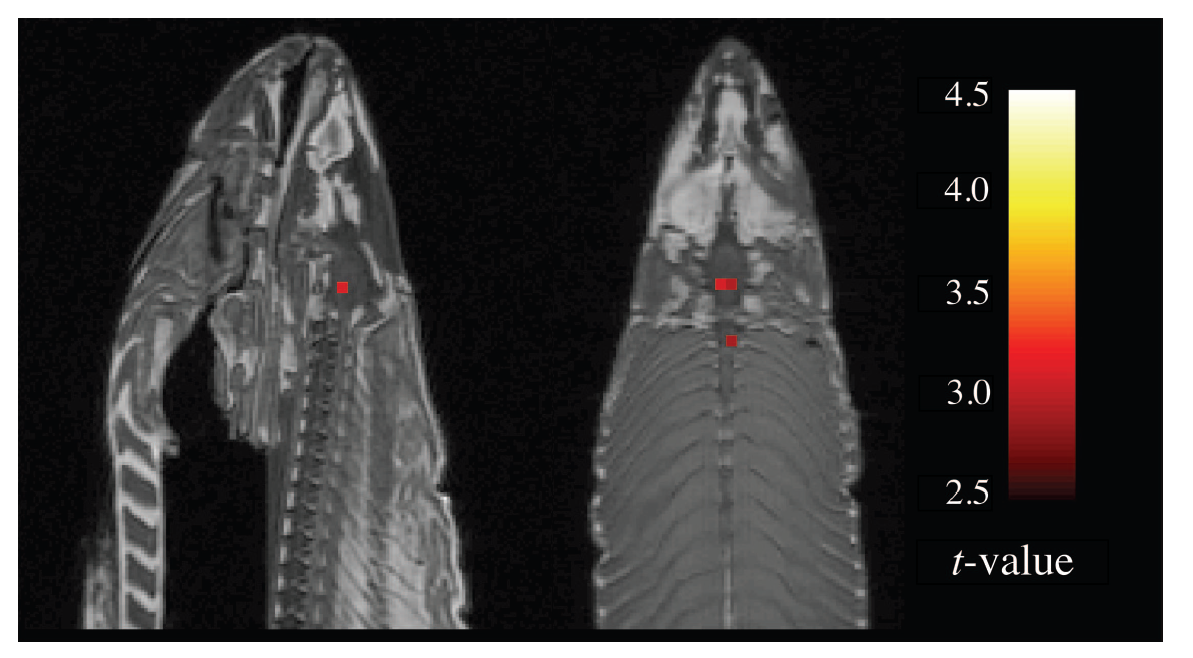
\includegraphics[width=0.75\linewidth]{image//saumon} 

}

\caption{Cognitions sociales d'un saumon atlantique décédés. Tirés de Bennett et al. 2010, p.4}\label{fig:saumon}
\end{figure}

Les points rouges de la Figure \ref{fig:saumon} indiquent les congitions sociales du saumon. Plus sérieusement, ces chercheurs critiquent l'absence de contrôle de l'erreur de type I (faux positif) lors de comparaison multiple. Ce problème est d'autant plus important avec des humains sous IRMf, car ces situations comportent beaucoup de bruit statistiques, contrairement au saumon décédé (qui n'en produit pas du tout). Ils montrent bien qu'en absence de ce contrôle, l'analyse peut fournir des résultats farfelus. Il revient à l'expérimentateur de bien utiliser les analyses statistiques et de savoir ce que le logiciel fait et ne fait pas.

L'étude de \textcite{Bennett10} n'est qu'un canular. Les auteurs ont remporté le prix Ig Nobel en 2012, un prix scientifique pour de vrais chercheurs ayant réalisé une vraie étude \emph{faisant d'abord rire, puis réfléchir}.

En pratique, ce type de problème devrait être marginal\ldots{}

\textcite{Eklund16} tentent de valider les méthodes statistiques derrière l'IRMf à l'aide de données réelles. Ils utilisent des données d'IRMf provenant de 499 personnes saines et en état de repos pour effectuer 3 millions d'analyses de groupes de tâches. En utilisant ces données nulles avec différents plans expérimentaux, ils estiment l'incidence des résultats significatifs (en théorie fixé à 5\% de faux positifs pour un seuil de signification de 5 \%). Toutefois, ils constatent que les progiciels les plus courants pour l'analyse de l'IRMf entraînent des taux de faux positifs allant jusqu'à 70 \%. Ces résultats remettent en question la validité d'un certain nombre d'études utilisant l'IRMf et ont des conséquences importantes sur l'interprétation des résultats de neuro-imagerie.

Cette étude a fait un tollé dans la littérature scientifique. Bien que certains aspects de l'étude soient attaquables, il n'en demeure pas moins qu'elle exacerbe le danger de faire confiance aveuglément aux analyses statistiques.

L'objectif de ce court texte n'est pas de discrédité les analyses statistiques ou les chercheurs qui les emploient. Les statistiques sont très utiles et fournissent de l'information qu'il serait impossible d'obtenir autrement. Il s'agit principalemetn d'une mise en garde justifiant en partie l'approche pédagogique de ce livre.

Il est dit en partie, car le seconde, en filigrane de livre, repose sur la double approche d'apprentissage statistique et programmation. En programmant des modèles statistiques, le lecteur a une plus grande emprise sur ceux-ci. Il peut mieux les utiliser, les étudier et les modifier. Il peut s'en servir pour connaître et apprendre davantage. Certaines boîtes noires resteront irrémédiablement des boîtes noires pour le lecteur, mais plus il les démystifiera, mieux il comprendra ce qui se cache derrière les programmes statistiques.

La première section de ce livre justifie et explique le logiciel \textbf{R} et montre comment l'installer ainsi que quelques rudiments statistiques qui seront fort utiles pour le reste de la lecteur. La seconde section couvre ce qui sera probablement le plus important pour l'utilisateur : l'importation, la gestion et la visualisation des données.

TODO

\hypertarget{part-rudiments}{%
\part{Rudiments}\label{part-rudiments}}

\hypertarget{commencer}{%
\chapter{Commencer}\label{commencer}}

\textbf{R} \autocite{R-base} est un logiciel de programmation statistique libre-accès et un environnement pour la computation statistique et l'affichage graphique. Il s'agit d'un projet GNU qui est similaire au langage et à l'environnement S, développés aux Laboratoires Bell (anciennement AT\&T, aujourd'hui Lucent Technologies) par John Chambers. Créé par \textbf{R}oss Ihaka et \textbf{R}obert Gentleman, \textbf{R} fournit une grande variété de techniques statistiques (modélisation linéaire et non linéaire, analyses statistiques classiques, analyse de séries chronologiques, classification) et graphiques, et est hautement extensible.

\textbf{R} est un logiciel basé sur la syntaxe plutôt qu'une approche pointer-et-cliquer (\emph{point-and-click}) comme les logiciels traditionnels. Il peut être plus effrayant ou apparaître trop complexe pour un nouvel utilisateur, mais une fois apprivoisée, cette bête démontre un bien meilleur potentiel que ce soit en automatisation, en personnalisation, en production de figure de haute qualité, etc. \textbf{R} a l'avantage de mettre en plein contrôle ses utilisateurs. Bref, c'est une créature qu'il vaut la peine de maîtriser.

Les logiciels traditionnelles suspendent trop souvent la réflexion critique. Ils sont dociles. L'usager clique sur les bonnes options et obtient les résultats désirés (espérons-le!). En échange d'une expérience ``simple et intuitive'', ils compromettent l'épanouissement de l'utilisateur et rendent l'analyse statistique comme une boîte noire, un programme dont le fonctionnement ne peut être connu. Sont évacuées toutes connaissances des analyses, seules les entrées et les sorties sont pertinentes.

En se limitant à ces logiciels, les utilisateurs sont également à la merci des compagnies qui les distribuent. Par exemple, elles maintiennent des prix exorbitants pour des licences annuelles, malgré le faible soutien technique, la désuétude ou le manque de mise à jour, la présence de bogues informatiques. Ces problèmes sont monnaie courante bien que la licence ne soit pas de la petite monnaie.

Contrairement aux logiciels traditionnels, \textbf{R} permet de réaliser les analyses, mais aussi de les programmer soi-même, de générer des données propres à un modèle, de rester à jour sur les nouvelles tendances et les découvertes en méthodologie de la recherche, de partager aisément les connaissances et la reproduction d'analyses sophistiquées, et tout cela, gratuitement. Évidemment, cela n'est possible que par l'immense communauté derrière le logiciel.

\hypertarget{pourquoi-r}{%
\section{\texorpdfstring{Pourquoi \textbf{R}?}{Pourquoi R?}}\label{pourquoi-r}}

\textbf{R} est complètement gratuit. Il est le logiciel le plus utilisé parmi les scientifiques de sciences de données, statisticiens, etc. Il est l'exemple ultime d'une plateforme communautaire qui fait mieux que les compétiteurs commerciaux. De plus en plus de personnes migrent vers \textbf{R}, mais peu de ses utilisateurs quittent le logiciel vers un autre. Et plus de personnes se joignent à la communauté, plus il y a de documentation, d'aide, de soutien, que ce soit sous forme de livres, de vidéos, d'article, d'ateliers, de formations. L'expérience \textbf{R} devient de plus en plus accessible aux nouveaux immigrants. Comme le code source est ouvert, ses utilisateurs collaborent à la création de modules augmentant ses capacités qui permettent de résoudre des problèmes de plus en plus sophistiqués (et pas juste en statistiques!). Ces modules sont également gratuits et il y en a littéralement des milliers.

L'avantage de maîtriser \textbf{R}, plus spécifiquement de l'utilisation de syntaxe, pour l'expérimentateur est de rendre l'analyse statistique facilement \emph{transmissible} entre expérimentateur (facilite grandement la collaboration), \emph{reproductible} (vérification et collaboration), \emph{répétable} (pour de nouvelles données ou expériences), et \emph{ajustable} (pour de nouveaux scénarios). Quelqu'un d'autre peut jeter un oeil à l'analyse réalisée et voir exactement ce qui s'est produit, tant dans la gestion du jeu de données que l'analyse et la génération de graphiques. L'analyse peut être reproduite par les pairs, voire répéter si des données supplémentaires ont été recueillies ou si une nouvelle expérience a été réalisée.

Même si \textbf{R} est un langage de programmation et que cela peut en intimider plus d'un, il est relativement intuitif à apprendre et assez simple d'utilisation dans la mesure où les ressources appropriées pour apprendre sont accessibles à l'utilisateur. L'apprentissage de la programmation, même si ce n'est pas en \textbf{R,} permet de mieux comprendre le fonctionnement des ordinateurs en plus de reconsidérer le dogmatisme de tout-puissant ``algorithmes''. Il permettra aussi à l'utilisateur lorsqu'il saura suffisamment maîtriser la bête à créer lui-même la syntaxe qu'il lui permettra de résoudre les problèmes sur lesquels il s'intéresse.

Enfin, \textbf{R} possède un incroyable moteur pour la visualisation de données et de capacités graphiques. Aucun autre logiciel ne lui arrive à la cheville.

\hypertarget{installer-r}{%
\section{\texorpdfstring{Installer \textbf{R}}{Installer R}}\label{installer-r}}

\textbf{R} est compatible pour Windows, Mac et Linux. Pour télécharger le logiciel, il faut se rendre sur le site \url{http://www.r-project.org} et sélectionner les hyperliens ``download R'' ou ``CRAN mirror''. Il faut ensuite choisir un \emph{mirror} de son pays d'origine. Par la suite, la page permet de choisir la version appropriée à son système d'exploitation. Il faut alors suivre les indications.

Il est principalement utilisé en anglais bien qu'on peut le définir en français. La plupart de l'aide sera également en anglais surtout celle pour les analyses avancées. Toutefois, il y a beaucoup de ressources accessibles en ligne en français en ce qui a attrait à l'initiation à \textbf{R}.

\hypertarget{rstudio}{%
\subsection{\texorpdfstring{\textbf{R}Studio}{RStudio}}\label{rstudio}}

Bien que \textbf{R} puisse être utilisé seul, son aspect rudimentaire pourra en inquiéter plus d'un (surtout un.e étudiant.e en sciences humaines et sociales). Le logiciel \textbf{R}Studio permet une utilisation plus fluide et intuitive pour les usagers ayant peu ou pas d'expériences en programmation. \textbf{R}Studio est un environnement de développement intégré (IDE pour \emph{integrated development environment}) pour R. Il comprend une console, un éditeur de mise en évidence de la syntaxe qui prend en charge l'exécution directe du code, ainsi que des outils de traçage, d'historique, de débogage et de gestion de l'espace de travail. Le logiciel est gratuit et libre-accès pour une utilisation personnelle. Il comporte aussi une version commerciale qui nécessite un certain déboursement de fonds.

Pour télécharger le logiciel, il faut se rendre sur le site \url{http:rstudio.com} et naviguez jusqu'au téléchargement du logiciel, ou aller spécifiquement sur \url{https://www.rstudio.com/products/rstudio/download/\#download}, où il sera possible de télécharger la version gratuite de \textbf{R}Studio. \textbf{R}Studio est uniquement disponible en anglais.

\hypertarget{les-avantages-de-rstudio}{%
\subsubsection{\texorpdfstring{Les avantages de \textbf{R}Studio}{Les avantages de RStudio}}\label{les-avantages-de-rstudio}}

L'avantage de \textbf{R}Studio, comparativement à l'utilisation unique de \textbf{R}, est d'offrir une gestion de la console, du script, de l'environnement des variables et des documents externes en une seule interface (et beaucoup d'autres avantages!). En plus de la console (ce que \textbf{R} fournit), \textbf{R}Studio permet l'édition de syntaxe qui pourra être commandée ligne par ligne en utilisant \textbf{CTRL + Enter} (Windows) ou \textbf{CMD + Enter} (MacOS), ce qui pourra s'avérer fort utile lors de la programmation de fonction ou d'analyses de données. \textbf{R}Studio affiche également les variables en mémoire dans le menu \emph{Global Environment}, ce qui permet de suivre l'état de la programmation. Enfin, \textbf{R}Studio affiche dans un quatrième menu les fichiers dans le directoire des fichiers \textbf{R} ce qui permet de voir notamment les jeux de données, mais aussi d'autres fonctions ou scripts. C'est également à cet endroit où l'aide (\emph{help}) sera fournie et les figures (\emph{plot}) affichées.

Tout le contenu du présent ouvrage pourra être réalisé avec \textbf{R} ou avec \textbf{R}Studio, toutefois l'usage de ce dernier sera plus agréable aux lecteurs et lectrices.

Oh! Une autre avantage de \textbf{R}studio est qu'il peut être utiliser comme un éditeur de texte. D'ailleurs, cet ouvrage est complètement rédigé avec \textbf{R}Studio (avec le package \texttt{Rmarkdown}).

\hypertarget{autres-options}{%
\subsection{Autres options}\label{autres-options}}

Il existe plusieurs interfaces utilisateurs graphiques (GUI pour \emph{Graphical User Interface}) pour \textbf{R} comme \emph{R Commander} (certainement l'option la plus connue en sciences humaines et sociales) ou \emph{JASP}, mais aussi plusieurs autres. Ces deux options sont gratuites et libre-accès. Il existe aussi d'autres options payantes. Ces logiciels visent l'utilisation de \textbf{R} par une approche pointer-et-cliquer (\emph{point-and-click}) au travers les analyses plutôt que de recourir à la syntaxe. Ces options plus intuitives pour l'utilisateur sans expérience en programmation auront parfois des effets limitatifs pour des analyses plus avancées et ont comme effet indésirable de promouvoir la boîte noire statistique.

\hypertarget{duxe9marrer-r-ou-rstudio}{%
\section{\texorpdfstring{Démarrer \textbf{R} ou \textbf{R}Studio}{Démarrer R ou RStudio}}\label{duxe9marrer-r-ou-rstudio}}

À l'ouverture de \textbf{R}, le logiciel présente la console, une interface très rudimentaire (et assez déstabilisante pour un logiciel pourtant si promu). Une fois le logiciel ouvert, l'application offre une invitation discrète à écrire des commandes. Le symbole \texttt{\textgreater{}} au bas de la console est une invite (\emph{prompt}) indiquant où taper les commandes. C'est à cette ligne de commande que les expressions seront immédiatement évaluées.

\begin{figure}

{\centering 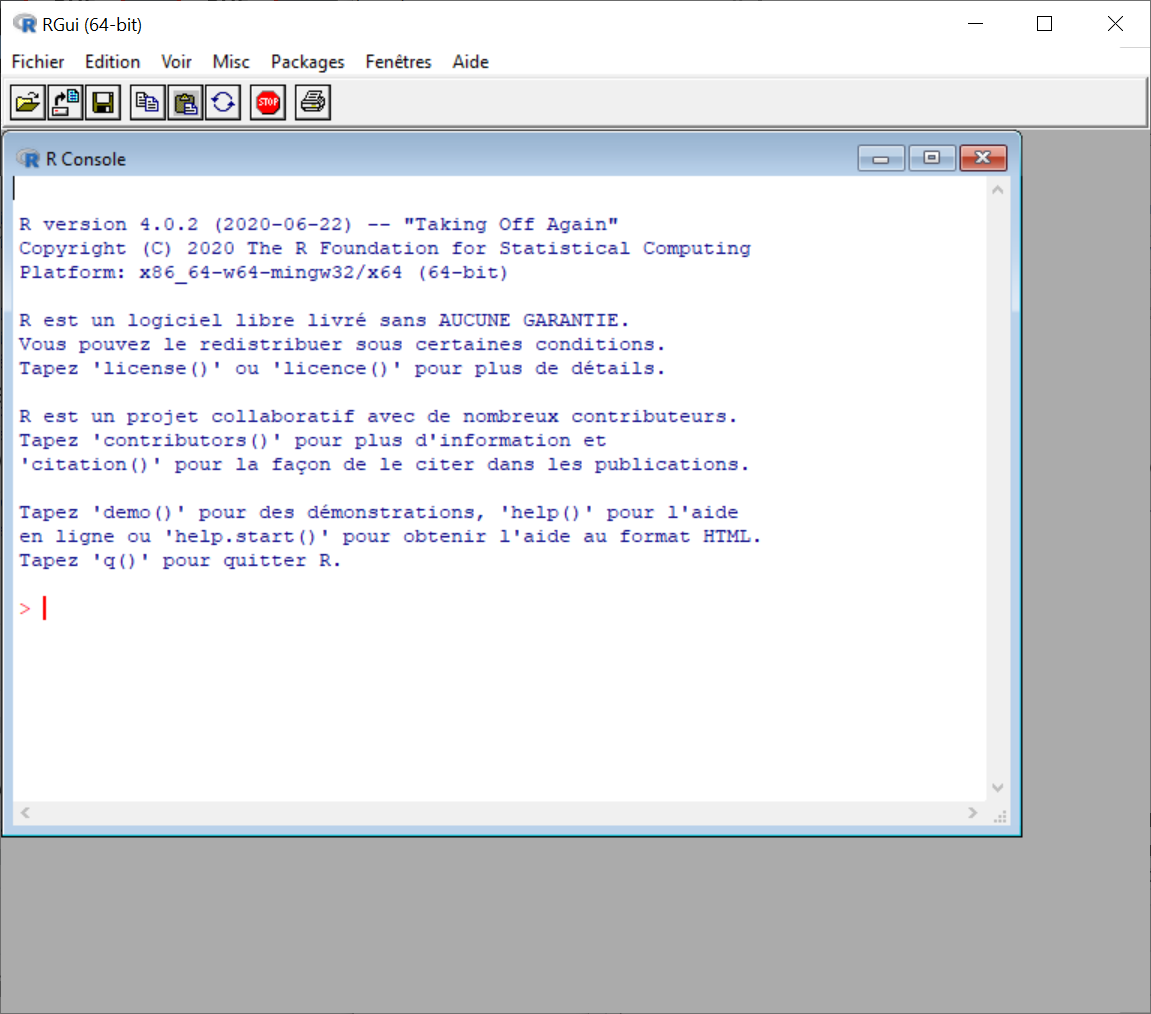
\includegraphics[width=0.75\linewidth]{image//ConsoleR} 

}

\caption{Ouverture (effrayante!) de la console R}\label{fig:ConsoleR}
\end{figure}

Dans la Figure \ref{fig:ConsoleR}, \textbf{R} est défini en français. Cela n'a pour effet que de modifier le menu déroulant (``Fichier, Edition, etc.'') au sommet du logiciel et les différentes options de ce menu. Le fonctionnement reste le même (les fonctions ne sont pas traduites, par exemple).

La console \textbf{R} n'étant pas un éditeur de texte, il faudra enregistrer la syntaxe utilisée lors d'une séance pour la conserver. Le logiciel offre une option d'écriture de script intégré, mais n'est pas lié directement à la console. Il faudra donc se résoudre à abuser du copier-coller ou à sourcer le script (tâche plus ardue pour les nouveaux utilisateurs). Plusieurs éditeurs de texte sont utiles ou même construits pour directement travailler avec \textbf{R}, le plus connu étant certainement \textbf{R}Studio. L'environnement intégré sera beaucoup plus fonctionnel.

La Figure \ref{fig:ConsoleRStudio}, montre l'interface de \textbf{R}Studio, déjà un peu moins intimidante que celle de \textbf{R}. À l'ouverture de \textbf{R}Studio, quatre types de fenêtres sont disponibles : la console (cadran inférieur gauche), les scripts (cadran supérieur gauche), l'environnement (cadran supérieur droit) et l'affichage (cadran inférieur droit). L'emplacement de ces cadrans peut être modifié selon les désirs de l'utilisateur.

\begin{figure}

{\centering 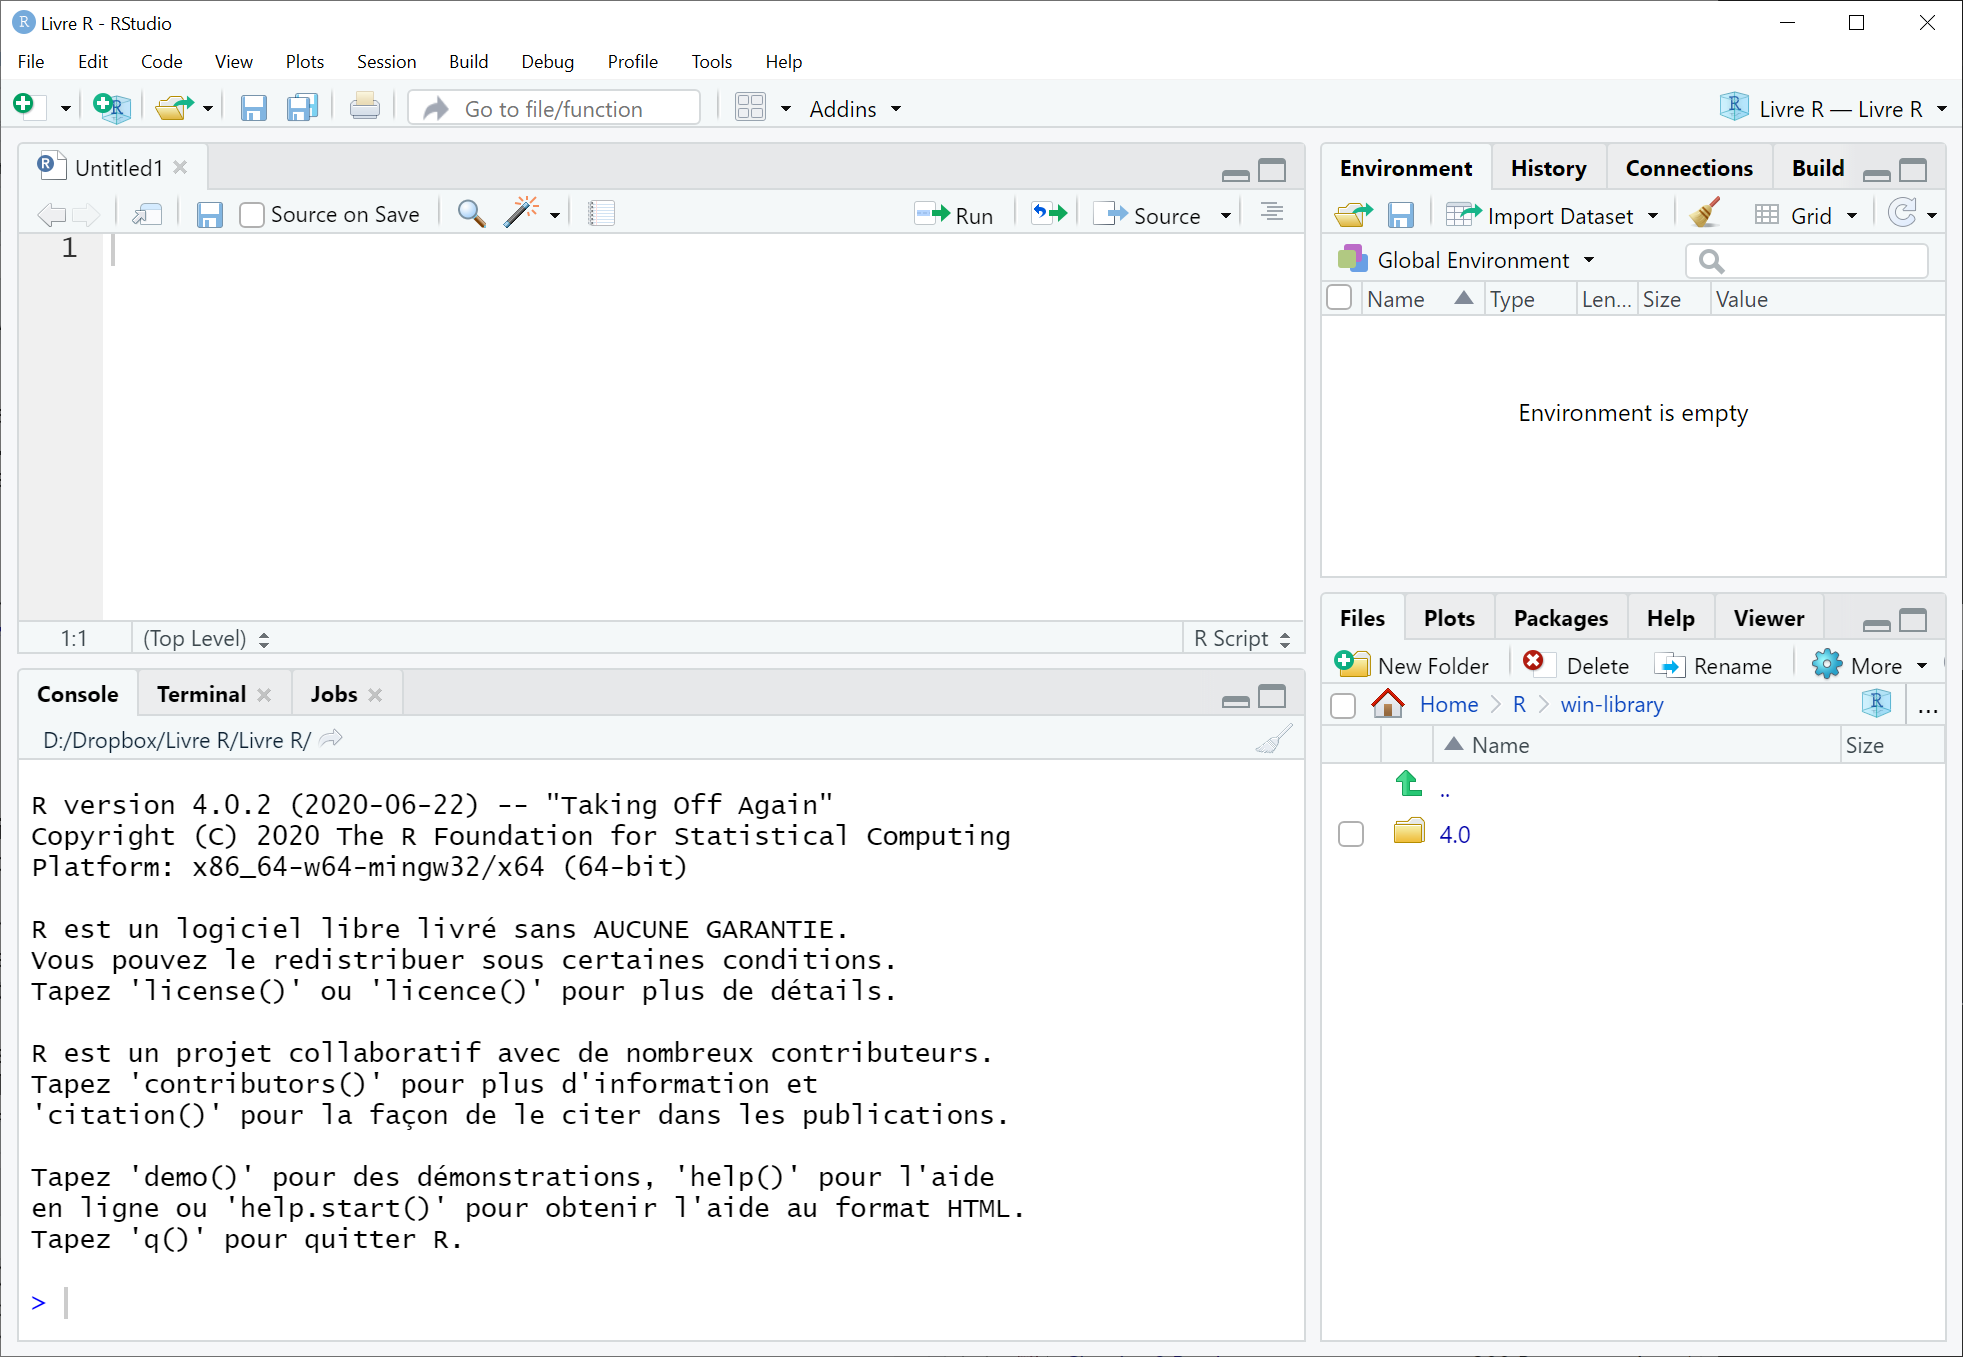
\includegraphics[width=0.75\linewidth]{image//ConsoleRStudio} 

}

\caption{Ouverture (moins effrayante) de **R**Studio}\label{fig:ConsoleRStudio}
\end{figure}

La console \textbf{R}Studio est identique à la console usuelle retrouvée avec \textbf{R}. Elle sert les mêmes fonctions. Le script est un éditeur de texte dans lequel de la syntaxe sera rédigée, sauvegardée, manipulée, et tester. S'il n'est pas ouvert ou s'il faut ouvrir un script supplémentaire, il faut procéder par le menu déroulant.

\begin{quote}
File
New File
R Script
\end{quote}

ou bien \textbf{CTRL + Shift + N}. Il peut y avoir plusieurs scripts ouverts simultanément. L'environnement global permet de connaître les variables et fonctions maison en mémoire vive. L'onglet \emph{History} montre les dernières lignes de code commandées (non affichées dans la figure - il suffit de cliquer sur l'onglet à côté de \emph{Environment}). Enfin, le cadran inférieur droit montre le fichier de travail \textbf{R} qui contiendra ordinairement les fichiers de travail actifs (scripts, jeu de données, fonctions maison, etc.) C'est très utile pour travailler par projet. Si aucun directoire n'est demandé explicitement par \textbf{R} (par exemple, si un jeu de donnée doit être téléchargé), le logiciel cherchera par défaut dans le fichier actif pour télécharger les fichiers demandés. Il est une bonne pratique que de s'assurer d'être dans le bon fichier, car cela pourra causer quelques soucis à l'occasion.

\hypertarget{les-scripts}{%
\section{Les scripts}\label{les-scripts}}

Ce qu'il importe le plus avec \textbf{R}, et ce qui fait resplendir \textbf{R}Studio, est de conserver la syntaxe d'une session à l'autre. Le logiciel ne le fait pas très bien. Il faudra sauvegarder dans un script les expressions et le code utilisés. Ces fichiers ont souvent comme extension ``.R'' et permettront de conserver, voire partager la syntaxe. Il sera possible d'y ajouter des commentaires pour de futures utilisations. Tout éditeur de texte peut permettre la sauvegarde de syntaxe, certains seront mieux que d'autres pour l'utilisation avec \textbf{R}.

\textbf{R}Studio contient déjà un panneau contenant un script qu'il sera possible de sauvegarder et de rouler directement dans la console. Ce dernier est directement lié et il est possible de rouler la syntaxe ligne par ligne avec \textbf{CTRL + Enter} (Windows) ou \textbf{CMD + Enter} (MacOS).

\hypertarget{programmer}{%
\chapter{Programmer}\label{programmer}}

Dans les prochaines sections, les différents éléments de programmation permettant la création et la manipulation de données seront présentés.

\hypertarget{les-variables}{%
\section{Les variables}\label{les-variables}}

Pour manipuler les données, il faut recourir à des variables. Afin de leur attribuer une valeur, il faut assigner cette valeur avec \texttt{\textless{}-} (\textbf{ALT + -}) ou \texttt{=}, par exemple,

\begin{Shaded}
\begin{Highlighting}[]
\NormalTok{a }\OtherTok{\textless{}{-}} \DecValTok{2}
\NormalTok{a}
\CommentTok{\#\textgreater{} [1] 2}
\end{Highlighting}
\end{Shaded}

où \texttt{a} est maintenant égale à \texttt{2}. La première ligne assigne la valeur à \texttt{a}. La deuxième ligne, indique à la console \textbf{R} d'imprimer le résultat pour le voir. Par la suite, \texttt{a} pourra être utilisée dans des fonctions, des calculs ou analyses plus complexes. De surcroît, \texttt{a} pourra devenir une fonction, une chaîne de caractère (\emph{string}) ou un jeu de données.

Conventionnellement, les puristes de \textbf{R} recommanderont l'usage de \texttt{\textless{}-} plutôt que \texttt{=} pour l'assignation. Il y a quelques nuances computationnelles entre les deux, mais qui échapperont irrémédiablement aux néophytes et même aux usagers intermédiaires.

Pour nommer des variables, seuls les caractères alphanumériques peuvent être utilisés ainsi que le tiret bas \texttt{\_} et le \texttt{.}. Les variables ne peuvent commencer par un nombre.

Réassigner une valeur à une variable déjà existante écrase la valeur précédente.

\begin{Shaded}
\begin{Highlighting}[]
\NormalTok{a }\OtherTok{\textless{}{-}} \DecValTok{2}
\NormalTok{a }\OtherTok{\textless{}{-}} \DecValTok{3}
\NormalTok{a}
\CommentTok{\#\textgreater{} [1] 3}
\end{Highlighting}
\end{Shaded}

La sortie produit \texttt{3} et non plus \texttt{2}.

Cette remarque est importante, car elle signifie que l'on peut écraser des fonctions en nommant des variables. Il faut ainsi éviter de nommer des variables avec des fonctions utilisées par \textbf{R}, on évitera notamment l'utilisation des noms suivants.

\begin{Shaded}
\begin{Highlighting}[]
\NormalTok{c; q; t; C; D; I; T; F; pi; mean; var; sd; length; diff; rep;}
\end{Highlighting}
\end{Shaded}

Certains mots seront tout simplement interdits d'utilisation.

\begin{Shaded}
\begin{Highlighting}[]
\ConstantTok{TRUE}\NormalTok{; }\ConstantTok{FALSE}\NormalTok{; }\ControlFlowTok{break}\NormalTok{; }\ControlFlowTok{for}\NormalTok{; }\ControlFlowTok{in}\NormalTok{; }\ControlFlowTok{if}\NormalTok{; }\ControlFlowTok{else}\NormalTok{; }\ControlFlowTok{while}\NormalTok{; }\ControlFlowTok{function}\NormalTok{; }\ConstantTok{Inf}\NormalTok{; }\ConstantTok{NA}\NormalTok{; }\ConstantTok{NaN}\NormalTok{; }\ConstantTok{NULL}\NormalTok{;}
\end{Highlighting}
\end{Shaded}

\hypertarget{les-opuxe9rateurs-arithmuxe9tiques}{%
\section{Les opérateurs arithmétiques}\label{les-opuxe9rateurs-arithmuxe9tiques}}

La première utilisation qu'un nouvel usager fait de \textbf{R} est généralement d'y recourir comme calculatrice. On pourra utiliser les opérateurs arithmétiques de base comme l'addition \texttt{+}, la soustraction \texttt{-}, la multiplication \texttt{*}, la division \texttt{/} , et l'exposant \texttt{\^{}}.

\begin{Shaded}
\begin{Highlighting}[]
\DecValTok{2} \SpecialCharTok{+} \DecValTok{2}
\CommentTok{\#\textgreater{} [1] 4}
\DecValTok{1} \SpecialCharTok{/} \DecValTok{3}
\CommentTok{\#\textgreater{} [1] 0.333}
\DecValTok{2} \SpecialCharTok{*} \DecValTok{3} \SpecialCharTok{+} \DecValTok{2} \SpecialCharTok{\^{}} \DecValTok{2}
\CommentTok{\#\textgreater{} [1] 10}
\end{Highlighting}
\end{Shaded}

Évidemment, ces opérateurs fonctionnent sur des variables numériques.

\begin{Shaded}
\begin{Highlighting}[]
\NormalTok{a }\OtherTok{\textless{}{-}} \DecValTok{1}
\NormalTok{b }\OtherTok{\textless{}{-}} \DecValTok{10}
\NormalTok{a }\SpecialCharTok{/}\NormalTok{ b}
\CommentTok{\#\textgreater{} [1] 0.1}
\end{Highlighting}
\end{Shaded}

Ici, les deux premières lignes assignent des valeurs à \texttt{a} et \texttt{b}, puis imprime la division. L'absence de marqueur \texttt{\textless{}-} ou \texttt{=} indique à \textbf{R} d'imprimer la réponse dans la console. Si le résultat \texttt{a/b} devait être assigné à une variable, alors aucun résultat ne serait affiché, bien que la variable contienne la réponse.

\begin{Shaded}
\begin{Highlighting}[]
\NormalTok{resultat }\OtherTok{\textless{}{-}}\NormalTok{ a }\SpecialCharTok{/}\NormalTok{ b}
\end{Highlighting}
\end{Shaded}

Il n'y a aucune réponse d'affichée. Maintenant, si \texttt{resultat} est demandé, R affiche le résultat.

\begin{Shaded}
\begin{Highlighting}[]
\NormalTok{resultat}
\CommentTok{\#\textgreater{} [1] 0.1}
\end{Highlighting}
\end{Shaded}

D'autres fonctions sont aussi très utiles. Par exemple, la racine carrée \texttt{sqrt()} (qui n'est rien d'autre que \texttt{\^{}(1/2)}) et le logarithme naturel \texttt{log()}. Il suffit d'insérer une variable ou une valeur à l'intérieur d'une de ces fonctions pour en obtenir le résultat.

\begin{Shaded}
\begin{Highlighting}[]
\FunctionTok{sqrt}\NormalTok{(}\DecValTok{4}\NormalTok{)}
\CommentTok{\#\textgreater{} [1] 2}
\DecValTok{4}\SpecialCharTok{\^{}}\NormalTok{(}\DecValTok{1}\SpecialCharTok{/}\DecValTok{2}\NormalTok{)}
\CommentTok{\#\textgreater{} [1] 2}
\FunctionTok{log}\NormalTok{(}\DecValTok{4}\NormalTok{)}
\CommentTok{\#\textgreater{} [1] 1.39}
\end{Highlighting}
\end{Shaded}

\hypertarget{les-commentaires}{%
\section{Les commentaires}\label{les-commentaires}}

Les scripts \textbf{R} peuvent contenir des commentaires. Ceux-ci sont désignés par le désormais célèbre \texttt{\#}. Une ligne de script commençant par ce symbole sera ignorée par la console. Ces commentaires permettent aussi bien de préciser différentes étapes d'un script, que d'expliquer la nomenclature des variables ou encore d'expliquer une fonction, ses entrées, ses sorties. Les commentaires sont extrêmement utiles, car les annotations peuvent souvent sauver énormément de temps et d'effort lors d'utilisations ultérieures.

\begin{Shaded}
\begin{Highlighting}[]
\CommentTok{\# La variable resultat est le quotient des variables a et b}
\NormalTok{resultat }\OtherTok{\textless{}{-}}\NormalTok{ a }\SpecialCharTok{/}\NormalTok{ b}
\NormalTok{resultat}
\CommentTok{\#\textgreater{} [1] 0.1}
\end{Highlighting}
\end{Shaded}

Dans cet exemple, la première ligne est ignorée. Autrement, la console \textbf{R} produirait une erreur, car cette ligne est pour le logiciel pur charabia!

\hypertarget{duxe9finir-une-chauxeene-de-caractuxe8re}{%
\section{Définir une chaîne de caractère}\label{duxe9finir-une-chauxeene-de-caractuxe8re}}

La plupart du temps, les variables utilisées seront numériques, c'est-à-dire qu'elles contiendront des nombres. Parfois en analyses de données, il pourra s'agir de chaîne de caractères (\emph{string}), autrement dit, de mots. Les chaînes de caractères sont définis par le double apostrophe \texttt{"..."}, où on remplace les trois points par les mots désirés.

\begin{Shaded}
\begin{Highlighting}[]
\NormalTok{titre }\OtherTok{\textless{}{-}} \StringTok{"Bonjour le monde!"}
\NormalTok{titre}
\CommentTok{\#\textgreater{} [1] "Bonjour le monde!"}
\end{Highlighting}
\end{Shaded}

\hypertarget{concatuxe9ner}{%
\section{Concaténer}\label{concatuxe9ner}}

Une fonction fort utile permettra de joindre des données dans une seule variable. Précédemment, l'assignation d'une valeur a des variables se limitait qu'à une chaîne de caractères ou une valeur numérique. Pour mettre plusieurs éléments (deux ou plus) dans une seule variable, la fonction concaténée \texttt{c()} (ou combiner, créer) suffira à la tâche. Il faudra délimiter chaque élément par une virgule \texttt{,}.

\begin{Shaded}
\begin{Highlighting}[]
\NormalTok{valeurs }\OtherTok{\textless{}{-}} \FunctionTok{c}\NormalTok{(}\SpecialCharTok{{-}}\DecValTok{5}\NormalTok{, }\DecValTok{5}\NormalTok{)}
\NormalTok{valeurs}
\CommentTok{\#\textgreater{} [1] {-}5  5}
\end{Highlighting}
\end{Shaded}

Elle fonctionne également avec les chaînes de caractères.

\begin{Shaded}
\begin{Highlighting}[]
\NormalTok{texte }\OtherTok{\textless{}{-}} \FunctionTok{c}\NormalTok{(}\StringTok{"Allo"}\NormalTok{, }\StringTok{"le monde"}\NormalTok{)}
\NormalTok{texte}
\CommentTok{\#\textgreater{} [1] "Allo"     "le monde"}
\end{Highlighting}
\end{Shaded}

Et les deux.

\begin{Shaded}
\begin{Highlighting}[]
\NormalTok{phrase }\OtherTok{\textless{}{-}} \FunctionTok{c}\NormalTok{(}\DecValTok{1}\NormalTok{, }\StringTok{"Chat"}\NormalTok{, }\DecValTok{2}\NormalTok{, }\StringTok{"Souris"}\NormalTok{)}
\NormalTok{phrase}
\CommentTok{\#\textgreater{} [1] "1"      "Chat"   "2"      "Souris"}
\end{Highlighting}
\end{Shaded}

Il faudra faire attention à ce qui est passé comme argument à la fonction \texttt{c()}, car elle ne crée que des vecteurs (une ligne en quelque sorte) avec les entrées fournies, peu importe leur structure de départ. Par exemple, un jeu de données passant par \texttt{c()} devient une seule ligne de valeurs. Les fonctions \texttt{cbind()} et \texttt{rbind()} permettront de joindre des colonnes et des lignes respectivement.

\hypertarget{ruxe9fuxe9rer-uxe0-des-sous-uxe9luxe9ments}{%
\section{Référer à des sous-éléments}\label{ruxe9fuxe9rer-uxe0-des-sous-uxe9luxe9ments}}

Avec des variables contenant plusieurs valeurs, il peut être utile de référer à une seule valeur ou un ensemble de valeurs de la variable. Les crochets \texttt{{[}{]}} à la suite du nom d'une variable permettront d'en extraire les valeurs désirées sans tout sortir l'ensemble.

\begin{Shaded}
\begin{Highlighting}[]
\NormalTok{phrase }\OtherTok{\textless{}{-}} \FunctionTok{c}\NormalTok{(}\DecValTok{1}\NormalTok{,}\StringTok{"Chat"}\NormalTok{, }\DecValTok{2}\NormalTok{,}\StringTok{"Souris"}\NormalTok{)}
\CommentTok{\# Extraire le premier élément de la variable phrase}
\NormalTok{phrase[}\DecValTok{1}\NormalTok{]}
\CommentTok{\#\textgreater{} [1] "1"}
\CommentTok{\# Extraire les éléments 1, 2 et 3}
\NormalTok{phrase[}\DecValTok{1}\SpecialCharTok{:}\DecValTok{3}\NormalTok{]}
\CommentTok{\#\textgreater{} [1] "1"    "Chat" "2"}
\CommentTok{\# Extraire les éléments 2 et 4}
\NormalTok{phrase[}\FunctionTok{c}\NormalTok{(}\DecValTok{2}\NormalTok{,}\DecValTok{4}\NormalTok{)]}
\CommentTok{\#\textgreater{} [1] "Chat"   "Souris"}
\CommentTok{\# Ne pas extraire l\textquotesingle{}élément 1}
\NormalTok{phrase[}\SpecialCharTok{{-}}\DecValTok{1}\NormalTok{]}
\CommentTok{\#\textgreater{} [1] "Chat"   "2"      "Souris"}
\CommentTok{\# Ne pas extraire les éléments 1 et 3}
\NormalTok{phrase[}\SpecialCharTok{{-}}\FunctionTok{c}\NormalTok{(}\DecValTok{1}\NormalTok{,}\DecValTok{3}\NormalTok{)]}
\CommentTok{\#\textgreater{} [1] "Chat"   "Souris"}
\end{Highlighting}
\end{Shaded}

Dans le premier exemple, seul un élément est demandé. Dans le deuxième exemple, la commande \texttt{1:3} produit la série de \(1,2,3\) et en extrait ces nombres. Dans le dernier exemple, la fonction \texttt{c()} est astucieusement utilisée pour extraire les éléments \(2\) et \(4\). Le quatrième exemple montre comment retirer un élément en utilisant des valeurs négatives et le cinquième exemple montre comment retirer des éléments.

\hypertarget{les-fonctions}{%
\section{Les fonctions}\label{les-fonctions}}

\textbf{R} offre une multitude de fonctions et permet également à l'usager de bâtir ses propres fonctions (fonctions maison). Elles permettent d'automatiser des calculs (généralement, mais peut faire beaucoup plus!). Tout au long de cet ouvrage, les fonctions seront identifiées par l'ajout de parenthèse à leur fin, comme ceci : \texttt{function()}. Ces fonctions ont généralement la forme suivante.

\begin{Shaded}
\begin{Highlighting}[]
\NormalTok{nom }\OtherTok{\textless{}{-}} \ControlFlowTok{function}\NormalTok{(argument1, argument2, ...) \{}
  \CommentTok{\# Calcul à réaliser}
\NormalTok{\}}
\end{Highlighting}
\end{Shaded}

Ici, \texttt{nom} est le nom auquel la fonction sera référée par la suite, \texttt{function} est la fonction \textbf{R} qui permet de créer la fonction maison, \texttt{argument1} et \texttt{argument2} sont les arguments (les entrées) fournis à la fonction et à partir desquels les calculs seront réalisés, et les accolades \texttt{\{\}} définissent le début et la fin de la fonction dans le script.

Il sera bien utile de créer ses propres fonctions bien que \textbf{R} possède une pléthore de fonctions et de packages en contenant encore plus. Toutes les fonctions, qu'elles soient maisons ou déjà intégrées, respectent le même fonctionnement, ce pour quoi il est utile de s'y pencher. Les fonctions maison permettront d'automatiser certains calculs qui seront propres à résoudre les problèmes de l'usager et d'être réutilisé ultérieurement.

Voici un exemple trivial de fonction. Ici la somme de deux nombres.

\begin{Shaded}
\begin{Highlighting}[]
\NormalTok{addition }\OtherTok{\textless{}{-}} \ControlFlowTok{function}\NormalTok{(a, b) \{}
\NormalTok{  a }\SpecialCharTok{+}\NormalTok{ b}
\NormalTok{\}}
\FunctionTok{addition}\NormalTok{(}\DecValTok{2}\NormalTok{,}\DecValTok{3}\NormalTok{)}
\end{Highlighting}
\end{Shaded}

Par défaut, une fonction retourne la dernière ligne calculée si elle n'est pas assignée à une variable. Si le résultat d'une fonction est assigné, la fonction ne retourne pas le résultat dans la console, mais assigne bel et bien la variable.

\begin{Shaded}
\begin{Highlighting}[]
\NormalTok{addition2 }\OtherTok{\textless{}{-}} \ControlFlowTok{function}\NormalTok{(a, b) \{}
  \CommentTok{\# Le résultat est assigné à une variable}
\NormalTok{  somme }\OtherTok{\textless{}{-}}\NormalTok{ a }\SpecialCharTok{+}\NormalTok{ b}
\NormalTok{\}}

\CommentTok{\# Ne produit pas de sortie}
\FunctionTok{addition2}\NormalTok{(}\DecValTok{100}\NormalTok{, }\DecValTok{241}\NormalTok{)}

\CommentTok{\# Comme il y a assignation, total n\textquotesingle{}est pas affichée}
\NormalTok{total }\OtherTok{\textless{}{-}} \FunctionTok{addition2}\NormalTok{(}\DecValTok{100}\NormalTok{, }\DecValTok{241}\NormalTok{)}

\CommentTok{\# En roulant total, la sortie affiche bien la sortie de addition2()}
\NormalTok{total}
\CommentTok{\#\textgreater{} [1] 341}
\end{Highlighting}
\end{Shaded}

Afin d'éviter ces problèmes ou s'il fallait retourner plusieurs arguments (ce qui sera souvent le cas!), il faudrait utiliser la fonction \texttt{return()} à la fin de la fonction.

\begin{Shaded}
\begin{Highlighting}[]
\NormalTok{addition3 }\OtherTok{\textless{}{-}} \ControlFlowTok{function}\NormalTok{(a, b) \{}
  \CommentTok{\# Le résultat est assigné à une variable}
\NormalTok{  somme }\OtherTok{\textless{}{-}}\NormalTok{ a }\SpecialCharTok{+}\NormalTok{ b}
  \FunctionTok{return}\NormalTok{(somme)}
\NormalTok{\}}

\CommentTok{\# Les deux fonctions produisent une sortie}
\FunctionTok{addition3}\NormalTok{(}\DecValTok{4}\NormalTok{, }\DecValTok{6}\NormalTok{)}
\CommentTok{\#\textgreater{} [1] 10}
\NormalTok{total }\OtherTok{\textless{}{-}} \FunctionTok{addition3}\NormalTok{(}\DecValTok{4}\NormalTok{, }\DecValTok{6}\NormalTok{)}
\NormalTok{total}
\CommentTok{\#\textgreater{} [1] 10}
\end{Highlighting}
\end{Shaded}

\hypertarget{duxe9finir-une-boucle}{%
\section{Définir une boucle}\label{duxe9finir-une-boucle}}

Pour automatiser certains calculer, il peut être utile de recourir à une boucle (\emph{loop}) qui pourra répéter plusieurs fois une même opération. Voici l'anatomie d'une boucle.

\begin{Shaded}
\begin{Highlighting}[]
\ControlFlowTok{for}\NormalTok{(i }\ControlFlowTok{in}\NormalTok{ vec)\{}
  \CommentTok{\# Calcul désiré}
\NormalTok{\}}
\end{Highlighting}
\end{Shaded}

L'élément \texttt{for} est la fonction déclarant la boucle. Les renseignements sur les itérations se retrouvent entre les parenthèses. La variable \texttt{i} prendra successivement tous les éléments dans (\texttt{in}) le vecteur à gauche (\texttt{vec}). Tout le contenu de la boucle (ce qui sera répété) se retrouve entre les accolades \texttt{\{\}}, c'est ce qui sera produit à chaque boucle. Dans cet exemple, la boucle se répète \(k\) fois, soit de \(1,2,3,...,k\), à cause de l'expression \texttt{1:k} qui correspond à générer un vecteur de \(1\) à \(k\). La variable \texttt{i} quant à elle change de valeur à chaque itération. Elle prendra tour à tour ces valeurs chaque itération \(1,2,3,...,k\). La variable pourra judicieusement être utilisée dans la boucle afin de profiter ce comportement, notamment pour le classement des résultats. Lorsque la boucle atteint \(k\), elle se termine.

Il est aussi possible de rédiger la boucle en utilisant uniquement \texttt{k}. Alors, \texttt{i} prendra toutes les valeurs contenues dans \texttt{k}. La longueur du vecteur \texttt{k} définit le nombre d'itérations.

\begin{Shaded}
\begin{Highlighting}[]
\ControlFlowTok{for}\NormalTok{(i }\ControlFlowTok{in}\NormalTok{ k)\{}
  \CommentTok{\# Calcul désiré}
\NormalTok{\}}
\end{Highlighting}
\end{Shaded}

\hypertarget{les-clauses-conditionnelles}{%
\section{Les clauses conditionnelles}\label{les-clauses-conditionnelles}}

Pour réaliser des opérations sous certaines conditions ou opérer des décisions automatiques, il est possible d'utiliser des arguments conditionnels avec des opérateurs logiques. Par exemple, sélectionner des unités ayant certaines caractéristiques, comme les participants ayant 18 ans et moins, les personnes ayant un trouble du spectre de l'autiste, ou encore par sexe. Il est aussi possible d'utiliser les opérateurs pour définir à quelle condition telle ou telle autre fonction doit être utilisée. Il faudra alors utiliser les arguments logiques.

\begin{table}[H]

\caption{\label{tab:unnamed-chunk-22}Symboles logiques et leur signification}
\centering
\begin{tabular}[t]{cc}
\toprule
Symbole & Signification\\
\midrule
== & est égale à\\
!= & n'est pas égale à\\
< & plus petit que\\
> & plus grand que\\
<= & plus petit ou égale\\
\addlinespace
>= & plus grand ou égale\\
\&\& & et\\
|| & ou\\
\bottomrule
\end{tabular}
\end{table}

\textbf{R} teste si les valeurs de la variable correspondent à l'opérateur logique en les déclarant comme vraies (\texttt{TRUE}) ou fausses (\texttt{FALSE}).

\begin{Shaded}
\begin{Highlighting}[]
\NormalTok{valeurs }\OtherTok{\textless{}{-}} \DecValTok{1}\SpecialCharTok{:}\DecValTok{6}
\CommentTok{\# Toutes les valeurs plus grandes que 3.}
\NormalTok{valeurs }\SpecialCharTok{\textgreater{}} \DecValTok{3}
\CommentTok{\#\textgreater{} [1] FALSE FALSE FALSE  TRUE  TRUE  TRUE}
\end{Highlighting}
\end{Shaded}

Cela peut être utilisé pour référer à des sous-éléments comme abordés précédemment.

\begin{Shaded}
\begin{Highlighting}[]
\NormalTok{valeurs }\OtherTok{\textless{}{-}} \DecValTok{1}\SpecialCharTok{:}\DecValTok{6}
\CommentTok{\# Toutes les valeurs plus grandes que 3.}
\NormalTok{valeurs[valeurs }\SpecialCharTok{\textgreater{}} \DecValTok{3}\NormalTok{]}
\CommentTok{\#\textgreater{} [1] 4 5 6}
\end{Highlighting}
\end{Shaded}

Ici, toutes les valeurs vraies de l'opérateur logique sont rapportées.

Les opérateurs logiques servent également à définir des opérations conditionnelles. La fonction \texttt{if} sera alors utilisée. Il y a trois principales formes : \texttt{if} (Si ceci, alors cela), le \texttt{if\ \ else} (Si ceci, alors cela, sinon autre chose) et les échelles \texttt{if\ else\ if\ else}.

\begin{Shaded}
\begin{Highlighting}[]
\ControlFlowTok{if}\NormalTok{(x)\{}
  \CommentTok{\# Opération désirée}
\NormalTok{\}}
\end{Highlighting}
\end{Shaded}

L'anatomie d'une fonction \texttt{if} comporte d'abord la fonction \texttt{if}. L'argument entre parenthèses à sa plus simple expression doit être vérifié par vrai (\texttt{TRUE}) ou faux (\texttt{FALSE}). Si l'argument est vrai, alors le calcul désiré est réalisé, autrement le logiciel ignore le calcul de la fonction entre accolades \texttt{\{\}}.

\begin{Shaded}
\begin{Highlighting}[]
\NormalTok{x }\OtherTok{\textless{}{-}} \SpecialCharTok{{-}}\DecValTok{2}
\ControlFlowTok{if}\NormalTok{(x }\SpecialCharTok{\textless{}} \DecValTok{0}\NormalTok{)\{}
  \FunctionTok{print}\NormalTok{(}\StringTok{"la valeur est négative"}\NormalTok{)}
\NormalTok{\}}
\CommentTok{\#\textgreater{} [1] "la valeur est négative"}
\end{Highlighting}
\end{Shaded}

Il est possible d'élaborer cette logique avec la fonction \texttt{else} qui permet de spécifier une suite à la fonction si l'argument est faux (\texttt{FALSE}).

\begin{Shaded}
\begin{Highlighting}[]
\NormalTok{x }\OtherTok{\textless{}{-}} \DecValTok{2}
\ControlFlowTok{if}\NormalTok{(x }\SpecialCharTok{\textless{}} \DecValTok{0}\NormalTok{)\{}
  \FunctionTok{print}\NormalTok{(}\StringTok{"la valeur est négative"}\NormalTok{)}
\NormalTok{\}}\ControlFlowTok{else}\NormalTok{\{}
  \FunctionTok{print}\NormalTok{(}\StringTok{"la valeur est positive"}\NormalTok{)}
\NormalTok{\}}
\CommentTok{\#\textgreater{} [1] "la valeur est positive"}
\end{Highlighting}
\end{Shaded}

Enfin, il est possible d'élaborer un arbre de décision avec toute une échelle de conditionnels.

\begin{Shaded}
\begin{Highlighting}[]
\NormalTok{x }\OtherTok{\textless{}{-}} \DecValTok{0}
\ControlFlowTok{if}\NormalTok{(x }\SpecialCharTok{\textless{}} \DecValTok{0}\NormalTok{)\{}
  \FunctionTok{print}\NormalTok{(}\StringTok{"la valeur est négative"}\NormalTok{)}
\NormalTok{\}}\ControlFlowTok{else} \ControlFlowTok{if}\NormalTok{(x }\SpecialCharTok{\textgreater{}} \DecValTok{0}\NormalTok{)\{}
  \FunctionTok{print}\NormalTok{(}\StringTok{"la valeur est positive"}\NormalTok{)}
\NormalTok{\}}\ControlFlowTok{else}\NormalTok{\{}
  \FunctionTok{print}\NormalTok{(}\StringTok{"la valeur est égale à 0"}\NormalTok{)}
\NormalTok{\}}
\CommentTok{\#\textgreater{} [1] "la valeur est égale à 0"}
\end{Highlighting}
\end{Shaded}

L'arbre de décision peut devenir aussi compliqué que l'utilisateur le désire : chacune des branches peut contenir autant de ramifications que nécessaire.

Il peut arriver pour certaines fonctions de devoir spécifier si certains paramètres sont vrais (\texttt{TRUE}) ou faux (\texttt{FALSE}) ou de définir des variables ayant ces valeurs. Lorsque c'est le cas, il est toujours recommandé d'écrire les valeurs logiques tout au long comme \texttt{TRUE} et \texttt{FALSE}, même si \textbf{R} reconnaît \texttt{T} et \texttt{F}, car ces dernières peuvent être réassignées, contrairement aux premières.

\hypertarget{les-packages}{%
\section{Les packages}\label{les-packages}}

L'utilisation de packages (souvent nommées bibliothèques, modules, paquets ou paquetage en français - ici, l'usage de \emph{package} sera maintenu) est l'attrait principal de \textbf{R}. Pour éviter l'anglicisme, Antidote suggère \emph{forfait}, \emph{achat groupé} ou \emph{progiciel} (ce dernier étant certainement le terme approprié).

Les packages sont de regroupement de fonctions. C'est certainement l'aspect qui a le plus contribué au succès et à sa dissémination de \textbf{R}. Il s'agit de la mise en commun d'un effort collaboratif afin de créer des fonctions et de les partager librement entre les usagers. Le téléchargement de base de \textbf{R} offre déjà quelques packages rudimentaires (comme \texttt{base} qui offre des fonctions comme \texttt{sum()} ou \texttt{stat} qui offre des fonctions comme \texttt{mean()} et \texttt{var()}), mais qui suffisent rarement lorsque des analyses plus avancées ou plus spécialisées sont nécessaires.

L'une des forces des packages est qu'ils sont fournis généralement avec un bon manuel d'utilisation. Plusieurs contributeurs leur sont associés (avec un responsable). Ils sont maintenus régulièrement. Le soutien des responsables est parfois aisé à obtenir et les auteurs de ces packages sont motivés à maintenir les packages opérationnels et aux bénéfices de tous. La faiblesse des packages est qu'il s'agit malheureusement de \emph{généralement}. Il arrive que certains packages produisent des erreurs de calcul, soient laissé en désuétude par leurs auteurs, que le package ait migré sous une autre forme, que de meilleures options soient disponibles sans aucune notice à cet effet. Cela va sans dire, ce problème concerne les logiciels traditionnels également. Il s'agit toutefois d'un enjeu moindre, car les packages sont souvent recommandés par des collègues, des autorités dans leur domaine respectif ou des ouvrages de référence, ce qui aura comme tendance de promouvoir les meilleurs packages. Pas toujours. Il faut rester critique et ne pas de laisser tromper par une boîte noire.

Une dernière faiblesse : les packages agissent parfois en boîte noire, c'est-à-dire qu'ils court-circuitent la réflexion de l'utilisateur qui leur fait confiance. Il peut être parfois difficile de savoir ce que les fonctions produisent exactement. Au contraire des logiciels traditionnels, ces boîtes noires peuvent dans la plupart des cas être accessibles directement, elles sont liés en plus à des articles scientifiques ou de la documentation qui permet dans comprendre les tenants et aboutissants.

\hypertarget{installer-des-packages}{%
\subsection{Installer des packages}\label{installer-des-packages}}

Pour installer un package, il faut utiliser la fonction

\begin{Shaded}
\begin{Highlighting}[]
\FunctionTok{install.packages}\NormalTok{(}\StringTok{"..."}\NormalTok{)}
\end{Highlighting}
\end{Shaded}

où les \texttt{"..."} doivent être remplacé par le nom du package. Il est important de bien inscrire le nom du package entre guillemet anglophone. Il est aussi possible de sélectionner

\begin{quote}
Tools;
Install Packages\ldots{}
\end{quote}

puis de nommer le package sous l'onglet package. Avec \textbf{R} il faudra auparavant choisir un miroir (sélectionner un pays), ce qui ne sera pas nécessaire avec \textbf{R}Studio. Une fois téléchargé, il ne sera plus nécessaire de refaire cette étape à nouveau, à l'exception de potentielles et ultérieures mises à jour lorsqu'elles devront être réalisées.

\hypertarget{appeler-un-package}{%
\subsection{Appeler un package}\label{appeler-un-package}}

Ce qui n'est pas des plus intuitif avec \textbf{R}, c'est qu'une fois le package téléchargé, il n'est pas directement utilisable. Il faut d'abord l'appeler avec la fonction \texttt{library()}.

\begin{Shaded}
\begin{Highlighting}[]
\FunctionTok{library}\NormalTok{(}\StringTok{"..."}\NormalTok{)}
\end{Highlighting}
\end{Shaded}

Cette étape doit être faite à chaque ouverture de \textbf{R}. Cela permet de ne pas mettre en mémoire trop de package simultanément. Il sera ainsi important d'indiquer tous les packages utilisés en début de script sans quoi des erreurs comme l'absence de fonctions seront produites.

Une technique à laquelle l'utilisateur peut avoir recourt lorsqu'il souhaite n'utiliser qu'une fonction spécifique d'un package est l'utilisation des \texttt{::} débutant par le nom du package suivi par le nom de la fonction, comme \texttt{MASS::mvrnorm()}. La fonction s'utilise de façon usuelle. En utilisant \texttt{::}, il n'est pas nécessaire d'appeler le package avec la fonction \texttt{library()}. Il faut toute fois que le package soit bel et bien installer.

\hypertarget{obtenir-de-laide}{%
\section{Obtenir de l'aide}\label{obtenir-de-laide}}

En utilisant \texttt{help(nom)} ou \texttt{?nom}, où il faut remplacer \texttt{nom} par le nom d'une fonction ou d'un package, \textbf{R} offre de la documentation. Les fonctions d'aide retournent une page de documentation contenant généralement de l'information sur les entrées et les sorties des fonctions. Certaines sont mieux détaillées que d'autres, tout dépendant de leurs créateurs et des personnes qui maintiennent ces fonctions.

\begin{Shaded}
\begin{Highlighting}[]
\CommentTok{\# Obtenir de l\textquotesingle{}aide pour la fonction help()}
\NormalTok{?help}
\end{Highlighting}
\end{Shaded}

Il existe également la fonction \texttt{??nom} qui produit une liste de toutes fonctions \textbf{R} ayant partiellement l'inscription introduite à la place de \texttt{nom}. Aussi, \texttt{example(nom)} produit un exemple d'une fonction.

\hypertarget{en-cas-de-puxe9pins}{%
\section{En cas de pépins}\label{en-cas-de-puxe9pins}}

Il arrive parfois que le code utilisé ne fonctionne pas, que des erreurs se produisent ou que des fonctions fort utiles demeurent inconnues. Même après plusieurs années d'utilisation, les utilisateurs font encore quotidiennement des erreurs (au moins une!). Un excellent outil est d'utiliser un moteur de recherche dans un fureteur de prédilection, de poser une question à l'aide de quelques mots clés bien choisis, préférablement en anglais, et en y inscrivant ``with R'' ou ``in R'' ou ``R''. La plupart du temps, les programmeurs de packages auront une solution sur leur site ou leurs instructions de packages. Il y a aussi des plateformes publiques et en ligne, comme \href{https://stackoverflow.com/}{StackOverflow} qui collectent questions et réponses sur le codage. D'autres utilisateurs peuvent avoir posé la même question et des auteurs de programmes R et d'autres usagers y auront répondu aux bénéfices de tous. Dans le cas d'une solution introuvable, ces mêmes plateformes permettent de poser de nouvelles questions. Il faudra toutefois attendre qu'un usager plus expérimenté prenne le temps d'y répondre.

\hypertarget{calculer}{%
\chapter{Calculer}\label{calculer}}

Dans cette section, les fonctions essentielles couramment utilisées sont présentées en rafale. L'accent est mis sur la définition de la fonction (qu'est-ce qu'elle fait?) et son utilité (à quoi sert-elle?). Pour les fonctions essentielles de nature statistiques (moyennes, médianes, etc.), cette section développe une fonction maison (rédigée par l'utilisateur pour la mettre en pratique) et identifie la fonction déjà implantée en \textbf{R}.

\hypertarget{la-longueur}{%
\section{La longueur}\label{la-longueur}}

La longueur d'une variable correspond au nombre d'éléments qu'elle contient. La fonction \texttt{length()} permettra d'obtenir ce résultat. Ce sera particulièrement utile lorsqu'il faudra calculer, par exemple, le nombre de boucle à réaliser à partir des éléments d'un vecteur ou la taille d'échantillon (le nombre d'unités d'observation d'une variable), bien que \texttt{ncol()} (nombre de colonnes) et \texttt{nrow()} (nombre de lignes) soient plus intuitives pour les matrices et les jeux de données.

La somme d'une chaîne de caractères est toujours de \(1\), peu importe le nombre de caractères. La fonction \texttt{nchar()} produira le nombre de caractères.

Une variable qui existe, mais qui ne contient pas de valeur aura une longueur égale \(0\). Ce type de variable est utile lorsqu'il faut créer une variable qui aura une taille changeant d'une situation à l'autre.

\begin{Shaded}
\begin{Highlighting}[]
\NormalTok{x }\OtherTok{\textless{}{-}} \FunctionTok{c}\NormalTok{(}\DecValTok{1}\NormalTok{, }\DecValTok{2}\NormalTok{, }\DecValTok{3}\NormalTok{)}
\FunctionTok{length}\NormalTok{(x)}
\CommentTok{\#\textgreater{} [1] 3}

\NormalTok{y }\OtherTok{\textless{}{-}} \StringTok{"Bonjour le monde!"}
\FunctionTok{length}\NormalTok{(y)}
\CommentTok{\#\textgreater{} [1] 1}

\FunctionTok{nchar}\NormalTok{(y)}
\CommentTok{\#\textgreater{} [1] 17}
\end{Highlighting}
\end{Shaded}

\hypertarget{la-somme}{%
\section{La somme}\label{la-somme}}

Il est possible de calculer des sommes de variables pour en obtenir le total. En tant qu'humain, le calcul d'une série de nombre correspond à prendre chaque nombre et de les additionner un à un. La fonction suivante reproduit assez bien ce qu'un humain ferait (avec ses quelques caprices de programmation tel que devoir déclarer l'existence de la variable de \texttt{total} et spécifier le nombre d'éléments à calculer).

\begin{Shaded}
\begin{Highlighting}[]
\NormalTok{somme }\OtherTok{\textless{}{-}} \ControlFlowTok{function}\NormalTok{(x)\{}
\NormalTok{  n }\OtherTok{\textless{}{-}} \FunctionTok{length}\NormalTok{(x)}
\NormalTok{  total }\OtherTok{\textless{}{-}} \DecValTok{0}
  \ControlFlowTok{for}\NormalTok{(i }\ControlFlowTok{in} \DecValTok{1}\SpecialCharTok{:}\NormalTok{n)\{}
    \CommentTok{\# Prendre le ie élément et l\textquotesingle{}additionner}
    \CommentTok{\# au total des (i{-}1)e éléments précédents}
\NormalTok{    total }\OtherTok{\textless{}{-}}\NormalTok{ total }\SpecialCharTok{+}\NormalTok{ x[i]}
\NormalTok{  \}}
  \FunctionTok{return}\NormalTok{(total)}
\NormalTok{\}}
\NormalTok{x }\OtherTok{\textless{}{-}} \FunctionTok{c}\NormalTok{(}\DecValTok{1}\NormalTok{,}\DecValTok{2}\NormalTok{,}\DecValTok{3}\NormalTok{,}\DecValTok{4}\NormalTok{,}\DecValTok{5}\NormalTok{,}\SpecialCharTok{{-}}\DecValTok{6}\NormalTok{)}
\FunctionTok{somme}\NormalTok{(x)}
\CommentTok{\#\textgreater{} [1] 9}
\FunctionTok{sum}\NormalTok{(x)}
\CommentTok{\#\textgreater{} [1] 9}
\end{Highlighting}
\end{Shaded}

À noter que l'utilisation de la boucle est à des fins illustratives seulement. En termes de rendement computationnel, elle est bien peu efficace. Il faudra privilégier la fonction \texttt{sum()} pour calculer le total de son entrée.

Il faut prendre garde : \textbf{R} calcule le total de tous les éléments de l'entrée sans égard aux lignes et aux colonnes. Autrement dit, il vectorise les entrées. Si deux variables étaient entrées par inadvertance, alors R calculerait la somme de ces deux variables plutôt que de retourner deux totaux. À cette fin, les fonctions \texttt{rowSums()} et \texttt{colSums()} seront utiles lorsqu'il faudra calculer des sommes sur des lignes (\emph{row}) ou des colonnes (\emph{col}).

\hypertarget{la-moyenne}{%
\section{La moyenne}\label{la-moyenne}}

La moyenne est une mesure de tendance centrale qui représente le centre d'équilibre d'une distribution (un centre de gravité en quelque sorte). Si le poids d'un des côtés d'une distribution de probabilité était altéré (plus lourde ou plus légère), alors la moyenne se déplacerait en conséquence.

La moyenne d'un échantillon correspond à la somme de toutes les unités d'une variable divisée par le nombre de données de cette variable ou, mathématiquement, \[\bar{x}=\frac{\Sigma_{i=1}^n x}{n} \] où \(x\) est la variable, \(n\) est le nombre d'unité et \(\Sigma_i^n\) représente la somme de toutes les unités de \(x\). \textbf{R} possède déjà une fonction permettant de calculer la moyenne sans effort, \texttt{mean()} où l'argument est la variable. Il est possible de développer une fonction maison pour calculer la moyenne comme

\begin{Shaded}
\begin{Highlighting}[]
\NormalTok{x\_bar }\OtherTok{\textless{}{-}} \FunctionTok{sum}\NormalTok{(x)}\SpecialCharTok{/}\FunctionTok{length}\NormalTok{(x)}
\end{Highlighting}
\end{Shaded}

où \texttt{sum(x)} calculer la somme de toutes les unités de \texttt{x}, \texttt{/} permet la division et \texttt{length(x)} calcule le nombre d'unités du vecteur \texttt{x}. Par exemple, à partir d'une variable \texttt{x}, les fonctions suivantes donnent le même résultat. Par contre la fonction \texttt{mean()} est beaucoup plus robuste que cette dernière équation.

\begin{Shaded}
\begin{Highlighting}[]
\CommentTok{\# Création de la variable}
\NormalTok{x }\OtherTok{\textless{}{-}} \FunctionTok{c}\NormalTok{(}\DecValTok{0}\NormalTok{, }\DecValTok{1}\NormalTok{, }\DecValTok{2}\NormalTok{, }\DecValTok{3}\NormalTok{, }\DecValTok{4}\NormalTok{, }\DecValTok{5}\NormalTok{)}

\CommentTok{\# La moyenne}
\FunctionTok{mean}\NormalTok{(x)}
\CommentTok{\#\textgreater{} [1] 2.5}

\CommentTok{\# La moyenne}
\FunctionTok{sum}\NormalTok{(x)}\SpecialCharTok{/}\FunctionTok{length}\NormalTok{(x)}
\CommentTok{\#\textgreater{} [1] 2.5}
\end{Highlighting}
\end{Shaded}

Comme pour \texttt{sum()}, les fonctions \texttt{rowMeans()} et \texttt{colMeans()} seront utiles lorsqu'il faudra calculer des moyennes sur des lignes (\emph{row}) ou des colonnes (\emph{col}).

\hypertarget{la-muxe9diane}{%
\section{La médiane}\label{la-muxe9diane}}

La médiane d'un échantillon correspond à la valeur où \(50\%\) des données se situe au-dessous et au-dessus de cette valeur. C'est la valeur au centre des autres (lorsqu'elles sont ordonnées). Quand le nombre de données est impair, le \(\frac{(n+1)}{2}\)\textsuperscript{e} élément est la médiane. Quand le nombre est pair, la moyenne des deux valeurs au centre correspond à la médiane. Cette statistique est intéressante comme mesure de tendance centrale, car elle est plus robuste aux valeurs aberrantes (moins sensibles) que la moyenne.

Évidemment, \textbf{R} offre déjà une fonction \texttt{median()} pour réaliser le calcul. Il est toutefois possible de programmer une fonction maison. Il faut utiliser la fonction \texttt{sort()} pour ordonner les données (croissant par défaut).

\begin{Shaded}
\begin{Highlighting}[]
\NormalTok{mediane }\OtherTok{\textless{}{-}} \ControlFlowTok{function}\NormalTok{(x) \{}
\NormalTok{  n }\OtherTok{\textless{}{-}} \FunctionTok{length}\NormalTok{(x)}
\NormalTok{  s }\OtherTok{\textless{}{-}} \FunctionTok{sort}\NormalTok{(x)}
  \FunctionTok{ifelse}\NormalTok{(n}\SpecialCharTok{\%\%}\DecValTok{2} \SpecialCharTok{==} \DecValTok{1}\NormalTok{, s[(n }\SpecialCharTok{+} \DecValTok{1}\NormalTok{) }\SpecialCharTok{/} \DecValTok{2}\NormalTok{], }\FunctionTok{mean}\NormalTok{(s[n }\SpecialCharTok{/} \DecValTok{2} \SpecialCharTok{+} \DecValTok{0}\SpecialCharTok{:}\DecValTok{1}\NormalTok{]))}
\NormalTok{\}}

\CommentTok{\# Tester ensuite:}
\NormalTok{x }\OtherTok{\textless{}{-}} \FunctionTok{c}\NormalTok{(}\DecValTok{42}\NormalTok{, }\DecValTok{23}\NormalTok{, }\DecValTok{53}\NormalTok{, }\DecValTok{77}\NormalTok{, }\DecValTok{93}\NormalTok{, }\DecValTok{20}\NormalTok{, }\DecValTok{37}\NormalTok{, }\DecValTok{24}\NormalTok{, }\DecValTok{60}\NormalTok{, }\DecValTok{62}\NormalTok{)}
\FunctionTok{median}\NormalTok{(x)}
\CommentTok{\#\textgreater{} [1] 47.5}
\FunctionTok{mediane}\NormalTok{(x)}
\CommentTok{\#\textgreater{} [1] 47.5}
\end{Highlighting}
\end{Shaded}

L'expression \texttt{n\%\%2}, lue \(n \bmod 2\), joue astucieusement le rôle de vérifier si \texttt{n} est impaire. La formule générale \(x \bmod y\) représente une opération binaire associant à deux entiers naturels le reste de la division du premier par le second. Par exemple, \(60 \bmod 7\), noter \texttt{60\%\%7} dans \textbf{R}, donne \(4\) soit le reste de \(7*8 + 4 = 60\). Le logiciel le confirme.

\begin{Shaded}
\begin{Highlighting}[]
\DecValTok{60}\SpecialCharTok{\%\%}\DecValTok{7}
\CommentTok{\#\textgreater{} [1] 4}
\end{Highlighting}
\end{Shaded}

Il s'agit d'une technique de programmation très pratique. Dans le cas de \texttt{n\%\%2}, la formule donne \(1\) dans le cas d'un nombre impair ou \(0\) dans le cas d'un nombre pair, puis teste ce résultat pour déterminer s'il réalise \texttt{s{[}(n+1)/2{]}} lorsque \texttt{n\%\%2==1}(\texttt{TRUE}) , ce qui correspond à choisir l'élément au centre d'un vecteur de taille impair, ou bien \texttt{mean(s{[}n/2+0:1{]}} lorsque \texttt{n\%\%2==0}(\texttt{FALSE}) , ce qui correspond à choisir les deux éléments au centre d'un vecteur pair et d'en faire la moyenne. Il s'agit de l'une des nombreuses façons selon lesquelles il est possible de programmer la médiane.

\hypertarget{la-variance}{%
\section{La variance}\label{la-variance}}

La variance d'un échantillon est une mesure de dispersion. Elle représente la somme des écarts (distances) par rapport à la moyenne au carré divisée par la taille d'échantillon moins \(1\). Mathématiquement, il s'agit de l'équation \eqref{eq:var}.

\[
s^2 = \frac{1}{n-1}\sum_{i=1}^n(x_i-\bar{x})^2
\label{eq:var}
\]
Il est assez aisé d'élaborer une fonction pour réaliser se calculer avec les fonctions déjà abordées.

\begin{Shaded}
\begin{Highlighting}[]
\NormalTok{variance }\OtherTok{\textless{}{-}} \ControlFlowTok{function}\NormalTok{(x)\{}
\NormalTok{  n }\OtherTok{\textless{}{-}} \FunctionTok{length}\NormalTok{(x)}
\NormalTok{  xbar }\OtherTok{\textless{}{-}} \FunctionTok{mean}\NormalTok{(x)}
\NormalTok{  variance }\OtherTok{\textless{}{-}} \FunctionTok{sum}\NormalTok{((x }\SpecialCharTok{{-}}\NormalTok{ xbar) }\SpecialCharTok{\^{}} \DecValTok{2}\NormalTok{)}\SpecialCharTok{/}\NormalTok{(n }\SpecialCharTok{{-}} \DecValTok{1}\NormalTok{)}
  \FunctionTok{return}\NormalTok{(variance)}
\NormalTok{\}}
\end{Highlighting}
\end{Shaded}

La variance peut aussi être calculée plus efficacement avec la fonction \textbf{R} \texttt{var()}.

\begin{Shaded}
\begin{Highlighting}[]
\NormalTok{x }\OtherTok{\textless{}{-}} \FunctionTok{c}\NormalTok{(}\DecValTok{26}\NormalTok{, }\DecValTok{6}\NormalTok{, }\DecValTok{40}\NormalTok{, }\DecValTok{36}\NormalTok{, }\DecValTok{14}\NormalTok{, }\DecValTok{3}\NormalTok{, }\DecValTok{21}\NormalTok{, }\DecValTok{48}\NormalTok{, }\DecValTok{43}\NormalTok{, }\DecValTok{2}\NormalTok{)}
\FunctionTok{variance}\NormalTok{(x)}
\CommentTok{\#\textgreater{} [1] 300}
\FunctionTok{var}\NormalTok{(x)}
\CommentTok{\#\textgreater{} [1] 300}
\end{Highlighting}
\end{Shaded}

\hypertarget{luxe9cart-type}{%
\section{L'écart type}\label{luxe9cart-type}}

L'écart type d'un échantillon représente la racine carrée de la variance. Elle a une interprétation plus intuitive en tant que mesure de la moyenne des écarts par rapport à la moyenne. Si le calcul avait été entrepris avec les distances par rapport à la moyenne (au lieu des écarts au carré), alors la somme serait toujours de 0, un résultat tout à fait bancal. En prenant la racine carrée des écarts au carré, ce qui constitue une mesure de distance euclidienne, l'écart type devient une mesure de l'étalement de la dispersion autour du centre d'équilibre.

\[
s =\sqrt{s^2}= \sqrt{\frac{1}{n-1}\sum_{i=1}^n(x_i-\bar{x})^2}
\]
Avec \textbf{R}, la fonction de base est \texttt{sd()}. Il est possible de récupérer la fonction maison précédemment rédigée.

\begin{Shaded}
\begin{Highlighting}[]
\NormalTok{ecart.type }\OtherTok{\textless{}{-}} \ControlFlowTok{function}\NormalTok{(x)\{}
\NormalTok{  et }\OtherTok{\textless{}{-}} \FunctionTok{sqrt}\NormalTok{(}\FunctionTok{variance}\NormalTok{(x))}
  \FunctionTok{return}\NormalTok{(et)}
\NormalTok{\}}
\FunctionTok{ecart.type}\NormalTok{(x)}
\CommentTok{\#\textgreater{} [1] 17.3}
\FunctionTok{sd}\NormalTok{(x)}
\CommentTok{\#\textgreater{} [1] 17.3}
\end{Highlighting}
\end{Shaded}

\hypertarget{les-graines}{%
\section{Les graines}\label{les-graines}}

Par souci de reproductibilité, il est possible de déclarer une valeur de départ aux variables pseudoaléatoires, ce que l'on nomme une graine ou \emph{seed} en anglais. Cela permet de toujours d'obtenir les mêmes valeurs à plusieurs reprises, ce qui est très utile lors d'élaboration de simulations complexes ou lorsque des étudiants essaient de répliquer résultat tiré d'un ouvrage pédagogique.

\begin{Shaded}
\begin{Highlighting}[]
\FunctionTok{set.seed}\NormalTok{(}\StringTok{"nombre"}\NormalTok{)}
\end{Highlighting}
\end{Shaded}

Il suffit de spécifier cette commande (en remplaçant \texttt{nombre} par un nombre) en début de syntaxe pour définir la séquence de nombre. Cette fonction sera utilisée à plusieurs reprises dans le but de reproduire les mêmes sorties.

Cette fonction est présentée, car elle reviendra régulièrement dans ce livre pour qu'il soit possible de reproduire et obtenir exactement les mêmes résultats.

\hypertarget{les-distributions}{%
\section{Les distributions}\label{les-distributions}}

Il existe plusieurs distributions statistiques déjà programmées avec \textbf{R}. Voici les principales utilisées dans cet ouvrage.

\begin{table}[H]

\caption{\label{tab:unnamed-chunk-42}Noms des distributions, fonctions et leurs arguments}
\centering
\begin{tabular}[t]{ccc}
\toprule
Distribution & R & Arguments\\
\midrule
binomiale & binom & size, prob\\
Khi-carré & chisq & df, ncp\\
Fisher & f & df1, df2, ncp\\
normale & norm & mean, sd\\
student & t & df, ncp\\
\addlinespace
uniform & unif & min, max\\
\bottomrule
\end{tabular}
\end{table}

Les libellés ci-dessus ne commanderont pas de fonction. Il faut joindre en préfixe à ces distributions l'une des quatre lettres suivantes : \texttt{d}, \texttt{p},\texttt{q}, ou \texttt{r}. La plus simple est certainement \texttt{r} (\emph{random}) qui génère \texttt{n} valeurs aléatoires de la distribution demandée selon les paramètres spécifiés. Les fonctions \texttt{q} (quantile) prennent un argument de 0 à 1 (100\%), soit un percentile et retourne la valeur de la distribution. La fonction \texttt{p} (probabilité) retourne la probabilité cumulative (du minimum jusqu'à la valeur) d'une valeur de cette distribution. Enfin, la lettre \texttt{d} (densité) permet, notamment, d'obtenir les valeurs de densité de la distribution.

Voici un exemple avec la distribution normale.

\begin{Shaded}
\begin{Highlighting}[]
\FunctionTok{set.seed}\NormalTok{(}\DecValTok{9876}\NormalTok{)}

\CommentTok{\# Génère 5 nombres aléatoires en fonction des paramètres}
\FunctionTok{rnorm}\NormalTok{(}\AttributeTok{n =} \DecValTok{5}\NormalTok{, }\AttributeTok{mean =} \DecValTok{10}\NormalTok{, }\AttributeTok{sd =}\NormalTok{ .}\DecValTok{5}\NormalTok{)}
\CommentTok{\#\textgreater{} [1] 10.51  9.42  9.90  9.95 10.01}

\CommentTok{\# Retourne les valeurs associés à ces probabilités}
\FunctionTok{qnorm}\NormalTok{(}\FunctionTok{c}\NormalTok{(.}\DecValTok{025}\NormalTok{,.}\DecValTok{975}\NormalTok{))}
\CommentTok{\#\textgreater{} [1] {-}1.96  1.96}

\CommentTok{\# Retourne la probabilité d\textquotesingle{}obtenir un score de 1.645 et moins}
\FunctionTok{pnorm}\NormalTok{(}\FloatTok{1.645}\NormalTok{)}
\CommentTok{\#\textgreater{} [1] 0.95}

\CommentTok{\# La valeur de la densité de la distribution}
\FunctionTok{dnorm}\NormalTok{(}\DecValTok{0}\NormalTok{)}
\CommentTok{\#\textgreater{} [1] 0.399}
\end{Highlighting}
\end{Shaded}

Ces quatre lettres peuvent être associées à toutes les distributions énumérées et bien d'autres. Elles respectent toutes ce cadre.

\hypertarget{ruxe9puxe9ter-des-valeurs}{%
\section{Répéter des valeurs}\label{ruxe9puxe9ter-des-valeurs}}

La fonction \texttt{rep()} sera utile pour répéter volontairement des valeurs. Il y deux possibilité de répétitions: l'argument \texttt{times} définit le nombre de fois que le vecteur est répété; l'arguement \texttt{each} définit le nombre de fois que chaque élément est répété.

\begin{Shaded}
\begin{Highlighting}[]
\NormalTok{vec }\OtherTok{\textless{}{-}} \FunctionTok{c}\NormalTok{(}\DecValTok{2}\NormalTok{, }\DecValTok{4}\NormalTok{, }\StringTok{"chat"}\NormalTok{)}

\CommentTok{\# Répéter vec trois fois}
\FunctionTok{rep}\NormalTok{(vec, }\AttributeTok{times =} \DecValTok{3}\NormalTok{)}
\CommentTok{\#\textgreater{} [1] "2"    "4"    "chat" "2"    "4"    "chat" "2"    "4"   }
\CommentTok{\#\textgreater{} [9] "chat"}

\CommentTok{\# Répéter chaque éléments de vec trois fois}
\FunctionTok{rep}\NormalTok{(vec, }\AttributeTok{each =} \DecValTok{3}\NormalTok{)}
\CommentTok{\#\textgreater{} [1] "2"    "2"    "2"    "4"    "4"    "4"    "chat" "chat"}
\CommentTok{\#\textgreater{} [9] "chat"}
\end{Highlighting}
\end{Shaded}

\hypertarget{cruxe9ation-dune-matrice}{%
\section{Création d'une matrice}\label{cruxe9ation-dune-matrice}}

La fonction \texttt{matrix()} sera utile pour créer des matrices, commes des matrices de covariances, par exemple. La fonction utilise trois arguments, une matrice de nombre à entrer dans la matrice, un nombre de colonnes et un nombre de lignes. La fonction utilise le recyclage, ce qui pourra être utile à certaines occasions.

\begin{Shaded}
\begin{Highlighting}[]
\CommentTok{\# Une matrice de 0}
\FunctionTok{matrix}\NormalTok{(}\DecValTok{0}\NormalTok{, }\AttributeTok{ncol =} \DecValTok{3}\NormalTok{, }\AttributeTok{nrow =} \DecValTok{3}\NormalTok{)}
\CommentTok{\#\textgreater{}      [,1] [,2] [,3]}
\CommentTok{\#\textgreater{} [1,]    0    0    0}
\CommentTok{\#\textgreater{} [2,]    0    0    0}
\CommentTok{\#\textgreater{} [3,]    0    0    0}

\CommentTok{\# Une matrice contenant les nombres 1:3 pour une matrice 3x3}
\FunctionTok{matrix}\NormalTok{(}\DecValTok{1}\SpecialCharTok{:}\DecValTok{3}\NormalTok{, }\AttributeTok{ncol =} \DecValTok{3}\NormalTok{, }\AttributeTok{nrow =} \DecValTok{3}\NormalTok{)}
\CommentTok{\#\textgreater{}      [,1] [,2] [,3]}
\CommentTok{\#\textgreater{} [1,]    1    1    1}
\CommentTok{\#\textgreater{} [2,]    2    2    2}
\CommentTok{\#\textgreater{} [3,]    3    3    3}

\CommentTok{\# Si la séquence préféré serait de gauche à droite plutôt}
\CommentTok{\# de bas en haut}
\FunctionTok{matrix}\NormalTok{(}\DecValTok{1}\SpecialCharTok{:}\DecValTok{3}\NormalTok{, }\AttributeTok{ncol =} \DecValTok{3}\NormalTok{, }\AttributeTok{nrow =} \DecValTok{3}\NormalTok{, }\AttributeTok{byrow =} \ConstantTok{TRUE}\NormalTok{)}
\CommentTok{\#\textgreater{}      [,1] [,2] [,3]}
\CommentTok{\#\textgreater{} [1,]    1    2    3}
\CommentTok{\#\textgreater{} [2,]    1    2    3}
\CommentTok{\#\textgreater{} [3,]    1    2    3}

\CommentTok{\# Une matrice avec un nombre d\textquotesingle{}entrées égale au nombre de cellule}
\FunctionTok{matrix}\NormalTok{(}\DecValTok{1}\SpecialCharTok{:}\DecValTok{16}\NormalTok{, }\AttributeTok{ncol =} \DecValTok{4}\NormalTok{, }\AttributeTok{nrow =} \DecValTok{4}\NormalTok{)}
\CommentTok{\#\textgreater{}      [,1] [,2] [,3] [,4]}
\CommentTok{\#\textgreater{} [1,]    1    5    9   13}
\CommentTok{\#\textgreater{} [2,]    2    6   10   14}
\CommentTok{\#\textgreater{} [3,]    3    7   11   15}
\CommentTok{\#\textgreater{} [4,]    4    8   12   16}
\end{Highlighting}
\end{Shaded}

Les matrices sont une formes de jeu données dans lequel tous les éléments partagent le même attribut (tous numériques, caractères, logiques, etc.).

\hypertarget{cruxe9ation-dun-jeu-de-donnuxe9es}{%
\section{Création d'un jeu de données}\label{cruxe9ation-dun-jeu-de-donnuxe9es}}

Un jeu de données (\texttt{data.frame}) est un peu comme l'extension de la matrice. La différence étant que les éléments entre les colonnes peuvent partager des attributs différents. Ainsi chaque ligne représente une unité (un participant, un objet) et chaque colonne représente une dimension (informations ou variable) différente de cette objectif. La fonction \texttt{data.frame()} permet de créer de tel objet. La fonction prend comme un argument une série de vecteurs. Si un nom

\begin{Shaded}
\begin{Highlighting}[]
\CommentTok{\# Quelques variables}
\NormalTok{var1 }\OtherTok{\textless{}{-}} \FunctionTok{c}\NormalTok{(}\StringTok{"Éloi"}\NormalTok{, }\StringTok{"Laurence"}\NormalTok{)}
\NormalTok{var2 }\OtherTok{\textless{}{-}} \FunctionTok{c}\NormalTok{(}\DecValTok{6}\NormalTok{, }\DecValTok{3}\NormalTok{)}
\NormalTok{var3 }\OtherTok{\textless{}{-}} \FunctionTok{c}\NormalTok{(}\ConstantTok{TRUE}\NormalTok{, }\ConstantTok{TRUE}\NormalTok{)}

\CommentTok{\# Entrer de trois vecteurs non identifiés}
\NormalTok{jd1 }\OtherTok{\textless{}{-}} \FunctionTok{data.frame}\NormalTok{(var1, var2, var3)}

\CommentTok{\# Entrer de trois vecteurs identifiés}
\NormalTok{jd2 }\OtherTok{\textless{}{-}} \FunctionTok{data.frame}\NormalTok{(}\AttributeTok{nom =}\NormalTok{ var1, }\AttributeTok{age =}\NormalTok{ var2, }\AttributeTok{enfant =}\NormalTok{ var3)}

\CommentTok{\# Comparer}
\NormalTok{jd1 ; jd2}
\CommentTok{\#\textgreater{}       var1 var2 var3}
\CommentTok{\#\textgreater{} 1     Éloi    6 TRUE}
\CommentTok{\#\textgreater{} 2 Laurence    3 TRUE}
\CommentTok{\#\textgreater{}        nom age enfant}
\CommentTok{\#\textgreater{} 1     Éloi   6   TRUE}
\CommentTok{\#\textgreater{} 2 Laurence   3   TRUE}
\end{Highlighting}
\end{Shaded}

En utilisant \texttt{nom.de.variable\ =\ vecteur} à l'intérieur de \texttt{data.frame()}, les noms des colonnes deviennent \texttt{nom.de.variable}. Cela permettra une plus grande flexibilité lorsqu'il faudra \protect\hyperlink{guxe8rer}{gèrer} et \protect\hyperlink{manipuler}{manipuler} les données.

Comme les matrices, les jeux de données ont aussi une restriction. Alors que les jeux de données libérait l'utilisateur de la contrainte d'avoir des objets de même attributs, les jeux de données doivent être créés avec des vecteurs de même longueur. Autrement dit, chaque colonne doit avoir exactement le même nombre de lignes. Parfois, \textbf{R} procédera par recyclage pour combler les éléments. Il faudra donc porter une attention particulière, pour vérifier si c'est l'intention ou non.

\hypertarget{cruxe9ation-dune-liste}{%
\section{Création d'une liste}\label{cruxe9ation-dune-liste}}

Une troisième option pour stocker de informations dans une seule variable est d'avoir recourt au liste. La liste libère à la fois l'utilisateur des objects de mêmes attributs et de même longueur. Pour créer une liste, il faut utiliser la fonction \texttt{list()}. Comme \texttt{data.frame()}, des noms d'éléments peuvent être donner pour chaque liste pour faciliter la manipulation ultérieure de la liste.

\begin{Shaded}
\begin{Highlighting}[]
\CommentTok{\#Quelques variables}
\NormalTok{var1 }\OtherTok{\textless{}{-}} \FunctionTok{c}\NormalTok{(}\StringTok{"chat"}\NormalTok{,}\StringTok{"chien"}\NormalTok{)}
\NormalTok{var2 }\OtherTok{\textless{}{-}} \DecValTok{1}\SpecialCharTok{:}\DecValTok{10}

\CommentTok{\# Entrer de deux vecteurs non identifiés}
\NormalTok{jd1 }\OtherTok{\textless{}{-}} \FunctionTok{list}\NormalTok{(var1, var2)}

\CommentTok{\# Entrer de deux vecteurs identifiés}
\NormalTok{jd2 }\OtherTok{\textless{}{-}} \FunctionTok{list}\NormalTok{(}\AttributeTok{animal =}\NormalTok{ var1, }\AttributeTok{nombre =}\NormalTok{ var2)}

\CommentTok{\# Comparer}
\NormalTok{jd1 ; jd2}
\CommentTok{\#\textgreater{} [[1]]}
\CommentTok{\#\textgreater{} [1] "chat"  "chien"}
\CommentTok{\#\textgreater{} }
\CommentTok{\#\textgreater{} [[2]]}
\CommentTok{\#\textgreater{}  [1]  1  2  3  4  5  6  7  8  9 10}
\CommentTok{\#\textgreater{} $animal}
\CommentTok{\#\textgreater{} [1] "chat"  "chien"}
\CommentTok{\#\textgreater{} }
\CommentTok{\#\textgreater{} $nombre}
\CommentTok{\#\textgreater{}  [1]  1  2  3  4  5  6  7  8  9 10}
\end{Highlighting}
\end{Shaded}

L'utilisation de listes est une caractéristique prédominante avec \textbf{R}. Par exemple, \textbf{R} ne peut sortir qu'une variable par fonction. Si la fonction doit retourner plusieurs éléments, ceux-ci devront se retrouver dans une liste. Ce qui sera plus nébuleux pour le lecteur, c'est que l'optimisation de \textbf{R} se fait par les listes. Cela sera noté aux moments appropriés.

\hypertarget{exercice-rudiments}{%
\chapter*{Exercices}\label{exercice-rudiments}}
\addcontentsline{toc}{chapter}{Exercices}

\begin{enumerate}
\def\labelenumi{\arabic{enumi}.}
\tightlist
\item
  Quel est le résultat de \texttt{mean\ \textless{}-\ c(1,\ 2,\ 3)}? Pourquoi?
\item
  Rédiger une fonction calculant l'hypoténuse d'un triangle rectangle. Rappel, le théorème de Pythagore est \(c^2=a^2+b^2\).
\item
  Rédiger une fonction calculant un score-\(z\) pour une variable. Rappel, un score-\(z\), correspond à \(z=\frac{x-\mu}{\sigma}\).
\item
  Rédiger une fonction calculant la médiane d'une variable (ne recopier pas celle de ce livre).
\item
  Rédiger une fonction pour générer une séquence de Fibonacci (chaque nombre est la somme des deux précédents) jusqu'à une certaine valeur, soit \(1,1,2,3,5,8,...\).
\item
  Rédiger une fonction qui pivote une liste de \(k\) éléments par \(n\). Par exemple, une liste de six (\(k=6\) comme \([1,2,3,4,5,6]\)) pivoté de deux (\(n=2\)) devient (\([3,4,5,6,1,2]\)).
\end{enumerate}

\hypertarget{part-jeux-de-donnuxe9es}{%
\part{Jeux de données}\label{part-jeux-de-donnuxe9es}}

\hypertarget{guxe8rer}{%
\chapter{Gèrer}\label{guxe8rer}}

Réaliser des analyses statistiques et des représentations graphiques nécessitent un jeu de données sur lequel travailler. Après l'ouverture de \textbf{R}, l'usager remarquera aisément que le logiciel n'est pas un tableur (tableau de données), contrairement aux logiciels traditionnels. Cette caractéristique l'a peut-être même frappé à la première ouverture! Pour utiliser données, il faudra les conserver dans un fichier externe de la même façon qu'un script, à l'exception qu'il faudra importer les données pour son utilisation.

Un jeu de données porte généralement les extensions ``.Rdata'', lorsqu'elles proviennent de \textbf{R}, ou d'extensions ``.dat'' et ``.txt''. Évidemment, \textbf{R} permet une grande flexibilité, il est ainsi possible d'exporter et d'importer dans d'autres extensions.

Les extensions ``.Rdata'' sont des environnements \textbf{R}, elles contiennent potentiellement plusieurs variables, comme une séance de travail complète. Elles ont aussi l'avantage que, si l'utilisateur double-clique sur un fichier d'extension ``.Rdata'', celui-ci s'ouvre automatiquement dans l'environnement \textbf{R}.

Il est recommandé de ne jamais manipuler les fichiers de données une fois toutes les vérifications réalisées (absence d'erreur dans les données). Il ne sera jamais nécessaire de modifier ces fichiers avec \textbf{R}. Contrairement aux logiciels traditionnels dans lesquels les modifications sont apportées directement aux valeurs ou ajoutées aux fichiers, cela n'est pas nécessaire dans la mesure où les syntaxes décrivant ces manipulations sont conservées. Il devient impossible d'endommager, de corrompre ou d'altérer le fichier de données. Les données originales restent intactes. Il suffit de les importer puis de commander la syntaxe qui lui est associée pour obtenir de nouveau la version \emph{propre} du jeu de données.

\hypertarget{quelques-conseils-de-gestion}{%
\section{Quelques conseils de gestion}\label{quelques-conseils-de-gestion}}

Voici quelques conseils pour la gestion le jeu de données.

\begin{itemize}
\item
  Éviter les noms trop longs ou trop courts et dépourvus de signification. Cela augmente le risque d'erreur. L'utilisation de huit caractères ou moins est une bonne recommandation (quoique ce n'est pas une règle!). Pour conserver plus de renseignements, utiliser les commentaires de la syntaxe.
\item
  Éviter les espaces entre les mots. Cela peut être interprété erronément comme deux éléments. À la place, collez les mots et distinguer-les avec des majuscules (MaFonction), utiliser le tiret bas (ma\_fonction) ou un point (ma.fonction).
\item
  Éviter les espaces ou les vides dans les données. Cela peut être interprété comme des données (absentes) ou non.
\item
  Éviter les symboles suivants \texttt{?,\ \$,\ \%,\ \^{},\ \&,\ *,\ (,\ ),\ -,\ \#,\ ?,\ ,\ ,\ \textless{},\ \textgreater{},\ /,\ \textbar{},\ \textbackslash{},\ {[},\ {]},\ \{} et \texttt{\}} qui peuvent erronément être interprétés comme de la syntaxe autant dans les noms de variables que dans les données.
\item
  Vérifier que les valeurs manquantes sont identifiées \texttt{NA}.
\item
  Si les données proviennent d'un autre logiciel, vérifier la présence de commentaires qui pourraient occasionner des lignes ou colonnes supplémentaires et ainsi corrompre le jeu de données.
\item
  Vérifier que l'exportation et l'importation se sont bien déroulées.
\end{itemize}

\hypertarget{voir-la-base-de-donnuxe9es}{%
\section{Voir la base de données}\label{voir-la-base-de-donnuxe9es}}

Il est possible de voir les données en utilisant la fonction \texttt{View()} et en y insérant le nom de la variable. Le logiciel afficher un tableur avec les données, dont il sera impossible de modifier les valeurs. Cela peut être utile pour s'assurer que le jeu de données est en ordre, bien importé, ou le consulter.

\hypertarget{sauvegarder-un-jeu-de-donnuxe9es}{%
\section{Sauvegarder un jeu de données}\label{sauvegarder-un-jeu-de-donnuxe9es}}

Si un jeu de données est directement créé avec \textbf{R}, par exemple, les jeux de données artificiels, il est possible de les sauvegarder avec la fonction \texttt{save()} qui enregistre une variable dans un fichier.

\begin{Shaded}
\begin{Highlighting}[]
\FunctionTok{save}\NormalTok{(}\StringTok{"variable"}\NormalTok{, }\AttributeTok{file =} \StringTok{"fichier.Rdata"}\NormalTok{)}
\end{Highlighting}
\end{Shaded}

Il est possible à la fin d'une session de travail de sauvegarder l'environnement dans un fichier \texttt{save.image()}. Ainsi, toutes les variables et fonctions maison sont conservées pour une future utilisation.

\begin{Shaded}
\begin{Highlighting}[]
\FunctionTok{save.image}\NormalTok{(}\AttributeTok{file =} \StringTok{"SessionTravail.Rdata"}\NormalTok{)}
\end{Highlighting}
\end{Shaded}

\hypertarget{jeux-de-donnuxe9es-provenant-de-r-et-de-packages}{%
\section{\texorpdfstring{Jeux de données provenant de \textbf{R} et de packages}{Jeux de données provenant de R et de packages}}\label{jeux-de-donnuxe9es-provenant-de-r-et-de-packages}}

Plusieurs packages offrent en plus des fonctions des jeux de données. Mieux encore! \textbf{R} offre des jeux de données inclus avec le logiciel. La fonction \texttt{data()} permet de voir la liste des jeux de données disponibles. Taper simplement le nom du jeu de données permet de l'utiliser, comme s'il avait été déclaré auparavant.

\begin{Shaded}
\begin{Highlighting}[]
\FunctionTok{head}\NormalTok{(cars)}
\CommentTok{\#\textgreater{}   speed dist}
\CommentTok{\#\textgreater{} 1     4    2}
\CommentTok{\#\textgreater{} 2     4   10}
\CommentTok{\#\textgreater{} 3     7    4}
\CommentTok{\#\textgreater{} 4     7   22}
\CommentTok{\#\textgreater{} 5     8   16}
\CommentTok{\#\textgreater{} 6     9   10}
\end{Highlighting}
\end{Shaded}

La fonction \texttt{head()} introduite ici donne simplement un aperçu des six premières lignes du jeu de données pour ne pas afficher le jeu de données complet (ce qui prendrait beaucoup d'espace inutilement.

Pour consulter tous les jeux de données des packages importés, il est possible d'utiliser cette ligne de code.

\begin{Shaded}
\begin{Highlighting}[]
\FunctionTok{data}\NormalTok{(}\AttributeTok{package =} \FunctionTok{.packages}\NormalTok{((}\AttributeTok{all.available =} \ConstantTok{TRUE}\NormalTok{)))}
\end{Highlighting}
\end{Shaded}

Pour utiliser ces jeux, il faut rendre actif le package associé avec la fonction \texttt{library()}.

\hypertarget{cruxe9ation-des-jeux-de-donnuxe9es-artificielles}{%
\section{Création des jeux de données artificielles}\label{cruxe9ation-des-jeux-de-donnuxe9es-artificielles}}

Une façon rudimentaire et efficace d'obtenir des données avec \textbf{R} est de les créer à l'aide des fonctions génératrices de données pseudoaléatoires.

\begin{Shaded}
\begin{Highlighting}[]
\CommentTok{\# Pour la reproductibilité}
\FunctionTok{set.seed}\NormalTok{(}\DecValTok{142}\NormalTok{)}
\CommentTok{\# Nombre d\textquotesingle{}unité}
\NormalTok{n }\OtherTok{\textless{}{-}} \DecValTok{30}
\CommentTok{\# Identifiant}
\NormalTok{id }\OtherTok{\textless{}{-}} \DecValTok{1}\SpecialCharTok{:}\NormalTok{n}

\CommentTok{\# Variables}
\NormalTok{sexe }\OtherTok{\textless{}{-}} \FunctionTok{rbinom}\NormalTok{(n, }\AttributeTok{size =} \DecValTok{1}\NormalTok{, }\AttributeTok{prob =}\NormalTok{ .}\DecValTok{5}\NormalTok{)}
\NormalTok{QI }\OtherTok{\textless{}{-}}  \FunctionTok{round}\NormalTok{(}\FunctionTok{rnorm}\NormalTok{(}\DecValTok{30}\NormalTok{, }\AttributeTok{mean =} \DecValTok{100}\NormalTok{, }\AttributeTok{sd =} \DecValTok{15}\NormalTok{) }\SpecialCharTok{{-}} \DecValTok{5} \SpecialCharTok{*}\NormalTok{ sexe)}
\CommentTok{\# Être "1" soustrait  5 points au QI en moyenne}
\CommentTok{\# Arrondi avec round()}

\CommentTok{\# Création de le jeu de donnees}
\NormalTok{donnees }\OtherTok{\textless{}{-}}  \FunctionTok{data.frame}\NormalTok{(}\AttributeTok{id =}\NormalTok{ id, }\AttributeTok{sexe =}\NormalTok{ sexe, }\AttributeTok{QI =}\NormalTok{ QI)}
\CommentTok{\# Enregistrement}
\FunctionTok{save}\NormalTok{(donnees, }\AttributeTok{file =} \StringTok{"donnees.Rdata"}\NormalTok{)}
\end{Highlighting}
\end{Shaded}

Et voilà un jeu de données simple et sauvegardé dans le dossier de travail auquel il sera possible de se référer.

Ici, deux nouvelles fonctions sont employées : \texttt{round()} arrondie les valeurs à l'unité et \texttt{data.frame()} crée un le jeu de données. L'utilisation des \texttt{=} permet de directement nommer les variables.

\hypertarget{jeux-de-donnuxe9es-provenant-de-ibm-spss}{%
\subsection{Jeux de données provenant de IBM SPSS}\label{jeux-de-donnuxe9es-provenant-de-ibm-spss}}

Il est possible d'importer des données de IBM SPSS vers \textbf{R}. il faudra quelques manipulations préalables. En ayant le fichier de données IBM SPSS ouvert, il faut cliquer sur ``Enregistrer sous'' sous le menu déroulant ``Fichier''. Par défaut, IBM SPSS choisira toutes les variables, mais il est possible de sélectionner seulement les variables d'intérêt en décochant les variables qu'il n'est pas nécessaire de conserver. Ensuite, sélectionner le type de fichier de sauvegarde doit être ``Tabulé (*.dat)``. IBM SPSS offre également la possibilité d'enregistrer les noms de variables (première option à cocher) et les libellés de valeur. Il suffit maintenant de nommer le fichier et de cliquer sur l'onglet''Enregister''.

En s'assurant que nouveau fichier se trouve dans le répertoire actif de \textbf{R}, il suffit de télécharger le fichier.

\begin{Shaded}
\begin{Highlighting}[]
\FunctionTok{read.table}\NormalTok{(}\AttributeTok{file =} \StringTok{"donnees.tab"}\NormalTok{, }\AttributeTok{header =} \ConstantTok{TRUE}\NormalTok{)}
\end{Highlighting}
\end{Shaded}

L'option \texttt{header} devrait être \texttt{FALSE} si les noms de variables n'ont pas été conservés (première ligne du fichier) .

\hypertarget{jeux-de-donnuxe9es-provenant-de-microsoft-excel}{%
\subsection{Jeux de données provenant de Microsoft Excel}\label{jeux-de-donnuxe9es-provenant-de-microsoft-excel}}

Fichier sous le menu déroulant. Sélectionner comme type de fichier ``Texte Unicode (*.txt)``. Intituler le fichier, puis cliquer sur''Enregister''.

Microsoft Excel sauvegardera l'entièreté de la page active. Il est donc pertinent de créer une feuille Microsoft Excel contenant que les informations à conserver.

Par la suite, en s'assurant que nouveau fichier se trouve dans le répertoire actif de \textbf{R}, il suffit de télécharger le fichier avec \texttt{read.table()} et les arguments convenant au jeu de données.

\hypertarget{importation-de-jeux-de-donnuxe9es-avec-rstudio.}{%
\subsection{\texorpdfstring{Importation de jeux de données avec \textbf{R}Studio.}{Importation de jeux de données avec RStudio.}}\label{importation-de-jeux-de-donnuxe9es-avec-rstudio.}}

\textbf{R}Studio offre une interface simple pour télécharger directement un jeu de de données IBM SPSS, Microsoft Excel, SAS, STATA, et des extensions ``.txt'' et ``.readr''. Il y a même un outil de visualisation pour s'assurer que le tout est en ordre.

\begin{quote}
File
Import dataset
From ``format de fichier''
\end{quote}

où ``format de fichier'' remplace Text, SPSS, Excel et les autres. En indiquant le chemin du fichier, \textbf{R} importera le fichier et fournira une syntaxe afin de conserver l'importation pour de futurs usages.

\hypertarget{manipulation-de-donnuxe9es}{%
\section{Manipulation de données}\label{manipulation-de-donnuxe9es}}

Les tableaux ont généralement deux dimensions (lignes par colonnes). Différents éléments ou groupes d'éléments peuvent être extraits des jeux de données. Plusieurs méthodes peuvent être utiliser en fonction des besoins. Le jeu de données \texttt{cars} sera utilisé à des fins illustratives.

\begin{Shaded}
\begin{Highlighting}[]
\FunctionTok{head}\NormalTok{(cars)}
\CommentTok{\#\textgreater{}   speed dist}
\CommentTok{\#\textgreater{} 1     4    2}
\CommentTok{\#\textgreater{} 2     4   10}
\CommentTok{\#\textgreater{} 3     7    4}
\CommentTok{\#\textgreater{} 4     7   22}
\CommentTok{\#\textgreater{} 5     8   16}
\CommentTok{\#\textgreater{} 6     9   10}
\end{Highlighting}
\end{Shaded}

Elle contient 50 unités d'observation (lignes) et deux variables (colonnes), soit la vitesse (\emph{speed}) et la distance (\emph{dist}).

\hypertarget{ruxe9fuxe9rer-uxe0-une-variable-dans-un-jeu-de-donnuxe9es}{%
\subsection{Référer à une variable dans un jeu de données}\label{ruxe9fuxe9rer-uxe0-une-variable-dans-un-jeu-de-donnuxe9es}}

Il est possible de référer à une variable soit en utilisant l'emplacement de la variable par rapport aux autres en utilisant les crochets ou en utilisant le signe \texttt{\$} puis le nom de la variable après le libellé de le jeu de données. L'opération est fort simple avec le symbole \texttt{\$}.

\begin{Shaded}
\begin{Highlighting}[]
\CommentTok{\# Avec $}
\FunctionTok{head}\NormalTok{(cars}\SpecialCharTok{$}\NormalTok{dist)}
\CommentTok{\#\textgreater{} [1]  2 10  4 22 16 10}
\end{Highlighting}
\end{Shaded}

Précédemment utilisés pour extraire des valeurs dans une variable unidimensionnelle, les \texttt{{[}{]}} peuvent extraire des données sur un tableau en deux dimensions (ligne par colonne). Il faut spécifier la ou les lignes désirées, puis la ou les colonnes désirées entre crochets. Laissez une des dimensions en blanc (vide) indique au logiciel de rapporter toutes les valeurs. Par exemple, pour obtenir le même résultat, \texttt{dist} est la deuxième colonne. Il faut référer entre crochets à la colonne \(2\) et comme toutes les lignes sont désirées, cette dimension reste vide.

\begin{Shaded}
\begin{Highlighting}[]
\CommentTok{\# Entre crochets}
\FunctionTok{head}\NormalTok{(cars[,}\DecValTok{2}\NormalTok{])}
\CommentTok{\#\textgreater{} [1]  2 10  4 22 16 10}
\end{Highlighting}
\end{Shaded}

Il est possible de faire la même chose avec les lignes.

\begin{Shaded}
\begin{Highlighting}[]
\CommentTok{\# Entre crochets}
\NormalTok{cars[}\DecValTok{4}\NormalTok{,]}
\CommentTok{\#\textgreater{}   speed dist}
\CommentTok{\#\textgreater{} 4     7   22}
\end{Highlighting}
\end{Shaded}

Ici, toutes les variables de la 4\textsuperscript{e} unité sont rapportée. Remarquer bien l'absence d'argument après la virgule. La fonction \texttt{head} n'est pas nécessaire ici, car il y a peu d'informations à extraire.

Si certaines valeurs spécifiques étaient désirées, comme la valeur de la 4\textsuperscript{e} unité pour la 2\textsuperscript{e} variable.

\begin{Shaded}
\begin{Highlighting}[]
\CommentTok{\# Entre crochets}
\NormalTok{cars[}\DecValTok{4}\NormalTok{, }\DecValTok{2}\NormalTok{]}
\CommentTok{\#\textgreater{} [1] 22}
\end{Highlighting}
\end{Shaded}

Enfin, à l'intérieur d'un jeu de données, les variables peuvent être commandées avec le signe de \texttt{\$} placé après le nom de la variable suivi du nom de la variable ou encore en identifiant les noms de variables entre crochets.

\begin{Shaded}
\begin{Highlighting}[]
\CommentTok{\# Utilisation du signe $}
\FunctionTok{head}\NormalTok{(cars}\SpecialCharTok{$}\NormalTok{speed)}
\CommentTok{\#\textgreater{} [1] 4 4 7 7 8 9}

\CommentTok{\# Nommer entre crochets}
\FunctionTok{head}\NormalTok{(cars[}\StringTok{"speed"}\NormalTok{])}
\CommentTok{\#\textgreater{}   speed}
\CommentTok{\#\textgreater{} 1     4}
\CommentTok{\#\textgreater{} 2     4}
\CommentTok{\#\textgreater{} 3     7}
\CommentTok{\#\textgreater{} 4     7}
\CommentTok{\#\textgreater{} 5     8}
\CommentTok{\#\textgreater{} 6     9}
\end{Highlighting}
\end{Shaded}

\hypertarget{ruxe9fuxe9rer-uxe0-un-sous-ensemble-dunituxe9.}{%
\subsection{Référer à un sous-ensemble d'unité.}\label{ruxe9fuxe9rer-uxe0-un-sous-ensemble-dunituxe9.}}

Pour référer à des unités ayant certaines caractéristiques, la fonction \texttt{subset()} peut s'avérer utile. Les arguments sont un jeu de données, le deuxième est un opérateur logique en lien avec une variable du jeu de données.

\begin{Shaded}
\begin{Highlighting}[]
\CommentTok{\# Extraire les données pour toutes les unités ayant une vitesse égale à 24}
\FunctionTok{subset}\NormalTok{(cars, speed }\SpecialCharTok{==} \DecValTok{24}\NormalTok{)}
\CommentTok{\#\textgreater{}    speed dist}
\CommentTok{\#\textgreater{} 46    24   70}
\CommentTok{\#\textgreater{} 47    24   92}
\CommentTok{\#\textgreater{} 48    24   93}
\CommentTok{\#\textgreater{} 49    24  120}
\end{Highlighting}
\end{Shaded}

Cette fonction est utile s'il faut extraire les données d'un certain sexe, par exemple.

\hypertarget{nommer-des-variables-dans-un-jeu-de-donnuxe9es}{%
\subsubsection{Nommer des variables dans un jeu de données}\label{nommer-des-variables-dans-un-jeu-de-donnuxe9es}}

Il est possible d'attribuer ou de modifier des noms à des colonnes ou des lignes d'un tableau de données. Les fonctions \texttt{colnames()} et \texttt{rownames()} seront alors utilisées. Contrairement aux autres fonctions, celles-ci se retrouvent à gauche de l'équation.

\begin{Shaded}
\begin{Highlighting}[]
\FunctionTok{colnames}\NormalTok{(cars) }\OtherTok{\textless{}{-}}  \FunctionTok{c}\NormalTok{(}\StringTok{"vitesse"}\NormalTok{, }\StringTok{"distance"}\NormalTok{)}
\FunctionTok{head}\NormalTok{(cars)}
\CommentTok{\#\textgreater{}   vitesse distance}
\CommentTok{\#\textgreater{} 1       4        2}
\CommentTok{\#\textgreater{} 2       4       10}
\CommentTok{\#\textgreater{} 3       7        4}
\CommentTok{\#\textgreater{} 4       7       22}
\CommentTok{\#\textgreater{} 5       8       16}
\CommentTok{\#\textgreater{} 6       9       10}
\end{Highlighting}
\end{Shaded}

Il importe de fournir autant de noms qu'il y a de colonnes (ou lignes), et ce, en chaîne de caractères.

\hypertarget{donnuxe9es-manquantes}{%
\subsection{Données manquantes}\label{donnuxe9es-manquantes}}

Les devis de recherche et les jeux de données empiriques sont rarement parfaits et peuvent souvent contenir des données manquantes. \textbf{R} reconnaît les données manquantes lorsqu'elles sont identifiées comme \texttt{NA} (\emph{not available}). Plusieurs méthodes permettent de gérer les données manquantes. La méthode la plus simple est d'éliminer les unités ayant une donnée manquante, soit la suppression par liste (\emph{listwise suppression}). Les fonctions natives de \textbf{R} recourront à l'argument \texttt{na.rm\ =\ TRUE}. Si cela est impossible, la fonction \texttt{na.omit()} permettra de créer des jeux de données sans les valeurs manquantes.

\begin{Shaded}
\begin{Highlighting}[]
\NormalTok{valeurs }\OtherTok{\textless{}{-}}  \FunctionTok{c}\NormalTok{(}\DecValTok{10}\NormalTok{, }\DecValTok{12}\NormalTok{, }\DecValTok{14}\NormalTok{, }\ConstantTok{NA}\NormalTok{, }\DecValTok{18}\NormalTok{)}
\CommentTok{\# La présence de NA empêche la moyenne d\textquotesingle{}être calculée}
\FunctionTok{mean}\NormalTok{(valeurs)}
\CommentTok{\#\textgreater{} [1] NA}
\CommentTok{\# L\textquotesingle{}argument "na.rm = TRUE" gère les NA}
\FunctionTok{mean}\NormalTok{(valeurs, }\AttributeTok{na.rm =} \ConstantTok{TRUE}\NormalTok{)}
\CommentTok{\#\textgreater{} [1] 13.5}
\CommentTok{\# na.omit omet les valeurs NA dans la nouvelle variable.}
\NormalTok{valeurs.nettoyees }\OtherTok{\textless{}{-}}  \FunctionTok{na.omit}\NormalTok{(valeurs)}
\FunctionTok{mean}\NormalTok{(valeurs.nettoyees)}
\CommentTok{\#\textgreater{} [1] 13.5}
\end{Highlighting}
\end{Shaded}

\hypertarget{entruxe9e-de-donnuxe9es}{%
\section{Entrée de données}\label{entruxe9e-de-donnuxe9es}}

S'il y a bien une caractéristique de \textbf{R} qui rebute les nouveaux utilisateurs, c'est certainement que le logiciel ne soit pas prévu pour la saisie de données ou du moins que cela ne soit pas mis à l'avant-plan. Lorsque le logiciel s'ouvre, que ce soit \textbf{R} ou \textbf{R}Studio, l'aspect \emph{table de données} n'existe pas. L'utilisateur pour qui il s'agit de sa première utilisation (et habitué à des logiciels traditionnels) reste pantois : où les données sont-elles entrées?

\hypertarget{entruxe9e-de-donnuxe9es-avec-data.entry-r-de-base}{%
\subsection{\texorpdfstring{Entrée de données avec \texttt{data.entry()} (R de base)}{Entrée de données avec data.entry() (R de base)}}\label{entruxe9e-de-donnuxe9es-avec-data.entry-r-de-base}}

De base, \textbf{R} offre la possibilité d'entrer des données dans un tableur avec la commande \texttt{jd\ =\ data.entry()}. Si une base de données est demandée comme argument (p.~ex., \texttt{data.entry(data\ =\ jd)}), alors le jeu de données est ouvert. Il est aussi possible d'ouvrir le fichier avec des variables déjà créées avec \textbf{R}. Si un tableur vierge est désiré, alors taper \texttt{data.entry(1)} dans la console ouvrira le tableur avec une seule valeur (\texttt{1}), L'utilisateur peut alors modifier les noms de colonnes et entrer les données comme il le ferait avec un logiciel traditionnel. Comme il est possible de le voir à la Figure \ref{fig:dataentry}, l'interface est bien moins attrayante que ses compétiteurs.

\begin{figure}

{\centering 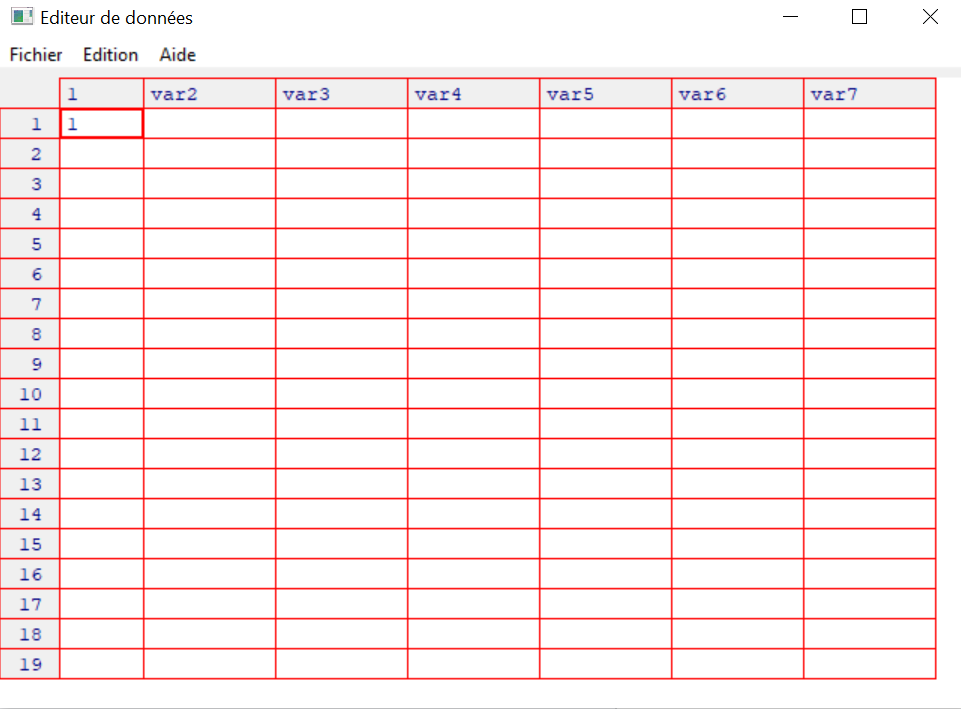
\includegraphics[width=0.75\linewidth]{image//data_entry} 

}

\caption{Ouverture du tableur R}\label{fig:dataentry}
\end{figure}

Lorsque l'entrée de données est terminée, l'utilisateur doit sauvegarder le jeu de données ou l'environnement de travail qui pourront être importés pour de futures utilisations ou entrées. En général, l'utilisateur qui entre manuellement ces données préférera certainement un autre tableur, mais \textbf{R} est certainement en mesure de faire ce travail.

\hypertarget{entruxe9e-de-donnuxe9es-avec-data_edit-package-dataeditr}{%
\subsection{\texorpdfstring{Entrée de données avec \texttt{data\_edit} (package \texttt{DataEditR})}{Entrée de données avec data\_edit (package DataEditR)}}\label{entruxe9e-de-donnuxe9es-avec-data_edit-package-dataeditr}}

Depuis tout récemment (juillet 2021), il existe un package qui permet de faire l'entrée de données en tableur avec \textbf{R}. Il s'agit du package \texttt{DataEditR} \autocite{DataEditR}, une interface utilisateur graphique. Il résout l'un de plus grands défis lorsqu'un utilisateur migre des tableurs traditionnels vers \textbf{R}, c'est-à-dire d'accomplir la transition d'une feuille de calcul interactive où il est possible de pointer et cliquer pour modifier, ajouter, supprimer des donnes vers un mode strict de syntaxe.

Pour démarrer, il faut d'abord installer le package, puis l'appeler. Pour commencer à entrer des données, la syntaxe \texttt{data\_edit()} est suffisante. Pour ouvrir un jeu de données, il suffit de l'ajouter en argument \texttt{data\_edit(jd)}.

Une fois l'interface ouvert, il est possible de manipuler le jeu de données avec les options affichés et avec le clic droit qui permettra notamment d'ajouter des lignes et des colonnes.

\begin{Shaded}
\begin{Highlighting}[]
\CommentTok{\# Pour installer le package}
\FunctionTok{install.packages}\NormalTok{(}\StringTok{"DataEditR"}\NormalTok{)}

\CommentTok{\# Pour rendre la package accessible}
\FunctionTok{library}\NormalTok{(}\StringTok{"DataEditR"}\NormalTok{)}

\CommentTok{\# La fonction}
\FunctionTok{data\_edit}\NormalTok{()}
\end{Highlighting}
\end{Shaded}

Il est recommandé de ne laisser que les données brutes, toutes les modifications et manipulations devraient rester en syntaxe \textbf{R} dans un script associé au jeu de données. Lorsque les entrées sont terminées, il faut simplement sauvegarder la base de données, préférablement en extension .csv. Il est aussi possible de sortir le tableur en tableau de données en assignant la fonction à une variable comme \texttt{jd\ =\ data\_edit()}.

\begin{figure}

{\centering 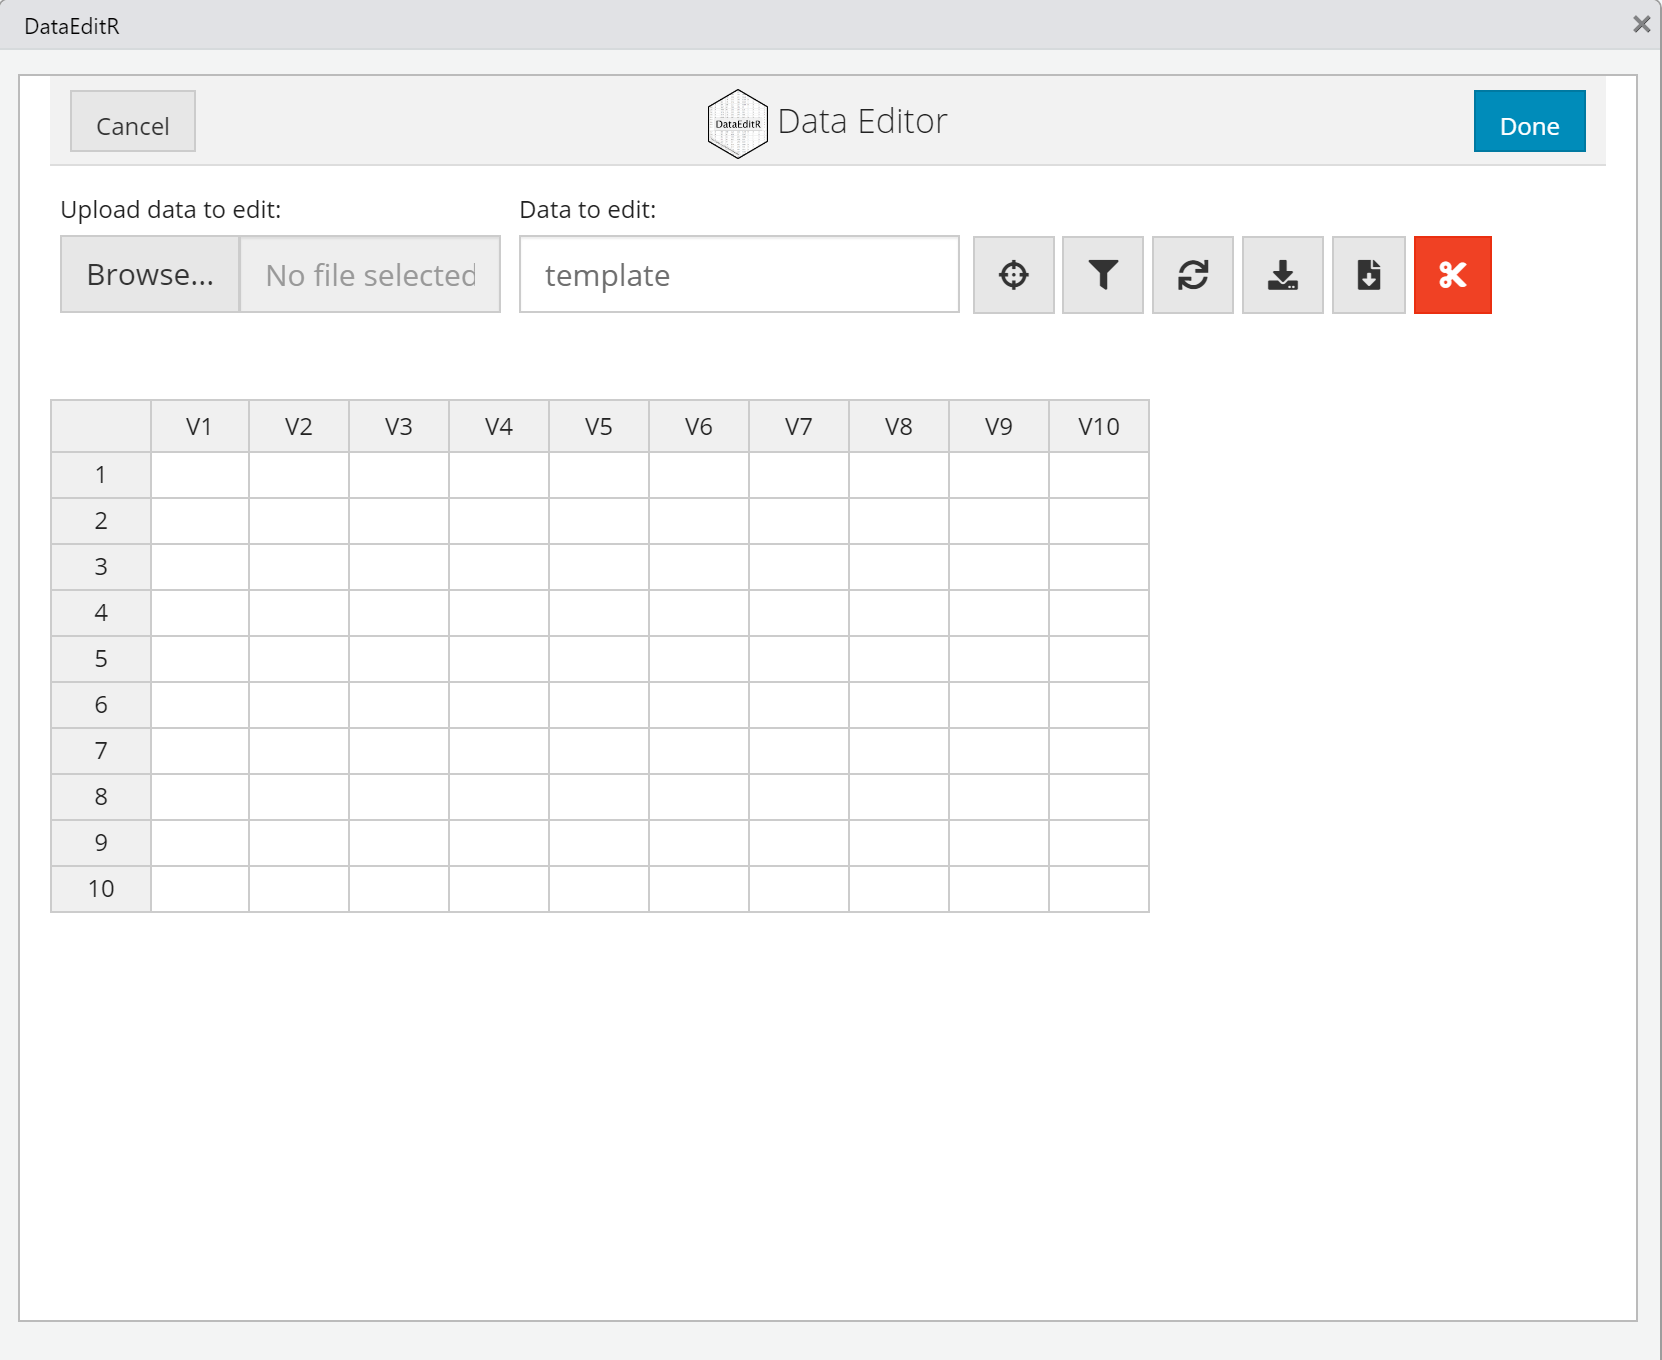
\includegraphics[width=0.75\linewidth]{image//editR} 

}

\caption{Ouverture du tableur de DataEditR}\label{fig:editr}
\end{figure}

En général, l'utilisateur importera ces données dans l'environnement \textbf{R}. Il devra même le faire avec \texttt{data\_edit()} à chaque ouverture d'un nouvelle séance, pour poursuivre l'entrée ou réaliser des manipulations.

\hypertarget{importer}{%
\chapter{Importer}\label{importer}}

Dans la plupart des situations, les analyses et les graphiques seront réalisés à partir d'un jeu de données se trouvant dans un fichier. Ce devra être importé en \textbf{R} pour être manipulé. Les jeux de données peuvent se trouver dans un fichier dans l'ordinateur, mais aussi sur le web. Ils peuvent être en différents types de format.

Dans le premier chapitre, une méthode est présentée pour importer des données. Lorsqu'il provenait d'un logiciel comme IBM SPSS ou Excel, l'accent était mis sur l'exportation de ces données dans un certain format, puis l'importation avec \textbf{R}. Il n'est pas toujours nécessaire d'exporter ces données, puisque le logiciel à l'aide des fonctions de base ou de packages peut lire des fichiers d'une multitude d'extensions.

Pour la description de l'importation, l'ouvrage tient pour acquis que le fichier de données se retrouve dans le directoire de travail (ce qui est l'idéal en général). Un peu plus loin, la création de trajectoires pour différents emplacements sera présentée.

Les fonctions de base permettront d'importer la plupart des jeux de données, particulièrement s'ils ont été exportés dans un format compatible. Pour le cas où ces fichiers ne pourraient être exportés de cette façon, des packages pallieront ce besoin. Dans cet ouvrage, seule une présentation sommaire de ces options sera discutée, l'utilisateur est recommandé à la documentation de ces packages pour plus d'informations.

La prochaine section décrit les fonctions pour importer les bases de données ``manuellement''. En plus de ces méthodes, \textbf{R}Studio possède une interface permettant l'importation des données.

\hypertarget{la-fonction-de-base}{%
\section{La fonction de base}\label{la-fonction-de-base}}

La fonction de base \texttt{read.table()} permettra d'importer la plupart des jeux de données. C'est d'ailleurs ce qui a été présenté sommairement dans le chapitre sur les rudiments. Parfois, ceux-ci ont certaines caractéristiques qu'il faudra préciser comme argument à la fonction \texttt{read.table()} pour assurer une importation adéquate. Ces caractéristiques sont \texttt{header\ =\ FALSE}, \texttt{sep\ =\ ""}, et \texttt{fill\ =\ !blank.lines.skip} (les éléments à droite sont les options par défaut).

Parfois, certains fichiers sauvegardent le nom des variables en tête de colonne (première ligne). Par défaut, \textbf{R} assume qu'il s'agit de valeurs. L'argument \texttt{header\ =\ TRUE} ajouté à \texttt{read.table()} précisera à \textbf{R} lors de l'important que ces libellés sont des noms de colonnes.

Si un autre symbole est utilisé pour délimiter (séparer) des valeurs dans le fichier, comme \texttt{;}ou \texttt{,}, l'argument \texttt{sep\ =\ ";"} ou \texttt{sep\ =\ ","} précisera le séparateur.

Si les lignes du fichier sont de tailles inégales, \textbf{R} assumera qu'il s'agit de valeur, et ces \emph{blancs} de texte seront ajoutés comme valeurs (\texttt{""}). Pour gérer cette situation, l'argument \texttt{fill\ =\ FALSE} devrait régler la situation.

\hypertarget{fichiers-dextension-.txt}{%
\section{Fichiers d'extension .txt}\label{fichiers-dextension-.txt}}

Un fichier d'extension \texttt{.txt} est un fichier texte délimité par des tabulations (\emph{tab-delimited text files}) et est importé à l'aide de la fonction \texttt{read.table()}.

\begin{Shaded}
\begin{Highlighting}[]
\NormalTok{jd }\OtherTok{=} \FunctionTok{read.table}\NormalTok{(}\StringTok{"fichier.txt"}\NormalTok{)}
\end{Highlighting}
\end{Shaded}

\hypertarget{fichiers-dextension-.dat}{%
\section{Fichiers d'extension .dat}\label{fichiers-dextension-.dat}}

Un fichier d'extension \texttt{.dat} est un fichier générique de données et est importé à l'aide de la fonction \texttt{read.table()}.

\begin{Shaded}
\begin{Highlighting}[]
\NormalTok{jd }\OtherTok{=} \FunctionTok{read.table}\NormalTok{(}\StringTok{"fichier.dat"}\NormalTok{)}
\end{Highlighting}
\end{Shaded}

\hypertarget{fichiers-dextension-.csv}{%
\section{Fichiers d'extension .csv}\label{fichiers-dextension-.csv}}

Un fichier d'extension .csv use généralement de séparateur comme \texttt{";"} (lorsque le système numérique de la langue d'origine utilise la virgule - comme le français par exemple) ou \texttt{","} (pour les autres langues qui n'utilise pas la virgule) et ont généralement les noms de variables en première ligne. Ainsi, la fonction \texttt{read.table()} est utilisable pourvu que le séparateur soit précisé et la présence d'en-tête également.

\begin{Shaded}
\begin{Highlighting}[]
\NormalTok{jd }\OtherTok{=} \FunctionTok{read.table}\NormalTok{(}\StringTok{"fichier.csv"}\NormalTok{, }\AttributeTok{sep =} \StringTok{";"}\NormalTok{, }\AttributeTok{header =} \ConstantTok{TRUE}\NormalTok{)}
\end{Highlighting}
\end{Shaded}

Il existe aussi la fonction \texttt{read.csv()} et \texttt{read.csv2()} pour importer des fichiers d'extension \texttt{.csv}. Il s'agit exactement de \texttt{read.table()} à l'exception des arguments par défaut, mais précisant par défaut \texttt{header\ =\ TRUE} et \texttt{fill\ =\ TRUE} et détecte s'il s'agit de \texttt{";"} ou \texttt{","}.

\hypertarget{fichiers-duxe9limituxe9s}{%
\section{Fichiers délimités}\label{fichiers-duxe9limituxe9s}}

Pour les fichiers recourant à un autre caractère qu'une tabulation, qu'une \texttt{","}, ou un \texttt{";"} pour délimiter les valeurs, spécifier le caractère dans \texttt{read.table()} importera le fichier.

\begin{Shaded}
\begin{Highlighting}[]
\NormalTok{jd }\OtherTok{=} \FunctionTok{read.table}\NormalTok{(}\StringTok{"fichier.txt"}\NormalTok{, }\AttributeTok{sep =} \StringTok{"$"}\NormalTok{)}
\end{Highlighting}
\end{Shaded}

Comme pour \texttt{read.csv()} et \texttt{read.csv2()}, les fonctions \texttt{read.delim()} et \texttt{read.delim()} pourraient être utilisées.

\hypertarget{fichiers-dextension-.sav-.dta-.syd-et-.mtp}{%
\section{Fichiers d'extension .sav, .dta, .syd et .mtp}\label{fichiers-dextension-.sav-.dta-.syd-et-.mtp}}

Comme le lecteur s'en doute peut-être, \textbf{R} de base ne permet pas d'importer des fichiers spécifiques d'autres logiciels. Par contre, avec les années se sont développés des packages permettant de pallier la situation. Le package \texttt{foreign} permet d'importer des fichiers issus de IBM SPSS (\texttt{.sav}), Stata (\texttt{.dta}) et Systat (\texttt{.syd}) et Minitab (\texttt{mtp}) avec, respectivement les fonctions \texttt{read.spss()}, \texttt{read.data()}, \texttt{read.systat()} et \texttt{read.mtp()}. La logique d'importation est la même pour ces quatre fonctions.

Pour \texttt{read.spss()}, deux arguments sont importants à souligner. Par défaut, la fonctionne ne retourne pas un \emph{data frame} et utilise les libellés de valeurs (\emph{value labels}). Dans la plupart des cas, l'utilisateur désire probablement obtenir un jeu de données de type \emph{data.frame} et les valeurs sous-jacentes au libellés de valeurs. L'utilisateur peut alors changer ces arguments \texttt{to.data.frame\ =\ TRUE} (par défaut \texttt{FALSE}) et \texttt{use.value.labels\ =\ FALSE}(par défaut \texttt{TRUE}).

\begin{Shaded}
\begin{Highlighting}[]
\FunctionTok{library}\NormalTok{(foreign)}

\CommentTok{\# SPSS}
\NormalTok{jd }\OtherTok{=} \FunctionTok{read.spss}\NormalTok{(}\StringTok{"fichier.sav"}\NormalTok{,}\AttributeTok{to.data.frame =} \ConstantTok{TRUE}\NormalTok{,}\AttributeTok{use.value.labels =} \ConstantTok{FALSE}\NormalTok{)}

\CommentTok{\# Stata}
\NormalTok{jd }\OtherTok{=} \FunctionTok{read.dta}\NormalTok{(}\StringTok{"fichier.dta"}\NormalTok{)}

\CommentTok{\# Systat}
\NormalTok{jd }\OtherTok{=} \FunctionTok{read.systat}\NormalTok{(}\StringTok{"fichier.syd"}\NormalTok{) }

\CommentTok{\# Minitab}
\NormalTok{jd }\OtherTok{=} \FunctionTok{read.mtp}\NormalTok{(}\StringTok{"fichier.mtp"}\NormalTok{)}
\end{Highlighting}
\end{Shaded}

Consulter la documentation du package pour plus d'informations sur les options possibles.

\hypertarget{fichiers-dextension-.xls-et-xlsx}{%
\section{Fichiers d'extension .xls et xlsx}\label{fichiers-dextension-.xls-et-xlsx}}

Il n'existe pas de fonction de base pour importer des fichiers Microsoft Excel (extensions \texttt{.xls} et \texttt{.xlsx}). Par contre, il existe plusieurs packages qui permettront de la faire, comme \texttt{readxl}. Le package \texttt{readlxl} permet d'utiliser la fonction \texttt{read\_excel()} pour importer le fichier.

\begin{Shaded}
\begin{Highlighting}[]
\CommentTok{\#Excel}
\FunctionTok{library}\NormalTok{(readxl)}
\NormalTok{jd }\OtherTok{=} \FunctionTok{read\_excel}\NormalTok{(}\StringTok{"fichier.xls"}\NormalTok{)}
\end{Highlighting}
\end{Shaded}

La fonction \texttt{read\_excel()} possède un argument \texttt{sheet\ =} qui permet de préciser la feuille qu'il faut importer ou \texttt{range\ =} (p.~ex. \texttt{range\ =\ A1:B20} qui permet d'importer un rectangle de plage de données (du coin supérieur gauche \texttt{A1} au coin inférieur droit \texttt{B20}).
Consulter la documentation du package pour plus d'informations sur les options possibles.

\hypertarget{fichiers-dextension-.html}{%
\section{Fichiers d'extension .html}\label{fichiers-dextension-.html}}

Il n'existe pas de fonction de base pour importer des fichiers d'extension .html, (HTML, \emph{HyperText Markup Language}). Le package \texttt{XML} fournit une solution possible avec la fonction \texttt{readHMTLTable()}.

\begin{Shaded}
\begin{Highlighting}[]
\CommentTok{\#HTML}
\FunctionTok{library}\NormalTok{(XML)}
\NormalTok{jd }\OtherTok{=} \FunctionTok{readHMTLTable}\NormalTok{(}\StringTok{"fichier.html"}\NormalTok{)}
\end{Highlighting}
\end{Shaded}

Consulter la documentation du package pour plus d'informations sur les options possibles.

\hypertarget{fichiers-dextension-.json}{%
\section{Fichiers d'extension .json}\label{fichiers-dextension-.json}}

Il n'existe pas de fonction de base pour importer des fichiers d'extension .json, (\emph{JavaScript Object Notation}). Comme le lecteur pourra s'y attendre, il existe un package pour rectifier la situation : le package \texttt{rjson} et sa fonction \texttt{fromJSON()}.

\begin{Shaded}
\begin{Highlighting}[]
\CommentTok{\#JSON}
\FunctionTok{library}\NormalTok{(rjson)}
\NormalTok{jd }\OtherTok{=} \FunctionTok{fromJSON}\NormalTok{(}\StringTok{"fichier.json"}\NormalTok{)}
\end{Highlighting}
\end{Shaded}

Consulter la documentation du package pour plus d'informations sur les options possibles.

\hypertarget{fichiers-dextension-.sas7bdat}{%
\section{Fichiers d'extension .sas7bdat}\label{fichiers-dextension-.sas7bdat}}

Il n'existe pas de fonction de base pour importer des fichiers d'extension \texttt{.sas7bdat}, (\emph{Statistical Analysis System}). Il existe le package \texttt{sas7bdat} pour importer des données de SAS vers \textbf{R} avec la fonction \texttt{read.sas7bdat()}.

\begin{Shaded}
\begin{Highlighting}[]
\CommentTok{\# SAS}
\FunctionTok{library}\NormalTok{(sas7bdat)}
\NormalTok{jd }\OtherTok{=} \FunctionTok{read.sas7bdat}\NormalTok{(}\StringTok{"fichier.sas7dbat"}\NormalTok{)}
\end{Highlighting}
\end{Shaded}

Consulter la documentation du package pour plus d'informations sur les options possibles.

\hypertarget{emplacement-du-jeu-de-donnuxe9es}{%
\section{Emplacement du jeu de données}\label{emplacement-du-jeu-de-donnuxe9es}}

Idéalement, le fichier contenant le jeu de données sera déjà dans le directoire de travail (ou dan le projet R en cours). Dans ce contexte, référer seulement au nom du fichier suffira.

\begin{Shaded}
\begin{Highlighting}[]
\NormalTok{jd }\OtherTok{=} \FunctionTok{read.table}\NormalTok{(}\StringTok{"fichier.txt"}\NormalTok{)}
\end{Highlighting}
\end{Shaded}

Si le jeu de données est sur le web, il peut être importé en précisant l'URL.

\begin{Shaded}
\begin{Highlighting}[]
\NormalTok{jd }\OtherTok{=} \FunctionTok{read.table}\NormalTok{(}\StringTok{"https://site/ou/trouver/le/fichier.txt"}\NormalTok{)}
\end{Highlighting}
\end{Shaded}

S'il est plutôt dans un fichier sur l'ordinateur, mais pas dans le directoire de travail, ce sera essentiellement la même méthode.

\begin{Shaded}
\begin{Highlighting}[]
\NormalTok{jd }\OtherTok{=} \FunctionTok{read.table}\NormalTok{(}\StringTok{"C:/site/ou/trouver/le/fichier.txt"}\NormalTok{)}
\end{Highlighting}
\end{Shaded}

Si l'utilisateur ne connaît pas exactement la trajectoire, il peut se résoudre à passer par l'explorateur de fichiers (Windows ou Apple) pour déterminer l'emplacement du fichier de jeu de données. Il faut alors utiliser la fonction \texttt{file.choose()} sans aucun argument à l'intérieur de la fonction d'importation.

\begin{Shaded}
\begin{Highlighting}[]
\NormalTok{jd }\OtherTok{=} \FunctionTok{read.table}\NormalTok{(}\FunctionTok{file.choose}\NormalTok{())}
\end{Highlighting}
\end{Shaded}

L'utilisateur devra alors identifier manuellement (pointer et cliquer) où se trouve le fichier. Il devra se promener de fichier en fichier jusqu'à ce qu'il arrive au bon jeu de données, un peu comme le font les logiciels traditionnels lorsque l'utilisateur souhaite sauvegarder un fichier à un certain endroit.

\hypertarget{importation-avec-rstudio}{%
\section{\texorpdfstring{Importation avec \textbf{R}Studio}{Importation avec RStudio}}\label{importation-avec-rstudio}}

\textbf{R}Studio offre également un interface qui lui est propre pour importer des jeux de données. Cette méthode est accessible en réalisant
\textgreater{} File
\textgreater{} Import Dataset

et en sélectionnant le type de fichier. Il suffit alors de suivre les instructions. \textbf{R}Studio offrira même une syntaxe pour répliquer l'importation au besoin.

\hypertarget{conseils-dimportation}{%
\section{Conseils d'importation}\label{conseils-dimportation}}

Parfois des valeurs s'ajoutent lors de l'exportation ou l'importation des données. Des logiciels traditionnels font parfois ce mauvais tour. Une vérification de la base de données est par conséquent impérative, surtout lors de la première utilisation du jeu de données. Deux méthodes de vérification sont suggérées. D'abord ouvrir le fichier avec un éditeur de texte de base, comme bloc-notes, pour s'assurer qu'aucun caractère ne s'est indésirable ajouté à l'insu de l'utilisateur. Ensuite, voir avec la fonction \texttt{View()} dans \textbf{R} si la base de données s'affiche correctement et que les variables, et lignes semblent correspondre à ce qui est attendu.

\hypertarget{manipuler}{%
\chapter{Manipuler}\label{manipuler}}

Avec \textbf{R}, il ne sera jamais nécessaire de manipuler directement le fichier contenant les données. Cette pratique est déconseillée. Préserver le fichier original intact évite de nombreuses complications, comme la compatibilité entre les versions, la reproductibilité des bases, la maintenance, etc. Toutes les manipulations seront conservées dans un script. Cela favorise le partage entre collègues, mais aussi le suivi des modifications apportées en comparant tout simplement les traces dans entre les syntaxes. Le jeu de données est importé dans la console et il ne sera plus touché par l'utilisateur. Le script consevera les manipulations réalisées qui pourront être refaites facilement en quelques cliques.

En pratique, l'expérimentateur aura le jeu de données officielles (final) avec lequel travailler. Il pourra l'importer tel que précisé dans la section précédente. Par la suite, il ne lui reste qu'à mettre en place le nettoyage et la préparation du jeu de données. Il existe plusieurs méthodes pour réalise la gestion; il ne faut pas s'étonner de voir d'autres ouvrages aborder la gestion de données d'une autre façon. Au final, la meilleure méthode est celle qui m'est l'utilisateur à son aise. Le présent ouvrage tente de monter une approche intuitive et simple, mais il ne faut pas en faire un dogme.

\hypertarget{le-tidyverse}{%
\section{Le tidyverse}\label{le-tidyverse}}

Le nom \emph{tidyverse} \autocite{tidy} est une contraction de \emph{tidy} (bien rangé) et de \emph{universe}. Le package est fondé sur le concept de \emph{tidy data}, développé par Hadley \autocite{Wickham14}. Il repose sur une philosophie d'organisation des données facilitant la gestion, la préparation et le nettoyage préalable aux analyses quantitatives. Plusieurs packages respectent cette philosophie et font partie intégrante du \emph{tidyverse}, comme \texttt{ggplot2} (présentation graphique), \texttt{dplyr} (manipulation de données), \texttt{readr} (importation de données), \texttt{tibble} (nouvelle catégorie de \emph{data frame}), mais bien d'autres également. Ces packages font part intégrante de l'univers \emph{tidy} et sont téléchargés simultanément avec le package.

Pour utiliser le package \texttt{tidyverse}, il faudra d'abord l'installer puis l'appeler.

\begin{Shaded}
\begin{Highlighting}[]
\CommentTok{\# Installer le package}
\FunctionTok{install.packages}\NormalTok{(}\StringTok{"tidyverse"}\NormalTok{)}

\CommentTok{\# Rendre le package accessible}
\FunctionTok{library}\NormalTok{(tidyverse)}
\end{Highlighting}
\end{Shaded}

\hypertarget{les-fonctions-utiles}{%
\section{Les fonctions utiles}\label{les-fonctions-utiles}}

Un des avantages et nouveautés d'utiliser le \texttt{tidyverse} est d'obtenir l'opérateur \texttt{\%\textgreater{}\%} (appelée \emph{pipe} en anglais que l'on pourrait traduire par \emph{tuyau}) qui provient originellement du package \texttt{magrittr} \autocite{magri} et est importé par \texttt{dplyr}. L'opérateur favorise la lisibilité et la productivité, car il est plus facile de suivre le flux de plusieurs fonctions à travers ces \emph{tuyaux} que de revenir en arrière lorsque plusieurs fonctions sont imbriquées. En fait, il favorise la lecture par verbes, soit par action (fonction), dans une séquence temporelle intuitive. Si les arguments sont placés en une seule ligne, non seulement la ligne est-elle longue et complexe, voire illisible, mais, en plus, les éléments les plus à gauche (les premiers à la lecture) sont les derniers opérés. Si chacune des fonctions était en ligne, alors il faudrait écraser ou créer des variables temporaires inutiles tout simplement pour arriver à réaliser les fonctions. La philosophie \texttt{tidyverse}, par l'usage de \texttt{\%\textgreater{}\%}, évite tous ses problèmes.

L'opérateur \texttt{\%\textgreater{}\%} s'ajoute à la fin d'une ligne syntaxe. Son fonctionnement se traduit par l'argument de la ligne à gauche est introduit dans la fonction de droite, et ce, du haut vers le bas. Il peut être commandé plus rapidement avec le raccourci \textbf{Ctrl + Shift + M} sur Windows. En plus de l'opérateur \texttt{\%\textgreater{}\%} , \texttt{dplyr} offre de nouvelles fonctions pour gérer un jeu de données. Quelques-unes des plus importantes sont décrites ici. Par la suite, une mise en situation permettra de mieux comprendre leur fonctionnement.

\hypertarget{suxe9lectionner-des-variables}{%
\subsection{Sélectionner des variables}\label{suxe9lectionner-des-variables}}

Pour sélectionner des données d'un très grand jeu de données, la fonction \texttt{select()} permettra de choisir les variables à conserver. Pour utiliser la fonction, il suffit d'indiquer les variables par leur nom de colonne dans la fonction. Aucun besoin de guillemets.

\hypertarget{suxe9lectionner-des-participants}{%
\subsection{Sélectionner des participants}\label{suxe9lectionner-des-participants}}

Pour filtrer les participants selon les caractéristiques désirées, la fonction \texttt{filter()} permettra de sélectionner les unités satisfaisant les conditions spécifiées. Pour utiliser la fonction, il faut indiquer le ou les arguments conditionnels à respecter et sur quelle variable.

Dans ce contexte la fonction \texttt{na.if()} peut être utile pour retirer une valeur aberrante.

\hypertarget{transformer-et-cruxe9er-des-variables}{%
\subsection{Transformer et créer des variables}\label{transformer-et-cruxe9er-des-variables}}

Pour créer ou transformer des variables, la fonction \texttt{mutate()} permettra de créer de nouvelles variables à partir des valeurs déjà dans le jeu de données. Il suffit d'indiquer dans la fonction, le calcul qui doit être opérer.

\hypertarget{sommariser-les-informations-pertinentes}{%
\subsection{Sommariser les informations pertinentes}\label{sommariser-les-informations-pertinentes}}

Pour obtenir des informations sur le jeu de données ainsi créées, la fonction \texttt{summarise()} permettra notamment d'obtenir des statistiques d'intérêt. En ajoutant, dans la fonction, les fonctions désirées, comme \texttt{mean()} ou \texttt{sd()}, avec les variables sur lesquelles elles devraient être opérées ou encore \texttt{n()} pour connaître la taille des groupes.

S'il y a des groupes ou des catégories, le sommaire peut être divisé avec la fonction \texttt{group\_by()} où la variable nominale est spécifiée.

\hypertarget{autres-fonctions}{%
\subsection{Autres fonctions}\label{autres-fonctions}}

Il existe plusieurs autres fonctions possibles. Notamment, \texttt{slice()} permet de choisir les unités désirées en passant comme argument la base de données et le ou les numéros de ligne; \texttt{sample\_slice()} qui est très similaire, retourne des lignes aléatoires; \texttt{rename()}, similaire à \texttt{select()}, permet de renommer les variables; \texttt{arrange} reclasse par ordre croissant en fonction d'une variable placée en argument. Et il y en a plusieurs autres.

\hypertarget{mise-en-situation}{%
\section{Mise en situation}\label{mise-en-situation}}

Pour mettre en pratique la philosophie \texttt{tidyverse}, voici un exemple tiré du jeu de données \texttt{starwars}. Ce jeu de données possède de nombreuses caractéristiques (diversité de variables, de mesures, données manquantes) qui en font un jeu de données similaires à ce qu'un expérimentateur pourrait obtenir. Le jeu de données est déjà disponible avec \textbf{R}.

Sans plus de préliminaire, la fonction \texttt{head()} donne un aperçu du jeu de données

\begin{Shaded}
\begin{Highlighting}[]
\NormalTok{starwars[,}\DecValTok{1}\SpecialCharTok{:}\DecValTok{6}\NormalTok{]}
\CommentTok{\#\textgreater{} \# A tibble: 87 x 6}
\CommentTok{\#\textgreater{}    name         height  mass hair\_color skin\_color eye\_color}
\CommentTok{\#\textgreater{}    \textless{}chr\textgreater{}         \textless{}int\textgreater{} \textless{}dbl\textgreater{} \textless{}chr\textgreater{}      \textless{}chr\textgreater{}      \textless{}chr\textgreater{}    }
\CommentTok{\#\textgreater{}  1 Luke Skywal\textasciitilde{}    172    77 blond      fair       blue     }
\CommentTok{\#\textgreater{}  2 C{-}3PO           167    75 \textless{}NA\textgreater{}       gold       yellow   }
\CommentTok{\#\textgreater{}  3 R2{-}D2            96    32 \textless{}NA\textgreater{}       white, bl\textasciitilde{} red      }
\CommentTok{\#\textgreater{}  4 Darth Vader     202   136 none       white      yellow   }
\CommentTok{\#\textgreater{}  5 Leia Organa     150    49 brown      light      brown    }
\CommentTok{\#\textgreater{}  6 Owen Lars       178   120 brown, gr\textasciitilde{} light      blue     }
\CommentTok{\#\textgreater{}  7 Beru Whites\textasciitilde{}    165    75 brown      light      blue     }
\CommentTok{\#\textgreater{}  8 R5{-}D4            97    32 \textless{}NA\textgreater{}       white, red red      }
\CommentTok{\#\textgreater{}  9 Biggs Darkl\textasciitilde{}    183    84 black      light      brown    }
\CommentTok{\#\textgreater{} 10 Obi{-}Wan Ken\textasciitilde{}    182    77 auburn, w\textasciitilde{} fair       blue{-}gray}
\CommentTok{\#\textgreater{} \# ... with 77 more rows}
\end{Highlighting}
\end{Shaded}

Pour obtenir de l'information sur ce jeu de données.

\begin{Shaded}
\begin{Highlighting}[]
\NormalTok{?starwars}
\end{Highlighting}
\end{Shaded}

Voici la description du jeu de données (traduction libre),

\begin{quote}
Les données d'origine, issues de SWAPI, l'API de Star Wars, \url{https://swapi.dev/}, ont été révisées pour tenir compte des recherches supplémentaires sur la détermination du genre et du sexe des personnages.
\end{quote}

Peu utile comme descripteur, une inspection des données est plus informative. Pour afficher le jeu de données dans un nouvel onglet.

\begin{Shaded}
\begin{Highlighting}[]
\FunctionTok{View}\NormalTok{(starwars)}
\end{Highlighting}
\end{Shaded}

Le fichier contient, le nom de 87 personnages mesurés sur 14 variables, soit

\begin{itemize}
\item
  le nom;
\item
  la taille (cm);
\item
  le poids (kg);
\item
  la couleur des cheveux, de la peau et des yeux (trois variables);
\item
  l'année de naissance;
\item
  le sexe biologique (mâle, femelle, hermaphrodite ou aucun);
\item
  le genre;
\item
  la planète natale;
\item
  l'espèce;
\item
  une liste de films où le personnage apparaît;
\item
  une liste des véhicules que le personnage a piloté;
\item
  une liste des vaisseaux que le personnage a piloté.
\end{itemize}

L'objectif est de cette mise en situation est de comparer les hommes et les femmes humaines par rapport à leur indice de masse corporelle (IMC) ou \emph{body mass index} (BMI). Le calcul de l'IMC consiste à diviser le poids par la taille au carré (kg/m\textsuperscript{2}).

Les étapes à considérer sont les suivantes : sélectionner les variables pertinentes, filtrer en retirant les unités d'espèces non humaines, tenir compte des données manquantes, corriger la taille des unités qui devrait être en mètre et non en centimètre (divisé par 100) et créer l'indice de masse corporelle.

\begin{Shaded}
\begin{Highlighting}[]
\CommentTok{\# Importer le tidyverse avant de commencer}
\FunctionTok{library}\NormalTok{(tidyverse)}

\NormalTok{jd }\OtherTok{\textless{}{-}}\NormalTok{  starwars }\SpecialCharTok{\%\textgreater{}\%} 
  \FunctionTok{select}\NormalTok{(sex, mass, height, species) }\SpecialCharTok{\%\textgreater{}\%} 
  \FunctionTok{filter}\NormalTok{(species }\SpecialCharTok{==} \StringTok{"Human"}\NormalTok{) }\SpecialCharTok{\%\textgreater{}\%} 
  \FunctionTok{na.omit}\NormalTok{() }\SpecialCharTok{\%\textgreater{}\%} 
  \FunctionTok{mutate}\NormalTok{(}\AttributeTok{height =}\NormalTok{ height  }\SpecialCharTok{/} \DecValTok{100}\NormalTok{) }\SpecialCharTok{\%\textgreater{}\%} 
  \FunctionTok{mutate}\NormalTok{(}\AttributeTok{IMC =}\NormalTok{ mass }\SpecialCharTok{/}\NormalTok{ height}\SpecialCharTok{\^{}}\DecValTok{2}\NormalTok{)  }
\NormalTok{jd}
\CommentTok{\#\textgreater{} \# A tibble: 22 x 5}
\CommentTok{\#\textgreater{}    sex     mass height species   IMC}
\CommentTok{\#\textgreater{}    \textless{}chr\textgreater{}  \textless{}dbl\textgreater{}  \textless{}dbl\textgreater{} \textless{}chr\textgreater{}   \textless{}dbl\textgreater{}}
\CommentTok{\#\textgreater{}  1 male      77   1.72 Human    26.0}
\CommentTok{\#\textgreater{}  2 male     136   2.02 Human    33.3}
\CommentTok{\#\textgreater{}  3 female    49   1.5  Human    21.8}
\CommentTok{\#\textgreater{}  4 male     120   1.78 Human    37.9}
\CommentTok{\#\textgreater{}  5 female    75   1.65 Human    27.5}
\CommentTok{\#\textgreater{}  6 male      84   1.83 Human    25.1}
\CommentTok{\#\textgreater{}  7 male      77   1.82 Human    23.2}
\CommentTok{\#\textgreater{}  8 male      84   1.88 Human    23.8}
\CommentTok{\#\textgreater{}  9 male      80   1.8  Human    24.7}
\CommentTok{\#\textgreater{} 10 male      77   1.7  Human    26.6}
\CommentTok{\#\textgreater{} \# ... with 12 more rows}
\end{Highlighting}
\end{Shaded}

Les étapes de la syntaxe se lisent comme suit :

\begin{itemize}
\item
  La première ligne \texttt{starwars\ \%\textgreater{}\%} indique l'objet sur lequel il faut passer les fonctions subséquentes et la sortie est assignée à \texttt{jd};
\item
  puis, \texttt{select(sex,\ mass,\ height,\ species)\ \%\textgreater{}\%} indique les variables à conserver pour les fonctions subséquentes;
\item
  puis, \texttt{filter(species\ ==\ "Human")} filtre les unités qui sont humains et passe aux fonctions subséquentes;
\item
  puis, \texttt{na.omit()\ \%\textgreater{}\%} retire les valeurs manquantes des unités dans le jeu de données et passe aux fonctions subséquentes;
\item
  puis, \texttt{mutate(height\ =\ height\ \ /\ 100)\ \%\textgreater{}\%}, transforme la variable \texttt{height} et passe à la dernière fonction;
\item
  enfin, \texttt{mutate(IMC\ =\ mass\ /\ height\^{}2)} crée la variable d'IMC.
\end{itemize}

Si une méthode plus traditionnelle avait été utilisée, la syntaxe pourrait ressembler à ceci.

\begin{Shaded}
\begin{Highlighting}[]
\NormalTok{jd }\OtherTok{\textless{}{-}}\NormalTok{ starwars[, }\FunctionTok{c}\NormalTok{(}\StringTok{"sex"}\NormalTok{, }\StringTok{"mass"}\NormalTok{, }\StringTok{"height"}\NormalTok{, }\StringTok{"species"}\NormalTok{)]  }\CommentTok{\# select()}
\NormalTok{jd }\OtherTok{\textless{}{-}}\NormalTok{ jd[jd[, }\StringTok{"species"}\NormalTok{] }\SpecialCharTok{==} \StringTok{"Human"}\NormalTok{,]                    }\CommentTok{\# filter()}
\NormalTok{jd }\OtherTok{\textless{}{-}} \FunctionTok{na.omit}\NormalTok{(jd)                                        }\CommentTok{\# na.omit()}
\NormalTok{jd[,}\StringTok{"height"}\NormalTok{] }\OtherTok{\textless{}{-}}\NormalTok{ jd[,}\StringTok{"height"}\NormalTok{] }\SpecialCharTok{/} \DecValTok{100}                     \CommentTok{\# mutate()}
\NormalTok{jd[,}\StringTok{"IMC"}\NormalTok{] }\OtherTok{\textless{}{-}}\NormalTok{ jd[,}\StringTok{"mass"}\NormalTok{] }\SpecialCharTok{/}\NormalTok{ jd[,}\StringTok{"height"}\NormalTok{]}\SpecialCharTok{\^{}}\DecValTok{2}              \CommentTok{\# mutate()}
\NormalTok{jd}
\CommentTok{\#\textgreater{} \# A tibble: 22 x 5}
\CommentTok{\#\textgreater{}    sex     mass height species   IMC}
\CommentTok{\#\textgreater{}    \textless{}chr\textgreater{}  \textless{}dbl\textgreater{}  \textless{}dbl\textgreater{} \textless{}chr\textgreater{}   \textless{}dbl\textgreater{}}
\CommentTok{\#\textgreater{}  1 male      77   1.72 Human    26.0}
\CommentTok{\#\textgreater{}  2 male     136   2.02 Human    33.3}
\CommentTok{\#\textgreater{}  3 female    49   1.5  Human    21.8}
\CommentTok{\#\textgreater{}  4 male     120   1.78 Human    37.9}
\CommentTok{\#\textgreater{}  5 female    75   1.65 Human    27.5}
\CommentTok{\#\textgreater{}  6 male      84   1.83 Human    25.1}
\CommentTok{\#\textgreater{}  7 male      77   1.82 Human    23.2}
\CommentTok{\#\textgreater{}  8 male      84   1.88 Human    23.8}
\CommentTok{\#\textgreater{}  9 male      80   1.8  Human    24.7}
\CommentTok{\#\textgreater{} 10 male      77   1.7  Human    26.6}
\CommentTok{\#\textgreater{} \# ... with 12 more rows}
\end{Highlighting}
\end{Shaded}

Le jeu de données est créé en autant de ligne de syntaxe. Par contre, la lecture n'est pas aussi intuitive qu'avec l'utilisation de l'opérateur \texttt{\%\textgreater{}\%} et des fonctions associées \texttt{select()}, \texttt{filter()}, \texttt{mutate()}. Il ne faut pas trop penser à quoi ressemblerait ces manipulations en une seule ligne de syntaxe.

Une fois le jeu de données prêt, il est possible d'obtenir les informations sommaires. Ici, la moyenne, l'écart type, la valeur minimale et maximale ainsi que le nombre de données sont demandés en fonction du sexe. À cette étape, l'avantage d'embrasser la philosophie \texttt{tidyverse} apparaît, en quelques lignes rudimentaires, les cinq statistiques demandées sont affichées, et ce, par groupes.

\begin{Shaded}
\begin{Highlighting}[]
\NormalTok{jd }\SpecialCharTok{\%\textgreater{}\%} 
  \FunctionTok{group\_by}\NormalTok{(sex) }\SpecialCharTok{\%\textgreater{}\%} 
  \FunctionTok{summarise}\NormalTok{(}\FunctionTok{mean}\NormalTok{(IMC), }\FunctionTok{sd}\NormalTok{(IMC), }\FunctionTok{min}\NormalTok{(IMC), }\FunctionTok{max}\NormalTok{(IMC), }\FunctionTok{length}\NormalTok{(IMC)) }
\CommentTok{\#\textgreater{} \# A tibble: 2 x 6}
\CommentTok{\#\textgreater{}   sex    \textasciigrave{}mean(IMC)\textasciigrave{} \textasciigrave{}sd(IMC)\textasciigrave{} \textasciigrave{}min(IMC)\textasciigrave{} \textasciigrave{}max(IMC)\textasciigrave{}}
\CommentTok{\#\textgreater{}   \textless{}chr\textgreater{}        \textless{}dbl\textgreater{}     \textless{}dbl\textgreater{}      \textless{}dbl\textgreater{}      \textless{}dbl\textgreater{}}
\CommentTok{\#\textgreater{} 1 female        22.0      5.51       16.5       27.5}
\CommentTok{\#\textgreater{} 2 male          26.0      4.29       21.5       37.9}
\CommentTok{\#\textgreater{} \# ... with 1 more variable: \textasciigrave{}length(IMC)\textasciigrave{} \textless{}int\textgreater{}}
\end{Highlighting}
\end{Shaded}

La base de données issues de ces opérations pourra par la suite être utilisée normalement pour réaliser des analyses statistiques. Il existe des packages pour demeurer dans le \texttt{tidyverse} comme \texttt{rstatix} où il est possible de faire des test-\(t\) avec \texttt{test\_t()} ou des corrations avec \texttt{cor\_test()}, par exemple. Voir la documentation complète du package pour une vue d'ensemble de ce qu'il est possible d'accomplier avec \texttt{rstatix}. Cela dit, l'utilisateur préférera probablement utiliser d'autres méthodes lorsque des analyses statistiques seront nécessaires.

\begin{Shaded}
\begin{Highlighting}[]
\FunctionTok{library}\NormalTok{(rstatix)}
\CommentTok{\# Test{-}t sur l\textquotesingle{}IMC en fonction du sexe}
\NormalTok{jd }\SpecialCharTok{\%\textgreater{}\%} 
  \FunctionTok{t\_test}\NormalTok{(IMC }\SpecialCharTok{\textasciitilde{}}\NormalTok{ sex)}
\CommentTok{\#\textgreater{} \# A tibble: 1 x 8}
\CommentTok{\#\textgreater{}   .y.   group1 group2    n1    n2 statistic    df     p}
\CommentTok{\#\textgreater{} * \textless{}chr\textgreater{} \textless{}chr\textgreater{}  \textless{}chr\textgreater{}  \textless{}int\textgreater{} \textless{}int\textgreater{}     \textless{}dbl\textgreater{} \textless{}dbl\textgreater{} \textless{}dbl\textgreater{}}
\CommentTok{\#\textgreater{} 1 IMC   female male       3    19     {-}1.23  2.40 0.326}

\CommentTok{\# Analyse de corrélations}
\NormalTok{jd }\SpecialCharTok{\%\textgreater{}\%} 
  \FunctionTok{select}\NormalTok{(IMC, mass, height) }\SpecialCharTok{\%\textgreater{}\%} 
  \FunctionTok{cor\_test}\NormalTok{() }
\CommentTok{\#\textgreater{} \# A tibble: 9 x 8}
\CommentTok{\#\textgreater{}   var1   var2     cor statistic         p conf.low conf.high}
\CommentTok{\#\textgreater{}   \textless{}chr\textgreater{}  \textless{}chr\textgreater{}  \textless{}dbl\textgreater{}     \textless{}dbl\textgreater{}     \textless{}dbl\textgreater{}    \textless{}dbl\textgreater{}     \textless{}dbl\textgreater{}}
\CommentTok{\#\textgreater{} 1 IMC    IMC     1      2.12e+8 5.26e{-}155    1.00      1    }
\CommentTok{\#\textgreater{} 2 IMC    mass    0.85   7.32e+0 4.47e{-}  7    0.674     0.938}
\CommentTok{\#\textgreater{} 3 IMC    height  0.18   8.13e{-}1 4.26e{-}  1   {-}0.262     0.558}
\CommentTok{\#\textgreater{} 4 mass   IMC     0.85   7.32e+0 4.47e{-}  7    0.674     0.938}
\CommentTok{\#\textgreater{} 5 mass   mass    1      3.00e+8 5.13e{-}158    1         1    }
\CommentTok{\#\textgreater{} 6 mass   height  0.65   3.84e+0 1.02e{-}  3    0.317     0.842}
\CommentTok{\#\textgreater{} 7 height IMC     0.18   8.13e{-}1 4.26e{-}  1   {-}0.262     0.558}
\CommentTok{\#\textgreater{} 8 height mass    0.65   3.84e+0 1.02e{-}  3    0.317     0.842}
\CommentTok{\#\textgreater{} 9 height height  1    Inf       0            1         1    }
\CommentTok{\#\textgreater{} \# ... with 1 more variable: method \textless{}chr\textgreater{}}
\end{Highlighting}
\end{Shaded}

\hypertarget{visualiser}{%
\chapter{Visualiser}\label{visualiser}}

La visualisation de données est l'un des deux objectifs fondamentaux de \textbf{R} (l'autre étant évidemment de faire des statistiques). Il existe plusieurs méthodes et packages pour produire rapidement et simplement des graphiques. Beaucoup de matériel se retrouve en ligne pour maîtriser les graphiques, mais surtout les personnaliser. L'objectif, bien modeste, de cette section n'est pas de rendre le lecteur maître de la production de figure, mais bien de lui faire faire ses premiers pas et de l'outiller pour qu'il puisse produire simplement et rapidement des graphiques de qualité.

\hypertarget{ggplot2}{%
\section{ggplot2}\label{ggplot2}}

Le package \texttt{ggplot2} est une extension du \texttt{tidyverse} avec lequel il est possible de créer simplement et rapidement des graphiques. Ces graphiques sont de qualité de publications, idéale pour les articles scientifiques. Le package fournit un langage graphique pour la création intuitive de graphiques compliqués. Il permet à l'utilisateur de créer des graphiques qui représentent des données numériques et catégorielles univariées et multivariées.

La logique de \texttt{ggplot2} repose sur la grammaire des graphiques (\emph{Grammar of Graphics}), c'est-à-dire, l'idée selon laquelle toutes les figures peuvent être construites à partir des mêmes composantes. Il s'agit de la deuxième version du package. Voilà pour l'appellation \emph{ggplot2}.

Dans la grammaire de graphique, une figure possède huit niveaux, dont les trois principaux sont les suivants :

\begin{itemize}
\item
  \emph{data}, les données utilisées;
\item
  \emph{mapping (aesthetic)}, cartographier les variables, c'est-à-dire, établir la carte des variables (abscisses, ordonnées, coleur, forme, taille, etc.);
\item
  \emph{geometric représentation}, la représentation géométrique ou le type de représentation graphique, par exemple, diagramme de dispersion, histogramme, boîte à moustache, etc.
\end{itemize}

Les cinq autres son, \emph{statistics}, \emph{facet}, \emph{coordinate space}, \emph{labels}, \emph{theme} permettent de personnaliser la figure.

Les composantes les plus importantes sont les trois premières, soit les données, la cartographie et la représentation géométrique. Ce sont les éléments de base pour débuter le graphique. Les autres composantes viendront bonifier la figure tout en l'ajustant au besoin de l'utilisateur.

La fonction \texttt{ggplot()} met en place la figure. Le résultat d'utiliser la fonction \texttt{ggplot()} seule est illustrée à la Figure \ref{fig:ggplotseul}

\begin{Shaded}
\begin{Highlighting}[]
\FunctionTok{ggplot}\NormalTok{(}\AttributeTok{data =}\NormalTok{ jd)}
\end{Highlighting}
\end{Shaded}

\begin{figure}

{\centering 
\includegraphics[width=0.75\linewidth,height=0.75\textheight]{02-Gestion_files/figure-latex/ggplotseul-1} 

}

\caption{La fonction ggplot() seule - Rien}\label{fig:ggplotseul}
\end{figure}

Il est aussi possible de \emph{piper} (prononcé avec un fort accent anglophone) les données dans la fonction.

\begin{Shaded}
\begin{Highlighting}[]
\NormalTok{jd }\SpecialCharTok{\%\textgreater{}\%} 
  \FunctionTok{ggplot}\NormalTok{()}
\end{Highlighting}
\end{Shaded}

Pour afficher des graphiques, il faut ajouter \texttt{+}, puis une représentation géométrique ainsi que la cartographie (\emph{mapping}). La cartographie (\texttt{aes(mapping\ =\ )}- \emph{aes} désigne l'esthétisme, \emph{aesthetic}) peut se trouver dans \texttt{ggplot()} ou dans la représentation géométrique. Si elle est dans \texttt{ggplot}, elle est passée aux autres niveaux.

Voici une liste des représentations géométriques possibles.

\begin{itemize}
\item
  \texttt{geom\_line()} crée une ligne qui lie toutes les valeurs, très utiles pour une série temporelle (abscisse = temps, ordonnée = variable dépendante)
\item
  \texttt{geom\_point()} crée un diagramme de dispersion ou un nuage de point, très utile pour les corrélations
\item
  \texttt{geom\_bar()} crée un diagramme à bâton, idéal pour présenter des proportions, des fréquences ou des données comptées
\item
  \texttt{geom\_histogram()} crée un histogramme des variables
\item
  \texttt{geom\_box()} crée une boîte à moustache, idéal pour identifier des valeurs aberrantes et comparer la variabilité entre des groupes.
\item
  \texttt{geom\_smooth()} crée la ligne de prédiction des données avec des intervalles de confiances, la plupart des utilisateurs voudront certainement ces arguments \texttt{geom\_smooth(method\ =\ lm)} (par défaut) ou sans l'erreur standard (\texttt{se\ =\ FALSE}).
\item
  \texttt{geom\_error()} crée de
\end{itemize}

Certaines cartographies sont d'ailleurs compatibles, \texttt{geom\_smooth()} et \texttt{geom\_point()}, par exemple.

La figure \ref{fig:ggplotpoint} montre un diagramme dispersion construit à partir du jeu de données \texttt{jd} \emph{piper} dans la fonction \texttt{ggplot()} dans laquelle la cartographie est passée \texttt{mapping\ =\ aes(x\ =\ mass,\ y\ =\ height)}, un second niveau est ajouté \texttt{+} et la représentation.

\begin{Shaded}
\begin{Highlighting}[]
\NormalTok{jd }\SpecialCharTok{\%\textgreater{}\%} 
  \FunctionTok{ggplot}\NormalTok{(}\AttributeTok{mapping =} \FunctionTok{aes}\NormalTok{(}\AttributeTok{x =}\NormalTok{ mass, }\AttributeTok{y =}\NormalTok{ height)) }\SpecialCharTok{+} 
  \FunctionTok{geom\_point}\NormalTok{()}
\end{Highlighting}
\end{Shaded}

\begin{figure}

{\centering 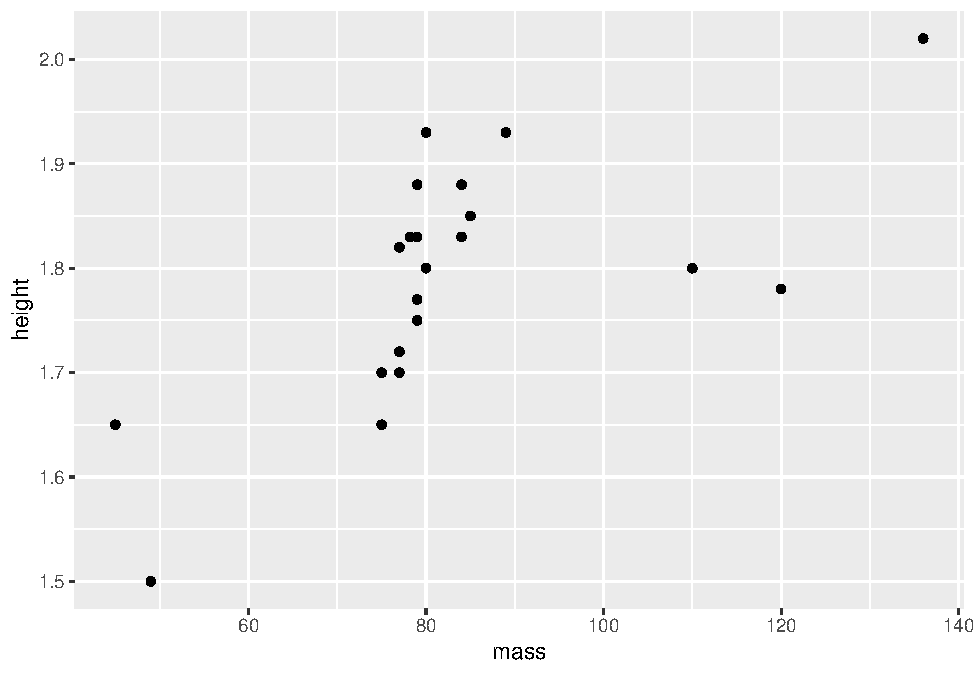
\includegraphics[width=0.75\linewidth,height=0.75\textheight]{02-Gestion_files/figure-latex/ggplotpoint-1} 

}

\caption{Diagramme de dispersion}\label{fig:ggplotpoint}
\end{figure}

Voici une liste d'exemples de différentes représentations géométriques.

\hypertarget{diagramme-de-dispersion}{%
\section{Diagramme de dispersion}\label{diagramme-de-dispersion}}

Pour réaliser un diagramme de dispersion, la fonction se nomme \texttt{geom\_point}. La cartographie identifie la variable à l'axe des \(x\) (horizontal) et des \(y\) (vertical). Dans cet exemple, il s'agit du poids (\(x\)) et de la taille (\(y\)). La cartographie ne se limite pas aux axes par contre. Dans cet exemple, la forme \texttt{shape} est aussi un dimension manipulée. Il aurait pu s'agir de \texttt{color} et même de \texttt{size}. Dans le code ci-dessous, \texttt{size} est placé à l'extérieur de \emph{mapping}, il s'agit alors d'une constante (elle change la taille des points), c'est-à-dire qu'elle ne varie pas avec les variables.

\begin{Shaded}
\begin{Highlighting}[]
\NormalTok{jd }\SpecialCharTok{\%\textgreater{}\%} 
  \FunctionTok{ggplot}\NormalTok{() }\SpecialCharTok{+} 
  \FunctionTok{geom\_point}\NormalTok{(}\AttributeTok{mapping =} \FunctionTok{aes}\NormalTok{(}\AttributeTok{x =}\NormalTok{ mass, }\AttributeTok{y =}\NormalTok{ height, }\AttributeTok{shape =}\NormalTok{ sex), }\AttributeTok{size =} \DecValTok{2}\NormalTok{) }
\end{Highlighting}
\end{Shaded}

\begin{figure}

{\centering 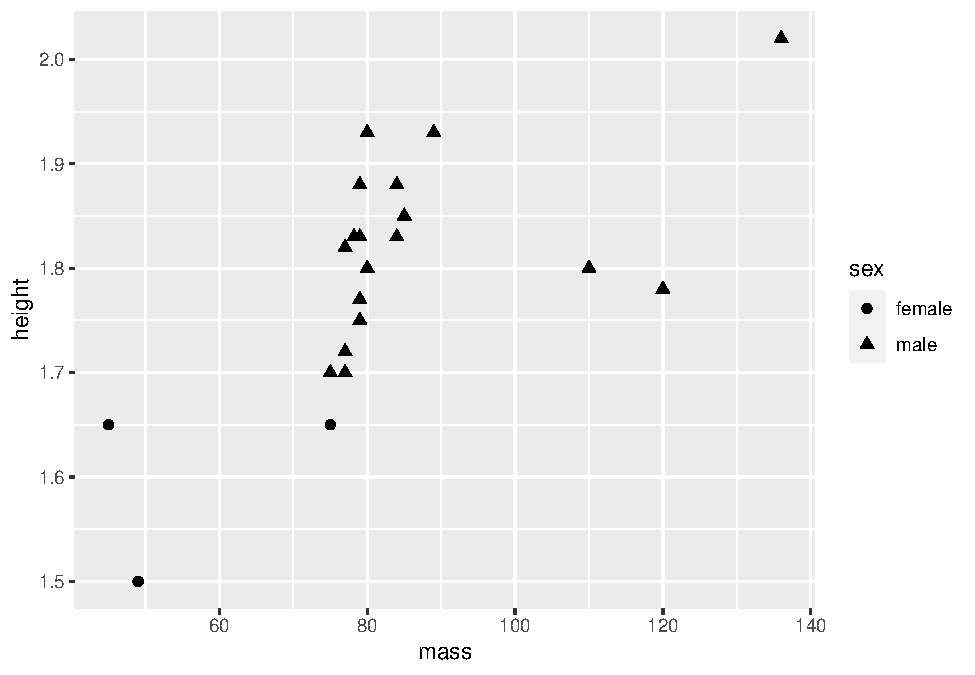
\includegraphics[width=0.75\linewidth,height=0.75\textheight]{02-Gestion_files/figure-latex/diagdisp-1} 

}

\caption{Le lien entre le poids et la taille en fonction du sexe}\label{fig:diagdisp}
\end{figure}

La figure \ref{fig:diagdisp2} montre le résultat si `size``est ajouté au \emph{mapping} pour identifier l'IMC. Les unités avec un plus grand IMC obtiennent un plus gros pointeur.

\begin{Shaded}
\begin{Highlighting}[]
\NormalTok{jd }\SpecialCharTok{\%\textgreater{}\%} 
  \FunctionTok{ggplot}\NormalTok{() }\SpecialCharTok{+} 
  \FunctionTok{geom\_point}\NormalTok{(}\AttributeTok{mapping =} \FunctionTok{aes}\NormalTok{(}\AttributeTok{x =}\NormalTok{ mass, }\AttributeTok{y =}\NormalTok{ height, }\AttributeTok{shape =}\NormalTok{ sex, }\AttributeTok{size =}\NormalTok{ IMC)) }
\end{Highlighting}
\end{Shaded}

\begin{figure}

{\centering 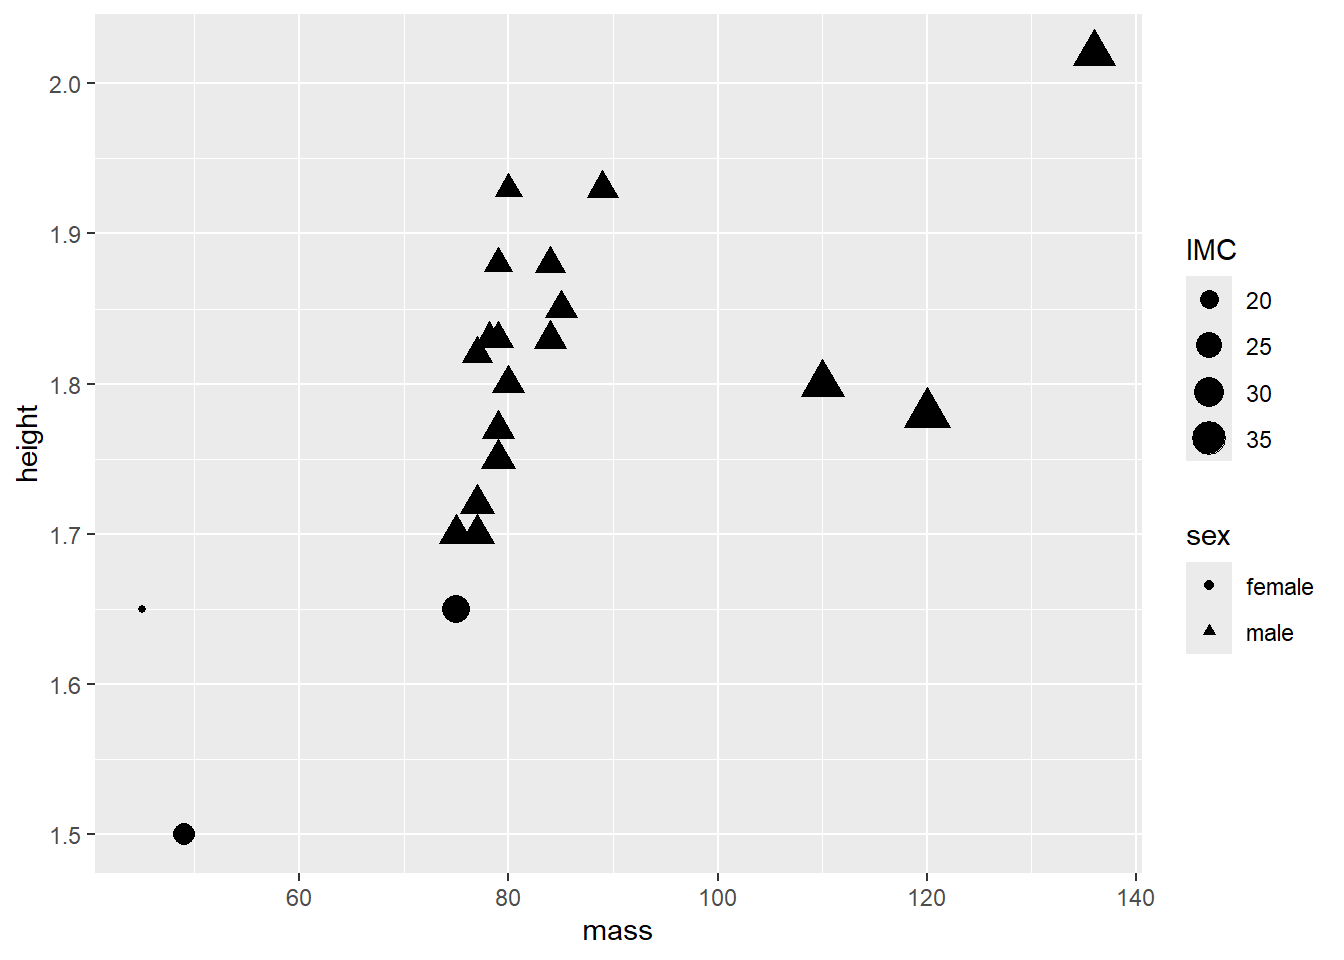
\includegraphics[width=0.75\linewidth,height=0.75\textheight]{02-Gestion_files/figure-latex/diagdisp2-1} 

}

\caption{Le lien entre le poids et la taille en fonction de l'IMC et du sexe}\label{fig:diagdisp2}
\end{figure}

On peut y ajouter la droite de régression, comme la Figure \ref{fig:diagdisp3} le montre. Ne pas ajouter \texttt{geom\_point()} ne ferait que produire la droite. Les arguments de \texttt{geom\_smooth()} indique que l'utilisation du modèle linéaire et l'absence des intervalles de confiance. Dans ce code, également comme le \emph{mapping} est ajouté à \texttt{ggplot} directement, il se généralise directement à \texttt{geom\_point()} et \texttt{geom\_smoooth()}

\begin{Shaded}
\begin{Highlighting}[]
\NormalTok{jd }\SpecialCharTok{\%\textgreater{}\%} 
  \FunctionTok{ggplot}\NormalTok{(}\AttributeTok{mapping =} \FunctionTok{aes}\NormalTok{(}\AttributeTok{x =}\NormalTok{ mass, }\AttributeTok{y =}\NormalTok{ height)) }\SpecialCharTok{+} 
  \FunctionTok{geom\_point}\NormalTok{(}\AttributeTok{size =} \DecValTok{2}\NormalTok{) }\SpecialCharTok{+}
  \FunctionTok{geom\_smooth}\NormalTok{(}\AttributeTok{method =}\NormalTok{ lm, }\AttributeTok{se =} \ConstantTok{FALSE}\NormalTok{, }\AttributeTok{color =} \StringTok{"black"}\NormalTok{)}
\CommentTok{\#\textgreater{} \textasciigrave{}geom\_smooth()\textasciigrave{} using formula \textquotesingle{}y \textasciitilde{} x\textquotesingle{}}
\end{Highlighting}
\end{Shaded}

\begin{figure}

{\centering 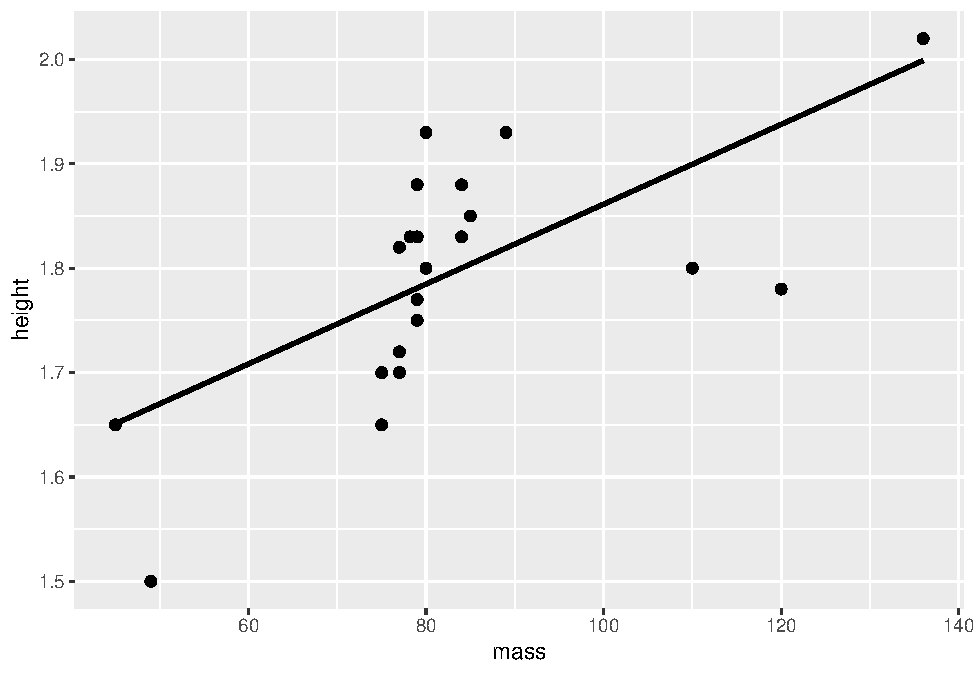
\includegraphics[width=0.75\linewidth,height=0.75\textheight]{02-Gestion_files/figure-latex/diagdisp3-1} 

}

\caption{Le lien entre le poids et la taille en fonction de l'IMC}\label{fig:diagdisp3}
\end{figure}

\hypertarget{bouxeete-uxe0-moustache}{%
\section{Boîte à moustache}\label{bouxeete-uxe0-moustache}}

La boîte à moustaches (\emph{box-and-whisker plot}) est une figure permettant de voir la variabilité des données. Elle résume seulement quelques indicateurs de position soit la médiane, les quartiles, le minimum, et le maximum. Ce diagramme est utilisé principalement pour détecter des valeurs aberrantes et comparer la variabilité entre les groupes. C'est la représentation géométrique \texttt{geom\_boxplot()} qui permettra de créer des boîtes à moustache. La cartographie prend en argument un variable nominale en \texttt{x} et une variable continue en \texttt{y}.

\begin{Shaded}
\begin{Highlighting}[]
\FunctionTok{ggplot}\NormalTok{(}\AttributeTok{data =}\NormalTok{ jd) }\SpecialCharTok{+} 
  \FunctionTok{geom\_boxplot}\NormalTok{(}\AttributeTok{mapping =} \FunctionTok{aes}\NormalTok{(}\AttributeTok{x =}\NormalTok{ sex, }\AttributeTok{y =}\NormalTok{ IMC)) }\SpecialCharTok{+}
  \FunctionTok{coord\_flip}\NormalTok{()}
\end{Highlighting}
\end{Shaded}

\begin{figure}

{\centering 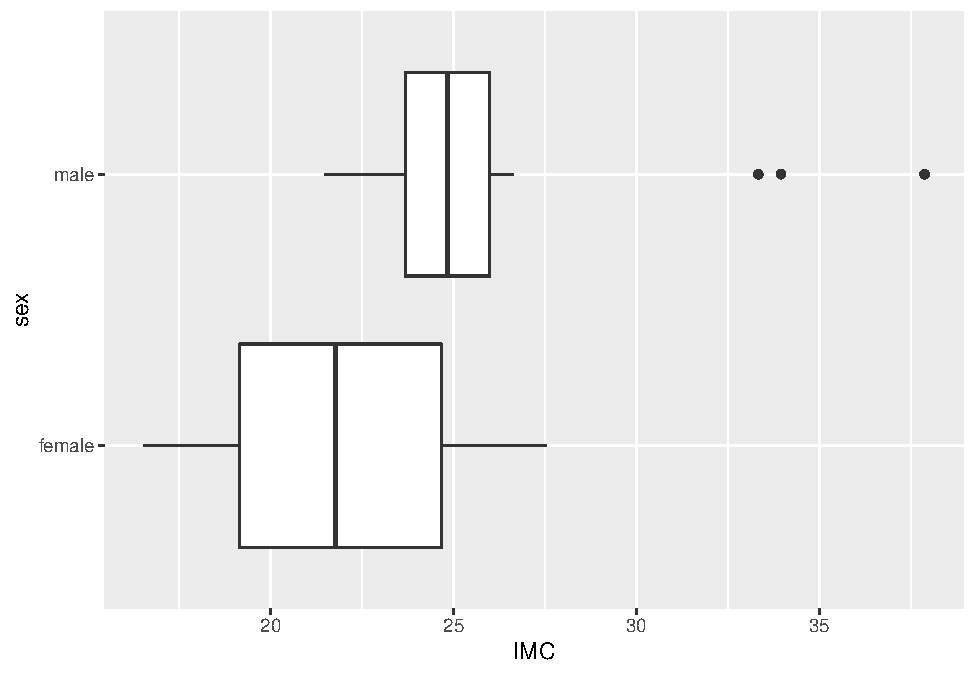
\includegraphics[width=0.75\linewidth,height=0.75\textheight]{02-Gestion_files/figure-latex/boxplot1-1} 

}

\caption{Boîte à moustache de l'IMC en fonction du sexe}\label{fig:boxplot1}
\end{figure}

Une fonction intéressante est la fonction \texttt{coord\_flip()} qui tourne (\emph{flip}) les axes, les coordonnées. L'axe \(x\) prend la place de \(y\); \(y\) prend la place de \(x\). Elle peut être pratique pour améliorer la qualité visuelle de certains graphiques.

\hypertarget{histogramme}{%
\section{Histogramme}\label{histogramme}}

Un histogramme permet de représenter la répartition empirique d'une variable. Il donne aperçu de la distribution sous-jacente, soit comment les données sont distribuées. Cette figure permet de voir la forme de la distribution et permet de voir si elle ne démontre pas d'anomalie. La représentation graphique \texttt{geom\_histogram()} produit des histogrammes. S'il faut en produire pour différentes variables, une statégie simple est les produire en série.

\begin{Shaded}
\begin{Highlighting}[]
\CommentTok{\# Trois histogrammes en trois figures}
\FunctionTok{ggplot}\NormalTok{(}\AttributeTok{data =}\NormalTok{ jd) }\SpecialCharTok{+} 
  \FunctionTok{geom\_histogram}\NormalTok{(}\AttributeTok{mapping =} \FunctionTok{aes}\NormalTok{(}\AttributeTok{x =}\NormalTok{ height))}

\FunctionTok{ggplot}\NormalTok{(}\AttributeTok{data =}\NormalTok{ jd) }\SpecialCharTok{+} 
  \FunctionTok{geom\_histogram}\NormalTok{(}\AttributeTok{mapping =} \FunctionTok{aes}\NormalTok{(}\AttributeTok{x =}\NormalTok{ mass))}

\FunctionTok{ggplot}\NormalTok{(}\AttributeTok{data =}\NormalTok{ jd) }\SpecialCharTok{+} 
  \FunctionTok{geom\_histogram}\NormalTok{(}\AttributeTok{mapping =} \FunctionTok{aes}\NormalTok{(}\AttributeTok{x =}\NormalTok{ IMC))}
\end{Highlighting}
\end{Shaded}

Des techniques plus avancées permettront de créer la Figure \ref{fig:hist} d'un seul coup.

\begin{Shaded}
\begin{Highlighting}[]
\CommentTok{\# Trois histogrammes en une seule figure}
\CommentTok{\# en optimisant avec le tidyverse}
\NormalTok{jd }\SpecialCharTok{\%\textgreater{}\%}
  \FunctionTok{keep}\NormalTok{(is.numeric) }\SpecialCharTok{\%\textgreater{}\%} 
  \FunctionTok{gather}\NormalTok{() }\SpecialCharTok{\%\textgreater{}\%} 
  \FunctionTok{ggplot}\NormalTok{(}\FunctionTok{aes}\NormalTok{(value)) }\SpecialCharTok{+}
  \FunctionTok{facet\_wrap}\NormalTok{(}\SpecialCharTok{\textasciitilde{}}\NormalTok{ key, }\AttributeTok{scales =} \StringTok{"free"}\NormalTok{) }\SpecialCharTok{+}
  \FunctionTok{geom\_histogram}\NormalTok{()}
\CommentTok{\#\textgreater{} \textasciigrave{}stat\_bin()\textasciigrave{} using \textasciigrave{}bins = 30\textasciigrave{}. Pick better value with}
\CommentTok{\#\textgreater{} \textasciigrave{}binwidth\textasciigrave{}.}
\end{Highlighting}
\end{Shaded}

\begin{figure}

{\centering 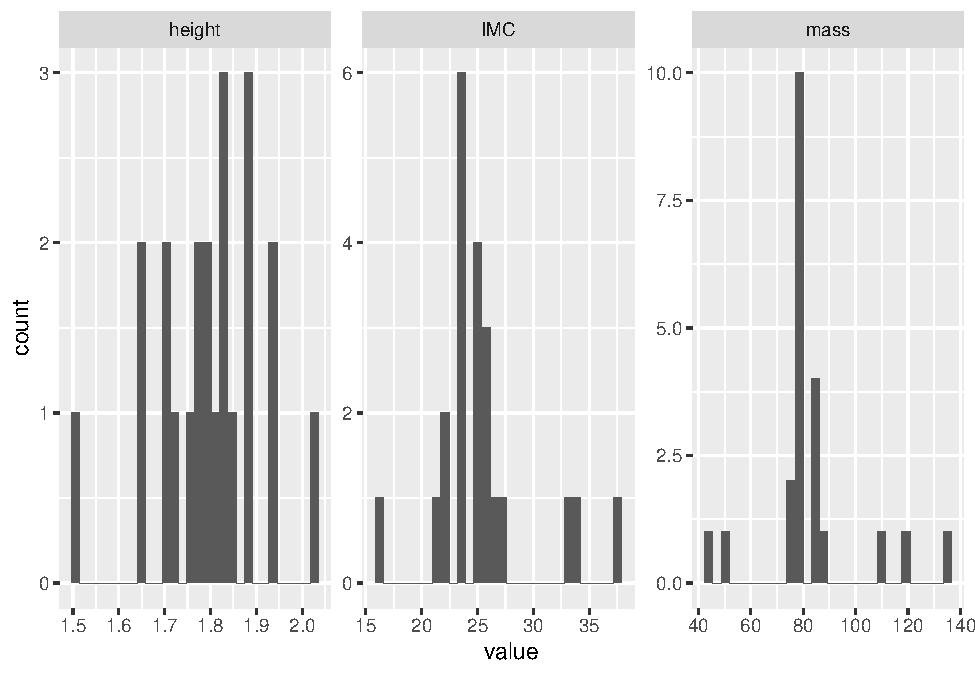
\includegraphics[width=0.75\linewidth,height=0.75\textheight]{02-Gestion_files/figure-latex/hist-1} 

}

\caption{Histogrammes des variables continues}\label{fig:hist}
\end{figure}

Enfin, s'il est désiré de comparer deux distributions de groupes différents, l'argument \texttt{fill} dans la cartographie indiquera à la fonction de différencier les valeurs selon le \emph{remplissage} des histogrammes.

\begin{Shaded}
\begin{Highlighting}[]
\NormalTok{jd }\SpecialCharTok{\%\textgreater{}\%} 
  \FunctionTok{ggplot}\NormalTok{(}\AttributeTok{mapping =} \FunctionTok{aes}\NormalTok{(}\AttributeTok{x =}\NormalTok{ IMC, }\AttributeTok{fill =}\NormalTok{ sex)) }\SpecialCharTok{+} 
  \FunctionTok{geom\_histogram}\NormalTok{(}\AttributeTok{position =} \StringTok{"identity"}\NormalTok{, }\AttributeTok{alpha =}\NormalTok{ .}\DecValTok{7}\NormalTok{) }\SpecialCharTok{+} 
  \FunctionTok{scale\_fill\_grey}\NormalTok{()}
\CommentTok{\#\textgreater{} \textasciigrave{}stat\_bin()\textasciigrave{} using \textasciigrave{}bins = 30\textasciigrave{}. Pick better value with}
\CommentTok{\#\textgreater{} \textasciigrave{}binwidth\textasciigrave{}.}
\end{Highlighting}
\end{Shaded}

\begin{figure}

{\centering \includegraphics[width=0.75\linewidth,height=0.75\textheight]{02-Gestion_files/figure-latex/hist2-1} 

}

\caption{Histogrammes de l'IMC par rapport au sexe}\label{fig:hist2}
\end{figure}

Dans la figure \ref{fig:hist2}, l'argument \texttt{position\ =\ "identity"} indique de traiter les deux groupes comme différents, autrement les colonnes s'additionneraient dans le graphique. L'argument \texttt{alpha\ =\ .7} permet une transparence entre les couleurs, autrement, les valeurs \emph{derrière} les autres ne paraîtraient pas. La valeur de \texttt{alpha} va de 0 (transparent) à 1 (opaque) et fonctionnera dans la plupart des contextes, surtout ceux liés à \texttt{ggplot2}.

\hypertarget{les-barres-derreurs}{%
\section{Les barres d'erreurs}\label{les-barres-derreurs}}

Les barres d'erreur sont une représentation géométrique à part entière. C'est une composante que l'on peut ajouter. La fonction pour les commandées est \texttt{geom\_errorbar()}. Elle nécessite deux arguments, soit l'intervalle de confiance maximale et minimale autour des moyennes à afficher.

La figure \ref{fig:erreurbar} illustre les différences entre moyennes avec des barres d'erreur à partir de la base de données \texttt{ToothGrowth}, une étude de l'effet de la vitamine C (\texttt{dose}) selon leur administration (jus ou supplément \texttt{supp}) sur la longueur des dents des cochons d'inde. Il y a deux facteurs et une variable continue.

La première étape est de tirer les statistiques sommaires, moyennes, écart type, tailles des groupes. La syntaxe tire profit de \texttt{groupe\_by()} pour tirer les groupes et en faire le sommaire. Le sommaire \texttt{summarise} permet d'obtenir les statistiques, notamment la moyenne, l'erreur standard (\texttt{se}) pour en calculer l'intervalle autour de la moyenne \texttt{ci}.

\begin{Shaded}
\begin{Highlighting}[]
\NormalTok{jd }\OtherTok{=}\NormalTok{ ToothGrowth }\SpecialCharTok{\%\textgreater{}\%} 
  \FunctionTok{group\_by}\NormalTok{(dose, supp) }\SpecialCharTok{\%\textgreater{}\%} 
  \FunctionTok{summarise}\NormalTok{(}\AttributeTok{mlen =} \FunctionTok{mean}\NormalTok{(len),}
            \AttributeTok{sdlen =} \FunctionTok{sd}\NormalTok{(len),}
            \AttributeTok{nlen =} \FunctionTok{n}\NormalTok{(), }
            \AttributeTok{se =} \FunctionTok{sd}\NormalTok{(len)}\SpecialCharTok{/}\FunctionTok{sqrt}\NormalTok{(}\FunctionTok{n}\NormalTok{()), }
            \AttributeTok{ci =} \FunctionTok{qt}\NormalTok{(.}\DecValTok{975}\NormalTok{, }\AttributeTok{df =} \FunctionTok{n}\NormalTok{()}\SpecialCharTok{{-}}\DecValTok{1}\NormalTok{) }\SpecialCharTok{*}\NormalTok{ se,}
            \AttributeTok{.groups =} \StringTok{"drop"}\NormalTok{)}

\NormalTok{jd }\SpecialCharTok{\%\textgreater{}\%} 
  \FunctionTok{ggplot}\NormalTok{(}\FunctionTok{aes}\NormalTok{(}\AttributeTok{x =}\NormalTok{ dose,}
             \AttributeTok{y =}\NormalTok{ mlen, }
             \AttributeTok{shape =}\NormalTok{ supp),}
         \AttributeTok{size =} \DecValTok{5}\NormalTok{) }\SpecialCharTok{+} 
    \FunctionTok{geom\_errorbar}\NormalTok{(}\FunctionTok{aes}\NormalTok{(}\AttributeTok{ymin =}\NormalTok{ mlen }\SpecialCharTok{{-}}\NormalTok{ ci,}
                      \AttributeTok{ymax =}\NormalTok{ mlen }\SpecialCharTok{+}\NormalTok{ ci), }
                  \AttributeTok{width =}\NormalTok{ .}\DecValTok{05}\NormalTok{) }\SpecialCharTok{+}
    \FunctionTok{geom\_line}\NormalTok{() }\SpecialCharTok{+}
    \FunctionTok{geom\_point}\NormalTok{()}
\end{Highlighting}
\end{Shaded}

\begin{figure}

{\centering 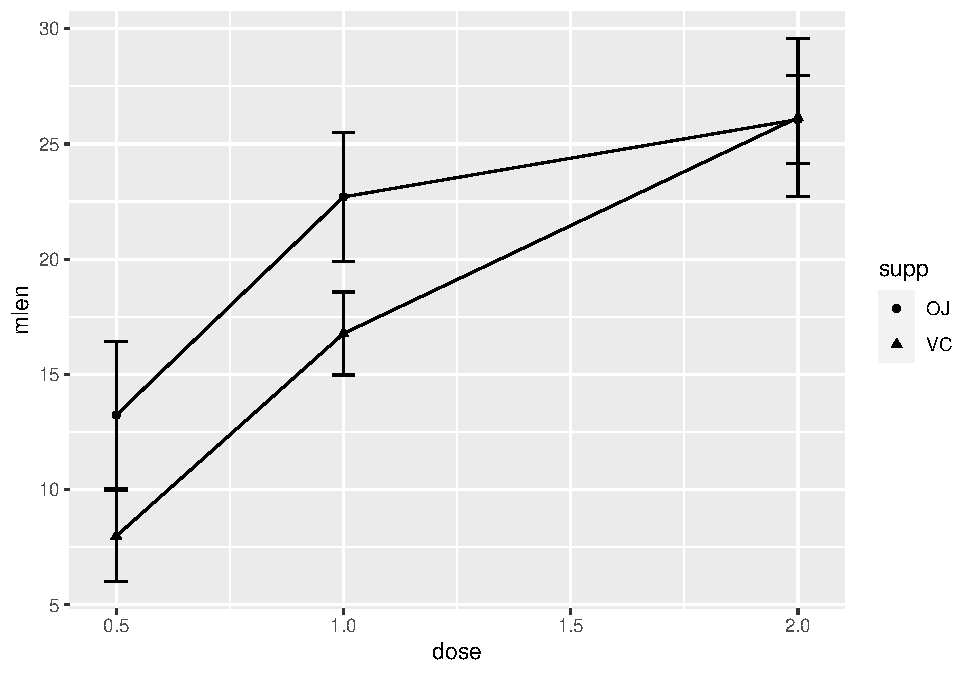
\includegraphics[width=0.75\linewidth,height=0.75\textheight]{02-Gestion_files/figure-latex/erreurbar-1} 

}

\caption{Les effets de la vitamine C sur les cochons d'inde}\label{fig:erreurbar}
\end{figure}

Une fois ces statistiques calculées et enregistrées dans le nouveau jeu de données \texttt{jd}, il est possible de créer le graphique avec les représentations géométriques désirées. Remarquer comment spécifié la cartographie dans le niveau \texttt{ggplot()} rend la syntaxe moins compliquée. Cette syntaxe produit un graphique avec \texttt{dose} à l' axe des \(x\), \texttt{supp} comme pointeurs et les moyennes de \texttt{len} (longueur moyenne des dents). La fonction \texttt{geom\_errorbar()} indique où placer les limites inférieures et supérieures des intervalles. Les arguments \texttt{size\ =\ 5} et \texttt{width\ =\ .05} sont ajoutés par pur esthétisme. L'argument \texttt{.groups\ =\ "drop"} de \texttt{summarise} permet d'éviter une avertissement expliquant qu'une variable de groupement est utilisé pour regrouper les résultats à la fin. Ajouter ou retirer cet argument ne change pas les calculs.

\hypertarget{pour-aller-plus-loin}{%
\section{Pour aller plus loin}\label{pour-aller-plus-loin}}

Il existe une multitudes de livres, de sites web, de tutoriels en ligne et d'atelier pour donner l'occasion au lecteur d'aller plus loin dans sa conception graphique. Voici quelques ouvrages de références : Le \emph{R Graphics Cookbook} (Chang) repérable à \url{https://r-graphics.org/}, \emph{ggplot2: elegant graphics for data analysis} (Wickham) repérable à \url{https://ggplot2-book.org/} ou \emph{R Graphics} (Murrel) repérable à \url{https://www.stat.auckland.ac.nz/~paul/RG2e/}.

\hypertarget{exercice-gestion}{%
\chapter*{Exercices}\label{exercice-gestion}}
\addcontentsline{toc}{chapter}{Exercices}

\begin{enumerate}
\def\labelenumi{\arabic{enumi}.}
\item
  Prendre le jeu de données \texttt{mtcars} et produire un diagramme de dispersion montrant la puissance brute (en chevaux) (\texttt{hp}) par rapport à consommation en km/l (basé sur \texttt{mpg}) tout en soulignant l'effet du nombre de cylindres (\texttt{cyl}). \textbf{Attention} la fonction \texttt{as\_factor} permettra d'utiliser \texttt{cyl} en facteur.
\item
  Prendre le jeu de données \texttt{mtcars} et produire un histogramme montrant la variabilité de la consommation \texttt{mpg} par rapport à la transmission (\texttt{am}). \textbf{Attention} la fonction \texttt{as\_factor} permettra d'utiliser \texttt{am} en facteur.
\item
  Prendre le jeu de données \texttt{msleep} et produire un diagramme à bâton pour observer la fréquence de différents type de régime (\texttt{vore}). \textbf{Attention} aux données manquantes.
\item
  Prendre le jeu de données \texttt{msleep} et produire une boîte à moustache pour observer le temps total de sommeil (\texttt{sleep\_total}) par rapport aux régimes (\texttt{vore}). \textbf{Attention} aux données manquantes.
\end{enumerate}

\hypertarget{part-analyses-statistiques}{%
\part{Analyses statistiques}\label{part-analyses-statistiques}}

\hypertarget{infuxe9rer}{%
\chapter{Inférer}\label{infuxe9rer}}

Le but principal de toute inférence statistique est de tirer des conclusions sur une population à partir d'un échantillon (un fragment beaucoup plus petit de la population). Avant d'introduire différents tests statistiques permettant de tirer ce genre de conclusions, le théorème central limite et la théorie des tests d'hypothèses seront présentés. La distribution centrale réduite (score-\(z\)) et la distribution-\(t\) serviront d'appui à la présentation.

Comme il est rarement possible de collecter des données sur l'ensemble de la population, l'expérimentateur choisi, idéalement, un échantillon représentatif tiré aléatoirement. Une fois l'échantillon recruté et mesuré, l'expérimentateur dérive des indices statistiques. Un \textbf{indice} statistique synthétise par une estimation basée sur l'échantillon de l'information sur le \textbf{paramètre} de la population. Cet indice possède un comportement, une distribution d'échantillonnage qui détermine les différentes valeurs qu'il peut prendre. En obtenant ces indices, l'expérimentateur tente de connaître le paramètre de la population. S'il s'intéresse à la relation entre l'anxiété et un cours de méthodes quantitatives, l'expérimentateur voudra savoir d'une part si cette relation n'est pas nulle, mais aussi sa force, en termes de tailles d'effet.

Cette tâche peut apparaître difficile considérant le peu d'informations sur la population, sa distribution de probabilité, les paramètres et la relative petite taille de l'échantillon par rapport à la population. Pour aider l'expérimentateur, les statisticiens ont le théorème central limite. Pour eux, il est certainement l'équivalent de la théorie de l'évolution pour le biologiste ou la théorie de la relativité générale pour le physicien. Ce théorème permet de connaître comment et sous quelles conditions se comportent les variables aléatoires.

\hypertarget{le-thuxe9oruxe8me-central-limite}{%
\section{Le théorème central limite}\label{le-thuxe9oruxe8me-central-limite}}

Les valeurs d'un échantillon sont, pour le statisticien, des variables aléatoires. Une variable aléatoire, c'est un peu comme piger dans une boîte à l'aveuglette pour obtenir une valeur. La boîte est impénétrable, personne ne sait par quel processus elle accorde telle ou telle autre valeur. Pour le statisticien, ce qui importe c'est que chaque valeur possède une chance égale aux autres d'être sélectionnée et qu'elles soient indépendantes entre elles (le fait d'en choisir une soit sans conséquence sur la probabilité des autres). Pour le non-initié aux fonctions permettant de créer des nombres pseudoaléatoires, une fonction \textbf{R} comme \texttt{rnorm()} ou \texttt{runif()} (\emph{r} suivi d'un nom de distribution, voir \protect\hyperlink{les-distributions}{Les distributions}) joue parfaitement le rôle de cette boîte. Si l'usager demande une valeur, la fonction retourne une valeur aléatoire (imprévisible à chaque fois) sans connaître comment cette valeur est produite.

\begin{Shaded}
\begin{Highlighting}[]
\FunctionTok{runif}\NormalTok{(}\AttributeTok{n =} \DecValTok{1}\NormalTok{)}
\CommentTok{\#\textgreater{} [1] 0.52}
\end{Highlighting}
\end{Shaded}

Le statisticien s'intéresse à inférer comment ces valeurs sont générées. Il postule ainsi que les valeurs aléatoires suivent une distribution de probabilité. Connaître cette distribution est très important, car c'est elle qui permet de répondre à des questions comme : quelle est la probabilité d'obtenir un résultat aussi rare que \(x\)? Ou quelle sont les valeurs attendues pour \(95\%\) des tirages? Questions tout à fait pertinentes pour l'expérimentateur. Une des distributions les plus connues est certainement la distribution normale, celle qui est derrière la fonction \texttt{rnorm()} d'ailleurs. Mais, il y en a beaucoup, beaucoup d'autres.

Lorsque plus d'une variable sont issues d'une même boîte (distribution), elles sont \emph{identiquement distribuées}. Si ces variables aléatoires sont combinées, que ce soit en termes de produit, de quotient, d'addition, de soustraction, le résultat est une nouvelle variable aléatoire qui possède sa propre distribution nommée \emph{distribution d'échantillonnage}. Sur le plan de la syntaxe \textbf{R}, il s'agit de réaliser des opérations mathématiques avec des variables aléatoires identiquement distribuées.

\begin{Shaded}
\begin{Highlighting}[]
\CommentTok{\# Pour répliquer}
\FunctionTok{set.seed}\NormalTok{(}\DecValTok{1}\NormalTok{)}

\CommentTok{\# Création de deux variables identiquement distribuées}
\NormalTok{a }\OtherTok{\textless{}{-}} \FunctionTok{runif}\NormalTok{(}\AttributeTok{n =} \DecValTok{1}\NormalTok{)}
\NormalTok{b }\OtherTok{\textless{}{-}} \FunctionTok{runif}\NormalTok{(}\AttributeTok{n =} \DecValTok{1}\NormalTok{)}
\NormalTok{a ; b}
\CommentTok{\#\textgreater{} [1] 0.266}
\CommentTok{\#\textgreater{} [1] 0.372}

\CommentTok{\# Une nouvelle variable aléatoire}
\NormalTok{total }\OtherTok{\textless{}{-}}\NormalTok{ a }\SpecialCharTok{+}\NormalTok{ b}
\end{Highlighting}
\end{Shaded}

Entre en jeu le \emph{théorème central limite}: plus des variables aléatoires identiquement distribuées sont additionnées ensemble, plus la distribution de probabilité de cette somme se rapproche d'une distribution normale.

Par exemple, la fonction \texttt{rlnorm()} génère des variables issues d'une distribution log normale. Elle a la forme illustré à la Figure \ref{fig:lognormal} (qui n'a rien de normal à première vue).

\begin{figure}

{\centering 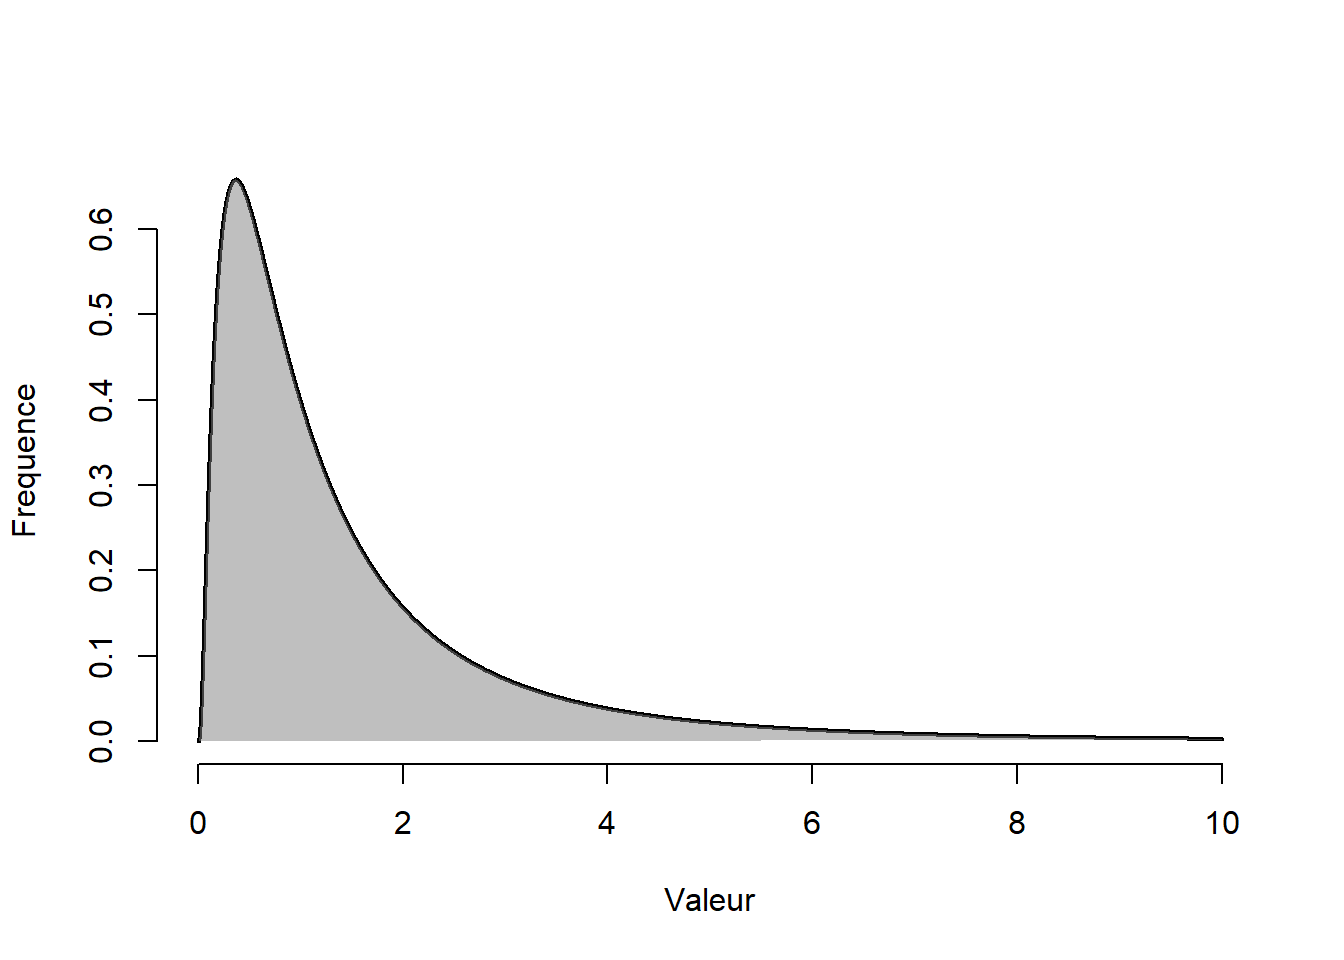
\includegraphics[width=0.8\linewidth,height=0.8\textheight]{03-Inferences_files/figure-latex/lognormal-1} 

}

\caption{Distribution log normale}\label{fig:lognormal}
\end{figure}

En calculant la somme de plusieurs variables aléatoires de cette distribution, pour diverses valeurs de tailles d'échantillons (nombre de variables échantillonnées), les résultats tendent de plus en plus vers une distribution normale. Le code ci-dessous présente la démarche utilisée et la figure \ref{fig:testn} en fait la démonstration graphique en présentant les distributions d'échantillonnage obtenues.

\begin{Shaded}
\begin{Highlighting}[]
\CommentTok{\# Cette fonction sort les nombres, mais pas les graphiques.}
\CommentTok{\# Différentes tailles d\textquotesingle{}échantillons}
\NormalTok{N }\OtherTok{=} \FunctionTok{seq}\NormalTok{(}\DecValTok{10}\NormalTok{, }\DecValTok{90}\NormalTok{, }\AttributeTok{by =} \DecValTok{10}\NormalTok{)}
\CommentTok{\# Nombre de tirage pour chaque élément de N}
\NormalTok{reps }\OtherTok{=} \DecValTok{1000}

\CommentTok{\# Une boucle pour tester toutes les possibilités}
\ControlFlowTok{for}\NormalTok{(n }\ControlFlowTok{in}\NormalTok{ N)\{}
\NormalTok{  total }\OtherTok{=} \FunctionTok{as.numeric}\NormalTok{()}
  \ControlFlowTok{for}\NormalTok{(i }\ControlFlowTok{in} \DecValTok{1}\SpecialCharTok{:}\NormalTok{reps)\{}
    \CommentTok{\# Faire la somme de n valeurs tirés d\textquotesingle{}une distribution log normale}
\NormalTok{    total[i] }\OtherTok{=} \FunctionTok{sum}\NormalTok{(}\FunctionTok{rlnorm}\NormalTok{(n))}
\NormalTok{  \}}
  \CommentTok{\# hist(total) }
\NormalTok{\}}
\end{Highlighting}
\end{Shaded}

La Figure \ref{fig:testn} montre que la distribution d'échantillonnage de la somme des variables converge vers une distribution normale à mesure que la taille d'échantillon \(n\) augmente. Cela est vrai pour n'importe quelle distribution de probabilité de la population. Le théorème central en dit plus que simplement la forme de la distribution. Elle affirme également qu'une distribution de probabilité d'une population ayant une moyenne \(\mu\) et un écart type \(\sigma\) échantillonnées sur \(n\) unités, générera une distribution d'échantillonnage des totaux (indicé \(t\)) ayant une espérance (la moyenne) de \(n\mu_t\) et un écart type de \(n\sigma_t^2\).

\begin{figure}
\centering
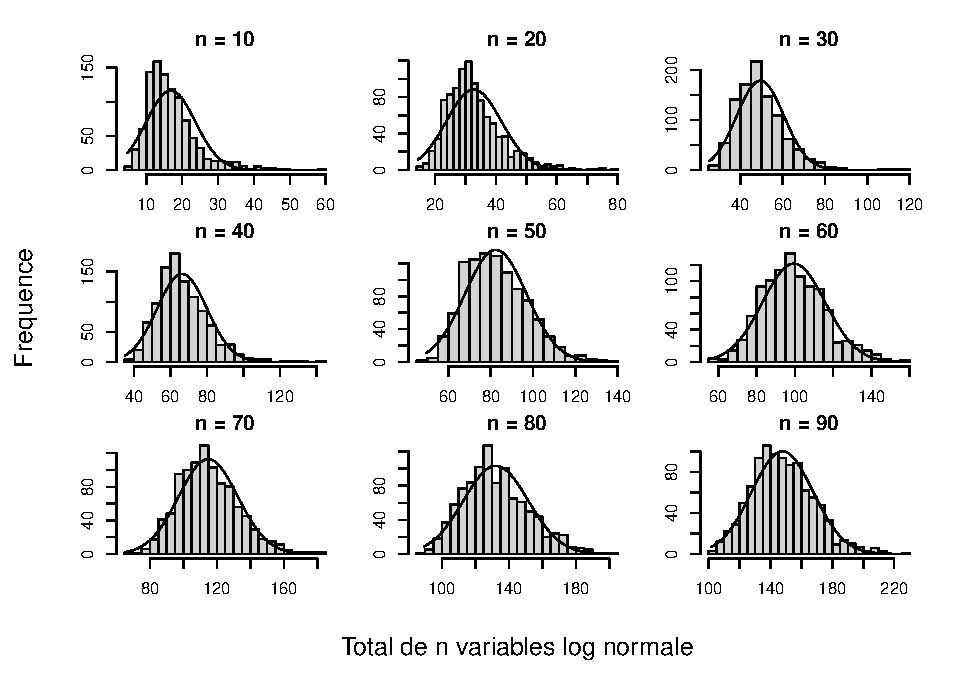
\includegraphics{03-Inferences_files/figure-latex/testn-1.pdf}
\caption{\label{fig:testn}Distributions des totaux de n variables log normales}
\end{figure}

Les expérimentateurs ne connaissent pas les distributions sous-jacentes aux valeurs des unités issues de la population. Par contre, à l'aide des statisticiens et du théorème central limite, ils savent comment se comportent les sommes des variables. Les expérimentateurs s'intéressent toutefois rarement aux sommes de variable\ldots{} à l'exception de la moyenne qui est une somme de variable divisée par la constante \(n\)\footnote{Ou encore la variance qui est la somme des écarts au carré. Les expérimentateurs s'intéressent aux sommes de variables en fait.}. Dans le cas de la moyenne, le théorème central limite stipule qu'une distribution de probabilité ayant une moyenne \(\mu\) et un écart type \(\sigma\) dont l'échantillon est constitué de \(n\) unités, générera une distribution d'échantillonnage des moyennes avec une espérance de \(\mu_{\bar{x}}\) et un écart type de \(\sigma_{\bar{x}}/\sqrt{n}\).

Dans la mesure où l'expérimentateur connaît la distribution de la population (extrêmement rare, mais permet de mieux illustrer la théorie) ou qu'il peut recourir à une distribution d'échantillonnage connue, il pourra inférer la probabilité d'une variable aléatoire par rapport à ce qui est attendu simplement par hasard. Il pourra alors juger si cette variable est trop rare par rapport à l'hypothèse de base (nulle).

La théorie traditionnelle des tests d'hypothèses repose sur l'idée selon laquelle on compare la vraisemblance d'une variable aléatoire estimée auprès d'un échantillon par rapport à une hypothèse nulle (l'absence d'effet). En épistémologie des sciences, il n'est pas possible de montrer l'exactitude d'une hypothèse, seulement son inexactitude. Cela rappelle le principe du falsificationnisme selon lequel on ne peut prouver une hypothèse, on ne peut que la falsifier. En statistiques, c'est la rareté d'une donnée qui agira comme indice d'\emph{inexactitude}. Si la variable aléatoire est trop rare pour l'hypothèse nulle, celle-ci est rejetée : d'autres hypothèses doivent être considérées pour expliquer ce résultat. Autrement, l'hypothèse nulle n'est pas rejetée, les preuves sont insuffisantes pour informer l'expérimentateur sur l'hypothèse nulle.

\hypertarget{infuxe9rence-avec-la-distribution-normale-sur-une-unituxe9}{%
\section{Inférence avec la distribution normale sur une unité}\label{infuxe9rence-avec-la-distribution-normale-sur-une-unituxe9}}

Un excellent exemple en sciences humaines et sociales où la distribution de probabilité de la population est connue est le quotient intellectuel (QI). Le QI d'une population occidentale est distribué normalement (établi intentionnellement par les psychométriciens) avec une moyenne de 100 (\(\mu=100\)) et un écart type de \(\sigma = 15\). Ces valeurs sont totalement arbitraires, il est tout aussi convenable de parler d'une moyenne de 0 et d'un écart type de 1 (la distribution pourrait être standardisée) quoiqu'il est contre-intuitif de parle d'un QI de 0. (Qui voudrait avoir une intelligence de 0?)

Dans la population, bien que la moyenne et la variance peuvent être connues, sélectionner une unité au hasard génère une variable aléatoire. Chaque individu de la population a une probabilité très faible d'être sélectionné et est indépendant des autres individus de la population. Il est très difficile de prédire le score exact d'une personne. Toutefois, il est possible d'avoir un idée de la variabilité des scores. La Figure \ref{fig:regle} montre la distribution normale par rapport à la moyenne, \(\mu\) pour différentes valeurs d'écart type, \(\sigma\). Elle montre que 68.269\% devrait se retrouvé entre plus ou moins un écart types ou encore que 95.45\% devrait se retrouvé entre plus ou moins deux écarts types. Ajuster au QI, il s'agit de 85 à 115 et de 70 à 130 respectivement

\begin{figure}

{\centering 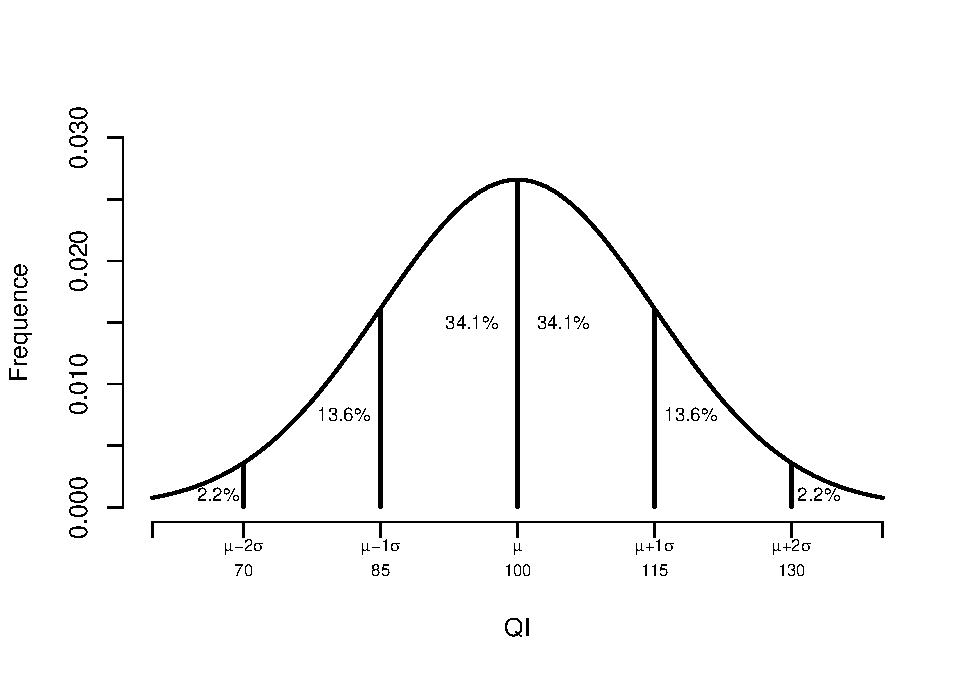
\includegraphics[width=0.9\linewidth,height=0.9\textheight]{03-Inferences_files/figure-latex/regle-1} 

}

\caption{La distribution normale du QI}\label{fig:regle}
\end{figure}

Une autre façon de fonctionner est de prendre une personne au hasard et de mesurer son QI. Le score obtenu est une valeur aléatoire. Comme la distribution est connue avec ses paramètres, il est possible de juger de la vraisemblance de ce score (est-il rare?) par rapport à la population.

Voici un exemple où ces informations sont pertinentes. Un groupe d'\emph{expérimentateurs} mettent en place un outil d'évaluation qui teste si un individu donné est un humain ou un reptilien (une race d'extra-terrestre). Leur outil n'est pas si sophistiqué. En fait, il se base sur le QI, car les expérimentateurs ont remarqué que les reptiliens ont un QI beaucoup plus élevé que le QI humain.

\begin{figure}
\centering
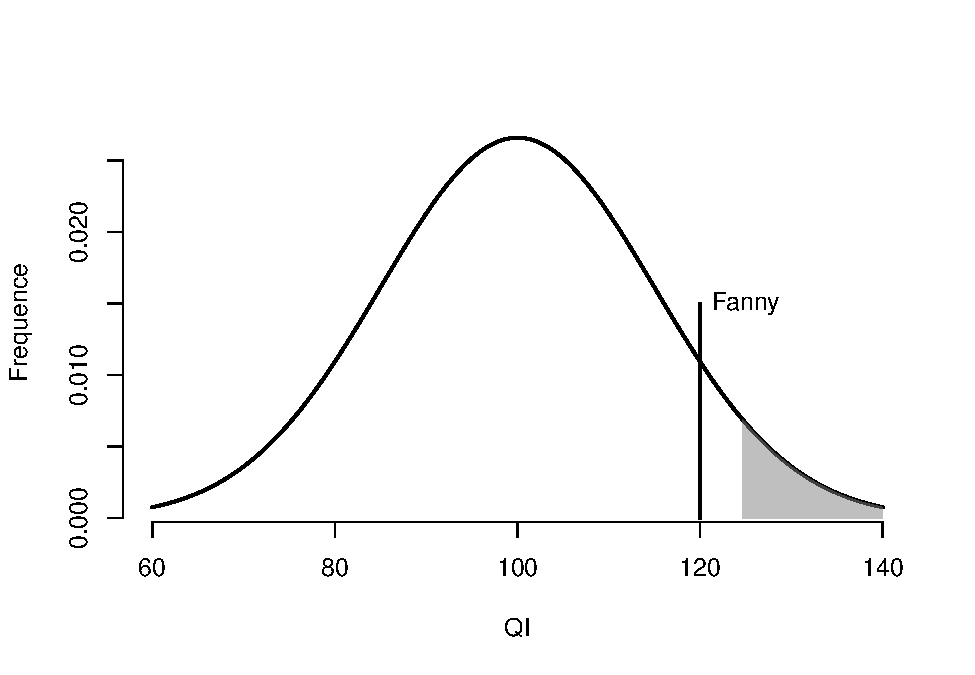
\includegraphics{03-Inferences_files/figure-latex/unnamed-chunk-5-1.pdf}
\caption{\label{fig:unnamed-chunk-5}Score de Fanny sur la distribution normale}
\end{figure}

La distribution normale du QI humain joue le rôle d'hypothèse nulle, les personnes mesurées sont admises humaines jusqu'à preuve du contraire (une présomption d'innocence en quelque sorte), un QI \emph{trop} élevé suggérant la culpabilité.

Les expérimentateurs émettent l'hypothèse que les 5 \% personnes ayant le plus haut QI sont vraisemblablement reptiliens. C'est le risque qu'ils sont prêts à prendre de sélectionner un humain et de le classer erronément comme reptilien.

Le groupe d'expérimentateurs teste leur instrument sur Fanny. Elle a un QI de 120. Comment tester si elle est reptilienne? La première étape est d'obtenir un score-\(z\). Un score-\(z\) est une échelle standardisée des distances d'une valeur par rapport à la moyenne. Lorsqu'une échelle de mesure est transformée en score-\(z\), la moyenne est de 0 et l'écart type est égal à 1. Cela permet de mieux apprécier les distances et leur probabilité. La Figure \ref{fig:regle} est ainsi applicable pour toutes sortes de situations où la distribution est vraisemblablement normale.

\begin{Shaded}
\begin{Highlighting}[]
\NormalTok{fanny }\OtherTok{\textless{}{-}} \DecValTok{120}
\NormalTok{z.fanny }\OtherTok{\textless{}{-}}\NormalTok{ (fanny }\SpecialCharTok{{-}} \DecValTok{100}\NormalTok{) }\SpecialCharTok{/} \DecValTok{15}
\end{Highlighting}
\end{Shaded}

Fanny a un score-\(z\) de 1.333. Maintenant, il faut traduire cette valeur en probabilité.

\begin{Shaded}
\begin{Highlighting}[]
\CommentTok{\# La probabilité que Fanny ait un QI de {-}Inf à z.fanny}
\FunctionTok{pnorm}\NormalTok{(z.fanny)}
\CommentTok{\#\textgreater{} [1] 0.909}
\end{Highlighting}
\end{Shaded}

L'expectative sous l'hypothèse nulle est d'observer un score pareil ou supérieur à celui de Fanny 9.121 \% du temps. Cette statistique correspond à la \emph{valeur-\(p\)}, la probabilité de l'indice par rapport à sa distribution d'échantillonnage (hypothèse nulle). Comme elle ne dépasse pas le seuil de 5\%, soit la limite selon laquelle le score est jugé invraisemblable, l'hypothèse nulle n'est pas rejetée (elle est humaine!).

Avec le critère d'identifier erronément les 5\% humains les plus intelligents, il s'agit, du même coup, du \textbf{taux de faux positif} \emph{acceptable} de l'étude. Un faible sacrifice à réaliser afin identifier des reptiliens parmi les humains. La zone de rejet, c'est-à-dire la zone dans laquelle l'hypothèse nulle (humain) est rejetée, correspond à la zone ombragée à droite de la distribution.

La logique des tests statistiques inférentiels repose sur cette série d'étapes : choisir un indice, connaître sa distribution sous-jacente, déterminer l'hypothèse nulle (généralement l'absence d'effet), calculer la probabilité de l'indice par rapport à cette hypothèse nulle.

\hypertarget{infuxe9rence-avec-la-distribution-normale-sur-un-uxe9chantillon}{%
\section{Inférence avec la distribution normale sur un échantillon}\label{infuxe9rence-avec-la-distribution-normale-sur-un-uxe9chantillon}}

Jusqu'à maintenant, seule une unité d'observation était traitée. L'indice et la distribution étaient également spécifiés. Dans cette section, l'exemple est étendu aux échantillons (plus d'une unité d'observation).

Fanny a un QI de 120. Si une autre personne avait été sélectionnée, cette nouvelle personne aurait inévitablement un autre score. Cette logique s'applique également aux échantillons. L'exemple ci-dessous échantillonne 10 unités d'une population de QI distribuée normalement avec les paramètres usuels.

\begin{Shaded}
\begin{Highlighting}[]
\CommentTok{\# Création d\textquotesingle{}un échantillon de 10 unités}
\FunctionTok{set.seed}\NormalTok{(}\DecValTok{824}\NormalTok{)}

\CommentTok{\# Dix valeurs arrondies avec une moyenne de 100 et un écart type de 10}
\NormalTok{QI }\OtherTok{\textless{}{-}} \FunctionTok{round}\NormalTok{(}\FunctionTok{rnorm}\NormalTok{(}\AttributeTok{n =} \DecValTok{10}\NormalTok{, }\AttributeTok{mean =} \DecValTok{100}\NormalTok{, }\AttributeTok{sd =} \DecValTok{15}\NormalTok{))}
\NormalTok{QI}
\CommentTok{\#\textgreater{}  [1] 110 111 102  99 109 102  99 110 132 114}
\end{Highlighting}
\end{Shaded}

\begin{figure}
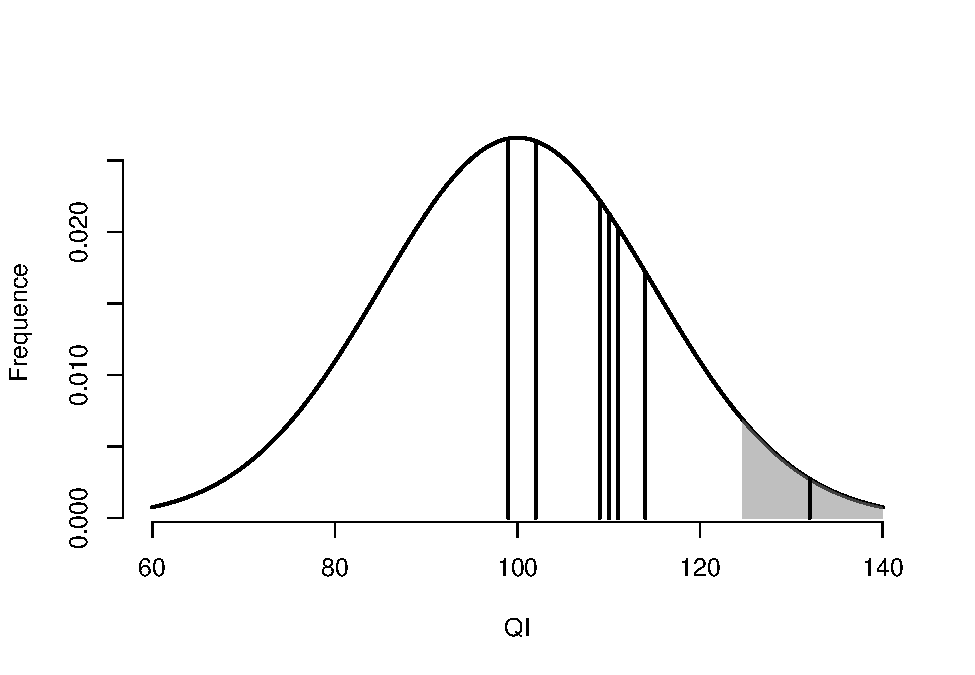
\includegraphics[width=0.9\linewidth,height=0.9\textheight]{03-Inferences_files/figure-latex/rept-1} \caption{Scores des unités de l'échantillon}\label{fig:rept}
\end{figure}

Dans la Figure \ref{fig:rept}, chaque unité est présentée par un trait vertical noir. La moyenne de cet échantillon est de 108.8 et l'écart type est de 9.762. Dans cet exemple, l'indice est clairement identifié, mais quelle est la distribution d'échantillonnage des moyennes? Selon le théorème central limite, la moyenne de la distribution d'échantillonnage est \(\mu=\mu_{\bar{x}}=100\) et l'écart type est \(\sigma_{\bar{x}} = \frac{\sigma}{\sqrt{n}}=\frac{15}{\sqrt{10}}=4.743\) . Maintenant, il est possible de calculer un score-\(z\).

\[
z = \frac{\bar{x}-\mu_{\bar{x}}}{\sigma/\sqrt{n}}=\frac{108.8-100}{15/\sqrt{10}}=1.855
\]
Cela donne le code suivant.

\begin{Shaded}
\begin{Highlighting}[]
\NormalTok{z }\OtherTok{\textless{}{-}}\NormalTok{ (}\FunctionTok{mean}\NormalTok{(QI) }\SpecialCharTok{{-}} \DecValTok{100}\NormalTok{)}\SpecialCharTok{/}\NormalTok{(}\DecValTok{15} \SpecialCharTok{/} \FunctionTok{sqrt}\NormalTok{(}\DecValTok{10}\NormalTok{))}
\NormalTok{z}
\CommentTok{\#\textgreater{} [1] 1.86}
\end{Highlighting}
\end{Shaded}

La fonction \texttt{(1\ -\ pnorm(z))\ *\ 100}, retourne la probabilité (en pourcentage) d'un résultat plus rare que l'indice obtenu auprès de l'échantillon par rapport à la population. Comme pour l'exemple de Fanny, ce chiffre est une valeur-\(p\), soit la probabilité de l'indice observé par rapport à l'hypothèse nulle. La probabilité de cet échantillon par rapport à l'hypothèse nulle est de 3.178\%, juste en deçà du 5\% fixé. La conclusion est par conséquent de rejeter l'hypothèse nulle, l'échantillon semble provenir d'une autre distribution (avec des paramètres différents) que celle postulée.

\begin{figure}
\centering
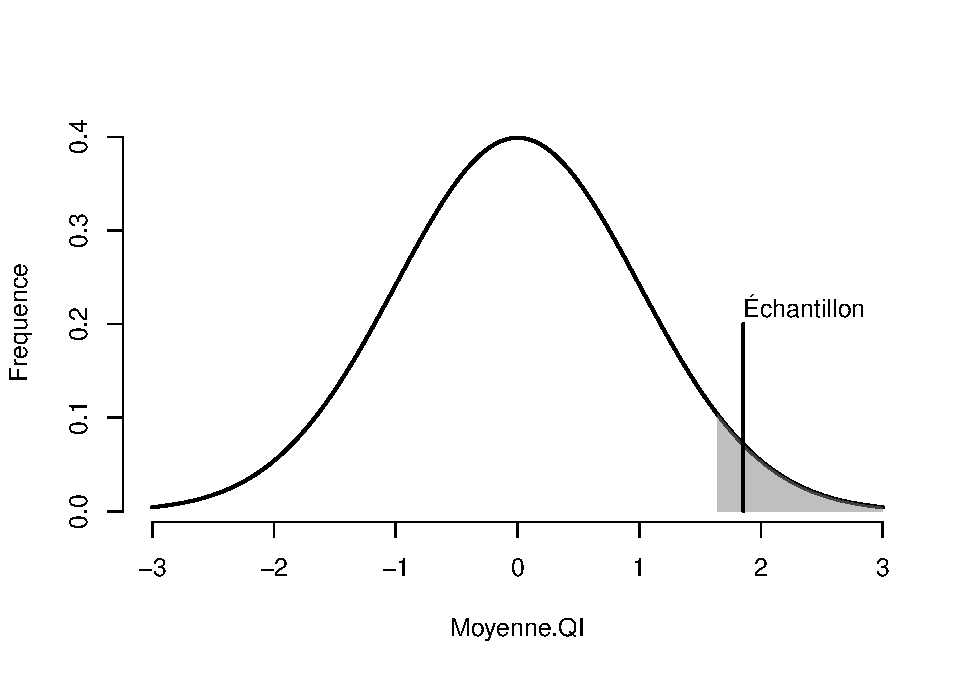
\includegraphics{03-Inferences_files/figure-latex/unnamed-chunk-10-1.pdf}
\caption{\label{fig:unnamed-chunk-10}Moyenne de l'échantillon sur la distribution normale}
\end{figure}

\textbf{Qu'en est-il vraiment de ce résultat?} Pour l'expérimentateur, il ne peut aller plus loin, car il ne connaît pas la boîte noire selon laquelle les valeurs de l'échantillon sont générées. Il ne peut que constater que plusieurs (9/10) unités ont un score plus élevé que 100. Par contre, comme il s'agit d'un exemple simulé, la boîte noire est connue. C'est la fonction, \texttt{round(rnorm(n\ =\ 10,\ mean\ =\ 100,\ sd\ =\ 15))}, une distribution normale ayant \(\mu=100,\sigma=15\) qui est utilisée pour générer les valeurs. L'utilisateur sait qu'il s'agit d'un faux positif (une erreur de Type I) : l'échantillon fait partie des 5\% des échantillons qui risquent de se faire rejeter accidentellement. Si l'utilisateur utilise une autre graine (\texttt{seed()}), il verra que la plupart (95\%) des moyennes ne seront pas rejetées.

Pour l'instant, seule une boîte noire a été examinée - celle de l'hypothèse nulle. Qu'advient-il du vrai phénomène? Par exemple, si les reptiliens existaient vraiment. Comme l'utilisateur est le maître du modèle, il peut spécifier les paramètres à sa convenance. Le QI des reptiliens pourraient être distribué comme une distribution normale ayant \(\mu_{r}=130, \sigma_r = 15\) où l'indice \(r\) ne fait qu'indiquer qu'il s'agit des paramètres de la population reptilienne. Les paramètres humains seront désignés par \(h\), soit \(\mu_h = 100,\sigma_h = 15\).

\begin{Shaded}
\begin{Highlighting}[]
\NormalTok{mu.h }\OtherTok{\textless{}{-}} \DecValTok{100}\NormalTok{ ; sd.h }\OtherTok{\textless{}{-}} \DecValTok{15}
\NormalTok{mu.r }\OtherTok{\textless{}{-}} \DecValTok{130}\NormalTok{ ; sd.r }\OtherTok{\textless{}{-}} \DecValTok{15}
\end{Highlighting}
\end{Shaded}

La Figure \ref{fig:rh} présente les distributions de ces populations. Trois zones sont ajoutées pour illustrer les concepts statistiques d'erreur de type I, d'erreur de type II et de puissance statistique. Comme les populations sont connues, ces concepts statistiques sont calculables.

\begin{figure}

{\centering 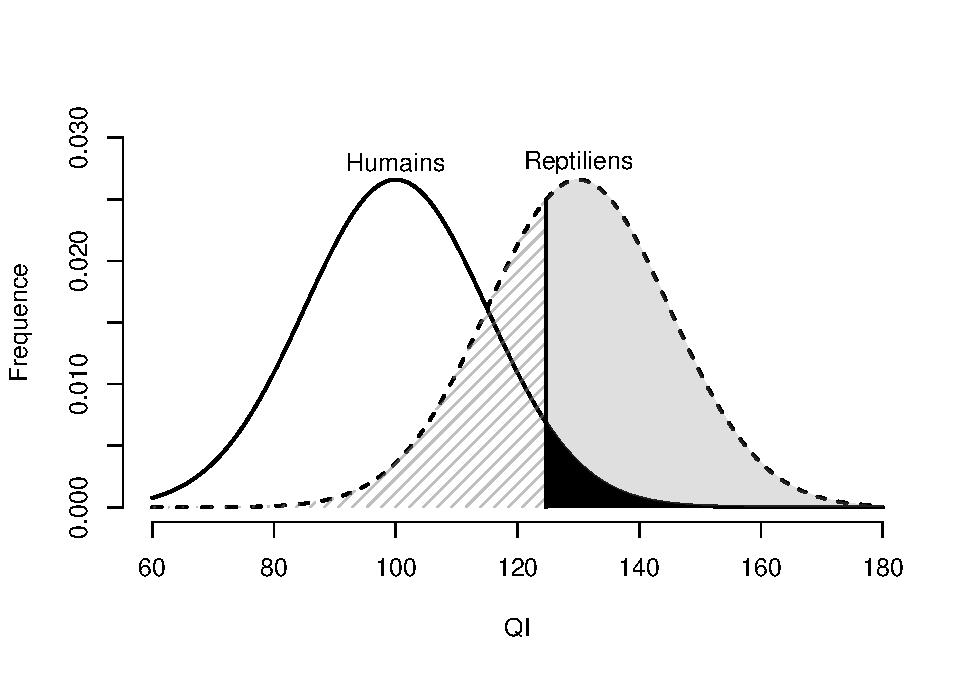
\includegraphics[width=0.9\linewidth,height=0.9\textheight]{03-Inferences_files/figure-latex/rh-1} 

}

\caption{Distribution du QI des humains et des reptiliens}\label{fig:rh}
\end{figure}

L'erreur de type I (présentée auparavant) représente la probabilité d'émettre un faux positif, souvent représentée par \(\alpha\) (alpha). Elle correspond à la probabilité de rejeter l'hypothèse lorsqu'elle est vraie. Dans la Figure \ref{fig:rh}, il s'agit de la zone noire. Elle corresond à conclure qu'un vrai humain est un reptilien (ce qu'il n'est pas). Ce taux est fixé à l'avance par l'expérimentateur, ici, 5\%. C'est le risque qu'il est prêt à prendre. Ainsi, 95\% des humains seront correctement identifiés comme humains.

\begin{Shaded}
\begin{Highlighting}[]
\CommentTok{\# Erreur de type I (fixé à l\textquotesingle{}avance)}
\NormalTok{alpha }\OtherTok{\textless{}{-}}\NormalTok{ .}\DecValTok{05} 

\CommentTok{\# Valeur critique à laquelle l\textquotesingle{}expérimentateur rejette H0}
\NormalTok{v.crit }\OtherTok{\textless{}{-}} \FunctionTok{qnorm}\NormalTok{(}\DecValTok{1} \SpecialCharTok{{-}}\NormalTok{ alpha, }\AttributeTok{mean =}\NormalTok{ mu.h, }\AttributeTok{sd =}\NormalTok{ sd.h)}
\NormalTok{v.crit}
\CommentTok{\#\textgreater{} [1] 125}

\CommentTok{\# Erreur de type II}
\NormalTok{beta }\OtherTok{\textless{}{-}} \FunctionTok{pnorm}\NormalTok{(v.crit, }\AttributeTok{mean =}\NormalTok{ mu.r, }\AttributeTok{sd =}\NormalTok{ sd.r)}
\NormalTok{beta}
\CommentTok{\#\textgreater{} [1] 0.361}

\CommentTok{\# Puissance statistique}
\NormalTok{puissance }\OtherTok{\textless{}{-}} \DecValTok{1} \SpecialCharTok{{-}}\NormalTok{ beta}
\NormalTok{puissance }
\CommentTok{\#\textgreater{} [1] 0.639}
\end{Highlighting}
\end{Shaded}

La zone hachurée de la Figure \ref{fig:rh} correspond à l'\textbf{erreur de type II}, souvent représentée par \(\beta\) (beta), soit la probabilité de \emph{ne pas rejeter} l'hypothèse nulle. Autrement dit, c'est la probabilité de ne pas trouver l'effet lorsque celui-ci est vrai. Pour cet exemple, il s'agit d'un reptilien assez sournois (avec un QI suffisamment faible pour sa population) qu'il passe inaperçu auprès des humains, ou, en d'autres termes, de conclure qu'un vrai reptilien est un humain (ce qu'il n'est pas). Cette probabilité est estimée à 36.124\%, donc 36.124\% des reptiliens passeront inaperçus.

La \textbf{puissance}, la zone grise de la Figure \ref{fig:rh}, correspond à la probabilité de rejeter correctement l'hypothèse nulle. Il s'agit de rejeter l'hypothèse nulle lorsqu'elle est fausse. Cela signifie d'identifier un vrai reptilien correctement. C'est exactement ce que le groupe de chercheur désire réaliser. Elle est estimée à 63.876\% en ne prenant qu'une mesure de QI. La puissance est l'une des statistiques qui intéressent le plus l'expérimentateur \emph{avant} de réaliser son étude, car elle donne une approximation sur la probabilité de trouver un résultat significatif. Par contre, les expérimentateurs ne connaissent que rarement les paramètres de la vraie distribution de l'effet qu'il désire trouver. En langage statistique, il s'agit un paramètre de non-centralité (ou de décentralisation) ou \texttt{ncp} en syntaxe \textbf{R}. L'expérimentateur recourt alors à d'habiles approximations éclairées basées sur leurs connaissances du phénomène et en regard des études déjà publiées sur le sujet (ou un sujet similaire), s'il y en a. Ces estimations souffrent tout de même d'être des variables aléatoires (elles respectent elles aussi une distribution d'échantillonnage), et non les paramètres recherchés.

Avant de procéder davantage, une dernière notion est importante à présenter : la direction du test. Dans tous les exemples précédents, l'hypothèse nulle était rejetée si une valeur plus rare était obtenue. Il s'agit d'un test d'hypothèse \textbf{unilatérale} (d'un seul côté). Cela facilite grandement la présentation de certains concepts et calculs. Un test peut être unilatérale inférieure, trouver un résultat plus faible qu'une valeur critique; ou unilatérale supérieure, trouver un résultat plus élevé qu'une valeur critique; ou encore \textbf{bilatérale}, soit trouver un résultat moins élevée ou plus élevée que des valeurs critiques.

Dans le cas d'un test bilatéral, l'erreur de type I est divisée par 2, \(\alpha/2\) pour couvrir l'espace des deux côtés de la distribution. L'espace total est identique même s'il est divisé sur les deux extrêmes. Cela implique des valeurs critiques plus élevées que si le test n'était que d'un côté et par conséquent une puissance statistique un peu plus faible, car l'effet est directionnel. La probabilité de rejeter l'hypothèse dans une direction a été diminuée pour tenir compte de l'autre côté. La Figure \ref{fig:tt} montre un exemple de chacun de ces types de tests pour \(\alpha = .05\).

\begin{figure}

{\centering 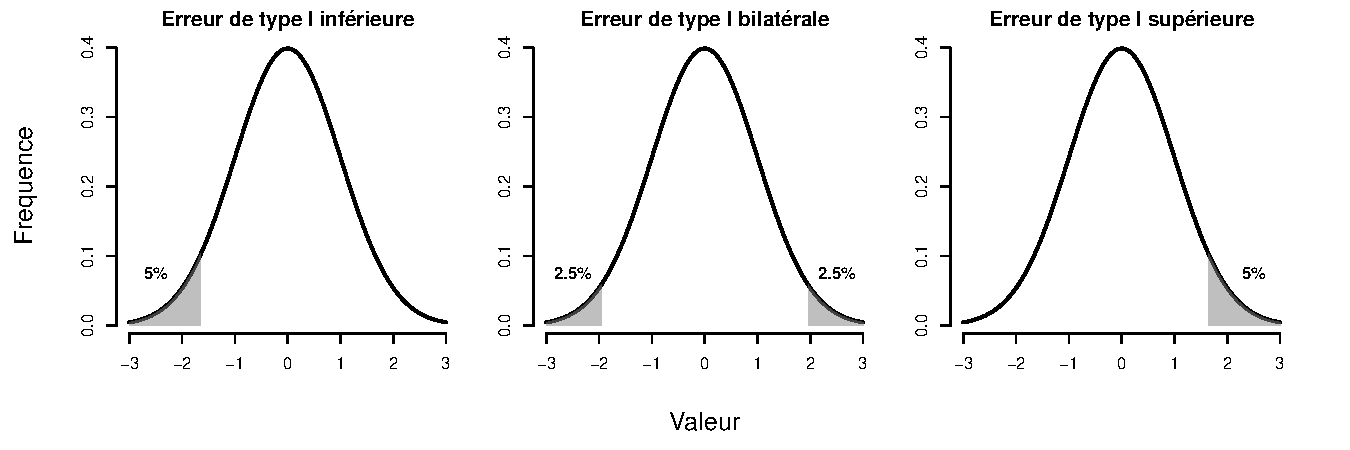
\includegraphics{03-Inferences_files/figure-latex/tt-1} 

}

\caption{Illustration de l'erreur de type I}\label{fig:tt}
\end{figure}

Le choix entre unilatérale inférieure, supérieure ou bilatérale repose essentiellement sur la question de recherche de l'expérimentateur. Qu'attend-il ou que veut-il savoir du résultat? L'expérimentateur recourt généralement au test bilatéral afin d'identifier des résultats allant pour son hypothèse ou à l'opposé de son hypothèse. Cela permet notamment d'identifier des devis qui pourraient nuire aux participants. Par exemple, si un expérimentateur développe une intervention pour réduire la consommation de drogues chez les adolescents et n'est concerné que par la probabilité que l'intervention soit efficace, il pourrait manquer l'effet délétère d'une telle intervention, soit que l'intervention augmente la consommation de drogue. Il est certain que l'expérimentateur souhaite être rapidement mis au courant si ces résultats se dessinent.

\hypertarget{la-distribution-t}{%
\section{\texorpdfstring{La distribution-\(t\)}{La distribution-t}}\label{la-distribution-t}}

Dans la plupart des cas, l'expérimentateur ne connaît pas la variance de la population. Il recourt alors à la meilleure estimation qui lui est disponible, celle obtenue auprès de l'échantillon. De recourir à une estimation au lieu de la vraie valeur cause un réel problème: l'estimation est une variable aléatoire respectant une distribution d'échantillonnage. La distribution des variances montre une légère asymétrie positive plus flagrante pour les petites tailles d'échantillon, car les variances sont distribuées en distribution-\(\chi^2\).

\begin{figure}
\centering
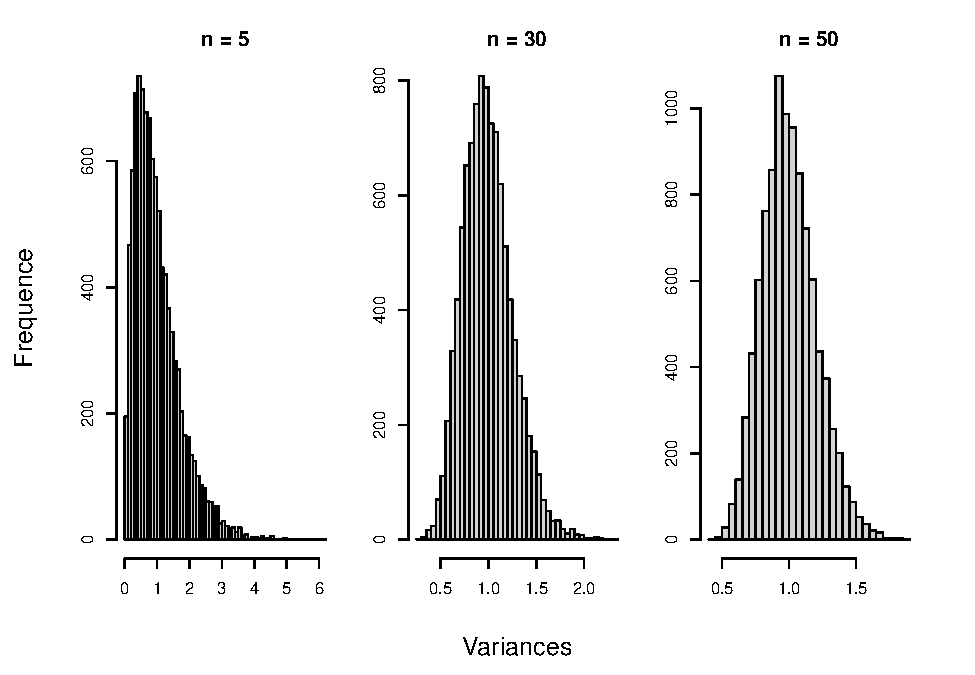
\includegraphics{03-Inferences_files/figure-latex/illvar-1.pdf}
\caption{\label{fig:illvar}Distribution de la variance en fonction de la taille d'échantillon}
\end{figure}

Une petite simulation faite à partir d'une distribution normale standardisée par rapport à trois tailles d'échantillon et dont la variance est estimée \ensuremath{10^{4}} fois est présentée dans la Figure \ref{fig:illvar}. Elle montre que l'estimation n'est pas biaisée (elles sont toutes les trois centrées à 1), mais relève l'asymétrie en question pour les petites tailles d'échantillon qui tend à décroître à mesure que \(n\) augmente. Autrement dit, une estimation unique (pris d'un échantillon) est plus susceptible d'être sous-estimée. Ne pas tenir compte de cet aspect augmente indûment les valeurs obtenues (à cause du dénominateur plus petit). Ainsi, il est inadéquat d'utiliser une distribution normale lorsque la variance est inconnue. Il faudra plutôt opter pour la \textbf{distribution-\(t\)} qui, elle, tient compte de la variabilité de l'estimation de la variance.

La distribution-\(t\) est symétrique, comme la distribution normale, mais a des queues plus larges pour tenir compte de la surestimation des valeurs dû à la sous-estimation de la variance. La distribution-\(t\) tend vers une distribution normale lorsque \(n\) augmente, ce qui est illustré à la Figure \ref{fig:tnorm}. La ligne pleine noire montre la distribution pour 5 unités, les deux autres lignes, traits et pointillés, pour 30 et 1000 unités respectivement. Il est difficile de distinguer ces deux dernières.

\begin{figure}

{\centering 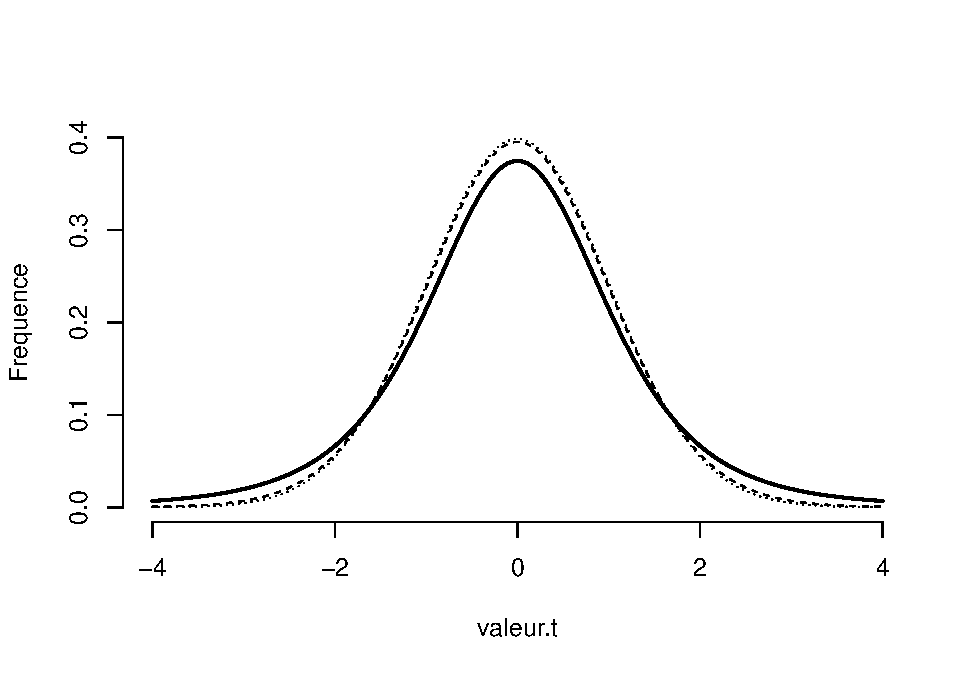
\includegraphics[width=0.9\linewidth,height=0.9\textheight]{03-Inferences_files/figure-latex/tnorm-1} 

}

\caption{Comparaison d'une distribution normale à deux distributions-$t$}\label{fig:tnorm}
\end{figure}

En ayant recours à des échantillons et une estimation de la variance (la variance est inconnue de l'expérimentateur, ce qui est généralement le cas), il faudra procéder avec la distribution-\(t\). La procédure est la même que celle utilisée avec les scores-\(z\) précédemment, la différence étant que la distribution-\(t\) est utilisée au lieu de la distribution normale, car l'écart type est estimé.

\hypertarget{le-test-t-uxe0-uxe9chantillon-unique}{%
\section{\texorpdfstring{Le test-\(t\) à échantillon unique}{Le test-t à échantillon unique}}\label{le-test-t-uxe0-uxe9chantillon-unique}}

Le test-\(t\) à échantillon unique permet de tester la moyenne d'échantillon par rapport à une valeur arbitraire \(\mu_0\) (généralement \(\mu_0 = 0\)) qui joue le rôle d'hypothèse nulle.

\[ t_{n-1} = \frac{\bar{x}-\mu_0}{(s/\sqrt{n})} \]

La distribution-\(t\) a un degré de liberté (l'indice de \(t\) dans l'équation) qui lui est associé et qui est fixé à \(dl = n - 1\), la taille d'échantillon moins 1. Un degré est perdu à cause de l'estimation de l'écart type de l'échantillon. Qu'en est-il de la probabilité d'obtenir cette moyenne? En recourant à la distribution intégrée de \textbf{R}, \texttt{pt()} il est possible d'obtenir la probabilité d'une valeur-\(t\) par rapport à l'hypothèse nulle. La fonction nécessite une valeur-\(t\) et le degré de liberté associé, p.~ex., \texttt{pt(t\ =\ ,\ df\ =\ n\ -\ 1)}. La valeur produite donne la probabilité d'obtenir un score plus petit jusqu'à la valeur-\(t\). Une astuce permet de calculer aisément la probabilité lorsque la distribution d'échantillonnage est symétrique. Utiliser une valeur absolue permet de considérer les deux côtés de la distribution simultanément. Les valeurs-\(t\) négatives sont alors positives. Comme un côté est supprimé, l'espace positif est doublé, le code pour tenir compte de cet astuce est : \texttt{(1\ -\ pt(abs(t),\ df\ =\ n\ -\ 1))\ *\ 2} où \texttt{t} est la valeur-\(t\) obtenue.

\begin{Shaded}
\begin{Highlighting}[]
\NormalTok{testt }\OtherTok{\textless{}{-}} \ControlFlowTok{function}\NormalTok{(x, }\AttributeTok{mu =} \DecValTok{0}\NormalTok{)\{}
  \CommentTok{\# x est une variable continue}
  \CommentTok{\# mu est une moyenne à tester comme hypothèse nulle(H0)}
\NormalTok{  xbar }\OtherTok{\textless{}{-}} \FunctionTok{mean}\NormalTok{(x)}
\NormalTok{  sdx }\OtherTok{\textless{}{-}} \FunctionTok{sd}\NormalTok{(x)}
\NormalTok{  n }\OtherTok{\textless{}{-}} \FunctionTok{length}\NormalTok{(x)}
\NormalTok{  vt }\OtherTok{\textless{}{-}}\NormalTok{ (xbar }\SpecialCharTok{{-}}\NormalTok{ mu) }\SpecialCharTok{/}\NormalTok{ (sdx }\SpecialCharTok{/} \FunctionTok{sqrt}\NormalTok{(n))}
\NormalTok{  dl }\OtherTok{\textless{}{-}}\NormalTok{ n }\SpecialCharTok{{-}} \DecValTok{1}
\NormalTok{  vp }\OtherTok{\textless{}{-}}\NormalTok{ (}\DecValTok{1} \SpecialCharTok{{-}} \FunctionTok{pt}\NormalTok{(}\FunctionTok{abs}\NormalTok{(vt), }\AttributeTok{df =}\NormalTok{ dl)) }\SpecialCharTok{*} \DecValTok{2} 
\NormalTok{  statistique }\OtherTok{\textless{}{-}} \FunctionTok{list}\NormalTok{(}\AttributeTok{valeur.t =}\NormalTok{ vt, }
                      \AttributeTok{dl =}\NormalTok{ dl, }
                      \AttributeTok{valeur.p =}\NormalTok{ vp)}
  \FunctionTok{return}\NormalTok{(statistique)}
\NormalTok{\}}
\end{Highlighting}
\end{Shaded}

Une fois la fonction créée, il est possible de la tester en la comparant avec la fonction \textbf{R} de base \texttt{test.t()}. Le code suivant crée un échantillon de 30 unités avec une moyenne de 1 et un écart type de 1.

\begin{Shaded}
\begin{Highlighting}[]
\CommentTok{\# Un exemple de jeu de données}
\FunctionTok{set.seed}\NormalTok{(}\DecValTok{20}\NormalTok{)}
\NormalTok{x }\OtherTok{=} \FunctionTok{rnorm}\NormalTok{(}\AttributeTok{n =} \DecValTok{30}\NormalTok{, }\AttributeTok{mean =} \DecValTok{1}\NormalTok{, }\AttributeTok{sd =} \DecValTok{1}\NormalTok{)}
\CommentTok{\# Vérification de la fonction maison}
\FunctionTok{testt}\NormalTok{(x)}
\CommentTok{\#\textgreater{} $valeur.t}
\CommentTok{\#\textgreater{} [1] 3.69}
\CommentTok{\#\textgreater{} }
\CommentTok{\#\textgreater{} $dl}
\CommentTok{\#\textgreater{} [1] 29}
\CommentTok{\#\textgreater{} }
\CommentTok{\#\textgreater{} $valeur.p}
\CommentTok{\#\textgreater{} [1] 0.000919}
\CommentTok{\# Comparer avec la fonction R}
\FunctionTok{t.test}\NormalTok{(x)}
\CommentTok{\#\textgreater{} }
\CommentTok{\#\textgreater{}  One Sample t{-}test}
\CommentTok{\#\textgreater{} }
\CommentTok{\#\textgreater{} data:  x}
\CommentTok{\#\textgreater{} t = 4, df = 29, p{-}value = 9e{-}04}
\CommentTok{\#\textgreater{} alternative hypothesis: true mean is not equal to 0}
\CommentTok{\#\textgreater{} 95 percent confidence interval:}
\CommentTok{\#\textgreater{}  0.31 1.08}
\CommentTok{\#\textgreater{} sample estimates:}
\CommentTok{\#\textgreater{} mean of x }
\CommentTok{\#\textgreater{}     0.696}
\end{Highlighting}
\end{Shaded}

\begin{figure}

{\centering 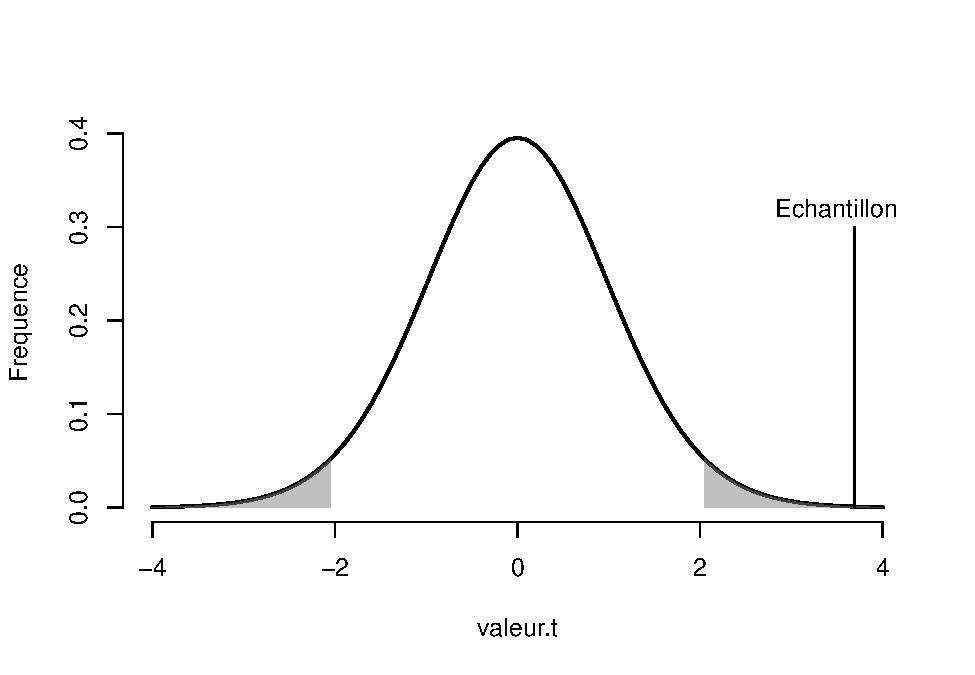
\includegraphics[width=0.75\linewidth,height=0.75\textheight]{03-Inferences_files/figure-latex/sss-1} 

}

\caption{Valeur-$t$ de l'échantillon sur la distribution-$t$}\label{fig:sss}
\end{figure}

Qu'est-ce que ces résultats signifient? La Figure \ref{fig:sss} montre la distribution d'échantillonnage de l'hypothèse nulle, c'est-à-dire l'hypothèse selon laquelle la moyenne de la population est égale à 0. Les zones grises montrent les zones de rejet. Si une valeur-\(t\) se retrouve dans ces zones, elle est jugée comme \emph{trop rare}, il faut alors rejeter l'hypothèse nulle. C'est ce qui s'est produit ici. Rien de surprenant, l'échantillon est tiré d'une distribution normale avec une moyenne de 1 et un écart type de 1.

\hypertarget{critiques-des-tests-dhypothuxe8ses}{%
\section{Critiques des tests d'hypothèses}\label{critiques-des-tests-dhypothuxe8ses}}

\emph{(Cette section est en construction.)}

Le présent ouvrage ne couvre que l'aspect traditionnel ou classique des tests d'hypothèse. Cette approche est remise en question depuis 1950 jusqu'à aujourd'hui. D'excellents ouvrages couvrent les failles et solutions des tests d'hypothèses classiques de façon plus approfondie qu'il ne l'est fait ici.

\begin{itemize}
\tightlist
\item
  L'hypothèse nulle n'est jamais susceptible d'être vraie.
\item
  La conclusion statistique n'est pas celle désirée par l'expérimentateur.
\item
  La significativité statistique n'implique pas la significativité pratique.
\item
  Les expérimentateurs interprètent incorrectement la valeur-\(p\).
\item
  Une valeur-\(p\) faible n'est pas garantie de la reproductibilité.
\item
  La dichotomisation de la preuve \(p<=\alpha\).
\item
  Une saine utilisation de la valeur-\(p\) n'accomplit pas grand-chose.
\item
  L'obsession de la valeur-\(p\) cause plus de problèmes qu'elle n'en résout : \(p\)-hacking, triturage de données, abus de variables, comparaison multiple, biais pour les hypothèses originales et surprenantes.
\end{itemize}

\hypertarget{analyser}{%
\chapter{Analyser}\label{analyser}}

En continuation de l'introduction des théories des tests d'hypothèses (voir \protect\hyperlink{infuxe9rer}{Inférer}) et l'aperçu donnée par \protect\hyperlink{le-test-t-uxe0-uxe9chantillon-unique}{le test-\(t\) à échantillon unique}, cette section poursuit la présentation en introduisant des analyses statistiques de bases comme les différences de moyennes, l'association linéaire et les tests pour données nominales. Les tests-\(t\) indépendant et dépendant, l'analyse de variables, la covariance, la corrélation ainsi que le test du \(\chi2\) pour table de contingence sont présentées.

\hypertarget{les-diffuxe9rences-de-moyennes}{%
\section{Les différences de moyennes}\label{les-diffuxe9rences-de-moyennes}}

\hypertarget{test-t-induxe9pendant}{%
\subsection{\texorpdfstring{Test-\emph{t} indépendant}{Test-t indépendant}}\label{test-t-induxe9pendant}}

En général, l'expérimentateur ne s'intéresse pas à comparer une moyenne à une valeur arbitraire, comme c'était le cas avec \protect\hyperlink{le-test-t-uxe0-uxe9chantillon-unique}{le test-\(t\) à échantillon unique}. Cela peut lui être assez trivial. Il s'intéresse plutôt à comparer une moyenne à une autre moyenne, soit une différence entre deux groupes indépendants, par exemple, quel est la différence entre un groupe traitement et un groupe contrôle?

En se basant sur le test \(t\) à échantillon unique, la valeur-\(t\) pour deux moyennes se calcule selon l'équation \eqref{eq:test2}

\begin{equation}
t_{n-2} = \frac{\bar{x_1}-\bar{x_2}}{\sqrt{\frac{s^2_{1}}{n_1}+\frac{s^2_{2}}{n_2}}}
\label{eq:test2}
\end{equation}

où l'indice de la valeur-\(t\) est le nombre de degrés de liberté \(n-2\). Comme deux variances sont estimées, deux degrés de libertés sont imputés, ce qui octroi \(n-2\) degrés. En plus de considéré \(\bar{x_2}\) la valeur \emph{arbitaire} de comparaison (l'ordre de \(\bar{x_2}\) et \(\bar{x^1}\) est arbitraire), les deux écart types sont également considérés au dénominateur.

Une fois le calcul réalisé, la logique du test d'hypothèse est la même, à l'exception de l'hypothèse nulle qui correspond maintenant à l'absence de différence entre les deux moyennes.

Voici un exemple de programmation du test-\(t\) pour deux groupes indépendants.

\begin{Shaded}
\begin{Highlighting}[]
\NormalTok{testt.ind }\OtherTok{\textless{}{-}} \ControlFlowTok{function}\NormalTok{(x1, x2)\{}
  \CommentTok{\# x1 est une variable continue associée au groupe 1}
  \CommentTok{\# x2 est une variable continue associée au groupe 2}
  
  \CommentTok{\# Calcul des moyennes}
\NormalTok{  x1bar }\OtherTok{\textless{}{-}} \FunctionTok{mean}\NormalTok{(x1) ; x2bar }\OtherTok{\textless{}{-}} \FunctionTok{mean}\NormalTok{(x2)}
  
  \CommentTok{\# Calcul des variances}
\NormalTok{  x1var }\OtherTok{\textless{}{-}} \FunctionTok{var}\NormalTok{(x1) ; x2var }\OtherTok{\textless{}{-}} \FunctionTok{var}\NormalTok{(x2)}
  
  \CommentTok{\# Calcul des tailles d\textquotesingle{}échantillon}
\NormalTok{  nx1 }\OtherTok{\textless{}{-}} \FunctionTok{length}\NormalTok{(x1) ; nx2 }\OtherTok{\textless{}{-}} \FunctionTok{length}\NormalTok{(x2)}
  
  \CommentTok{\# Valeur{-}t, degrés de liberté et valeur{-}p}
\NormalTok{  vt }\OtherTok{\textless{}{-}}\NormalTok{ (x1bar }\SpecialCharTok{{-}}\NormalTok{ x2bar) }\SpecialCharTok{/} \FunctionTok{sqrt}\NormalTok{(x1var }\SpecialCharTok{/}\NormalTok{ nx1 }\SpecialCharTok{+}\NormalTok{ x2var }\SpecialCharTok{/}\NormalTok{ nx2)}
\NormalTok{  dl }\OtherTok{\textless{}{-}}\NormalTok{ nx1 }\SpecialCharTok{+}\NormalTok{ nx2 }\SpecialCharTok{{-}} \DecValTok{2}
\NormalTok{  vp }\OtherTok{\textless{}{-}}\NormalTok{ (}\DecValTok{1} \SpecialCharTok{{-}} \FunctionTok{pt}\NormalTok{(}\FunctionTok{abs}\NormalTok{(vt), }\AttributeTok{df =}\NormalTok{ dl)) }\SpecialCharTok{*} \DecValTok{2} 
\NormalTok{  statistique }\OtherTok{\textless{}{-}} \FunctionTok{list}\NormalTok{(}\AttributeTok{valeur.t =}\NormalTok{ vt, }\AttributeTok{dl =}\NormalTok{ dl, }\AttributeTok{valeur.p =}\NormalTok{ vp)}
  \FunctionTok{return}\NormalTok{(statistique)}
\NormalTok{\}}
\end{Highlighting}
\end{Shaded}

Pour générer un exemple de données, le code ci-après crée un échantillon de 15 unités réparties en deux groupes, le premier groupe (\texttt{gr0}) est tiré d'une distribution normale ayant une moyenne de 1 et un écart type de 1, le deuxième groupe (\texttt{gr1}), une moyenne de 0 et un écart type de 1. La syntaxe illustre la création de deux variables pour créer les deux groupes. Il est aussi possible d'envisager la création sur en termes d'équation linéaire,

\[y = \mu_0 + \mu_1x_1 + \epsilon\]
où \(y\) est le score observé des unités et les autres variables construisent ce score, \(\mu_0\) correspond à la moyenne du groupe référent de population (le groupe ``contrôle'' en quelque sorte.), \(\mu_1\) réfère à la différence de moyenne entre les deux groupes identifiés par \(x_1\) qui réfère à l'assignation au groupe, soit 0 pour le groupe ``contrôle'' et 1 pour le groupe ``différent''. Pour ce même exemple, \(\mu_1 = -1\). Par le produit \(\mu_1x_1\), le groupe ``contrôle'' associé à la valeur 0 n'a pas de modification de la moyenne, \(-1*0=0\) alors le groupe ``différent'' associé à la valeur 1, \(-1*1=-1\). Enfin, \(\epsilon\) correspond à la variabilité entre les unités. Cette façon de programmer la création des variables illustre bien l'association linéaire qui existe même dans les différences de moyennes et sera très utile pour des modèles plus compliqués.

\begin{Shaded}
\begin{Highlighting}[]
\CommentTok{\# Un exemple de jeu de données programmé de deux façons}
\CommentTok{\# Méthode 1}
\FunctionTok{set.seed}\NormalTok{(}\DecValTok{2021}\NormalTok{)}
\NormalTok{gr0 }\OtherTok{\textless{}{-}} \FunctionTok{rnorm}\NormalTok{(}\AttributeTok{n =} \DecValTok{15}\NormalTok{, }\AttributeTok{mean =} \DecValTok{1}\NormalTok{, }\AttributeTok{sd =} \DecValTok{1}\NormalTok{)}
\NormalTok{gr1 }\OtherTok{\textless{}{-}} \FunctionTok{rnorm}\NormalTok{(}\AttributeTok{n =} \DecValTok{15}\NormalTok{, }\AttributeTok{mean =} \DecValTok{0}\NormalTok{, }\AttributeTok{sd =} \DecValTok{1}\NormalTok{)}

\CommentTok{\# Méthode 2}
\FunctionTok{set.seed}\NormalTok{(}\DecValTok{2021}\NormalTok{)}
\NormalTok{x1 }\OtherTok{\textless{}{-}} \FunctionTok{c}\NormalTok{(}\FunctionTok{rep}\NormalTok{(}\DecValTok{0}\NormalTok{, }\DecValTok{15}\NormalTok{), }\FunctionTok{rep}\NormalTok{(}\DecValTok{1}\NormalTok{, }\DecValTok{15}\NormalTok{)) }\CommentTok{\# Appartenance au groupe (0 et 1)}
\NormalTok{e }\OtherTok{\textless{}{-}} \FunctionTok{rnorm}\NormalTok{(}\AttributeTok{n =} \DecValTok{30}\NormalTok{, }\AttributeTok{mean =} \DecValTok{0}\NormalTok{, }\AttributeTok{sd =} \DecValTok{1}\NormalTok{) }\CommentTok{\# Erreur interindividuel}
\NormalTok{mu1 }\OtherTok{\textless{}{-}} \SpecialCharTok{{-}}\DecValTok{1} \CommentTok{\# le deuxième groupe a une différence de moyenne de {-}1}
\NormalTok{mu0 }\OtherTok{\textless{}{-}} \DecValTok{1} \CommentTok{\# moyenne du groupe référent}
\NormalTok{y }\OtherTok{\textless{}{-}}\NormalTok{ mu0 }\SpecialCharTok{+}\NormalTok{ mu1 }\SpecialCharTok{*}\NormalTok{ x1 }\SpecialCharTok{+}\NormalTok{ e}
\CommentTok{\# Présenter quelques participants; retirer les crochets pour voir tous}
\NormalTok{(}\FunctionTok{cbind}\NormalTok{(}\AttributeTok{method1 =} \FunctionTok{c}\NormalTok{(gr0, gr1), }\AttributeTok{method2 =}\NormalTok{ y))[}\DecValTok{10}\SpecialCharTok{:}\DecValTok{20}\NormalTok{,]}
\CommentTok{\#\textgreater{}       method1 method2}
\CommentTok{\#\textgreater{}  [1,]  2.7300  2.7300}
\CommentTok{\#\textgreater{}  [2,] {-}0.0822 {-}0.0822}
\CommentTok{\#\textgreater{}  [3,]  0.7272  0.7272}
\CommentTok{\#\textgreater{}  [4,]  1.1820  1.1820}
\CommentTok{\#\textgreater{}  [5,]  2.5085  2.5085}
\CommentTok{\#\textgreater{}  [6,]  2.6045  2.6045}
\CommentTok{\#\textgreater{}  [7,] {-}1.8415 {-}1.8415}
\CommentTok{\#\textgreater{}  [8,]  1.6233  1.6233}
\CommentTok{\#\textgreater{}  [9,]  0.1314  0.1314}
\CommentTok{\#\textgreater{} [10,]  1.4811  1.4811}
\CommentTok{\#\textgreater{} [11,]  1.5133  1.5133}
\end{Highlighting}
\end{Shaded}

Les données sont identiques.

Une fois la fonction créée, il est possible de la tester et de la comparer avec la fonction \textbf{R} de base \texttt{test.t()}.

\begin{Shaded}
\begin{Highlighting}[]
\CommentTok{\# Vérification de la fonction maison}
\FunctionTok{testt.ind}\NormalTok{(gr0, gr1)}
\CommentTok{\#\textgreater{} $valeur.t}
\CommentTok{\#\textgreater{} [1] 3.4}
\CommentTok{\#\textgreater{} }
\CommentTok{\#\textgreater{} $dl}
\CommentTok{\#\textgreater{} [1] 28}
\CommentTok{\#\textgreater{} }
\CommentTok{\#\textgreater{} $valeur.p}
\CommentTok{\#\textgreater{} [1] 0.00205}
\CommentTok{\# Comparer avec la fonction R}
\FunctionTok{t.test}\NormalTok{(gr0, gr1, }\AttributeTok{var.equal =} \ConstantTok{TRUE}\NormalTok{)}
\CommentTok{\#\textgreater{} }
\CommentTok{\#\textgreater{}  Two Sample t{-}test}
\CommentTok{\#\textgreater{} }
\CommentTok{\#\textgreater{} data:  gr0 and gr1}
\CommentTok{\#\textgreater{} t = 3, df = 28, p{-}value = 0.002}
\CommentTok{\#\textgreater{} alternative hypothesis: true difference in means is not equal to 0}
\CommentTok{\#\textgreater{} 95 percent confidence interval:}
\CommentTok{\#\textgreater{}  0.54 2.18}
\CommentTok{\#\textgreater{} sample estimates:}
\CommentTok{\#\textgreater{} mean of x mean of y }
\CommentTok{\#\textgreater{}     1.332    {-}0.029}
\end{Highlighting}
\end{Shaded}

Les équations et codes précédents ne sont adéquats que si les variances sont égales entre les deux groupes. Cette notion est quelque peu trahie par la spécification dans la fonction \textbf{R} de l'argument \texttt{var.equal\ =\ TRUE} qui par défaut est \texttt{FALSE}. Pour un test-\(t\) indépendant suivant les règles de l'art, il faut appliquer une correction (approximation de Welsh) aux degrés de liberté. Les degrés de liberté deviennent moins élégants, le code devient ainsi.

\[
dl=\frac{\left(\frac{s^2_1}{n_1}+\frac{s^2_2}{n_2}\right)^2}{\frac{\left(\frac{s^2_1}{n_1}\right)^2}{n_1-1}+\frac{\left(\frac{s^2_2}{n_2}\right)^2}{n_2-1}}
\]
En apportant cette correction au code initial.

\begin{Shaded}
\begin{Highlighting}[]
\NormalTok{testt.ind2 }\OtherTok{\textless{}{-}}\ControlFlowTok{function}\NormalTok{(x1, x2)\{}
  \CommentTok{\# x1 est une variable continue associée au groupe 1}
  \CommentTok{\# x2 est une variable continue associée au groupe 2}
\NormalTok{  x1bar }\OtherTok{\textless{}{-}} \FunctionTok{mean}\NormalTok{(x1) ; x2bar }\OtherTok{\textless{}{-}} \FunctionTok{mean}\NormalTok{(x2)}
\NormalTok{  x1var }\OtherTok{\textless{}{-}} \FunctionTok{var}\NormalTok{(x1) ; x2var }\OtherTok{\textless{}{-}} \FunctionTok{var}\NormalTok{(x2)}
\NormalTok{  nx1 }\OtherTok{\textless{}{-}} \FunctionTok{length}\NormalTok{(x1) ; nx2 }\OtherTok{\textless{}{-}} \FunctionTok{length}\NormalTok{(x2)}
  
  \CommentTok{\# erreur type }
\NormalTok{  et }\OtherTok{\textless{}{-}} \FunctionTok{sqrt}\NormalTok{(x1var }\SpecialCharTok{/}\NormalTok{ nx1 }\SpecialCharTok{+}\NormalTok{ x2var }\SpecialCharTok{/}\NormalTok{ nx2)}
  \CommentTok{\# valeur t}
\NormalTok{  vt }\OtherTok{\textless{}{-}}\NormalTok{ (x1bar }\SpecialCharTok{{-}}\NormalTok{ x2bar) }\SpecialCharTok{/}\NormalTok{ et}
  \CommentTok{\# correction des degrés de liberté}
\NormalTok{  dl }\OtherTok{\textless{}{-}}\NormalTok{ et}\SpecialCharTok{\^{}}\DecValTok{4} \SpecialCharTok{/} 
\NormalTok{    ((x1var}\SpecialCharTok{\^{}}\DecValTok{2} \SpecialCharTok{/}\NormalTok{ (nx1}\SpecialCharTok{\^{}}\DecValTok{2} \SpecialCharTok{*}\NormalTok{ (nx1 }\SpecialCharTok{{-}} \DecValTok{1}\NormalTok{))) }\SpecialCharTok{+}\NormalTok{ (x2var}\SpecialCharTok{\^{}}\DecValTok{2} \SpecialCharTok{/}\NormalTok{ (nx2}\SpecialCharTok{\^{}}\DecValTok{2} \SpecialCharTok{*}\NormalTok{ (nx2 }\SpecialCharTok{{-}} \DecValTok{1}\NormalTok{))))}
  \CommentTok{\# valeur{-}p}
\NormalTok{  vp }\OtherTok{\textless{}{-}}\NormalTok{ (}\DecValTok{1} \SpecialCharTok{{-}} \FunctionTok{pt}\NormalTok{(}\FunctionTok{abs}\NormalTok{(vt), }\AttributeTok{df =}\NormalTok{ dl)) }\SpecialCharTok{*} \DecValTok{2} 
\NormalTok{  statistique }\OtherTok{\textless{}{-}} \FunctionTok{list}\NormalTok{(}\AttributeTok{valeur.t =}\NormalTok{ vt, }\AttributeTok{dl =}\NormalTok{ dl, }\AttributeTok{valeur.p =}\NormalTok{ vp)}
  \FunctionTok{return}\NormalTok{(statistique)}
\NormalTok{\}}
\end{Highlighting}
\end{Shaded}

Le voici comparé la fonction \textbf{R} de base.

\begin{Shaded}
\begin{Highlighting}[]
\FunctionTok{t.test}\NormalTok{(gr0, gr1) }\CommentTok{\# Absence de l\textquotesingle{}argument var.equal = TRUE}
\CommentTok{\#\textgreater{} }
\CommentTok{\#\textgreater{}  Welch Two Sample t{-}test}
\CommentTok{\#\textgreater{} }
\CommentTok{\#\textgreater{} data:  gr0 and gr1}
\CommentTok{\#\textgreater{} t = 3, df = 27, p{-}value = 0.002}
\CommentTok{\#\textgreater{} alternative hypothesis: true difference in means is not equal to 0}
\CommentTok{\#\textgreater{} 95 percent confidence interval:}
\CommentTok{\#\textgreater{}  0.539 2.182}
\CommentTok{\#\textgreater{} sample estimates:}
\CommentTok{\#\textgreater{} mean of x mean of y }
\CommentTok{\#\textgreater{}     1.332    {-}0.029}
\FunctionTok{testt.ind2}\NormalTok{(gr0, gr1)}
\CommentTok{\#\textgreater{} $valeur.t}
\CommentTok{\#\textgreater{} [1] 3.4}
\CommentTok{\#\textgreater{} }
\CommentTok{\#\textgreater{} $dl}
\CommentTok{\#\textgreater{} [1] 26.9}
\CommentTok{\#\textgreater{} }
\CommentTok{\#\textgreater{} $valeur.p}
\CommentTok{\#\textgreater{} [1] 0.00213}
\end{Highlighting}
\end{Shaded}

Les sorties sont identiques.

\begin{figure}

{\centering 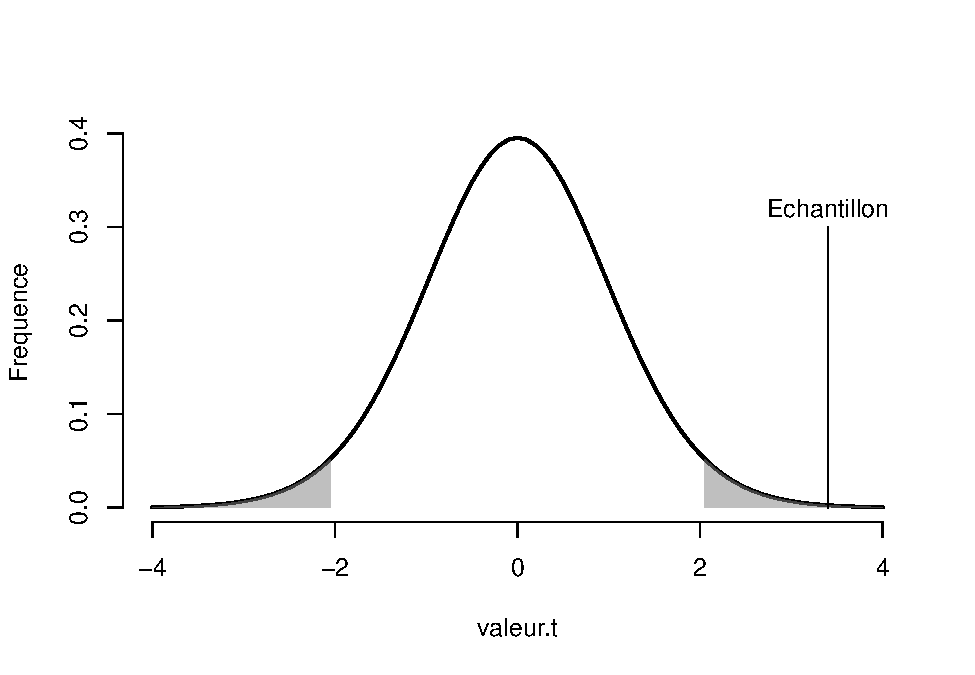
\includegraphics[width=0.75\linewidth,height=0.75\textheight]{04-Analyses_files/figure-latex/disttt-1} 

}

\caption{Valeur-$t$ de la différence de moyenne sur la distribution-$t$}\label{fig:disttt}
\end{figure}

La Figure \ref{fig:disttt} illustre où se situe la moyenne de l'échantillon par rapport à la distribution d'échantillonnage de l'hypothèse nulle. Comme la valeur se retrouve dans la zone de rejet ou, de façon équivalente, la valeur-\(p\) est plus petite que la valeur \(\alpha\) fixé (ici à 5\%), on rejette l'hypothèse nulle, il y a vraisemblablement une différence entre les groupes, ce qui était l'intention derrière la création des données.

\hypertarget{test-t-duxe9pendant}{%
\subsection{\texorpdfstring{Test-\emph{t} dépendant}{Test-t dépendant}}\label{test-t-duxe9pendant}}

Un dernier test-\(t\) a présenté est le test permettant de comparer deux de temps de mesure sur les mêmes participants. L'hypothèse désirée est de constater si \(\mu_1 = \mu_2\), soit la moyenne du temps 1 est égale à la moyenne du temps 2. Une habile manipulation mathématique permet de poser cette hypothèse en hypothèse nulle, \(\mu_1-\mu_2=0\). Il est intéressant de noter (ou de rappeler) que la différence entre deux variables est normalement distribuée si la variance est connue ou distribuée en \(t\) si la variance est inconnue.

Ce test est utile lorsqu'il faut tester si les participants se sont améliorés ou détériorés entre deux temps de mesure. Pour calculer la valeur-\(t\),

\[ t_{dl_1} = \frac{\bar{x_1}-\bar{x_2}}{\sigma_d/\sqrt{n}} \]

avec \(n-1\) degrés de liberté à cause de l'estimation de l'écart type. Les étapes subséquentes sont identiques au test-\(t\) à groupe unique.

\begin{Shaded}
\begin{Highlighting}[]
\NormalTok{testt.dep }\OtherTok{\textless{}{-}} \ControlFlowTok{function}\NormalTok{(temps1, temps2)\{}
  \CommentTok{\# temps est une variable continue mesurée }
  \CommentTok{\# à deux occasion auprès des mêmes participants}
\NormalTok{  difference }\OtherTok{\textless{}{-}}\NormalTok{ temps1 }\SpecialCharTok{{-}}\NormalTok{ temps2}
\NormalTok{  dbar }\OtherTok{\textless{}{-}} \FunctionTok{mean}\NormalTok{(difference)}
\NormalTok{  dvar }\OtherTok{\textless{}{-}} \FunctionTok{var}\NormalTok{(difference)}
\NormalTok{  n }\OtherTok{\textless{}{-}} \FunctionTok{length}\NormalTok{(difference)}
\NormalTok{  vt }\OtherTok{\textless{}{-}}\NormalTok{ (dbar) }\SpecialCharTok{/} \FunctionTok{sqrt}\NormalTok{(dvar }\SpecialCharTok{/}\NormalTok{ n)}
\NormalTok{  dl }\OtherTok{\textless{}{-}}\NormalTok{ n }\SpecialCharTok{{-}} \DecValTok{1}
\NormalTok{  vp }\OtherTok{\textless{}{-}}\NormalTok{ (}\DecValTok{1} \SpecialCharTok{{-}} \FunctionTok{pt}\NormalTok{(}\FunctionTok{abs}\NormalTok{(vt), }\AttributeTok{df =}\NormalTok{ dl)) }\SpecialCharTok{*} \DecValTok{2}
\NormalTok{  statistique }\OtherTok{\textless{}{-}} \FunctionTok{list}\NormalTok{(}\AttributeTok{valeur.t =}\NormalTok{ vt, }\AttributeTok{dl =}\NormalTok{ dl, }\AttributeTok{valeur.p =}\NormalTok{ vp)}
  \FunctionTok{return}\NormalTok{(statistique)}
\NormalTok{\}}
\end{Highlighting}
\end{Shaded}

Pour créer le jeu de données, les étapes sont similaires au test-\(t\) indépendant pour des temps de mesure indépendants (sans corrélation) où seules les populations des temps de mesure sont définis. Il est possible de spécifier une corrélation entre les deux de mesures. Cela sera introduit ultérieurement.

Dans ce jeu de données, 25 personnes sont mesurées à deux temps de reprises. Il n'y a pas de corrélation entre les temps de mesure. La variance des temps de mesure est de 1. La différence de moyenne est de 3.

\begin{Shaded}
\begin{Highlighting}[]
\CommentTok{\# Un exemple de jeu de données}
\FunctionTok{set.seed}\NormalTok{(}\DecValTok{148}\NormalTok{)}
\NormalTok{temps1 }\OtherTok{\textless{}{-}} \FunctionTok{rnorm}\NormalTok{(}\AttributeTok{n =} \DecValTok{25}\NormalTok{, }\AttributeTok{mean =} \DecValTok{0}\NormalTok{, }\AttributeTok{sd =} \DecValTok{2}\NormalTok{)}
\NormalTok{temps2 }\OtherTok{\textless{}{-}} \FunctionTok{rnorm}\NormalTok{(}\AttributeTok{n =} \DecValTok{25}\NormalTok{, }\AttributeTok{mean =} \DecValTok{3}\NormalTok{, }\AttributeTok{sd =} \DecValTok{2}\NormalTok{)}
\end{Highlighting}
\end{Shaded}

La fonction base de \textbf{R} est encore \texttt{t.test()}, mais il faudra spécifier l'argument \texttt{paired\ =\ TRUE} pour commander un test apparié (une autre appellation pour un test-\(t\) dépendant).

\begin{Shaded}
\begin{Highlighting}[]
\FunctionTok{t.test}\NormalTok{(temps1, temps2, }\AttributeTok{paired =} \ConstantTok{TRUE}\NormalTok{)}
\CommentTok{\#\textgreater{} }
\CommentTok{\#\textgreater{}  Paired t{-}test}
\CommentTok{\#\textgreater{} }
\CommentTok{\#\textgreater{} data:  temps1 and temps2}
\CommentTok{\#\textgreater{} t = {-}3, df = 24, p{-}value = 0.008}
\CommentTok{\#\textgreater{} alternative hypothesis: true difference in means is not equal to 0}
\CommentTok{\#\textgreater{} 95 percent confidence interval:}
\CommentTok{\#\textgreater{}  {-}3.268 {-}0.552}
\CommentTok{\#\textgreater{} sample estimates:}
\CommentTok{\#\textgreater{} mean of the differences }
\CommentTok{\#\textgreater{}                   {-}1.91}
\FunctionTok{testt.dep}\NormalTok{(temps1, temps2)}
\CommentTok{\#\textgreater{} $valeur.t}
\CommentTok{\#\textgreater{} [1] {-}2.9}
\CommentTok{\#\textgreater{} }
\CommentTok{\#\textgreater{} $dl}
\CommentTok{\#\textgreater{} [1] 24}
\CommentTok{\#\textgreater{} }
\CommentTok{\#\textgreater{} $valeur.p}
\CommentTok{\#\textgreater{} [1] 0.0078}
\end{Highlighting}
\end{Shaded}

Les sorties sont identiques.

\begin{figure}

{\centering 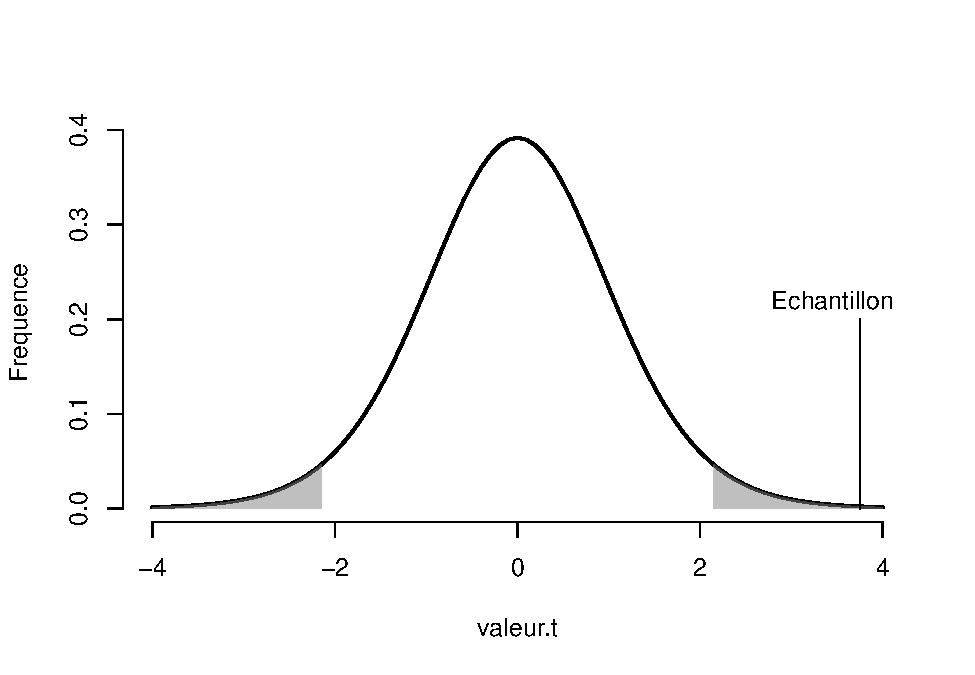
\includegraphics[width=0.75\linewidth,height=0.75\textheight]{04-Analyses_files/figure-latex/testtttt-1} 

}

\caption{Valeur-$t$ de moyenne de différences sur la distribution-$t$}\label{fig:testtttt}
\end{figure}

La Figure \ref{fig:testtttt} montre où se situe la différence de moyenne par rapport à la distribution d'échantillonnage de l'hypothèse nulle. Comme la valeur se retrouve dans la valeur-\(p\) est plus petite que la valeur \(\alpha\) fixée (ici à 5\%), on rejette l'hypothèse nulle, il y a vraisemblablement une différence entre les temps de mesure, ce qui était l'intention derrière la création des données.

\hypertarget{lanalyse-de-variance-uxe0-un-facteur}{%
\subsection{L'analyse de variance à un facteur}\label{lanalyse-de-variance-uxe0-un-facteur}}

L'analyse de variance, souvent appelée ANOVA (\emph{ANalysis Of VAriance}), permet de comparer une variable continue sur plusieurs groupes ou traitements. Il s'agit d'une extension du test-\(t\) indépendant qui compare une variable continue auprès de deux groupes. À plus de deux groupes, l'analyse de variance entre en jeu. \textbf{Attention!} Cette section se limite au cas où les groupes sont de tailles identiques (même nombre de participants par groupe, le symbole \(n_k\) pour référer à cette quantité) afin d'en simplifier la présentation.

\hypertarget{la-logique-de-lanalyse-de-variance}{%
\subsubsection{La logique de l'analyse de variance}\label{la-logique-de-lanalyse-de-variance}}

Comme il a été présenté dans la section sur le test-\(t\) indépendant, le modèle sous-jacent à l'analyse de variance à un facteur est une extension de ce modèle pour \(k\) groupes. Chaque groupe est associé à une différence de moyennes \(\mu_i\), pour \(i = 1,2, ...k\) par rapport à la moyenne groupe référent, \(\mu_0\). Les variables \(x_i\) définissent l'appartenance au groupe \(i\) par la valeur 1 et 0 pour les autres groupes (codage factice ou \emph{dummy coding}).

\[y = \mu_0 + \mu_1x_1 + \mu_2x_2+ ... +\mu_kx_k + \epsilon\]
L'hypothèse nulle est la suivante.
\[\sigma^2_1=\sigma^2_2=...=\sigma^2_k\]
L'analyse de variance est un test omnibus (global) qui ne teste pas où est la différence, mais bien \emph{s'il y a au moins une différence} entre les groupes. L'hypothèse nulle peut s'avérer fausse de plusieurs façons. Il peut y avoir une ou plusieurs inégalités pour rejeter l'hypothèse nulle.

La logique sous-jacente est basée sur l'idée selon laquelle les moyennes des groupes proviennent d'une même population. Elle compare les hypothèses suivantes : l'hypothèse nulle : les données (les moyennes) proviennent d'une même population; et l'hypothèse opposée : les données ne proviennent pas d'une même population.

Elle suggère ainsi deux types de variances (ou carré moyen, CM, dans ce contexte) : le CMI, carré moyen intergroupe, lorsque l'hypothèse nulle est vraie (la variabilité des moyennes); et le CMR, carré moyen résiduel, lorsque l'hypothèse nulle n'est ni vraie, ni fausse (la variabilité des données).

Pour calculer le CMI, la variance des moyennes des groupes est
\[s^2_{\bar{x}}=\sum_{i=1}^k\frac{(\bar{x_i}-\overline{\overline{x}})^2}{k-1}\]

où \(\overline{\overline{x}}\) est la grande moyenne (la moyenne de toutes les unités). Cette statistique se retrouve sur la plan des distributions d'échantillonnage (comment les moyennes se distribuent). Il faut ainsi multiplier cette valeur par \(n_k\), le nombre d'unités par groupes, pour obtenir une estimation de la variance de la population. Ainsi, \(\text{CMI} = s^2_{\bar{x}}n_k\).

Il y a plusieurs méthodes pour calculer le CMR, comme le CMR est envisagé comme la moyenne des variances de groupes, il est pratique d'en référer le calcul à sa définition.

\[
\text{CMR} = \bar{s^2} = \frac{1}{k}\sum_{i=k}^k\sigma_k^2 
\]
Lorsque l'hypothèse nulle est vraie, les variances des groupes sont traitées comme le résultat d'une étude sur une même population, comme si \(k\) petites études avaient été réalisées. L'estimation du CMI est de l'ordre d'une distribution d'échantillonnage connue par le théorème central limite définissant le comportement des moyennes lorsqu'elles proviennent d'une même population (c'est ce que pose comme hypothèse l'analyse de variance). Toutefois, la valeur du CMI est relative au CMR, la quantité de bruit dans les données.

L'analyse de variance pose alors la question : la variance attribuable aux différentes moyennes des groupes est-elle supérieure à la variance résiduelle? Pour tester cette question, une possibilité est de tester le ratio \(\frac{\text{CMI}}{\text{CMR}}\), ce qui donne une valeur-\(F\). Le ratio de deux variances suit une distribution-\(F_{dl_1, dl_2}\) avec deux degrés de liberté différents qui lui sont associés. Autrement dit, la distribution-\(F\) est la distribution d'échantillonnage du ratio deux variances.

\[F_{dl_1,dl_2} = \frac{n_ks^2_{\bar{x}}}{\bar{s^2}} = \frac{\text{CMI}}{\text{CMR}}\]
où \(dl_1 = k-1\), et \(dl_2 = k(n_k-1)\). L'interprétation du ratio est ainsi :

\begin{itemize}
\tightlist
\item
  si \(\text{CMI}>\text{CMR}\), alors \(\text{CMI}/\text{CMR}>1\);
\item
  si \(\text{CMI}=\text{CMR}\), alors \(\text{CMI}/\text{CMR}=1\);
\item
  si \(\text{CMI}<\text{CMR}\), alors \(\text{CMI}/\text{CMR}<1\).
\end{itemize}

Plus les moyennes sont variables, plus la valeur du CMI est élevée. Plus les unités sont variables, plus le CMR est élevé. S'il existe au moins une différence entre les groupes, le ratio sera en faveur du CMI. En fait, plus \(F\) est élevée, toutes autres choses étant égales (les degrés de libertés, p.~ex.), plus la probabilité de rejeter l'hypothèse nulle sera grande. Ainsi, lorsque, la valeur-\(F\) est obtenue, il est possible de calculer une valeur-\(p\), et le test d'hypothèse revient au même qu'auparavant.

\hypertarget{la-cruxe9ation-de-donnuxe9es}{%
\subsubsection{La création de données}\label{la-cruxe9ation-de-donnuxe9es}}

Dans un jeu de données commun, une variable désignera les groupes, et une autre leur score sur une certaine mesure. La syntaxe suivante montre trois façons pour créer une variable facteur.

\begin{Shaded}
\begin{Highlighting}[]
\NormalTok{nk }\OtherTok{\textless{}{-}} \DecValTok{5} \CommentTok{\# nombre d\textquotesingle{}unités par groupe}
\NormalTok{k }\OtherTok{\textless{}{-}} \DecValTok{4}  \CommentTok{\# nombre de groupes}
\CommentTok{\# En ordre}
\NormalTok{groupe1 }\OtherTok{\textless{}{-}} \FunctionTok{rep}\NormalTok{(}\DecValTok{1}\SpecialCharTok{:}\NormalTok{k, }\AttributeTok{each =}\NormalTok{ nk)}
\CommentTok{\# En alternance}
\NormalTok{groupe2 }\OtherTok{\textless{}{-}} \FunctionTok{rep}\NormalTok{(}\DecValTok{1}\SpecialCharTok{:}\NormalTok{k, }\AttributeTok{times =}\NormalTok{ nk)}
\CommentTok{\# Aléatoire}
\FunctionTok{set.seed}\NormalTok{(}\DecValTok{765}\NormalTok{)}
\NormalTok{groupe3 }\OtherTok{\textless{}{-}} \FunctionTok{sample}\NormalTok{(}\AttributeTok{x =} \DecValTok{1}\SpecialCharTok{:}\NormalTok{k, }\AttributeTok{size =}\NormalTok{ (k }\SpecialCharTok{*}\NormalTok{ nk), }\AttributeTok{replace =} \ConstantTok{TRUE}\NormalTok{)}
\FunctionTok{cbind}\NormalTok{(groupe1, groupe2, groupe3)}
\CommentTok{\#\textgreater{}       groupe1 groupe2 groupe3}
\CommentTok{\#\textgreater{}  [1,]       1       1       4}
\CommentTok{\#\textgreater{}  [2,]       1       2       2}
\CommentTok{\#\textgreater{}  [3,]       1       3       4}
\CommentTok{\#\textgreater{}  [4,]       1       4       3}
\CommentTok{\#\textgreater{}  [5,]       1       1       3}
\CommentTok{\#\textgreater{}  [6,]       2       2       4}
\CommentTok{\#\textgreater{}  [7,]       2       3       3}
\CommentTok{\#\textgreater{}  [8,]       2       4       1}
\CommentTok{\#\textgreater{}  [9,]       2       1       4}
\CommentTok{\#\textgreater{} [10,]       2       2       3}
\CommentTok{\#\textgreater{} [11,]       3       3       3}
\CommentTok{\#\textgreater{} [12,]       3       4       2}
\CommentTok{\#\textgreater{} [13,]       3       1       3}
\CommentTok{\#\textgreater{} [14,]       3       2       3}
\CommentTok{\#\textgreater{} [15,]       3       3       2}
\CommentTok{\#\textgreater{} [16,]       4       4       4}
\CommentTok{\#\textgreater{} [17,]       4       1       4}
\CommentTok{\#\textgreater{} [18,]       4       2       2}
\CommentTok{\#\textgreater{} [19,]       4       3       1}
\CommentTok{\#\textgreater{} [20,]       4       4       1}
\end{Highlighting}
\end{Shaded}

Il est aussi possible de remplacer les arguments, \texttt{1:k} par des chaînes de caractères (des catégories au lieu de nombres).

\begin{Shaded}
\begin{Highlighting}[]
\NormalTok{categorie }\OtherTok{\textless{}{-}} \FunctionTok{c}\NormalTok{(}\StringTok{"char"}\NormalTok{, }\StringTok{"chat"}\NormalTok{, }\StringTok{"cheval"}\NormalTok{, }\StringTok{"chevalier"}\NormalTok{, }\StringTok{"chien"}\NormalTok{)}
\NormalTok{nk }\OtherTok{\textless{}{-}} \DecValTok{2}
\NormalTok{groupe }\OtherTok{\textless{}{-}} \FunctionTok{as.factor}\NormalTok{(}\FunctionTok{rep}\NormalTok{(categorie, }\AttributeTok{each =}\NormalTok{ nk)) }\CommentTok{\# Déclarer comme facteur}
\NormalTok{groupe}
\CommentTok{\#\textgreater{}  [1] char      char      chat      chat      cheval   }
\CommentTok{\#\textgreater{}  [6] cheval    chevalier chevalier chien     chien    }
\CommentTok{\#\textgreater{} Levels: char chat cheval chevalier chien}
\end{Highlighting}
\end{Shaded}

Une bonne pratique dans le contexte des comparaisons de moyenne est de déclarer les variables catégorielles comme facteur avec \texttt{as.factor()}.

Pour créer des valeurs à ces catégories, une stratégie simple est de créer des valeurs pour chacun des groupes et de les combiner.

\begin{Shaded}
\begin{Highlighting}[]
\FunctionTok{set.seed}\NormalTok{(}\DecValTok{2602}\NormalTok{)}
\NormalTok{char      }\OtherTok{\textless{}{-}} \FunctionTok{rnorm}\NormalTok{(}\AttributeTok{n =}\NormalTok{ nk, }\AttributeTok{mean =} \DecValTok{15}\NormalTok{, }\AttributeTok{sd =} \DecValTok{4}\NormalTok{) }
\NormalTok{chat      }\OtherTok{\textless{}{-}} \FunctionTok{rnorm}\NormalTok{(}\AttributeTok{n =}\NormalTok{ nk, }\AttributeTok{mean =} \DecValTok{20}\NormalTok{, }\AttributeTok{sd =} \DecValTok{4}\NormalTok{) }\CommentTok{\# Différences ici}
\NormalTok{cheval    }\OtherTok{\textless{}{-}} \FunctionTok{rnorm}\NormalTok{(}\AttributeTok{n =}\NormalTok{ nk, }\AttributeTok{mean =} \DecValTok{10}\NormalTok{, }\AttributeTok{sd =} \DecValTok{4}\NormalTok{) }\CommentTok{\# et ici}
\NormalTok{chevalier }\OtherTok{\textless{}{-}} \FunctionTok{rnorm}\NormalTok{(}\AttributeTok{n =}\NormalTok{ nk, }\AttributeTok{mean =} \DecValTok{15}\NormalTok{, }\AttributeTok{sd =} \DecValTok{4}\NormalTok{)}
\NormalTok{chien     }\OtherTok{\textless{}{-}} \FunctionTok{rnorm}\NormalTok{(}\AttributeTok{n =}\NormalTok{ nk, }\AttributeTok{mean =} \DecValTok{15}\NormalTok{, }\AttributeTok{sd =} \DecValTok{4}\NormalTok{) }
\CommentTok{\# Combinés}
\NormalTok{score }\OtherTok{\textless{}{-}} \FunctionTok{round}\NormalTok{(}\FunctionTok{c}\NormalTok{(char, chat, cheval, chevalier, chien))}
\CommentTok{\# Conserver toutes les informations en un jeu de données}
\NormalTok{donnees }\OtherTok{\textless{}{-}} \FunctionTok{data.frame}\NormalTok{(groupe, score)}
\FunctionTok{head}\NormalTok{(donnees)}
\CommentTok{\#\textgreater{}   groupe score}
\CommentTok{\#\textgreater{} 1   char    14}
\CommentTok{\#\textgreater{} 2   char    12}
\CommentTok{\#\textgreater{} 3   chat    17}
\CommentTok{\#\textgreater{} 4   chat    21}
\CommentTok{\#\textgreater{} 5 cheval    14}
\CommentTok{\#\textgreater{} 6 cheval    10}
\end{Highlighting}
\end{Shaded}

\hypertarget{dummy-coding}{%
\subsubsection{Dummy coding}\label{dummy-coding}}

La plupart du temps, les variables de regroupement, les variables identifiant l'appartenance aux groupes, sont construites avec une variable de type facteur, c'est-à-dire une colonne avec différentes valeurs ou libellés. C'est d'ailleurs ce qui a été fait dans l'exemple précédent. Cette méthode d'identification de groupement implique une programmation plus intensive, surtout pour la création de valeurs. En termes de programmation, il est plus élégant de recourir à une fonction de codage factice. Cela permettra de représenter fidèlement le modèle sous-jacent. Étrangement, il n'y a pas de fonction de base avec \textbf{R} pour du codage factice. Une fonction maison permettra d'automatiser la réassignation des groupes (en une seule variable) sur plusieurs variables désignant leur appartenance.

\begin{Shaded}
\begin{Highlighting}[]
\NormalTok{dummy.coding }\OtherTok{\textless{}{-}} \ControlFlowTok{function}\NormalTok{(x)\{}
  \CommentTok{\# Retourne un codage factice de x}
  \CommentTok{\# avec les facteurs en ordre alphabétique}
  
\NormalTok{  tab }\OtherTok{\textless{}{-}} \FunctionTok{table}\NormalTok{(x)    }\CommentTok{\# Extraire une table}
\NormalTok{  k }\OtherTok{\textless{}{-}} \FunctionTok{length}\NormalTok{(tab)   }\CommentTok{\# Nombre de groupes}
\NormalTok{  n }\OtherTok{\textless{}{-}} \FunctionTok{length}\NormalTok{(x)     }\CommentTok{\# Nombre d\textquotesingle{}unités}
\NormalTok{  X }\OtherTok{\textless{}{-}} \FunctionTok{matrix}\NormalTok{(}\DecValTok{0}\NormalTok{, }\AttributeTok{nrow =}\NormalTok{ n, }\AttributeTok{ncol =}\NormalTok{ k) }\CommentTok{\# Création d\textquotesingle{}une nouvelle variable }
\NormalTok{  xlev }\OtherTok{\textless{}{-}} \FunctionTok{as.factor}\NormalTok{(x)}
  \ControlFlowTok{for}\NormalTok{ (i }\ControlFlowTok{in} \DecValTok{1}\SpecialCharTok{:}\NormalTok{n) \{}
\NormalTok{    X[i, xlev[i]] }\OtherTok{\textless{}{-}} \DecValTok{1} \CommentTok{\# Identification des groupes}
\NormalTok{  \}}
  \FunctionTok{colnames}\NormalTok{(X) }\OtherTok{\textless{}{-}} \FunctionTok{names}\NormalTok{(tab)}
  \FunctionTok{return}\NormalTok{(X)}
\NormalTok{\}}
\end{Highlighting}
\end{Shaded}

La fonction maison retourne un codage factice pour les \(k\) groupes. \textbf{Attention}, le codage factice est fait en ordre alphabétique. Comme il est redondant d'avoir \(k\) groupes (identifier \(k\) groupes nécessite \(k-1\) variables), un groupe référent est désigné. Ce dernier aura 0 sur tous les scores. Pour retirer un groupe, l'utilisation des crochets et une valeur négative associés à la colonne du groupe référent feront l'affaire, p.~ex. \texttt{dummy.coding(x){[},-k{]}} déclarera le \(k\)\textsuperscript{e} groupe comme le groupe référent.

\begin{Shaded}
\begin{Highlighting}[]
\CommentTok{\# Facteur de groupe}
\FunctionTok{set.seed}\NormalTok{(}\DecValTok{2602}\NormalTok{)}
\NormalTok{k }\OtherTok{\textless{}{-}} \FunctionTok{length}\NormalTok{(categorie)}
\NormalTok{nk }\OtherTok{\textless{}{-}} \DecValTok{2}
\NormalTok{groupe }\OtherTok{\textless{}{-}} \FunctionTok{rep}\NormalTok{(categorie, }\AttributeTok{each =}\NormalTok{ nk)}
\CommentTok{\# Groupement}
\NormalTok{X }\OtherTok{\textless{}{-}} \FunctionTok{dummy.coding}\NormalTok{(groupe)[,}\SpecialCharTok{{-}}\DecValTok{5}\NormalTok{] }\CommentTok{\# groupe 4 "chien" comme référent}
\CommentTok{\# Spécifications des paramètres}
\NormalTok{mu0 }\OtherTok{\textless{}{-}} \DecValTok{15}
\NormalTok{mu }\OtherTok{\textless{}{-}} \FunctionTok{c}\NormalTok{(}\DecValTok{0}\NormalTok{, }\DecValTok{5}\NormalTok{, }\SpecialCharTok{{-}}\DecValTok{5}\NormalTok{, }\DecValTok{0}\NormalTok{)}
\NormalTok{e }\OtherTok{\textless{}{-}} \FunctionTok{rnorm}\NormalTok{(}\AttributeTok{n =}\NormalTok{ k }\SpecialCharTok{*}\NormalTok{ nk, }\AttributeTok{sd =} \DecValTok{4}\NormalTok{)}
\CommentTok{\# Création des scores}
\NormalTok{score }\OtherTok{\textless{}{-}} \FunctionTok{round}\NormalTok{(mu0 }\SpecialCharTok{+}\NormalTok{ X }\SpecialCharTok{\%*\%}\NormalTok{ mu }\SpecialCharTok{+}\NormalTok{ e)}
\FunctionTok{cbind}\NormalTok{(donnees, score)}
\CommentTok{\#\textgreater{}       groupe score score}
\CommentTok{\#\textgreater{} 1       char    14    14}
\CommentTok{\#\textgreater{} 2       char    12    12}
\CommentTok{\#\textgreater{} 3       chat    17    17}
\CommentTok{\#\textgreater{} 4       chat    21    21}
\CommentTok{\#\textgreater{} 5     cheval    14    14}
\CommentTok{\#\textgreater{} 6     cheval    10    10}
\CommentTok{\#\textgreater{} 7  chevalier    12    12}
\CommentTok{\#\textgreater{} 8  chevalier    17    17}
\CommentTok{\#\textgreater{} 9      chien    21    21}
\CommentTok{\#\textgreater{} 10     chien    18    18}
\end{Highlighting}
\end{Shaded}

L'expression \texttt{X\ \%*\%\ mu} est une multiplication d'algèbre matricielle qui multiplie la matrice \(n \times p\) de codage factice \(X\) à une matrice \(p\times 1\) de moyennes \(\mu\). L'opération multiple les \(p\) éléments d'une ligne de \(X\) à la colonne \(p\) correspondante de \(\mu\). En algèbre matricielle Le résultat est une matrice \(n \times 1\) qui contient les différences de moyennes pour chaque unité. Dans la même ligne de syntaxe, la moyenne de la population (groupe référent), \(\mu_0\) est ajoutée et la variation individuelle, \(\epsilon\).

Les scores produits sont identiques. Dans cet exemple par contre, l'origine des différences entre groupes est plus évidente, spécialement en comparant le modèle sous-jacent à l'analyse de variance. La source d'erreur est visible ainsi que les différences de moyennes. La force de cette deuxième méthode est qu'elle pourrait facilement être automatisée pour créer des jeux de données, alors que la première serait plus compliquée. La seconde méthode nécessite six arguments (\(n_k\), \(\mu_0\), \(\mu_{1:k}\), et \(\sigma_{e}\) en plus de catégories et définir le groupe référent), la première aurait de la difficulté à spécifier tous les arrangements de différence de moyennes automatiquement, quoiqu'elles seraient plus personnalisables.

\hypertarget{analyse}{%
\subsubsection{Analyse}\label{analyse}}

À toute fin pratique, un jeu de données est recréé avec les catégories et paramètres précédents, mais avec \(n_k=20\) unités par groupe. La fonction \textbf{R} de base est \texttt{aov()}. Elle prend comme argument une formule, de forme \texttt{VD\ \textasciitilde{}\ VI} (variable dépendante prédite par variable indépendante) et un jeu de données duquel prendre les variables. Il existe également une fonction \texttt{anova()}, une fonction un peu plus complexe que \texttt{aov()}. Pour obtenir toute l'information désirée de la sortie de la fonction, il faut demander un sommaire de la sortie avec \texttt{summary()}.

\begin{Shaded}
\begin{Highlighting}[]
\CommentTok{\# Anova de base}
\NormalTok{res }\OtherTok{\textless{}{-}} \FunctionTok{aov}\NormalTok{(score }\SpecialCharTok{\textasciitilde{}}\NormalTok{ groupe, }\AttributeTok{data =}\NormalTok{ donnees)}
\FunctionTok{summary}\NormalTok{(res)}
\CommentTok{\#\textgreater{}             Df Sum Sq Mean Sq F value  Pr(\textgreater{}F)    }
\CommentTok{\#\textgreater{} groupe       4    834   208.4      14 5.1e{-}09 ***}
\CommentTok{\#\textgreater{} Residuals   95   1414    14.9                    }
\CommentTok{\#\textgreater{} {-}{-}{-}}
\CommentTok{\#\textgreater{} Signif. codes:  }
\CommentTok{\#\textgreater{} 0 \textquotesingle{}***\textquotesingle{} 0.001 \textquotesingle{}**\textquotesingle{} 0.01 \textquotesingle{}*\textquotesingle{} 0.05 \textquotesingle{}.\textquotesingle{} 0.1 \textquotesingle{} \textquotesingle{} 1}

\CommentTok{\# Fonction maison}
\NormalTok{gr }\OtherTok{\textless{}{-}} \FunctionTok{table}\NormalTok{(donnees}\SpecialCharTok{$}\NormalTok{groupe)}
\NormalTok{k }\OtherTok{\textless{}{-}} \FunctionTok{length}\NormalTok{(gr)}
\NormalTok{nk }\OtherTok{\textless{}{-}} \FunctionTok{dim}\NormalTok{(donnees)[}\DecValTok{1}\NormalTok{] }\SpecialCharTok{/}\NormalTok{ k}

\CommentTok{\# Moyennes et variance des groupes}
\NormalTok{moyenne }\OtherTok{\textless{}{-}} \FunctionTok{by}\NormalTok{(donnees}\SpecialCharTok{$}\NormalTok{score, donnees}\SpecialCharTok{$}\NormalTok{groupe, mean)}
\NormalTok{variance }\OtherTok{\textless{}{-}} \FunctionTok{by}\NormalTok{(donnees}\SpecialCharTok{$}\NormalTok{score, donnees}\SpecialCharTok{$}\NormalTok{groupe, var)}

\NormalTok{CMI }\OtherTok{\textless{}{-}}\NormalTok{ nk }\SpecialCharTok{*} \FunctionTok{var}\NormalTok{(moyenne)}
\NormalTok{CMR }\OtherTok{\textless{}{-}} \FunctionTok{mean}\NormalTok{(variance)}
\NormalTok{dl1 }\OtherTok{\textless{}{-}}\NormalTok{ k }\SpecialCharTok{{-}} \DecValTok{1}
\NormalTok{dl2 }\OtherTok{\textless{}{-}}\NormalTok{ k }\SpecialCharTok{*}\NormalTok{ (nk }\SpecialCharTok{{-}} \DecValTok{1}\NormalTok{)}
\NormalTok{vf }\OtherTok{\textless{}{-}}\NormalTok{ CMI }\SpecialCharTok{/}\NormalTok{ CMR }
\NormalTok{vp }\OtherTok{\textless{}{-}}\NormalTok{ (}\DecValTok{1} \SpecialCharTok{{-}} \FunctionTok{pf}\NormalTok{(vf, }\AttributeTok{df1 =}\NormalTok{ dl1, }\AttributeTok{df2 =}\NormalTok{ dl2)) }
\CommentTok{\# Création du tableau}
\NormalTok{resultats }\OtherTok{\textless{}{-}} \FunctionTok{matrix}\NormalTok{(}\DecValTok{0}\NormalTok{,}\DecValTok{2}\NormalTok{,}\DecValTok{5}\NormalTok{) }\CommentTok{\# Tableau vide}
\CommentTok{\# Ajouter noms}
\FunctionTok{colnames}\NormalTok{(resultats)  }\OtherTok{\textless{}{-}} \FunctionTok{c}\NormalTok{(}\StringTok{"dl"}\NormalTok{, }\StringTok{"SS"}\NormalTok{, }\StringTok{"CM"}\NormalTok{, }\StringTok{"F"}\NormalTok{, }\StringTok{"p"}\NormalTok{)}
\FunctionTok{row.names}\NormalTok{(resultats) }\OtherTok{\textless{}{-}} \FunctionTok{c}\NormalTok{(}\StringTok{"groupe"}\NormalTok{,}\StringTok{"residu"}\NormalTok{)}
\CommentTok{\# Ajouter valeurs}
\NormalTok{resultats[}\DecValTok{1}\NormalTok{,] }\OtherTok{\textless{}{-}} \FunctionTok{c}\NormalTok{(dl1, CMI }\SpecialCharTok{*}\NormalTok{ dl1, CMI, vf, vp)}
\NormalTok{resultats[}\DecValTok{2}\NormalTok{,] }\OtherTok{\textless{}{-}} \FunctionTok{c}\NormalTok{(dl2, CMR }\SpecialCharTok{*}\NormalTok{ dl2, CMR, }\DecValTok{0}\NormalTok{, }\DecValTok{0}\NormalTok{)}
\NormalTok{resultats}
\CommentTok{\#\textgreater{}        dl   SS    CM  F        p}
\CommentTok{\#\textgreater{} groupe  4  834 208.4 14 5.15e{-}09}
\CommentTok{\#\textgreater{} residu 95 1414  14.9  0 0.00e+00}
\end{Highlighting}
\end{Shaded}

Les résultats sont identiques, les seules différences étant dues à l'arrondissement. Comme la valeur-\(p\) est de \ensuremath{5.145\times 10^{-9}}, ce qui est extrêmement plus petit que l'usuel .05 (ou un autre taux d'erreur de type I fixé à l'avance), l'hypothèse nulle est rejetée, il y a vraisemblablement une différence entre les groupes, ce qui est déjà connu. La Figure \ref{fig:ft} illustre très bien la rareté d'un tel jeu de données sous l'hypothèse nulle.

\begin{figure}
\centering
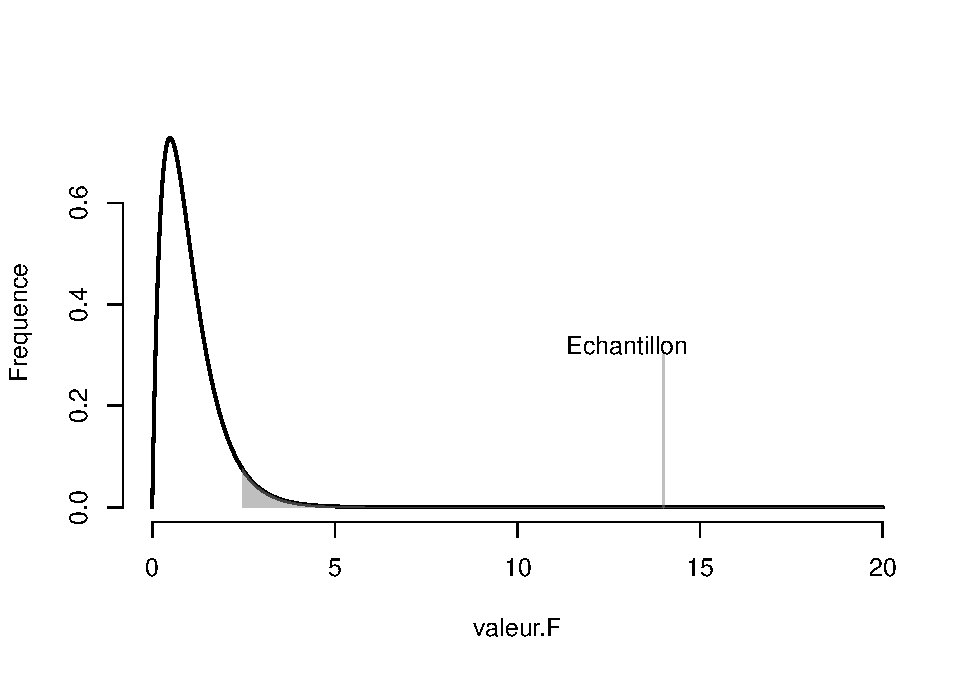
\includegraphics{04-Analyses_files/figure-latex/ft-1.pdf}
\caption{\label{fig:ft}Valeur-\(F\) de la comparaison des moyennes}
\end{figure}

\hypertarget{lassociation-linuxe9aire}{%
\section{L'association linéaire}\label{lassociation-linuxe9aire}}

\hypertarget{la-covariance}{%
\subsection{La covariance}\label{la-covariance}}

La covariance représente une mesure du degré auquel une variable augmente lorsque l'autre augmente. Elle correspond au produit moyen entre deux variables centrées (dont les moyennes sont soustraites). On retrouve l'équation sous la forme suivante.
\[\text{cov}_{xy} = \sigma_{xy}=\frac{1}{n-1}\sum_{i=1}^n(x_i-\bar{x})(y_i-\bar{y})\]

La covariance est une extension multivariée de la variance. La variance est le produit d'une variable \textbf{centrée} avec elle-même (le carré de la variable), \[\sigma^2=\frac{1}{n-1}\sum_{i=1}^nx_ix_i\].

En transformant \(x\) et \(y\) pour qu'elles soient \textbf{centrées}, l'aspect de produit entre les deux variables devient évident dans l'expression de la covariance.
\[\text{cov}_{xy} = \frac{1}{n-1}\sum_{i=1}^nxy\]
La programmation de la covariance pourrait se traduire ainsi.

\begin{Shaded}
\begin{Highlighting}[]
\NormalTok{covariance }\OtherTok{\textless{}{-}} \ControlFlowTok{function}\NormalTok{(x, y)\{}
  \CommentTok{\# X est une data.frame ou matrice de n sujets par p variables}
\NormalTok{  n }\OtherTok{\textless{}{-}} \FunctionTok{length}\NormalTok{(x)}
  \CommentTok{\# centrer variables}
\NormalTok{  xc }\OtherTok{\textless{}{-}}\NormalTok{ x }\SpecialCharTok{{-}} \FunctionTok{mean}\NormalTok{(x)}
\NormalTok{  yc }\OtherTok{\textless{}{-}}\NormalTok{ y }\SpecialCharTok{{-}} \FunctionTok{mean}\NormalTok{(y)}
\NormalTok{  prod.xy }\OtherTok{\textless{}{-}}\NormalTok{ xc }\SpecialCharTok{*}\NormalTok{ yc}
\NormalTok{  cov.xy }\OtherTok{\textless{}{-}} \FunctionTok{sum}\NormalTok{(prod.xy) }\SpecialCharTok{/}\NormalTok{ (n}\DecValTok{{-}1}\NormalTok{)}
  \FunctionTok{return}\NormalTok{(cov.xy)}
\NormalTok{\}}
\end{Highlighting}
\end{Shaded}

La fonction de base \texttt{cov()} sera plus efficace (plus robuste et plus simple) que la fonction maison précédente. La fonction \texttt{cov()} peut tenir compte de plus de deux variables.
La covariance indique la direction de la covariation entre les deux variables, positives ou négatives, mais n'indique pas la force de la relation. Bien qu'une covariance de 0 indique l'absence de colinéarité, une covariance de 120 n'est pas nécessairement plus forte qu'une covariance de 1. La mesure est intrinsèquement influencée par les unités l'échelle de mesure. Il serait aberrant de considérer le système métrique comme moins efficace, car ces mesures sont moins variables que les mesures impériales. (Il y a plusieurs raisons de préférer le système métrique, mais ce n'en est pas une!)

\hypertarget{la-corruxe9lation}{%
\subsection{La corrélation}\label{la-corruxe9lation}}

La corrélation représente le degré d'association linéaire entre deux variables. Une façon simple de considérer la corrélation est de la concevoir comme une covariance standardisée. Elle varie entre -1 et 1, ces deux dernières valeurs impliquant, respectivement, une relation parfaitement négative et positive entre les deux variables. En plus d'indiquer la direction de la relation, la corrélation suggère une force à ce lien. Lorsque la valeur de la corrélation est nulle, \(r=0\), un diagramme de dispersion ne montre qu'un nuage de point épars (sans structure), plus la corrélation augmente (en terme absolu) plus le nuage tends vers une ligne droite. La Figure \ref{fig:corimage} montre différentes valeurs de corrélation et un exemple de nuage de point qui lui est associé.

\begin{figure}

{\centering 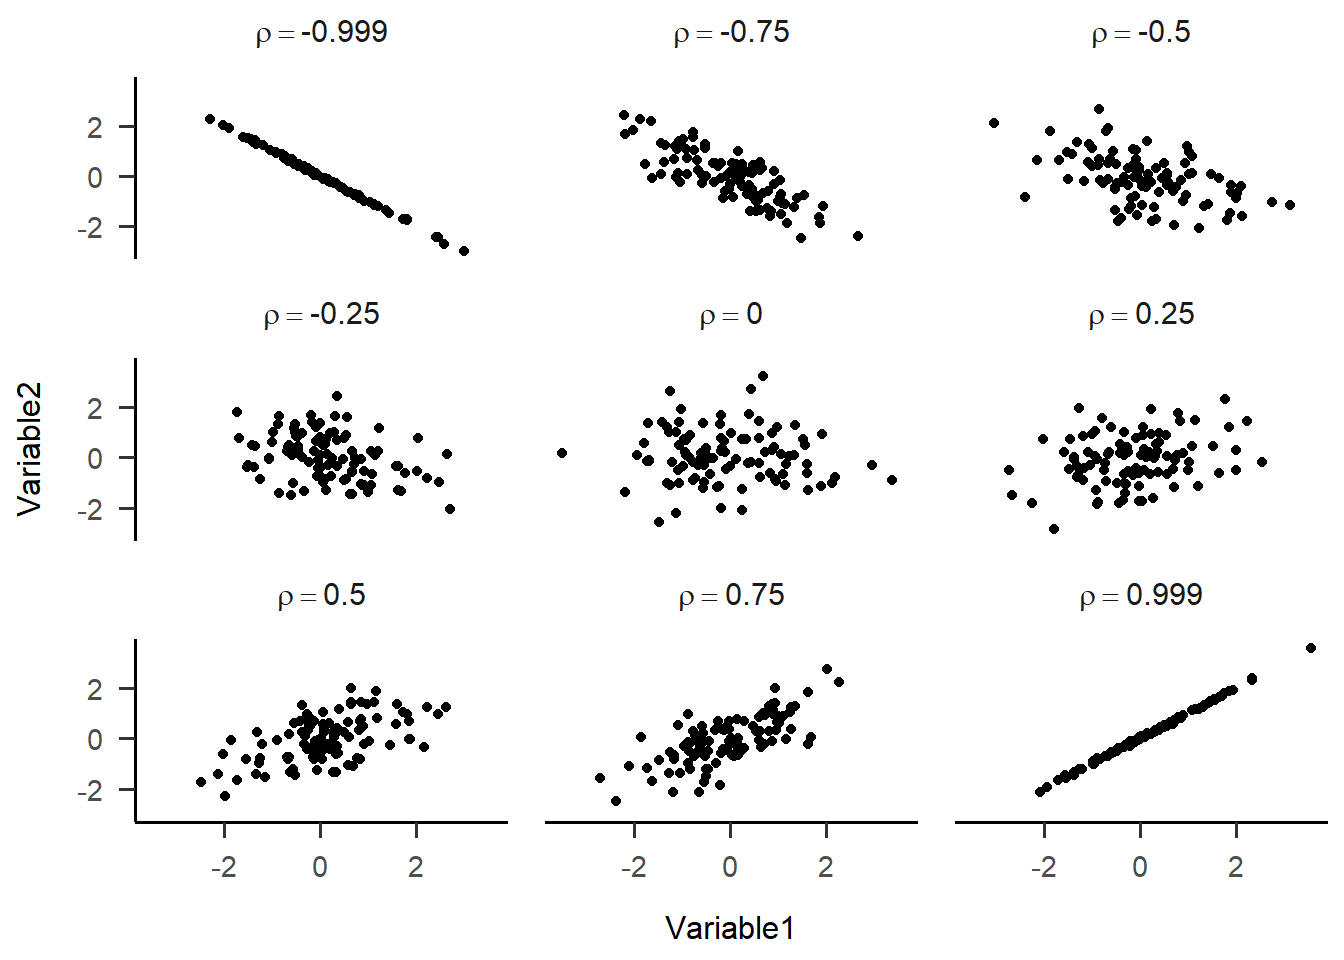
\includegraphics[width=0.5\linewidth,height=0.5\textheight]{04-Analyses_files/figure-latex/corimage-1} 

}

\caption{Illustrations de diagrammes de dispersion associé en fonction de corrélations}\label{fig:corimage}
\end{figure}

En statistiques, la corrélation est souvent représentée par la lettre grecque \(\rho\) (rho) ou l'usuel \(r\) lorsqu'il s'agit d'une estimation à partir d'un échantillon.

Il y a plusieurs méthodes pour calculer la corrélation. Une première est de considérer la corrélation comme le produit de variables standardisées (autrement dit, score-\(z\)). Pour la covariance, la moyenne était soustraite de la variable, donc des variables centrées. Pour la corrélation, on divise l'écart type également pour obtenir des variables standardisées.

En admettant que \(x\) et \(y\) sont déjà \textbf{standardisée}, \(z_x,z_y\), comme c'était le cas pour la covariance, l'aspect de produit entre les deux variables est conservé.
\[\text{cor}_{xy} = r_{xy}= \frac{1}{n-1}\sum_{i=1}^nz_xz_y\]

Il est possible de calculer la directement la corrélation à partir de la covariance, soit en divisant par le produit des écarts types des variables.

\[r_{xy} = \frac{\text{cov}_{xy}}{\sigma_x\sigma_y}\]

Voici trois options de programmation de la corrélation. La première et la deuxième sont basées sur la covariance. Dans la première, la covariance est calculée de nouveau dans la fonction. La deuxième quant à elle profite avantageusement de l'existence d'une fonction maison qui calcule directement la covariance. La troisième recourt au produit de variables standardisées.

\begin{Shaded}
\begin{Highlighting}[]
\CommentTok{\# Option 1 : Calcul complet}
\NormalTok{correlation1 }\OtherTok{\textless{}{-}} \ControlFlowTok{function}\NormalTok{(x, y)\{}
\NormalTok{  n }\OtherTok{\textless{}{-}} \FunctionTok{length}\NormalTok{(x)}
  \CommentTok{\# centrer variables}
\NormalTok{  xc }\OtherTok{\textless{}{-}}\NormalTok{ x }\SpecialCharTok{{-}} \FunctionTok{mean}\NormalTok{(x)}
\NormalTok{  yc }\OtherTok{\textless{}{-}}\NormalTok{ y }\SpecialCharTok{{-}} \FunctionTok{mean}\NormalTok{(y)}
\NormalTok{  prod.xy }\OtherTok{\textless{}{-}}\NormalTok{ xc }\SpecialCharTok{*}\NormalTok{ yc}
\NormalTok{  cov.xy }\OtherTok{\textless{}{-}} \FunctionTok{sum}\NormalTok{(prod.xy) }\SpecialCharTok{/}\NormalTok{ (n }\SpecialCharTok{{-}} \DecValTok{1}\NormalTok{)}
\NormalTok{  cor.xy }\OtherTok{\textless{}{-}}\NormalTok{ cov.xy }\SpecialCharTok{/}\NormalTok{ (}\FunctionTok{sd}\NormalTok{(x) }\SpecialCharTok{*} \FunctionTok{sd}\NormalTok{(y))}
  \FunctionTok{return}\NormalTok{(cor.xy)}
\NormalTok{\}}

\CommentTok{\# Option 2 : Basé sur la covariance}
\NormalTok{correlation2 }\OtherTok{\textless{}{-}} \ControlFlowTok{function}\NormalTok{(x, y)\{}
\NormalTok{  cov.xy }\OtherTok{\textless{}{-}} \FunctionTok{covariance}\NormalTok{(x,y) }
\NormalTok{  cor.xy }\OtherTok{\textless{}{-}}\NormalTok{ cov.xy }\SpecialCharTok{/}\NormalTok{ (}\FunctionTok{sd}\NormalTok{(x) }\SpecialCharTok{*} \FunctionTok{sd}\NormalTok{(y))}
  \FunctionTok{return}\NormalTok{(cor.xy)}
\NormalTok{\}}

\CommentTok{\# Option 3 : Basé sur des variables standardisées}
\NormalTok{correlation3 }\OtherTok{\textless{}{-}} \ControlFlowTok{function}\NormalTok{(x, y)\{}
\NormalTok{  n }\OtherTok{\textless{}{-}} \FunctionTok{length}\NormalTok{(x)}
\NormalTok{  xs }\OtherTok{\textless{}{-}}\NormalTok{ (x }\SpecialCharTok{{-}} \FunctionTok{mean}\NormalTok{(x)) }\SpecialCharTok{/} \FunctionTok{sd}\NormalTok{(x)}
\NormalTok{  ys }\OtherTok{\textless{}{-}}\NormalTok{ (y }\SpecialCharTok{{-}} \FunctionTok{mean}\NormalTok{(y)) }\SpecialCharTok{/} \FunctionTok{sd}\NormalTok{(y)}
\NormalTok{  cor.xy }\OtherTok{\textless{}{-}} \FunctionTok{sum}\NormalTok{(xs}\SpecialCharTok{*}\NormalTok{ys)}\SpecialCharTok{/}\NormalTok{(n }\SpecialCharTok{{-}} \DecValTok{1}\NormalTok{)}
  \FunctionTok{return}\NormalTok{(cor.xy)}
\NormalTok{\}}
\end{Highlighting}
\end{Shaded}

Évidemment, \textbf{R} possède une fonction de base pour le calcul d'une corrélation entre deux variables ou d'une matrice de corrélation (à partir d'un jeu de données de deux variables ou plus). Il s'agit de \texttt{cor()}. Ces trois fonctions maison en plus de la fonction \textbf{R} sont comparées ci-dessous. Pour ce faire, un jeu de données est créé possédant les caractéristiques désirées. Dans ce cas-ci, la taille d'échantillon est fixée à \(n=10000\) pour assurer une bonne précision dans l'échantillon et une corrélation \(r=.7\).

Une façon simple de produire des données à partir d'une matrice de corrélation (ou de covariance) est d'utiliser la fonction \texttt{mvrnorm()} du package \texttt{MASS}. Elle évitera pour l'instant d'introduire les manipulations mathématiques nécessaires (ce sera donc pour l'instant l'une de ces boîtes noires ayant la confiance de l'utilisateur). La fonction \texttt{mvrnorm()} pour \emph{MultiVariate Random NORMmal} nécessite trois arguments : La taille d'échantillon \texttt{n}, les moyennes \texttt{mu} des \(p\) variables et la matrice de covariance \texttt{Sigma} (la corrélation est un cas particulier de la covariance où les variables sont standardisées). Le lecteur avisé aura noté la ressemblance de nomenclature entre \texttt{mvrnorm()} (multivariée) et
\texttt{rnorm()} (univariée). Enfin, la dernière étape est de produire une matrice de covariance \(p \times p\). La fonction \texttt{matrix()} prend une variable de données, dans cet exemple , \texttt{c(1,\ r,\ r,\ 1)} qu'elle répartit ligne par colonne. Comme \(p=2\), cela crée une matrice \(2 \times 2\).

\begin{Shaded}
\begin{Highlighting}[]
\FunctionTok{set.seed}\NormalTok{(}\DecValTok{820}\NormalTok{)}
\CommentTok{\# Taille d\textquotesingle{}échantillon importante pour réduire l\textquotesingle{}erreur d\textquotesingle{}échantillonnage}
\NormalTok{n }\OtherTok{\textless{}{-}} \DecValTok{10000}
\CommentTok{\# La corrélation désirée}
\NormalTok{r }\OtherTok{\textless{}{-}}\NormalTok{ .}\DecValTok{70}
\CommentTok{\# Création d\textquotesingle{}une matrice de corrélation}
\NormalTok{R }\OtherTok{\textless{}{-}} \FunctionTok{matrix}\NormalTok{(}\FunctionTok{c}\NormalTok{(}\DecValTok{1}\NormalTok{, r, r, }\DecValTok{1}\NormalTok{), }\AttributeTok{nrow =} \DecValTok{2}\NormalTok{, }\AttributeTok{ncol =} \DecValTok{2}\NormalTok{)}
\CommentTok{\# Création des données }
\NormalTok{donnees }\OtherTok{\textless{}{-}} \FunctionTok{data.frame}\NormalTok{(MASS}\SpecialCharTok{::}\FunctionTok{mvrnorm}\NormalTok{(}\AttributeTok{n =}\NormalTok{ n, }\AttributeTok{mu =} \FunctionTok{c}\NormalTok{(}\DecValTok{0}\NormalTok{,}\DecValTok{0}\NormalTok{), }\AttributeTok{Sigma =}\NormalTok{ R))}
\FunctionTok{colnames}\NormalTok{(donnees) }\OtherTok{\textless{}{-}} \FunctionTok{c}\NormalTok{(}\StringTok{"x"}\NormalTok{, }\StringTok{"y"}\NormalTok{)}
\CommentTok{\# Voici la matrice de corrélation}
\NormalTok{R}
\CommentTok{\#\textgreater{}      [,1] [,2]}
\CommentTok{\#\textgreater{} [1,]  1.0  0.7}
\CommentTok{\#\textgreater{} [2,]  0.7  1.0}
\CommentTok{\# Voici une visualisation partielle des données}
\FunctionTok{head}\NormalTok{(donnees)}
\CommentTok{\#\textgreater{}        x      y}
\CommentTok{\#\textgreater{} 1  0.635  0.914}
\CommentTok{\#\textgreater{} 2 {-}0.193  0.360}
\CommentTok{\#\textgreater{} 3 {-}0.602 {-}1.213}
\CommentTok{\#\textgreater{} 4 {-}0.841 {-}0.986}
\CommentTok{\#\textgreater{} 5 {-}0.105 {-}1.771}
\CommentTok{\#\textgreater{} 6 {-}2.147 {-}1.590}
\CommentTok{\# Vérifications des variables}
\FunctionTok{mean}\NormalTok{(donnees}\SpecialCharTok{$}\NormalTok{x); }\FunctionTok{mean}\NormalTok{(donnees}\SpecialCharTok{$}\NormalTok{y); }\FunctionTok{sd}\NormalTok{(donnees}\SpecialCharTok{$}\NormalTok{x); }\FunctionTok{sd}\NormalTok{(donnees}\SpecialCharTok{$}\NormalTok{y)}
\CommentTok{\#\textgreater{} [1] {-}0.00578}
\CommentTok{\#\textgreater{} [1] {-}0.00531}
\CommentTok{\#\textgreater{} [1] 0.999}
\CommentTok{\#\textgreater{} [1] 1.01}
\CommentTok{\# Les résultats sont près des attentes}
\CommentTok{\# Vérifications de la corrélations}
\FunctionTok{cor}\NormalTok{(donnees}\SpecialCharTok{$}\NormalTok{x, donnees}\SpecialCharTok{$}\NormalTok{y)}
\CommentTok{\#\textgreater{} [1] 0.699}
\FunctionTok{correlation1}\NormalTok{(donnees}\SpecialCharTok{$}\NormalTok{x, donnees}\SpecialCharTok{$}\NormalTok{y)}
\CommentTok{\#\textgreater{} [1] 0.699}
\FunctionTok{correlation2}\NormalTok{(donnees}\SpecialCharTok{$}\NormalTok{x, donnees}\SpecialCharTok{$}\NormalTok{y)}
\CommentTok{\#\textgreater{} [1] 0.699}
\FunctionTok{correlation3}\NormalTok{(donnees}\SpecialCharTok{$}\NormalTok{x, donnees}\SpecialCharTok{$}\NormalTok{y)}
\CommentTok{\#\textgreater{} [1] 0.699}
\CommentTok{\# Les résultats sont près des attentes et identiques}
\end{Highlighting}
\end{Shaded}

Pour tester la probabilité d'obtenir cette valeur, la corrélation \(r\) peut se transformer monotonement en valeur-\(t\), ce qui permet de calculer des valeurs-\(p\) par la suite.

\[ t_{n-2} = \frac{r}{(\frac{\sqrt{1-r^2}}{\sqrt{n-2}})} \]
Cette formule se traduit simplement en code \textbf{R}.

\begin{Shaded}
\begin{Highlighting}[]
\CommentTok{\# Création d\textquotesingle{}une matrice de corrélation, }
\CommentTok{\# il pourrait également s\textquotesingle{}agir d\textquotesingle{}un vecteur ou d\textquotesingle{}un scalaire.}
\NormalTok{r }\OtherTok{\textless{}{-}} \FunctionTok{matrix}\NormalTok{(}\FunctionTok{c}\NormalTok{(}\DecValTok{1}\NormalTok{,.}\DecValTok{5}\NormalTok{,.}\DecValTok{4}\NormalTok{,.}\DecValTok{5}\NormalTok{,}\DecValTok{1}\NormalTok{,.}\DecValTok{3}\NormalTok{,.}\DecValTok{4}\NormalTok{,.}\DecValTok{3}\NormalTok{,}\DecValTok{1}\NormalTok{),}\DecValTok{3}\NormalTok{,}\DecValTok{3}\NormalTok{)}
\CommentTok{\# Nombre d\textquotesingle{}unités (valeur arbitraire ici)}
\NormalTok{n }\OtherTok{\textless{}{-}} \DecValTok{10}
\CommentTok{\# Valeurs t}
\NormalTok{vt }\OtherTok{\textless{}{-}}\NormalTok{ r }\SpecialCharTok{*} \FunctionTok{sqrt}\NormalTok{(n }\SpecialCharTok{{-}} \DecValTok{2}\NormalTok{) }\SpecialCharTok{/} \FunctionTok{sqrt}\NormalTok{(}\DecValTok{1} \SpecialCharTok{{-}}\NormalTok{ r }\SpecialCharTok{\^{}} \DecValTok{2}\NormalTok{)}
\CommentTok{\# Valeurs{-}p}
\NormalTok{vp }\OtherTok{\textless{}{-}}\NormalTok{ (}\DecValTok{1} \SpecialCharTok{{-}} \FunctionTok{pt}\NormalTok{(}\FunctionTok{abs}\NormalTok{(vt), }\AttributeTok{df =}\NormalTok{ n }\SpecialCharTok{{-}} \DecValTok{2}\NormalTok{)) }\SpecialCharTok{*} \DecValTok{2}
\NormalTok{vt ; vp}
\CommentTok{\#\textgreater{}      [,1]  [,2]  [,3]}
\CommentTok{\#\textgreater{} [1,]  Inf 1.633 1.234}
\CommentTok{\#\textgreater{} [2,] 1.63   Inf 0.889}
\CommentTok{\#\textgreater{} [3,] 1.23 0.889   Inf}
\CommentTok{\#\textgreater{}       [,1]  [,2]  [,3]}
\CommentTok{\#\textgreater{} [1,] 0.000 0.141 0.252}
\CommentTok{\#\textgreater{} [2,] 0.141 0.000 0.400}
\CommentTok{\#\textgreater{} [3,] 0.252 0.400 0.000}
\end{Highlighting}
\end{Shaded}

Dans le code ci-dessous, l'équation précédente est subtilement réarrangée pour être plus simple et élégante quoiqu'équivalente.
\[ t_{n-2} = \frac{r}{(\frac{\sqrt{1-r^2}}{\sqrt{n-2}})} = \frac{r\sqrt{n-2}}{\sqrt{1-r^2}}\]
La première a l'avantage de montrer la relation entre l'estimateur et l'erreur type alors que la seconde est moins encombrante.

\hypertarget{les-donnuxe9es-nominales}{%
\section{Les données nominales}\label{les-donnuxe9es-nominales}}

Jusqu'à présent, deux types d'association de données ont été présenté : une variable nominale (identifiant des groupes) avec une variable continue (différences de moyenne) et deux variables continues (association linéaire). Dans cette section, l'association entre deux variables nominales est présentée. Une façon de représenter l'association entre deux variables nominales est le tableau de contingence, soit l'illustration d'une distribution d'une variable (en ligne) pour chaque catégorie de l'autre (en colonne). En voici, un exemple.

\begin{table}[H]

\caption{\label{tab:TCCV}Tableau de contingence de la relation entre posséder une voiture et le climatoscepticisme}
\centering
\begin{tabular}[t]{lcc}
\toprule
\multicolumn{1}{c}{Climatosceptique} & \multicolumn{2}{c}{Voiture} \\
\cmidrule(l{3pt}r{3pt}){1-1} \cmidrule(l{3pt}r{3pt}){2-3}
  & non & oui\\
\midrule
non & 87 & 104\\
oui & 7 & 52\\
\bottomrule
\end{tabular}
\end{table}

Le tableau \ref{tab:TCCV} présente deux variables nominales (\texttt{climatosceptique}, à la verticale, et posséder une \texttt{voiture}, à l'horizontale) ayant chacune deux catégories (\texttt{oui} et \texttt{non}). Il montre les proportions \textbf{observées}. Ces variables sont-elles associées? Pour traiter cette question, les proportions attendues jouent un rôle crucial. En fait, l'hypothèse nulle sous la table de contingence postule que toutes les proportions du tableau de contingence sont indépendantes. Mathématiquement, il s'agit de postuler que les proportions d'une variable (en ligne ou en colonne) n'influencent pas celles de l'autre variable. Pour obtenir les proportions \textbf{théoriques}, les totaux des lignes et colonnes sont calculés ainsi que le grand total. La fréquence attendue d'une cellule est obtenue en calculant, pour chaque cellule, le produit de sa colonne et de sa ligne respective divisé par le grand total.

\[t_{ij} = \frac{\text{total}_i \times \text{total}_j}{\sum \text{total}}\]

L'équation ci-dessus illustre l'idée sous-jacente à la proportion attendue, \(t\) d'une cellule de ligne, \(i\), et colonne \(j\).

\begin{table}[H]

\caption{\label{tab:TCCV2}Tableau de contingence étendu avec les totaux}
\centering
\begin{tabular}[t]{lccc}
\toprule
\multicolumn{1}{c}{Climatosceptique} & \multicolumn{2}{c}{Voiture} & \multicolumn{1}{c}{Total} \\
\cmidrule(l{3pt}r{3pt}){1-1} \cmidrule(l{3pt}r{3pt}){2-3} \cmidrule(l{3pt}r{3pt}){4-4}
  & non & oui & \\
\midrule
non & 87 & 104 & 191\\
oui & 7 & 52 & 59\\
Total & 94 & 156 & 250\\
\bottomrule
\end{tabular}
\end{table}

\hypertarget{le-chi2-pour-table-de-contingence}{%
\subsection{\texorpdfstring{Le \(\chi^2\) pour table de contingence}{Le \textbackslash chi\^{}2 pour table de contingence}}\label{le-chi2-pour-table-de-contingence}}

Maintenant que la question statistique et que l'hypothèse nulle sont posées, comment mesurer le degré selon lequel les données s'écartent des attentes \emph{théoriques}. Le \(\chi^2\) (prononcé khi-carré) permet de calculer une telle mesure. Le \(\chi^2\) correspond à la distance entre une valeur observée et théorique au carré, pondérée par la valeur théorique.
\[ \chi^2_v = \sum_{i=1}^{l}\sum_{j=1}^c(\frac{(o_{ij}-t_{ij})^2}{t_{ij}})\]
où \(o\) correspond aux valeurs observées, \(t\) réfère aux valeurs théoriques, \(v\) représente les degrés de liberté et \(i\) et \(j\) les lignes et colonnes respectivement. Le degré de liberté est
\[v = (n_{\text{ligne}}-1)(n_{\text{colonne}}-1)\]

Si l'hypothèse nulle est vraie, les valeurs observées et théoriques devraient être très près. Le carré permet de calculer une distance euclidienne et le dénominateur pondère la distance. Comme l'analyse de variance, le test de \(\chi^2\) pour table de contingence est global, il n'informe pas d'où provient la dépendance, mais bien s'il y a au moins une dépendance.

\begin{Shaded}
\begin{Highlighting}[]
\NormalTok{khicarre }\OtherTok{\textless{}{-}} \ControlFlowTok{function}\NormalTok{(obs)\{}
  \CommentTok{\# Obs est une table de contingence}
  \CommentTok{\# Somme colonne}
\NormalTok{  SC }\OtherTok{\textless{}{-}} \FunctionTok{as.matrix}\NormalTok{(}\FunctionTok{colSums}\NormalTok{(obs))}
  \CommentTok{\# Somme ligne}
\NormalTok{  SL }\OtherTok{\textless{}{-}} \FunctionTok{as.matrix}\NormalTok{(}\FunctionTok{rowSums}\NormalTok{(obs))}
  \CommentTok{\# Grand total}
\NormalTok{  TT }\OtherTok{\textless{}{-}} \FunctionTok{sum}\NormalTok{(obs)}
  \CommentTok{\# Proportion théoriques}
\NormalTok{  theo }\OtherTok{\textless{}{-}}\NormalTok{ SL }\SpecialCharTok{\%*\%} \FunctionTok{t}\NormalTok{(SC) }\SpecialCharTok{/}\NormalTok{ TT}
  \CommentTok{\# khi carré}
\NormalTok{  khi2 }\OtherTok{\textless{}{-}} \FunctionTok{sum}\NormalTok{((obs }\SpecialCharTok{{-}}\NormalTok{ theo) }\SpecialCharTok{\^{}} \DecValTok{2} \SpecialCharTok{/}\NormalTok{ theo)}
\NormalTok{  dl }\OtherTok{\textless{}{-}}\NormalTok{ (}\FunctionTok{length}\NormalTok{(SL) }\SpecialCharTok{{-}} \DecValTok{1}\NormalTok{) }\SpecialCharTok{*}\NormalTok{ (}\FunctionTok{length}\NormalTok{(SC) }\SpecialCharTok{{-}} \DecValTok{1}\NormalTok{)}
\NormalTok{  vp }\OtherTok{\textless{}{-}} \DecValTok{1} \SpecialCharTok{{-}} \FunctionTok{pchisq}\NormalTok{(khi2, dl)}
  \CommentTok{\# Sortie}
\NormalTok{  statistiques }\OtherTok{\textless{}{-}} \FunctionTok{list}\NormalTok{(}\AttributeTok{khi2 =}\NormalTok{ khi2, }\AttributeTok{dl =}\NormalTok{ dl, }\AttributeTok{valeur.p =}\NormalTok{ vp)}
  \FunctionTok{return}\NormalTok{(statistiques)}
\NormalTok{\}}
\end{Highlighting}
\end{Shaded}

Il y a plusieurs techniques pour créer une base de données, l'essentiel étant de lier les proportions désirées. Ici, une variable sexe est créée avec 50-50\% de chance d'être l'un ou l'autre sexe. Par la suite, une proportion différente liée au sexe est utilisée pour générer la fréquence de consommation de tabac. La syntaxe sert principalement à identifier les valeurs \texttt{homme} et \texttt{femme} de la première variable pour en associer une valeur \texttt{tabac}.

\begin{Shaded}
\begin{Highlighting}[]
  \FunctionTok{set.seed}\NormalTok{(}\DecValTok{54}\NormalTok{)}
\NormalTok{  n }\OtherTok{\textless{}{-}} \DecValTok{100}
  \CommentTok{\# Première variable}
\NormalTok{  sexe }\OtherTok{\textless{}{-}} \FunctionTok{sample}\NormalTok{(}\FunctionTok{c}\NormalTok{(}\StringTok{"homme"}\NormalTok{,}\StringTok{"femme"}\NormalTok{), }
                \AttributeTok{size =}\NormalTok{ n, }
                \AttributeTok{replace =} \ConstantTok{TRUE}\NormalTok{, }
                \AttributeTok{prob =} \FunctionTok{c}\NormalTok{(.}\DecValTok{5}\NormalTok{,.}\DecValTok{5}\NormalTok{))}
\NormalTok{  tabac }\OtherTok{\textless{}{-}} \FunctionTok{rep}\NormalTok{(}\DecValTok{0}\NormalTok{, }\DecValTok{100}\NormalTok{)}
  \CommentTok{\# Proportions conditionnelles}
\NormalTok{  tabac[sexe }\SpecialCharTok{==} \StringTok{"femme"}\NormalTok{] }\OtherTok{\textless{}{-}} \FunctionTok{sample}\NormalTok{(}\FunctionTok{c}\NormalTok{(}\StringTok{"fumeur"}\NormalTok{,}\StringTok{"non{-}fumeur"}\NormalTok{), }
                                    \AttributeTok{size =} \FunctionTok{sum}\NormalTok{(sexe }\SpecialCharTok{==} \StringTok{"femme"}\NormalTok{), }
                                    \AttributeTok{replace =} \ConstantTok{TRUE}\NormalTok{, }
                                    \AttributeTok{prob =} \FunctionTok{c}\NormalTok{(.}\DecValTok{2}\NormalTok{,.}\DecValTok{8}\NormalTok{))}
\NormalTok{  tabac[sexe }\SpecialCharTok{==} \StringTok{"homme"}\NormalTok{] }\OtherTok{\textless{}{-}} \FunctionTok{sample}\NormalTok{(}\FunctionTok{c}\NormalTok{(}\StringTok{"fumeur"}\NormalTok{,}\StringTok{"non{-}fumeur"}\NormalTok{), }
                                    \AttributeTok{size =} \FunctionTok{sum}\NormalTok{(sexe }\SpecialCharTok{==} \StringTok{"homme"}\NormalTok{), }
                                    \AttributeTok{replace =} \ConstantTok{TRUE}\NormalTok{, }
                                    \AttributeTok{prob =} \FunctionTok{c}\NormalTok{(.}\DecValTok{1}\NormalTok{,.}\DecValTok{9}\NormalTok{))}
  \CommentTok{\#base données}
\NormalTok{  donnees }\OtherTok{\textless{}{-}} \FunctionTok{data.frame}\NormalTok{(sexe, tabac)}
  \FunctionTok{table}\NormalTok{(donnees)}
\CommentTok{\#\textgreater{}        tabac}
\CommentTok{\#\textgreater{} sexe    fumeur non{-}fumeur}
\CommentTok{\#\textgreater{}   femme      8         38}
\CommentTok{\#\textgreater{}   homme      4         50}
\end{Highlighting}
\end{Shaded}

La fonction \texttt{table()} de \textbf{R} génère une table de contingence. La fonction maison et deux méthodes de base \textbf{R} sont présentées et produisent les mêmes résultats pour le \(\chi^2\). Un autre, le test exact de Fisher est également présenté. Celui-ci est plus robuste, mais peut requérir plus intensive des ressources de l'ordianteur pour les grosses tables de contingences.

Le test du \(\chi^2\) est sujet à certains problèmes qu'il est important de considérer sans quoi l'interprétation pourra être faussée. Si la taille d'échantillon (le nombre d'unités d'observation observées est trop faible), alors le test est biaisé. Par exemple, trois lancers de pile ou face ne sont pas suffisants pour tester une hypothèse de khi-carré, le nombre de résultats différents est de 2, ce qui ne donne pas une approximation satisfaisante de la distribution d'échantillonnage. La convention est de dire qu'une fréquence théorique est trop petite si elle est plus petite que 5. Si ce n'est pas cas, des corrections ou d'autres options doivent être considérées.

Dans le présent exemple, bien que les fréquences attendues respectent les critères usuels, il peut être utile d'envisager un test plus robuste comme le test exact de Fisher ou le \(\chi^2\) avec correction de continuité. Le premier se commande avec la fonction \texttt{fisher.test()} et le second est la fonction par défaut de \texttt{chisq.test()}. Pour montrer l'équivalent entre la fonction \texttt{chisq.test()} et la fonction maison, l'option de correction est désactivée avec l'argument \texttt{correct\ =\ FALSE}.

\begin{Shaded}
\begin{Highlighting}[]
\CommentTok{\# Table de contingence}
\NormalTok{TC }\OtherTok{\textless{}{-}} \FunctionTok{table}\NormalTok{(donnees)}
\CommentTok{\# Fonction maison}
\FunctionTok{khicarre}\NormalTok{(TC)}
\CommentTok{\#\textgreater{} $khi2}
\CommentTok{\#\textgreater{} [1] 2.34}
\CommentTok{\#\textgreater{} }
\CommentTok{\#\textgreater{} $dl}
\CommentTok{\#\textgreater{} [1] 1}
\CommentTok{\#\textgreater{} }
\CommentTok{\#\textgreater{} $valeur.p}
\CommentTok{\#\textgreater{} [1] 0.126}

\CommentTok{\# Fonction de base}
\FunctionTok{summary}\NormalTok{(TC)}
\CommentTok{\#\textgreater{} Number of cases in table: 100 }
\CommentTok{\#\textgreater{} Number of factors: 2 }
\CommentTok{\#\textgreater{} Test for independence of all factors:}
\CommentTok{\#\textgreater{}  Chisq = 2.3, df = 1, p{-}value = 0.1}

\CommentTok{\# Autre fonction de base}
\NormalTok{resultat }\OtherTok{\textless{}{-}} \FunctionTok{chisq.test}\NormalTok{(TC, }\AttributeTok{correct =} \ConstantTok{FALSE}\NormalTok{)}
\NormalTok{resultat}
\CommentTok{\#\textgreater{} }
\CommentTok{\#\textgreater{}  Pearson\textquotesingle{}s Chi{-}squared test}
\CommentTok{\#\textgreater{} }
\CommentTok{\#\textgreater{} data:  TC}
\CommentTok{\#\textgreater{} X{-}squared = 2, df = 1, p{-}value = 0.1}

\CommentTok{\# Et pour plus de précision...}
\NormalTok{resultat}\SpecialCharTok{$}\NormalTok{statistic}
\CommentTok{\#\textgreater{} X{-}squared }
\CommentTok{\#\textgreater{}      2.34}
\NormalTok{resultat}\SpecialCharTok{$}\NormalTok{p.value}
\CommentTok{\#\textgreater{} [1] 0.126}

\CommentTok{\# Le test exact de Fisher}
\NormalTok{resultat.fisher }\OtherTok{\textless{}{-}} \FunctionTok{fisher.test}\NormalTok{(TC)}
\NormalTok{resultat.fisher}
\CommentTok{\#\textgreater{} }
\CommentTok{\#\textgreater{}  Fisher\textquotesingle{}s Exact Test for Count Data}
\CommentTok{\#\textgreater{} }
\CommentTok{\#\textgreater{} data:  TC}
\CommentTok{\#\textgreater{} p{-}value = 0.2}
\CommentTok{\#\textgreater{} alternative hypothesis: true odds ratio is not equal to 1}
\CommentTok{\#\textgreater{} 95 percent confidence interval:}
\CommentTok{\#\textgreater{}   0.641 12.731}
\CommentTok{\#\textgreater{} sample estimates:}
\CommentTok{\#\textgreater{} odds ratio }
\CommentTok{\#\textgreater{}       2.61}
\NormalTok{resultat.fisher}\SpecialCharTok{$}\NormalTok{p.value}
\CommentTok{\#\textgreater{} [1] 0.216}
\end{Highlighting}
\end{Shaded}

\hypertarget{exercice-analyse}{%
\chapter*{Exercices}\label{exercice-analyse}}
\addcontentsline{toc}{chapter}{Exercices}

TODO

\begin{enumerate}
\def\labelenumi{\arabic{enumi}.}
\item
  Créer une table de valeur-\(t\) critique pour \(dl = 1,2,3 ,... ,30\) et \(\alpha=.05\) unilatérale.
\item
  Comparer la puissance de la distribution-\(t\) par rapport à une distribution normale centrée réduite. La différence par rapport à l'hypothèse nulle est 2 et l'écart type est 1, l'\(\alpha = .05\) bilatérale. Tester pour différentes valeurs de \(n\).
\item
  Créer un jeu de données pour test-\(t\) dépendant avec une corrélation de .3 entre les temps de mesure, des variances de 1, une différence de moyenne de 1 et une taille d'échantillon \(n = 20\). Analyser ce jeu de données : vérifier la corrélation et la différence.
\item
  Calculer la puissance d'une corrélation de \(\rho = .30\) pour une taille d'échantillon \(n=80\) et \(alpha = .05\) bilatérale.
\item
  Comparer l'erreur de type I du test-\(t\) indépendant avec équivalence versus non-équivalence des variances pour une différence de moyennes de 1 et des variances de \(.25\) pour le groupe 1 et \(1\) pour le groupe 2 pour une taille d'échantillon de 30 séparé également entre les groupes.
\end{enumerate}

\hypertarget{techniques-avancuxe9es-de-moduxe9lisation}{%
\chapter{Techniques avancées de modélisation}\label{techniques-avancuxe9es-de-moduxe9lisation}}

Dans le chapitre sur la régression, les variables indépendantes sont créées simultanément à partir d'une matrice de corrélation. Dans un modèle plus élaboré, plutôt que d'ignorer ces corrélations, comme le fait l'analyse de régression, il est possible de modéliser explicitement les liens entre les variables prédictrices.

Cela revient à décrire un modèle de façon à ce qu'une première variable \emph{cause} la seconde; la première et la seconde \emph{causent} la troisième et ainsi de suite.

La modélisation en système d'équations deviendra primordial dans les prochaines sections, notamment pour les analyses de trajectoires, de médiation, de modération, et plus. C'est le fondement de la modélisation par équations structurelles (SEM).
Dans ce chapitre, des techniques de modélisation avancées sont présentées. Elles s'appliquent à des modèles de trajectoires récursifs, c'est-à-dire que la \emph{causation} s'enchaîne dans une direction, de la première variable vers la dernière.

\hypertarget{la-loi-de-la-somme-des-variances}{%
\section[La loi de la somme des variances]{\texorpdfstring{La loi de la somme des variances\footnote{La section est partiellement basée sur \textcite{Caron21}.}}{La loi de la somme des variances}}\label{la-loi-de-la-somme-des-variances}}

La loi de la somme des variances explique comment additionner la variance de variables aléatoires, quelle que soit leur distribution \autocite{casella2002}. Le cas le plus simple est celui de deux variables aléatoires, comme \(x_1\) et \(x_2\), et la façon dont elles s'additionnent pour former une troisième variable, \(y\). Elles donnent un modèle simple représenté par l'équation \eqref{eq:eq1}.

\begin{equation}
y=x_1+x_2
\label{eq:eq1}
\end{equation}

La variance de leur somme prend la forme suivante
\begin{equation}
\sigma_y^2=\sigma_{x_1}^2+\sigma_{x_2}^2
\label{eq:eq2}
\end{equation}

où \(\sigma^2\) est le symbole habituel de la variance. La variance de la somme (ou de la différence) de deux variables indépendantes (non-corrélées) aléatoires est leur somme. En fait, la somme de \(p\) variables indépendantes est la somme de leurs variances. En syntaxe \textbf{R}, ces équations ressemblent à ceci.

\begin{Shaded}
\begin{Highlighting}[]
\FunctionTok{set.seed}\NormalTok{(}\DecValTok{1155}\NormalTok{)                  }\CommentTok{\# reproductibilité}
\NormalTok{n }\OtherTok{\textless{}{-}} \DecValTok{100000}                      \CommentTok{\# taille élevée pour la précision}
\NormalTok{s.x1 }\OtherTok{\textless{}{-}} \FunctionTok{sqrt}\NormalTok{(}\DecValTok{2}\NormalTok{)                  }\CommentTok{\# variance de 2 }
\NormalTok{s.x2 }\OtherTok{\textless{}{-}} \FunctionTok{sqrt}\NormalTok{(}\DecValTok{3}\NormalTok{)                  }\CommentTok{\# variance de 3}

\CommentTok{\# Création des variables}
\NormalTok{x1 }\OtherTok{\textless{}{-}} \FunctionTok{rnorm}\NormalTok{(}\AttributeTok{n =}\NormalTok{ n, }\AttributeTok{sd =}\NormalTok{ s.x1) }
\NormalTok{x2 }\OtherTok{\textless{}{-}} \FunctionTok{rnorm}\NormalTok{(}\AttributeTok{n =}\NormalTok{ n, }\AttributeTok{sd =}\NormalTok{ s.x2)     }
\end{Highlighting}
\end{Shaded}

Dans cet exemple, les variances de \texttt{x1} et de \texttt{x3} sont égales à 2 et 3 respectivement. Si ces deux variables sont additionnées pour créer \texttt{y}, l'équation \eqref{eq:eq2} implique que la variance est de \(\sigma^2_{x_{1}} + \sigma^2_{x_2} = 2 + 3= 5\)

\begin{Shaded}
\begin{Highlighting}[]
\NormalTok{y }\OtherTok{\textless{}{-}}\NormalTok{ x1 }\SpecialCharTok{+}\NormalTok{ x2}
\FunctionTok{var}\NormalTok{(y)}
\CommentTok{\#\textgreater{} [1] 5}

\CommentTok{\# Vérifier par}
\NormalTok{s.x1}\SpecialCharTok{\^{}}\DecValTok{2} \SpecialCharTok{+}\NormalTok{ s.x2}\SpecialCharTok{\^{}}\DecValTok{2}
\CommentTok{\#\textgreater{} [1] 5}
\end{Highlighting}
\end{Shaded}

Le résultat concorde.

En pratique, il est rare que les variables prédictrices soient non corrélées. Ici, aucune corrélation n'a été précisée entre \texttt{x1} et \texttt{x2}. En développant le cas général où les variables sont corrélées, si la covariance entre \(x_1\) et \(x_2\) est \(\sigma_{x_1,x_2}\), alors la loi de la somme des variances devient ceci.

\begin{equation}
\sigma_y^2=\sigma_{x_1}^2+\sigma_{x_2}^2+2\sigma_{x_1,x_2}
\label{eq:eq3}
\end{equation}

L'équation \eqref{eq:eq2} est un cas particulier lorsque \(\sigma_{x_1 x_2}=0\). En syntaxe \textbf{R}, pour \(\rho = .5\), cela revient à programmer ceci.

\begin{Shaded}
\begin{Highlighting}[]
\CommentTok{\# Création de variables corrélées}
\NormalTok{rho }\OtherTok{\textless{}{-}}\NormalTok{ .}\DecValTok{5}                          \CommentTok{\# corrélation de .5}
\NormalTok{s.x1x2 }\OtherTok{\textless{}{-}}\NormalTok{ rho }\SpecialCharTok{*}\NormalTok{ s.x1 }\SpecialCharTok{*}\NormalTok{ s.x2        }\CommentTok{\# covariance de x et y}
\NormalTok{S }\OtherTok{\textless{}{-}} \FunctionTok{matrix}\NormalTok{(}\FunctionTok{c}\NormalTok{(s.x1}\SpecialCharTok{\^{}}\DecValTok{2}\NormalTok{, s.x1x2,      }\CommentTok{\# matrice de covariance}
\NormalTok{             s.x1x2, s.x2}\SpecialCharTok{\^{}}\DecValTok{2}\NormalTok{), }\AttributeTok{ncol =}  \DecValTok{2}\NormalTok{, }\AttributeTok{nrow =} \DecValTok{2}\NormalTok{)}

\CommentTok{\# Création de variables}
\NormalTok{X }\OtherTok{\textless{}{-}}\NormalTok{ MASS}\SpecialCharTok{::}\FunctionTok{mvrnorm}\NormalTok{(}\AttributeTok{n =}\NormalTok{ n, }\AttributeTok{Sigma =}\NormalTok{ S, }\AttributeTok{mu =} \FunctionTok{c}\NormalTok{(}\DecValTok{0}\NormalTok{, }\DecValTok{0}\NormalTok{), }\AttributeTok{empirical =} \ConstantTok{TRUE}\NormalTok{)}
\NormalTok{x1 }\OtherTok{\textless{}{-}}\NormalTok{ X[,}\DecValTok{1}\NormalTok{] ; x2 }\OtherTok{\textless{}{-}}\NormalTok{ X[,}\DecValTok{2}\NormalTok{]}

\CommentTok{\# La somme de deux variables corrélées}
\NormalTok{y }\OtherTok{\textless{}{-}}\NormalTok{ x1 }\SpecialCharTok{+}\NormalTok{ x2}
\FunctionTok{var}\NormalTok{(y)}
\CommentTok{\#\textgreater{} [1] 7.45}

\CommentTok{\# Vérifier par}
\NormalTok{s.x1}\SpecialCharTok{\^{}}\DecValTok{2} \SpecialCharTok{+}\NormalTok{ s.x2}\SpecialCharTok{\^{}}\DecValTok{2} \SpecialCharTok{+} \DecValTok{2} \SpecialCharTok{*}\NormalTok{ s.x1x2}
\CommentTok{\#\textgreater{} [1] 7.45}
\end{Highlighting}
\end{Shaded}

Pour rappel, la corrélation s'obtient avec \(\rho_{x_1,x_2}=\sigma_{x_1,x_2}/(\sigma_{x_1} \sigma_{x_2})\) et inversement la covariance est obtenue par \(\rho_{x_1,x_2} \sigma_{x_1} \sigma_{x_2}=\sigma_{x_1,x_2}\). En calculant la covariance d'abord, soit

\[\sigma_{x_1,x_2} = \rho_{x_1,x_2} \sigma_{x_1} \sigma_{x_2} = 0.5 \times 1.414 \times 1.732 = 1.225\]
et confirmé par \textbf{R}.

\begin{Shaded}
\begin{Highlighting}[]
\NormalTok{s.x1x2}
\CommentTok{\#\textgreater{} [1] 1.22}
\end{Highlighting}
\end{Shaded}

L'équation \eqref{eq:eq3} pour la variance de \texttt{y} mène à

\[\sigma_y^2=\sigma_{x_1}^2+\sigma_{x_2}^2+2\sigma_{x_1,x_2}= 2+3 + 2 \times 1.225  = 7.449\]
très près du 7.449 simulé.

La loi des sommes des variances est directement reliée au théorème de Pythagore tel qu'illustré par l'équation \eqref{eq:eq2}. Deux variables non corrélées peuvent être envisagées comme formant un triangle rectangle. L'équation \eqref{eq:eq3} est la règle du cosinus, ou la généralisation du théorème de Pythagore pour les triangles non rectangulaires, de sorte que la corrélation représente géométriquement un angle \autocite{Rodgers88}.

La Figure \ref{fig:tri1111} montre un triangle rectangle dont l'hypoténuse représente l'écart type de la somme de deux variables indépendantes. Lorsque l'angle est à 90\(^\circ\), la corrélation est nulle. Il suffit de mettre les droites au carré pour retrouver l'équation \eqref{eq:eq2}. Lorsque l'angle rétréci, plus les deux lignes \(\sigma\) se rapprochent et projettent sur une plus longue distance la somme des variances. Lorsqu'elles sont collées l'une sur l'autre, la corrélation est parfaite.

\begin{figure}

{\centering 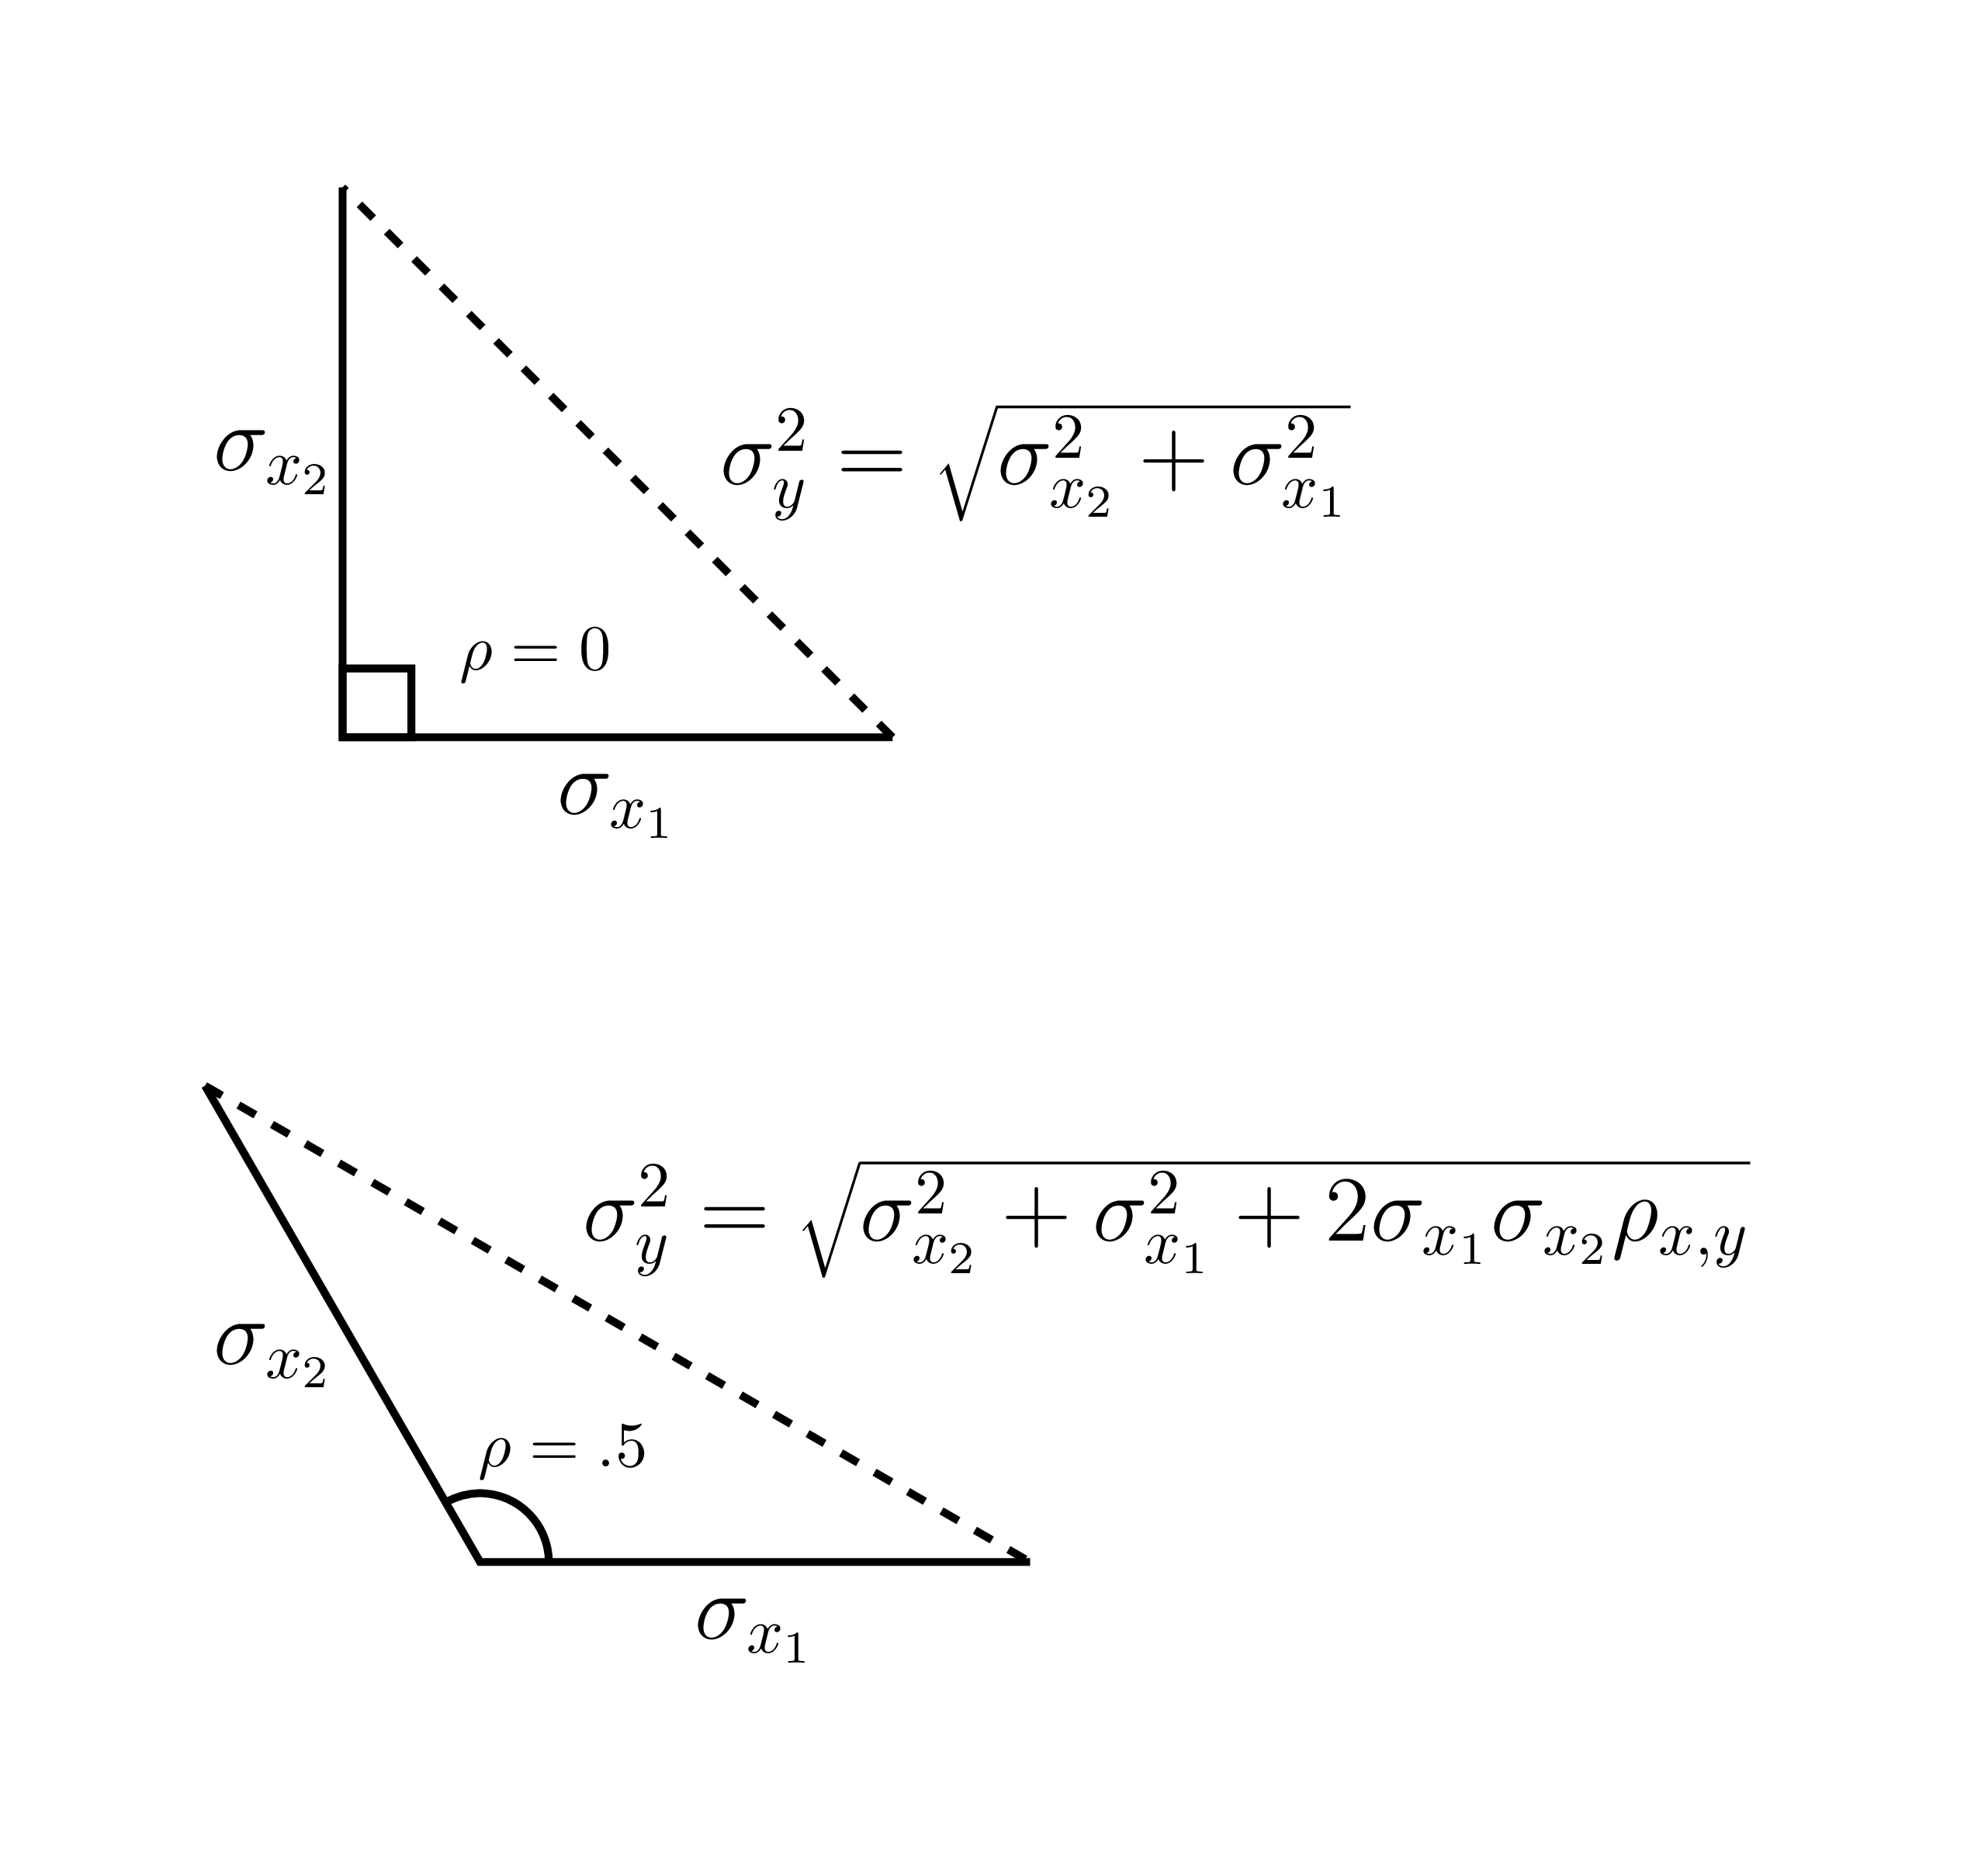
\includegraphics[width=0.75\linewidth,height=0.75\textheight]{image//tri} 

}

\caption{Représentation des variables sous forme de triangles}\label{fig:tri1111}
\end{figure}

Une autre façon plus mathématiquement simple est de calculer la loi de la somme des variances est de concevoir la variance de la somme de \(p\) variables comme la \emph{grande somme} de leur matrice de covariance. La grande somme est une fonction mathématique informelle qui fait référence à la somme de tous les éléments d'une matrice. Soit \(\mathbf{\Sigma}\), la matrice de variance-covariance de deux variables aléatoires \(x_1\) et \(x_2\) (les éléments diagonaux sont des variances), alors

\begin{equation}
\sigma_y^2 = \text{grande somme}(\mathbf{\Sigma}) = \text{grande somme}\left(\begin{array}{cc}
\sigma_{x_1}^2 & \sigma_{x_1,x_2} \\
\sigma_{x_1,x_2} & \sigma_{x_2}^2
\end{array}\right)
\label{eq:eq4}
\end{equation}

ce qui, en faisant la somme, conduit à l'équation \eqref{eq:eq3}. Encore une fois, si \(\sigma_{x_1,x_2}=0\), alors l'équation \eqref{eq:eq4} est égale à l'équation \eqref{eq:eq2}. Cette formulation a l'avantage de montrer l'origine des deux covariances dans l'équation \eqref{eq:eq3}. En code \textbf{R}, la syntaxe est dès plus rudimentaire.

\begin{Shaded}
\begin{Highlighting}[]
\FunctionTok{sum}\NormalTok{(S)}
\CommentTok{\#\textgreater{} [1] 7.45}
\end{Highlighting}
\end{Shaded}

Même si la notation matricielle peut sembler peu attrayante au départ, elle devient beaucoup plus intéressante lorsque le nombre de variables, \(p\), augmente, car il y a \(p(p-1)/2\) éléments hors diagonale à ajouter aux \(p\) variances. Elle deviendra même indispensable à la fin de ce chapitre.

Pour un exemple à \(p=3\), l'équation \eqref{eq:eq4} devient ceci.

\begin{equation}
\sigma_y^2=\text{grand somme}(\mathbf{\Sigma})=\text{grand somme}
\left(\begin{array}{ccc}
\sigma_{x_1}^2&\sigma_{x_1,x_2}&\sigma_{x_1 x_3} \\
\sigma_{x_1,x_2}&\sigma_{x_2}^2&\sigma_{x_2 x_3}\\
\sigma_{x_1 x_3}&\sigma_{x_2 x_3}&\sigma_{x_3}^2
\end{array}
\right)
\label{eq:eq5}
\end{equation}

Sous la forme linéaire, l'équation \eqref{eq:eq5} devient

\begin{equation}
\sigma_y^2=\sigma_{x_1}^2+\sigma_{x_2}^2+\sigma_{x_3}^2+2\sigma_{x_1,x_2}+2\sigma_{x_1 x_3}+2\sigma_{x_2 x_3}
\label{eq:eq6}
\end{equation}

et augmente à mesure que \(p\) s'accroît.

Une opération matricielle équivalente à la grande somme est

\begin{equation}
\mathbf{1}^{\prime} \mathbf{\Sigma} \mathbf{1}
\label{eq:GS}
\end{equation}

où \(1\) est un vecteur de longueur \(p\) contenant seulement 1. Voici en syntaxe \textbf{R}.

\begin{Shaded}
\begin{Highlighting}[]
\NormalTok{Un }\OtherTok{=} \FunctionTok{c}\NormalTok{(}\DecValTok{1}\NormalTok{, }\DecValTok{1}\NormalTok{)        }\CommentTok{\# Création du vecteur 1}
\FunctionTok{t}\NormalTok{(Un) }\SpecialCharTok{\%*\%}\NormalTok{ S }\SpecialCharTok{\%*\%}\NormalTok{ Un  }\CommentTok{\# Grande somme}
\CommentTok{\#\textgreater{}      [,1]}
\CommentTok{\#\textgreater{} [1,] 7.45}
\end{Highlighting}
\end{Shaded}

Cette opération produit la somme de tous les éléments de \(\mathbf{\Sigma}\) (\texttt{Sigma}). Cela sera utile pour dériver un cas plus général dans la section suivante.

\hypertarget{ajout-des-constantes-duxe9chelle-beta}{%
\subsection{\texorpdfstring{Ajout des constantes d'échelle \(\beta\)}{Ajout des constantes d'échelle \textbackslash beta}}\label{ajout-des-constantes-duxe9chelle-beta}}

Les équations \eqref{eq:eq3}, \eqref{eq:eq4}, \eqref{eq:eq5} et \eqref{eq:eq6} sont des cas particuliers d'une loi plus générale. Elles ne fonctionneraient pas si des constantes d'échelle (\emph{scaling constant}) étaient ajoutées (qui seront plus tard des coefficients de régression) ou pour calculer la différence (un type d'échelle également).

La situation où la variable \(y\) correspond au produit d'une constante \(\beta\) et de la variable \(x\) comme :

\begin{equation}
y=\beta x
\label{eq:eq7}
\end{equation}

un modèle linéaire qui ne comporte pas d'erreur (\(\epsilon\) est ignoré pour l'instant).

Il peut être utile de considérer \(\beta\) comme, éventuellement, le degré de relation entre deux variances, mais aussi comme un pur modificateur de l'écart type (également une constante d'échelle). De la même manière, une variable aléatoire avec une moyenne de \(0\) et un écart type de \(1\), \(x\sim \mathcal{N}(0,1)\), multipliée par la valeur \(\beta\), un facteur d'échelle arbitraire, devient distribuée comme \(\beta x \sim \mathcal{N}(0,\beta)\). Ainsi, \(\beta\) a modifié (ou mis à l'échelle) l'écart type de la distribution. Un cas connexe et fréquemment rencontré est lorsque les données sont normalisées en tant que score-\(z\) ou non normalisées (divisées ou multipliées respectivement par \(\sigma\)). La contribution est un écart-type, donc \(\beta\) doit être élevé au carré pour donner la variance de \(y\), soit \(\beta^2\). Cela mène à l'équation \eqref{eq:eq8} qui permet le calcul de la variance de \(y\).

\begin{equation}
\sigma_y^2=\beta^2 \sigma_x^2
\label{eq:eq8}
\end{equation}

En termes de syntaxe \textbf{R}, cela se traduit (toujours avec le même exemple).

\begin{Shaded}
\begin{Highlighting}[]
\NormalTok{beta }\OtherTok{=} \DecValTok{4}
\CommentTok{\# La variance de x1 est toujours de 2}
\NormalTok{y }\OtherTok{=}\NormalTok{ beta }\SpecialCharTok{*}\NormalTok{ x1}
\FunctionTok{var}\NormalTok{(y)}
\CommentTok{\#\textgreater{} [1] 32}

\CommentTok{\# Vérifier par}
\NormalTok{beta}\SpecialCharTok{\^{}}\DecValTok{2} \SpecialCharTok{*}\NormalTok{ s.x1}\SpecialCharTok{\^{}}\DecValTok{2}
\CommentTok{\#\textgreater{} [1] 32}
\end{Highlighting}
\end{Shaded}

L'équation \eqref{eq:eq8} donne \(\sigma_y^2=\beta^2 \sigma_x^2=4^2 \times 2= 32\), ce qui est identique.

L'étape suivante consiste à considérer un modèle avec deux variables et deux constantes d'échelles, ce qui rappelle de plus en plus la régression. Le modèle linéaire prend la forme suivante

\begin{equation}
y=\beta_1 x_1+\beta_2 x_2
\label{eq:eq9}
\end{equation}

qui est le même modèle que l'équation \eqref{eq:eq1} où les constantes d'échelle \(\beta_i\) sont ajoutées. Pour considérer les constantes d'échelle, la loi de la somme des variances basée sur l'équation \eqref{eq:eq2} devient pour deux variables indépendantes

\[
\sigma_y^2=\beta_1^2 \sigma_{x_1}^2+\beta_2^2 \sigma_{x_2}^2
\]

et quand ils covarient, comme l'équation \eqref{eq:eq3}, cela devient

\begin{equation}
\sigma_y^2=\beta_1^2 \sigma_{x_1}^2+\beta_2^2 \sigma_{x_2}^2+2\beta_1 \beta_2 \sigma_{x_1,x_2}
\label{eq:eq11}
\end{equation}

Dans ces équations, les \(\beta_i\) mettent à l'échelle la variance et la covariance. Ces équations se vérifient avec \textbf{R} (toujours avec le même exemple).

\begin{Shaded}
\begin{Highlighting}[]
\CommentTok{\# En suivant, l\textquotesingle{}exemple précédent}
\NormalTok{beta1 }\OtherTok{=} \DecValTok{4}
\NormalTok{beta2 }\OtherTok{=} \DecValTok{5}
\NormalTok{y }\OtherTok{=}\NormalTok{ beta1 }\SpecialCharTok{*}\NormalTok{ x1 }\SpecialCharTok{+}\NormalTok{ beta2 }\SpecialCharTok{*}\NormalTok{ x2}
\FunctionTok{var}\NormalTok{(y) }
\CommentTok{\#\textgreater{} [1] 156}

\CommentTok{\# Vérifier par}
\NormalTok{beta1}\SpecialCharTok{\^{}}\DecValTok{2} \SpecialCharTok{*}\NormalTok{ s.x1}\SpecialCharTok{\^{}}\DecValTok{2} \SpecialCharTok{+}\NormalTok{ beta2}\SpecialCharTok{\^{}}\DecValTok{2} \SpecialCharTok{*}\NormalTok{ s.x2}\SpecialCharTok{\^{}}\DecValTok{2} \SpecialCharTok{+} \DecValTok{2} \SpecialCharTok{*}\NormalTok{ beta1 }\SpecialCharTok{*}\NormalTok{ beta2 }\SpecialCharTok{*}\NormalTok{ s.x1x2 }
\CommentTok{\#\textgreater{} [1] 156}
\end{Highlighting}
\end{Shaded}

tel qu'attendue par l'équation \eqref{eq:eq12}.

\[
\sigma_y^2=\beta_1^2 \sigma_{x_1}^2+\beta_2^2 \sigma_{x_2}^2+2\beta_1 \beta_2 \sigma_{x_1,x_2} =
4^2 \times 2 + 5^2 \times 3 + 2 \times 4 \times 5 \times 1.225 = 155.99
\]

Comme précédemment, la formule en termes d'algèbre matricielle est plus simple et plus élégante, soit

\begin{equation}
\sigma_y^2 = \mathbf{B}^{\prime} \mathbf{\Sigma} \mathbf{B}
\label{eq:eq12}
\end{equation}

où \(\mathbf{B}\) (\(\beta\) majuscule) est un vecteur contenant tous les coefficients de régression \(\beta_i\) de longueur \(p\) prédisant \(y\) et s'appliquant à un nombre quelconque de prédicteurs \(x\). Le premier \(\prime\) est le symbole de transposition, un opérateur qui pivote la matrice sur sa diagonale et, dans le cas d'un vecteur, retourne les colonnes en lignes et vice-versa (voir son implication dans l'équation \eqref{eq:eq13} par exemple). Dans l'équation \eqref{eq:eq12}, utiliser deux fois les deux vecteurs B revient à élever au carré \(\beta_i\). Si \(\mathbf{B}\) sont tous égaux à 1, alors l'équation \eqref{eq:eq12} est identique à la définition d'une grande somme, voir l'équation \eqref{eq:GS}. En syntaxe \textbf{R}, l'équation \eqref{eq:eq12} donne :

\begin{Shaded}
\begin{Highlighting}[]
\NormalTok{beta }\OtherTok{=} \FunctionTok{c}\NormalTok{(beta1, beta2) }\CommentTok{\# Joint beta1 et beta2 dans un vecteur}
\NormalTok{beta }\SpecialCharTok{\%*\%}\NormalTok{ S }\SpecialCharTok{\%*\%}\NormalTok{ beta }\CommentTok{\# S est la matrice de covariance calculée auparavant.}
\CommentTok{\#\textgreater{}      [,1]}
\CommentTok{\#\textgreater{} [1,]  156}
\end{Highlighting}
\end{Shaded}

un code plus général et qui s'appliquera à toutes les situations (peu importe la valeur de \(p\), le nombre de variables).

Enfin, il est intéressant de noter que l'équation \eqref{eq:eq12} est la même que les coefficients de détermination, \(R^2\) \autocite{Cohen03}, lorsque toutes les variables et les coefficients de régression sont normalisés.

Dans le modèle linéaire simple décrit dans l'équation \eqref{eq:eq9}, l'équation \eqref{eq:eq11} devient :

\begin{equation}
\sigma_y^2 = 
\left(\begin{array}{cc} 
\beta_1 & \beta_2 
\end{array}\right) 
\left( \begin{array}{cc}
\sigma^2_{x_1} & \sigma_{x_1,x_2} \\
\sigma_{x_2,x_1} & \sigma^2_{x_2} 
\end{array} 
\right)
\left(\begin{array}{c} \beta_1 \\ \beta_2 \end{array} \right)
\label{eq:eq13}
\end{equation}

ce qui est équivalent à l'équation \eqref{eq:eq11}. À ce stade, le lecteur peut avoir l'intuition que les équations \eqref{eq:eq1} à \eqref{eq:eq6} n'étaient qu'un cas particulier où tous les \(\beta=1\).

La variance de la différence de deux variables revient à affirmer que le \(\beta\) des variables soustraites est de signe inverse(s'il est négatif, il devient positif ou s'il est positif, il devient négatif), c'est-à-dire \(-\beta\), ce qui pour le modèle conduit à

\[
y=\beta_1 x_1-\beta_2 x_2
\]

ou, de manière équivalente

\[
y=(\beta_1) x_1+(-\beta_2) x_2
\]

donnent

\begin{equation}
\begin{aligned}
\sigma_y^2 &= 
\left(\begin{array}{cc} 
\beta_1 & -\beta_2 
\end{array}\right) 
\left( \begin{array}{cc}
\sigma^2_{x_1} & \sigma_{x_1,x_2} \\
\sigma_{x_2,x_1} & \sigma^2_{x_2} 
\end{array} 
\right)
\left(\begin{array}{c} \beta_1 \\ -\beta_2 \end{array} \right) \\[15pt]
& = \beta_1^2 \sigma_{x_1}^2+(-\beta_2)^2 \sigma^2_{x_2} + 2(\beta_1)(-\beta_2)\sigma_{x_1,x_2} \\[15pt]
& = \beta_1^2 \sigma_{x_1}^2+\beta_2^2 \sigma^2_{x_2} - 2\beta_1\beta_2\sigma_{x_1,x_2}
\end{aligned}
\label{eq:eq16} 
\end{equation}

Ainsi, la variance de la différence de deux variables aléatoires est la somme de leurs variances en soustrayant deux fois leur échelle de covariance par \(\beta\) comme prévu. Cela se vérifie avec \textbf{R}.

\begin{Shaded}
\begin{Highlighting}[]
\NormalTok{y }\OtherTok{=}\NormalTok{ beta1 }\SpecialCharTok{*}\NormalTok{ x1 }\SpecialCharTok{{-}}\NormalTok{ beta2 }\SpecialCharTok{*}\NormalTok{ x2}
\FunctionTok{var}\NormalTok{(y)}
\CommentTok{\#\textgreater{} [1] 58}

\CommentTok{\# Vérifier par}
\NormalTok{beta }\OtherTok{=} \FunctionTok{c}\NormalTok{(beta1, }\SpecialCharTok{{-}}\NormalTok{beta2)   }\CommentTok{\# Signe négatif, très important!}
\NormalTok{beta }\SpecialCharTok{\%*\%}\NormalTok{ S }\SpecialCharTok{\%*\%}\NormalTok{ beta       }\CommentTok{\# Forme matricielle}
\CommentTok{\#\textgreater{}      [,1]}
\CommentTok{\#\textgreater{} [1,]   58}
\end{Highlighting}
\end{Shaded}

\hypertarget{implications-pour-la-moduxe9lisation}{%
\section{Implications pour la modélisation}\label{implications-pour-la-moduxe9lisation}}

La loi de la somme des variances a de nombreuses implications dans la modélisation, en particulier si les données sont façonnées selon certaines caractéristiques souhaitables, comme dans les modèles linéaires. La régression linéaire est une approche permettant de modéliser des effets additifs (variables indépendantes, \(x_i\)) pour prédire une variable dépendante (\(y\)). La linéarité fait référence à la propriété d'une fonction d'être compatible avec l'addition et la mise à l'échelle. En tant que tel, il existe une relation directe entre les équations ci-dessus et le modèle linéaire :

\begin{equation}
y=\beta_1 x_1 + ... +\beta_p x_p+\epsilon
\label{eq:eq17}
\end{equation}

en omettant la constante \(\beta_0\), qui ne joue aucun rôle dans la variance de la variable dépendante et en ajoutant l'erreur, une variable indépendante particulière qui est supposée ne pas être liée à \(x\), avoir une moyenne de \(0\), un écart-type \(\sigma_\epsilon\). L'équation \eqref{eq:eq17} est la forme générale du modèle linéaire de l'équation \eqref{eq:eq1} et \eqref{eq:eq8} dans laquelle la variance de \(y\) est une fonction des variances-covariances des \(x\) pondérées par \(\beta\).

\hypertarget{calcul-de-la-variance-de-lerreur}{%
\subsection{Calcul de la variance de l'erreur}\label{calcul-de-la-variance-de-lerreur}}

En prenant le modèle linéaire le plus simple, soit à deux variables :

\begin{equation}
y=x+\epsilon
\label{eq:eq18}
\end{equation}

où \(\epsilon\) est le terme d'erreur résiduel. C'est le minimum pour construire un modèle bivarié. Il s'agit de la même somme bivariée que l'équation \eqref{eq:eq1}, mais \(x_2\) est remplacé \(\epsilon\) et défini comme indépendant de \(x_1\) (non corrélé). Sur la base de ce modèle, l'équation \eqref{eq:eq2} conduit à l'équation suivante.

\[
\sigma_y^2=\sigma_x^2+\sigma_\epsilon^2
\]

Dans la plupart des cas de modélisation de données, les variances \(\sigma_x^2\) et \(\sigma_y^2\) sont généralement spécifiées à l'avance plutôt que \(\sigma_\epsilon^2\) de sorte que le calcul a priori de la variance de l'erreur au lieu de faire varier les paramètres d'intérêt est plus pertinent. En réarrangeant l'équation \eqref{eq:eq18} pour isoler \(\epsilon\),

\[
\epsilon=y-x
\]

et en termes de variance

\[
\sigma_\epsilon^2=\sigma_y^2+\sigma_x^2-2\sigma_{x,y}
\]

où l'équation \eqref{eq:eq16} pour la forme en algèbre matricielle.

\[
\sigma_y^2 = 
\left(\begin{array}{cc} 
1 & -1
\end{array}\right) 
\left( \begin{array}{cc}
\sigma^2_{y} & \sigma_{x,y} \\
\sigma_{x,y} & \sigma^2_{x} 
\end{array} 
\right)
\left(\begin{array}{c} 1 \\ -1 \end{array} \right) =
\sigma^2_y + \sigma^2_x - 2\sigma_{x,y}
\]

\hypertarget{variance-des-erreurs-avec-beta}{%
\subsection{\texorpdfstring{Variance des erreurs avec \(\beta\)}{Variance des erreurs avec \textbackslash beta}}\label{variance-des-erreurs-avec-beta}}

Une préoccupation lors de la modélisation des données est de préserver les propriétés souhaitées du modèle dans les jeux de données comme la variance de l'erreur, les paramètres de régression, les covariances, etc. Après la variance du terme d'erreur, le dernier élément à considérer est les coefficients de régression, \(\beta\), autrement dit, le degré de la relation entre les variables indépendantes et dépendantes. À partir de l'équation \eqref{eq:eq18}, on ajoute la pente et l'erreur :

\[
y=\beta x+\epsilon
\]

La loi de la somme des variances pour ce modèle devient

\begin{equation}
\sigma_y^2=\beta^2 \sigma_x^2+\sigma_\epsilon^2 
\label{eq:eq24}
\end{equation}

Pour rappel, l'erreur n'est pas corrélée à la variable indépendante \(x_i\). Comme précédemment, la forme d'algèbre matricielle est plus simple et plus élégante :

\begin{equation}
\sigma_y^2 = \mathbf{B}^{\prime} \mathbf{\Sigma} \mathbf{B} + \sigma_\epsilon^2
\label{eq:eq25}
\end{equation}

où \(\beta\) est un vecteur contenant tous les coefficients de régression \(\beta\) prédisant \(y\) et s'applique à un nombre quelconque de prédicteurs \(x\). En profitant de l'indépendance du terme d'erreur, l'équation \eqref{eq:eq25} est réarrangée comme :

\begin{equation}
\sigma_\epsilon^2=\sigma_y^2 -\mathbf{B}^{\prime} \mathbf{\Sigma} \mathbf{B}
\label{eq:eq26}
\end{equation}

ce qui donne la variance du terme d'erreur. Sous une forme linéaire (pour une seule variable indépendante), il est possible de réarranger l'équation \eqref{eq:eq24} pour isoler \(\sigma_\epsilon\).

\[
\sigma_\epsilon^2=\sigma_y^2-\beta^2 \sigma_x^2
\]

\hypertarget{le-scuxe9nario-standardisuxe9}{%
\subsection{Le scénario standardisé}\label{le-scuxe9nario-standardisuxe9}}

Pour conclure cette section, le scénario standardisé, c'est-à-dire lorsque les variances des variables sont égales à \(1\). Plus précisément, la variance de chaque variable est fixe ; seules les erreurs résiduelles doivent être ajustées pour maintenir ces propriétés. Dans ce scénario, la matrice de variance-covariance, \(\Sigma\), est une matrice de corrélation, qui définit les variances des erreurs résiduelles. Pour calculer la variance des erreurs des variables, l'équation \eqref{eq:eq26} est utilisée en remplaçant la variance des variables par \(1\) comme suit

\begin{equation}
\sigma_\epsilon^2=1 - \mathbf{B}^{\prime} \mathbf{\Sigma} \mathbf{B}
\label{eq:eq28}
\end{equation}

ou, pour un seul prédicteur.

\begin{equation}
\sigma_\epsilon^2=1-\beta^2 \sigma_x^2
\label{eq:eq29}
\end{equation}

Comme mentionner précédemment à propos de l'équation \eqref{eq:eq12}, ces deux dernières équations rappellent le coefficient de détermination. La valeur \(1\) correspond au potentiel explicatif d'une variable, \(\sigma_\epsilon^2\) est la variance résiduelle et, par conséquent, \(1-\sigma_\epsilon^2\) est la variance expliquée par le modèle.

\hypertarget{le-scuxe9nario-non-standardisuxe9}{%
\section{Le scénario non standardisé}\label{le-scuxe9nario-non-standardisuxe9}}

Dans la pratique, les scénarios sont rarement standardisés. Les variables n'ont pas toutes des variances de \(1\) et des moyennes de \(0\). Pour ajouter une touche de naturelle aux jeux de données, il est possible, une fois que le système d'équations est complètement obtenu, d'ajouter des variances différentes en multipliant une variable par l'écart-type souhaité et d'additionner un moyenne. Cela modifiera la matrice de covariance et les coefficients de régression, mais la force relative des liens et la matrice de corrélation resteront identiques. En d'autres termes, la \emph{déstandardisation} est l'inverse d'un score \(z\). Les données créées jusqu'ici sont des scores \(z\) et pour les déstandardisés, il faut procéder ainsi \(x = s(z + \bar{x})\), où \(s\) est l'écart-type et \(\bar{x}\) est la moyenne de la variable déstandardisée.

\hypertarget{cruxe9ation-de-variables-en-suxe9rie}{%
\section{Création de variables en série}\label{cruxe9ation-de-variables-en-suxe9rie}}

Jusqu'à présent, seule la création d'une variable est présentée. Le défi pour créer un système d'équations est d'obtenir la matrice de covariance des variables précédentes pour chaque variable subséquente.

Puisque le sujet peut devenir compliqué rapidement, cette section est basée sur un exemple à trois variables avec un scénario standardisé (variables centrées et réduites). Le cas général sera développé par la suite.

\hypertarget{cas-spuxe9cifique}{%
\subsection{Cas spécifique}\label{cas-spuxe9cifique}}

Le défi comment lorsqu'il y a trois ou plus variables à générer. Le cas à trois variables est tout de même abordable. La \emph{causalité} est unidirectionnelle, c'est-à-dire d'une variable vers une autre, sans retour en arrière. Cela se nomme un modèle récursif, impliquant du même coup l'existence de modèles non-récursifs, mais qui ne sont pas abordés. Pour un modèle à trois variables, une seule configuration récursive complète est possible. Elle est présentée à la Figure \ref{fig:mod3}.

\begin{figure}

{\centering 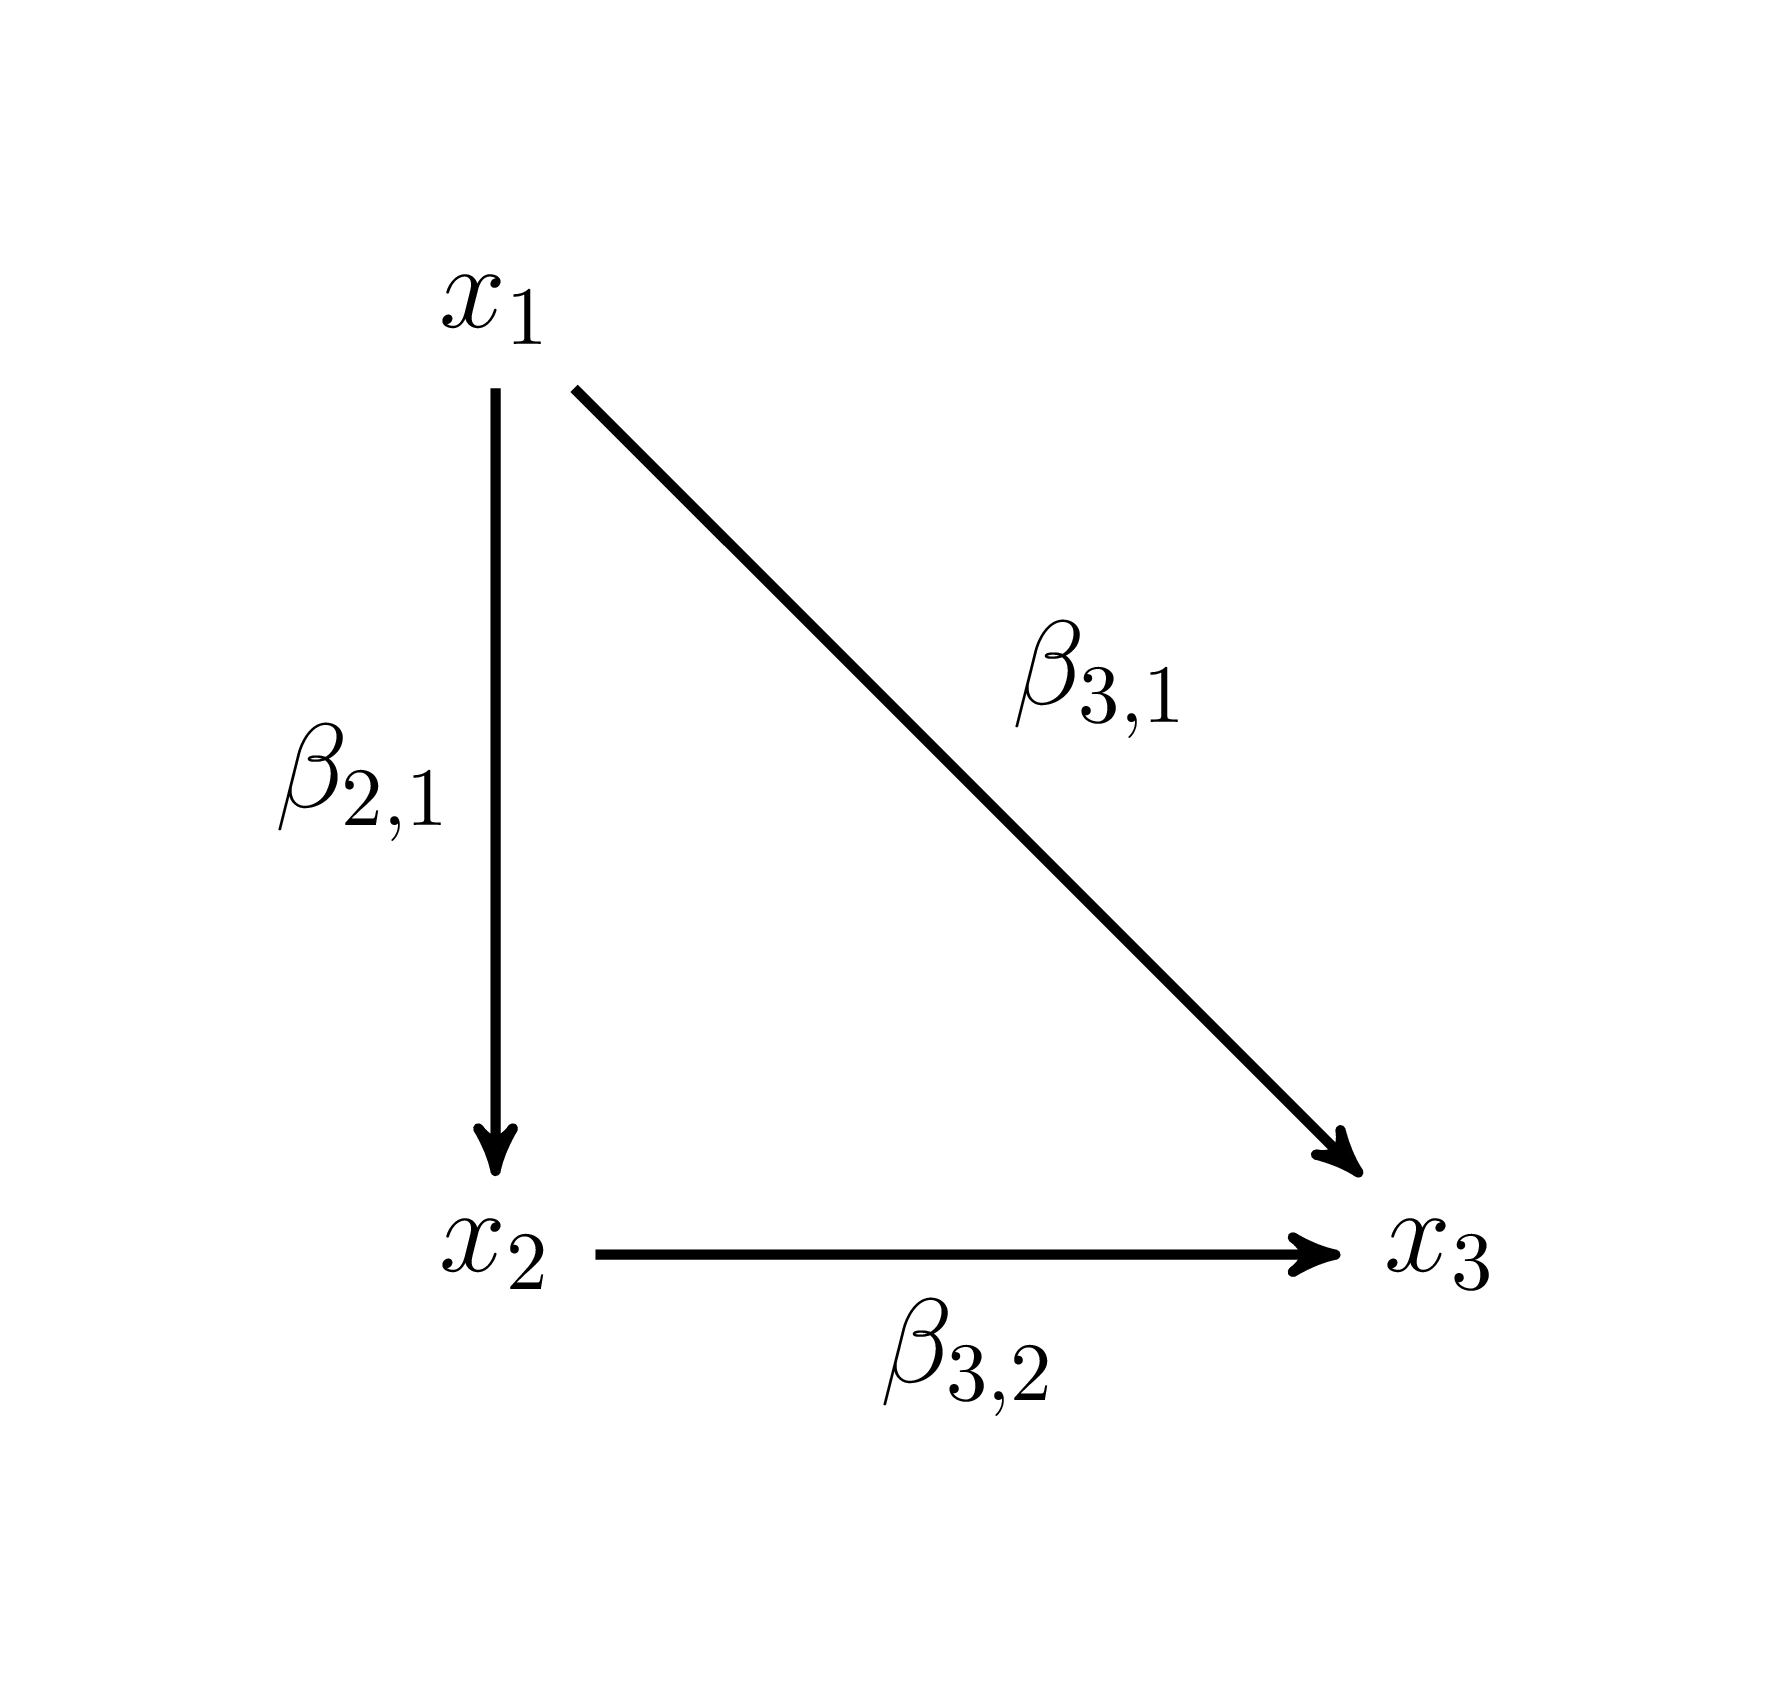
\includegraphics[width=0.5\linewidth,height=0.5\textheight]{image//mod3} 

}

\caption{Modèle à trois variables}\label{fig:mod3}
\end{figure}

La Figure \ref{fig:mod3} montre un modèle à trois variables. La première variable \(x_1\) prédit \(x_2\) et \(x_3\), en plus \(x_2\) prédit \(x_3\). Ce modèle peut aussi se représenter en matrice \(\mathbf{B}\) dans laquelle se retrouvent les coefficients de régression qui relient les variables. Dans ce cas-ci, \(\beta_{3,1}\) signifie que la variable 1 prédit la 3 à un degré \(\beta_{3,1}\); \(\beta_{3,2}\) signifie que la variable 2 prédit la 3 à un degré \(\beta_{3,2}\). Le premier indice correspond à l'effet (variable dépendante) et le deuxième à la cause (variable indépendante).

\begin{equation}
\mathbf{B} = 
\left( \begin{array}{ccc}
0 & 0 & 0 \\
\beta_{2,1} & 0 & 0 \\
\beta_{3,1} & \beta_{3,2} & 0 \\
\end{array} 
\right)
\label{eq:B}
\end{equation}

Afin de bâtir un exemple complet avec \textbf{R}, la syntaxe ci-dessous montre les paramètres arbitraires pour la création de données à parti du modèle de la figure \ref{fig:mod3}.

\begin{Shaded}
\begin{Highlighting}[]
\CommentTok{\# Pour reproductibilité}
\FunctionTok{set.seed}\NormalTok{(}\DecValTok{1448}\NormalTok{)            }
\NormalTok{n }\OtherTok{=} \DecValTok{100000}
\CommentTok{\# Paramètres arbitraire}
\NormalTok{beta21 }\OtherTok{=}\NormalTok{ .}\DecValTok{2} 
\NormalTok{beta31 }\OtherTok{=}\NormalTok{ .}\DecValTok{4}
\NormalTok{beta32 }\OtherTok{=} \SpecialCharTok{{-}}\NormalTok{.}\DecValTok{5}
\end{Highlighting}
\end{Shaded}

La première variable \(x_1\) est exogène, c'est-à-dire qu'elle n'est prédite par aucune autre variable, et n'obtient aucune information d'aucune autre variable. Cela paraît notamment dans la matrice \(\mathbf{B}\) avec la première ligne ne contenant que des 0. Ainsi, pour créer \texttt{x1}, il suffit de connaître sa variance (1 dans un scénario standardisé). Il faudra en supplément un vecteur de variances (ici, toutes fixées à 1 par le scénario standardisé).

\begin{Shaded}
\begin{Highlighting}[]
\CommentTok{\# Création de la première variable}
\NormalTok{x1 }\OtherTok{=} \FunctionTok{rnorm}\NormalTok{(}\AttributeTok{n =}\NormalTok{ n, }\AttributeTok{sd =} \DecValTok{1}\NormalTok{) }\CommentTok{\# Variance de 1}
\end{Highlighting}
\end{Shaded}

À l'aide de la loi de la somme des variances, la création de \(x_2\) est assez simple puisqu'il n'y a qu'un seul prédicteur.

\[
x_2 = \beta_{2,1}x_1+\epsilon_{x_2}
\]

En suivant l'équation \eqref{eq:eq29}, il est possible de calculer la variance résiduelle, toujours en assumant que \(\sigma^2_{x_1} = \sigma^2_{x_2}=1\).

\[
\sigma^2_{\epsilon_{x_2}} = 1-\beta_{2,1}^2\sigma^2_{x_1}=1-\beta_{21}^2
\]

En code \textbf{R}, il est possible de procéder ainsi.

\begin{Shaded}
\begin{Highlighting}[]
\CommentTok{\# Variance résiduelle}
\NormalTok{e\_x2 }\OtherTok{=} \DecValTok{1} \SpecialCharTok{{-}}\NormalTok{ beta21}\SpecialCharTok{\^{}}\DecValTok{2}

\CommentTok{\# Création de la variable}
\NormalTok{x2 }\OtherTok{=}\NormalTok{ beta21 }\SpecialCharTok{*}\NormalTok{ x1 }\SpecialCharTok{+} \FunctionTok{rnorm}\NormalTok{(}\AttributeTok{n =}\NormalTok{ n,  }\AttributeTok{sd =} \FunctionTok{sqrt}\NormalTok{(e\_x2)) }\CommentTok{\# Variance de 1}
\end{Highlighting}
\end{Shaded}

Maintenant, il reste à créer la variable \(x_3\). Celle-ci est générée à partir de \(x_1\) et \(x_2\) selon l'équation suivante.

\[
x_3 = \beta_{3,1}x_1 + \beta_{3,2}x_2 + \epsilon_{x_3}
\]

La variance résiduelle suit l'équation \eqref{eq:eq28}. En équation linéaire, elle s'écrit comme suit.

\[
\sigma^2{\epsilon_{x_3}} =\sigma^2_{x_3} -( \beta_{3,1}^2\sigma^2_{x_1} + \beta_{3,2}^2\sigma^2_{x_2}  +  2\beta_{3,1}\beta_{3,2}\sigma_{x_1,x_2}) = 1-(\beta_{3,1}^2+\beta_{3,2}^2  +  2\beta_{3,1}\beta_{3,2}\sigma_{x_1,x_2})
\]

Elle occasionne toutefois un défi, car la covariance entre \(x_1\) et \(x_2\) n'est pas explicitement connue. Dans le cas d'une variable prédite exclusivement par une autre variable qui elle est exogène (sans prédicteur), leur covariance est égale au coefficient de régression, soit \(\beta_{21}\). Ce cas ne survient que dans cette situation précise. Il sera impératif de dégager une solution générale pour des modèles ayant plus de trois variables, la complexité du calcul de la covariance augmentant avec la croissance de \(p\). En \textbf{R}, \(x_3\) se génère ainsi.

\begin{Shaded}
\begin{Highlighting}[]
\CommentTok{\# Variance résiduelle}
\NormalTok{e\_x3 }\OtherTok{=} \DecValTok{1} \SpecialCharTok{{-}}\NormalTok{ (beta31}\SpecialCharTok{\^{}}\DecValTok{2} \SpecialCharTok{+}\NormalTok{ beta32}\SpecialCharTok{\^{}}\DecValTok{2} \SpecialCharTok{+} \DecValTok{2} \SpecialCharTok{*}\NormalTok{ beta31 }\SpecialCharTok{*}\NormalTok{ beta32 }\SpecialCharTok{*}\NormalTok{ beta21)}

\CommentTok{\# Création de la variable}
\NormalTok{x3 }\OtherTok{=}\NormalTok{ beta31 }\SpecialCharTok{*}\NormalTok{ x1 }\SpecialCharTok{+}\NormalTok{ beta32 }\SpecialCharTok{*}\NormalTok{ x2 }\SpecialCharTok{+} \FunctionTok{rnorm}\NormalTok{(}\AttributeTok{n =}\NormalTok{ n,}
                                       \AttributeTok{sd =} \FunctionTok{sqrt}\NormalTok{(e\_x3)) }\CommentTok{\# Variance = 1}
\end{Highlighting}
\end{Shaded}

Il est possible de vérifier les caractéristiques des trois modèles soit

\begin{Shaded}
\begin{Highlighting}[]
\CommentTok{\# Création du jeu de données}
\NormalTok{X }\OtherTok{=} \FunctionTok{data.frame}\NormalTok{(}\AttributeTok{x1 =}\NormalTok{ x1,}
               \AttributeTok{x2 =}\NormalTok{ x2,}
               \AttributeTok{x3 =}\NormalTok{ x3)}

\CommentTok{\# Comme il s\textquotesingle{}agit d\textquotesingle{}un scénario standardisé, la matrice de}
\CommentTok{\# corrélation est similaire à la matrice de covariance.}
\FunctionTok{cov}\NormalTok{(X)}
\CommentTok{\#\textgreater{}       x1     x2     x3}
\CommentTok{\#\textgreater{} x1 1.002  0.202  0.303}
\CommentTok{\#\textgreater{} x2 0.202  1.004 {-}0.418}
\CommentTok{\#\textgreater{} x3 0.303 {-}0.418  0.997}
\FunctionTok{cor}\NormalTok{(X)}
\CommentTok{\#\textgreater{}       x1     x2     x3}
\CommentTok{\#\textgreater{} x1 1.000  0.201  0.303}
\CommentTok{\#\textgreater{} x2 0.201  1.000 {-}0.417}
\CommentTok{\#\textgreater{} x3 0.303 {-}0.417  1.000}

\CommentTok{\# Retrouver beta21}
\FunctionTok{lm}\NormalTok{(x2 }\SpecialCharTok{\textasciitilde{}}\NormalTok{ x1, }\AttributeTok{data =}\NormalTok{ X)}
\CommentTok{\#\textgreater{} }
\CommentTok{\#\textgreater{} Call:}
\CommentTok{\#\textgreater{} lm(formula = x2 \textasciitilde{} x1, data = X)}
\CommentTok{\#\textgreater{} }
\CommentTok{\#\textgreater{} Coefficients:}
\CommentTok{\#\textgreater{} (Intercept)           x1  }
\CommentTok{\#\textgreater{}     0.00148      0.20113}

\CommentTok{\# Retrouver beta31 et beta32}
\FunctionTok{lm}\NormalTok{(x3 }\SpecialCharTok{\textasciitilde{}}\NormalTok{ x1 }\SpecialCharTok{+}\NormalTok{ x2, }\AttributeTok{data =}\NormalTok{ X)}
\CommentTok{\#\textgreater{} }
\CommentTok{\#\textgreater{} Call:}
\CommentTok{\#\textgreater{} lm(formula = x3 \textasciitilde{} x1 + x2, data = X)}
\CommentTok{\#\textgreater{} }
\CommentTok{\#\textgreater{} Coefficients:}
\CommentTok{\#\textgreater{} (Intercept)           x1           x2  }
\CommentTok{\#\textgreater{}     0.00578      0.40254     {-}0.49663}
\end{Highlighting}
\end{Shaded}

Comme il s'agit d'un scénario standardisé, la matrice de corrélation est similaire à la matrice de covariance. Notamment, les variances sont près de \(1\). Aussi, les résultats confirment que la covariance entre \(x_1\) et \(x_2\) est bel et bien le coefficient de régression, mais surtout, comme il était mentionné, qu'il s'agit du seul cas où cela est vrai. Les régressions effectuées par \texttt{lm()} retrouvent également les \(\beta\) choisis pour l'exemple.

\hypertarget{cas-guxe9nuxe9ral}{%
\subsection{Cas général}\label{cas-guxe9nuxe9ral}}

Un cas général permet d'obtenir la matrice de covariance \(\mathbf{\Sigma}\) à partir de la matrice \(\mathbf{B}\) et d'un vecteur de variance \(\text{diag}(\mathbf{\Sigma})\). Par la suite, il est possible de créer des variables en série comme la section précédente, ou bien de revenir à ce qui se faisait dans les chapitres précédents, c'est-à-dire d'utiliser \texttt{MASS:mvrnorm()} pour générer des données.

Pour obtenir la matrice de covariance, il est nécessaire d'avoir une matrice de coefficients de régression

\begin{equation}
\mathbf{B} = 
\left( \begin{array}{cccc}
0 & 0 & 0 & 0\\
\beta_{2,1} & 0 & 0 & 0\\
...& ...  & 0 & 0 \\
\beta_{p,1} & ... & \beta_{p,p-1} & 0
\end{array} 
\right)
\label{eq:B2}
\end{equation}

et d'un vecteur de variances

\begin{equation}
\text{diag}(\mathbf{\Sigma}) = \left(\sigma^2_{x_1},...,\sigma^2_{x_p} \right)
\end{equation}

Ces matrices sont construites de façon générale. La matrice \(\mathbf{B}\) est de dimension \(p \times p\) avec des valeurs nulles comme triangle supérieur incluant la diagonale et toutes celles qui se trouvent au-dessus. Les coefficients de régresison se trouvent dans le triangle extérieur. Le vecteur de variance contient \(p\) valeurs qui représentent les variances de variables. Elles sont toutes à l'unité quand le scénario est standardisé.

L'idée sous-jacente est qu'il est possible de calculer les covariances de la variable \(i\) à partir de la matrice de covariance des variables précédente \(1:(i-1)\) soit \(\mathbf{\Sigma}_{1:(i-1),1:(i-1)}\) et des coefficients de régression associés \(\mathbf{B}_{i, 1:(i-1)}\) en procédant en série pour toutes variables de \(x_2\) (\(i=2\)) (prédite par au moins une variable, toutes sauf la première) jusqu'à la dernière variable \(x_p\) (\(i=p\)). Le calcul est décrit à l'équation \eqref{eq:buildS}, malheureusement, elle recourt à l'algèbre matricielle, mais demeure toujours beaucoup plus simple et générale que si elle était présentée en algèbre linéaire.

\begin{equation}
\begin{aligned}
\mathbf{\Sigma}_{i,1:(i-1)} = \mathbf{B}_{i+1,1:i}\mathbf{\Sigma}_{1:i,1:i}\\
\mathbf{\Sigma}_{1:(i-1),i} = \mathbf{B}_{i+1,1:i}\mathbf{\Sigma}_{1:i,1:i}
\end{aligned}
\label{eq:buildS}
\end{equation}

Il faut à chaque étape s'assurer de faire le remplacement des valeurs obtenues sur chaque côté de la diagonale, ce pourquoi deux équations sont reproduites à l'équaiton \eqref{eq:buildS} avec des indices différents pour \(\mathbf{\Sigma}\).

\begin{Shaded}
\begin{Highlighting}[]
\CommentTok{\# Matrice B}
\NormalTok{B }\OtherTok{=} \FunctionTok{matrix}\NormalTok{(}\FunctionTok{c}\NormalTok{(   }\DecValTok{0}\NormalTok{,     }\DecValTok{0}\NormalTok{,    }\DecValTok{0}\NormalTok{,}
\NormalTok{             beta21,   }\DecValTok{0}\NormalTok{,    }\DecValTok{0}\NormalTok{,}
\NormalTok{             beta31, beta32, }\DecValTok{0}\NormalTok{), }
           \AttributeTok{ncol  =} \DecValTok{3}\NormalTok{, }\AttributeTok{nrow =} \DecValTok{3}\NormalTok{, }\AttributeTok{byrow =} \ConstantTok{TRUE}\NormalTok{)}

\CommentTok{\# Vecteur de variances}
\NormalTok{V }\OtherTok{=} \FunctionTok{c}\NormalTok{(}\DecValTok{1}\NormalTok{, }\DecValTok{1}\NormalTok{, }\DecValTok{1}\NormalTok{)}

\CommentTok{\# Montrer}
\NormalTok{B}
\CommentTok{\#\textgreater{}      [,1] [,2] [,3]}
\CommentTok{\#\textgreater{} [1,]  0.0  0.0    0}
\CommentTok{\#\textgreater{} [2,]  0.2  0.0    0}
\CommentTok{\#\textgreater{} [3,]  0.4 {-}0.5    0}
\end{Highlighting}
\end{Shaded}

Voici pour l'exemple précédent les étapes de calcul décrites une à une de l'équation \eqref{eq:buildS}. D'abord, il faut construire une matrice, \(\mathbf{\Sigma}\) (\texttt{S} en code \textbf{R} ci-dessous) avec comme diagonale les variances. Puis, calculer l'équation \eqref{eq:buildS}. Ensuite, il faut remplacer le résultat obtenu des deux côtés de la diagonale de façon à ce que \texttt{S} demeure symétrique. Ces étapes sont répétées pour \(i=2,...,p\) (dans cet exemple, \(p=3\)).

\begin{Shaded}
\begin{Highlighting}[]
\CommentTok{\# Créer une matrice de covariance préliminaire}
\NormalTok{S }\OtherTok{=} \FunctionTok{diag}\NormalTok{(V)}

\CommentTok{\# Aucune covariance n\textquotesingle{}est inscrite dans S}
\NormalTok{S}
\CommentTok{\#\textgreater{}      [,1] [,2] [,3]}
\CommentTok{\#\textgreater{} [1,]    1    0    0}
\CommentTok{\#\textgreater{} [2,]    0    1    0}
\CommentTok{\#\textgreater{} [3,]    0    0    1}

\CommentTok{\# Première variable}
\NormalTok{i }\OtherTok{=} \DecValTok{2}

\CommentTok{\# Calcul de la covariance entre x1 et x2}
\NormalTok{B[i, }\DecValTok{1}\SpecialCharTok{:}\NormalTok{(i}\DecValTok{{-}1}\NormalTok{)] }\SpecialCharTok{\%*\%}\NormalTok{ S[}\DecValTok{1}\SpecialCharTok{:}\NormalTok{(i}\DecValTok{{-}1}\NormalTok{),}\DecValTok{1}\SpecialCharTok{:}\NormalTok{(i}\DecValTok{{-}1}\NormalTok{)]}
\CommentTok{\#\textgreater{}      [,1]}
\CommentTok{\#\textgreater{} [1,]  0.2}

\CommentTok{\# Il faut remplacer ce résultat de chaque côté de la diagonale}
\CommentTok{\# Calcul de la covariance entre x1 et x2 assignée à COV}
\NormalTok{COV }\OtherTok{=}\NormalTok{ B[i, }\DecValTok{1}\SpecialCharTok{:}\NormalTok{(i}\DecValTok{{-}1}\NormalTok{)] }\SpecialCharTok{\%*\%}\NormalTok{ S[}\DecValTok{1}\SpecialCharTok{:}\NormalTok{(i}\DecValTok{{-}1}\NormalTok{),}\DecValTok{1}\SpecialCharTok{:}\NormalTok{(i}\DecValTok{{-}1}\NormalTok{)]}
\NormalTok{S[i, }\DecValTok{1}\SpecialCharTok{:}\NormalTok{(i}\DecValTok{{-}1}\NormalTok{)] }\OtherTok{=}\NormalTok{ COV}
\NormalTok{S[}\DecValTok{1}\SpecialCharTok{:}\NormalTok{(i}\DecValTok{{-}1}\NormalTok{),i] }\OtherTok{=}\NormalTok{ COV}

\CommentTok{\# La matrice est mise à jour pour i = 2}
\NormalTok{S}
\CommentTok{\#\textgreater{}      [,1] [,2] [,3]}
\CommentTok{\#\textgreater{} [1,]  1.0  0.2    0}
\CommentTok{\#\textgreater{} [2,]  0.2  1.0    0}
\CommentTok{\#\textgreater{} [3,]  0.0  0.0    1}

\CommentTok{\# Pour i = 3, l\textquotesingle{}équation est reprise}
\NormalTok{i }\OtherTok{=} \DecValTok{3}
\CommentTok{\# Calcul de la covariance entre x1 et x2 assignée à COV}
\NormalTok{COV }\OtherTok{=}\NormalTok{ B[i, }\DecValTok{1}\SpecialCharTok{:}\NormalTok{(i}\DecValTok{{-}1}\NormalTok{)] }\SpecialCharTok{\%*\%}\NormalTok{ S[}\DecValTok{1}\SpecialCharTok{:}\NormalTok{(i}\DecValTok{{-}1}\NormalTok{), }\DecValTok{1}\SpecialCharTok{:}\NormalTok{(i}\DecValTok{{-}1}\NormalTok{)]}
\NormalTok{S[i, }\DecValTok{1}\SpecialCharTok{:}\NormalTok{(i}\DecValTok{{-}1}\NormalTok{)] }\OtherTok{=}\NormalTok{ COV}
\NormalTok{S[}\DecValTok{1}\SpecialCharTok{:}\NormalTok{(i}\DecValTok{{-}1}\NormalTok{), i] }\OtherTok{=}\NormalTok{ COV}

\CommentTok{\# La matrice est mise à jour pour i = 3}
\NormalTok{S}
\CommentTok{\#\textgreater{}      [,1]  [,2]  [,3]}
\CommentTok{\#\textgreater{} [1,]  1.0  0.20  0.30}
\CommentTok{\#\textgreater{} [2,]  0.2  1.00 {-}0.42}
\CommentTok{\#\textgreater{} [3,]  0.3 {-}0.42  1.00}

\CommentTok{\# Elle est approximativement identique aux données de l\textquotesingle{}exemple précédent}
\FunctionTok{cov}\NormalTok{(X)}
\CommentTok{\#\textgreater{}       x1     x2     x3}
\CommentTok{\#\textgreater{} x1 1.002  0.202  0.303}
\CommentTok{\#\textgreater{} x2 0.202  1.004 {-}0.418}
\CommentTok{\#\textgreater{} x3 0.303 {-}0.418  0.997}
\end{Highlighting}
\end{Shaded}

Avant de procéder, une courte digression sur une façon de réaliser en moins de lignes, mais avec une syntaxe plus complexe, la réassignation des valeurs dans \texttt{S}. Le code est présenté dans la syntaxe ci-dessous. Il appert qu'il n'est pas aussi intéressant à programmer pour sauver deux lignes.

\begin{Shaded}
\begin{Highlighting}[]
\CommentTok{\# Une note pour indiquer que les valeurs à remplacer pourrait}
\CommentTok{\# être fait en une seule ligne de syntaxe en bénéficiant du }
\CommentTok{\# recycle vectoriel de R, mais la solution n\textquotesingle{}est ni simple, ni élégante.}
\NormalTok{remplacer }\OtherTok{=} \FunctionTok{cbind}\NormalTok{(}\FunctionTok{c}\NormalTok{(}\FunctionTok{rep}\NormalTok{(i, i}\DecValTok{{-}1}\NormalTok{), }\DecValTok{1}\SpecialCharTok{:}\NormalTok{(i}\DecValTok{{-}1}\NormalTok{)), }\FunctionTok{c}\NormalTok{(}\DecValTok{1}\SpecialCharTok{:}\NormalTok{(i}\DecValTok{{-}1}\NormalTok{), }\FunctionTok{rep}\NormalTok{(i, i}\DecValTok{{-}1}\NormalTok{)))}
\NormalTok{S[remplacer]}
\end{Highlighting}
\end{Shaded}

Trêve de digression, une fois la matrice de covariance \texttt{S} calculée, la fonction \texttt{MASS::mvrnorm()} peut être utilisée pour créer des données. Les résultats sont presque identiques pour les régressions.

\begin{Shaded}
\begin{Highlighting}[]
\FunctionTok{set.seed}\NormalTok{(}\DecValTok{1448}\NormalTok{) }\CommentTok{\# La même que l\textquotesingle{}exemple précédent}

\CommentTok{\# Création de données}
\NormalTok{X }\OtherTok{=}\NormalTok{ MASS}\SpecialCharTok{::}\FunctionTok{mvrnorm}\NormalTok{(}\AttributeTok{n =}\NormalTok{ n, }\AttributeTok{mu =} \FunctionTok{c}\NormalTok{(}\DecValTok{0}\NormalTok{, }\DecValTok{0}\NormalTok{, }\DecValTok{0}\NormalTok{), }\AttributeTok{Sigma =}\NormalTok{ S)}

\CommentTok{\# Configurer en tableau de données (data.frame)}
\NormalTok{X }\OtherTok{=} \FunctionTok{as.data.frame}\NormalTok{(X)}
\FunctionTok{colnames}\NormalTok{(X) }\OtherTok{=} \FunctionTok{c}\NormalTok{(}\StringTok{"x1"}\NormalTok{,}\StringTok{"x2"}\NormalTok{,}\StringTok{"x3"}\NormalTok{)}

\CommentTok{\# Retrouver beta21}
\FunctionTok{lm}\NormalTok{(x2 }\SpecialCharTok{\textasciitilde{}}\NormalTok{ x1, }\AttributeTok{data =}\NormalTok{ X)}
\CommentTok{\#\textgreater{} }
\CommentTok{\#\textgreater{} Call:}
\CommentTok{\#\textgreater{} lm(formula = x2 \textasciitilde{} x1, data = X)}
\CommentTok{\#\textgreater{} }
\CommentTok{\#\textgreater{} Coefficients:}
\CommentTok{\#\textgreater{} (Intercept)           x1  }
\CommentTok{\#\textgreater{}    {-}0.00219      0.20191}

\CommentTok{\# Retrouver beta31 et beta32}
\FunctionTok{lm}\NormalTok{(x3 }\SpecialCharTok{\textasciitilde{}}\NormalTok{ x1 }\SpecialCharTok{+}\NormalTok{ x2, }\AttributeTok{data =}\NormalTok{ X)}
\CommentTok{\#\textgreater{} }
\CommentTok{\#\textgreater{} Call:}
\CommentTok{\#\textgreater{} lm(formula = x3 \textasciitilde{} x1 + x2, data = X)}
\CommentTok{\#\textgreater{} }
\CommentTok{\#\textgreater{} Coefficients:}
\CommentTok{\#\textgreater{} (Intercept)           x1           x2  }
\CommentTok{\#\textgreater{}    {-}0.00579      0.40295     {-}0.49899}
\end{Highlighting}
\end{Shaded}

Comme la formule est générale et qu'elle implique plusieurs itérations, il est envisageable de programmer ces calculs avec une boucle dans une fonction maison. La fonction maison \texttt{beta2cov()} permet à partir d'une matrice de coefficient de régression et de

\begin{Shaded}
\begin{Highlighting}[]
\CommentTok{\# De Beta vers covariance (beta 2 covariance)}
\NormalTok{beta2cov }\OtherTok{=} \ControlFlowTok{function}\NormalTok{(B, }\AttributeTok{V =} \ConstantTok{NULL}\NormalTok{)\{}
  
\NormalTok{  p }\OtherTok{=} \FunctionTok{dim}\NormalTok{(B)[}\DecValTok{1}\NormalTok{]                 }\CommentTok{\# Nombre de variables}
  
  \ControlFlowTok{if}\NormalTok{(}\FunctionTok{is.null}\NormalTok{(V))\{               }\CommentTok{\# Si V est nulle, alors V est une}
\NormalTok{    S }\OtherTok{=} \FunctionTok{diag}\NormalTok{(p)                 }\CommentTok{\# matrice diagonale d\textquotesingle{}identité,}
\NormalTok{  \}}\ControlFlowTok{else}\NormalTok{\{                        }\CommentTok{\# autrement il s\textquotesingle{}agit d\textquotesingle{}une matrice}
\NormalTok{    S }\OtherTok{=} \FunctionTok{diag}\NormalTok{(V)                 }\CommentTok{\# avec les variances en diagonale}
\NormalTok{  \}  }
  
  \CommentTok{\# Boucle de calcul pour la covariance de la variable i (i = 2:p)}
  \ControlFlowTok{for}\NormalTok{(i }\ControlFlowTok{in} \DecValTok{2}\SpecialCharTok{:}\NormalTok{p)\{}
\NormalTok{    COV }\OtherTok{=}\NormalTok{ B[(i), (}\DecValTok{1}\SpecialCharTok{:}\NormalTok{(i}\DecValTok{{-}1}\NormalTok{))] }\SpecialCharTok{\%*\%}\NormalTok{ S[}\DecValTok{1}\SpecialCharTok{:}\NormalTok{(i}\DecValTok{{-}1}\NormalTok{), }\DecValTok{1}\SpecialCharTok{:}\NormalTok{(i}\DecValTok{{-}1}\NormalTok{)]}
\NormalTok{    S[i, }\DecValTok{1}\SpecialCharTok{:}\NormalTok{(i}\DecValTok{{-}1}\NormalTok{)] }\OtherTok{=}\NormalTok{ COV}
\NormalTok{    S[}\DecValTok{1}\SpecialCharTok{:}\NormalTok{(i}\DecValTok{{-}1}\NormalTok{), i] }\OtherTok{=}\NormalTok{ COV}
\NormalTok{  \}}
  
  \FunctionTok{return}\NormalTok{(S)}
  
\NormalTok{\}}
\end{Highlighting}
\end{Shaded}

Évidemment, comme il est possible de passer de matrice de coefficient de régression à une matrice de covariance, il est possible de faire l'inverse. L'équation \eqref{eq:buildS} est réarrangée pour isoler \(\mathbf{B}\) de l'équation ce qui donne l'équation \eqref{eq:buildB}.

\begin{equation}
\mathbf{B}_{i+1, 1:i} = \mathbf{\Sigma}^{-1}_{1:i,1:i}\mathbf{\Sigma}_{1+i,1:i}
\label{eq:buildB}
\end{equation}

L'équation \eqref{eq:buildB} se transforme (relativement) aisément en fonction maison. Par rapport à \texttt{beta2cov()}, la boucle n'inclut pas la \(p\)\textsuperscript{e} variable, mais bien la première.

\begin{Shaded}
\begin{Highlighting}[]
\CommentTok{\# De la covariance à Beta (cov2beta)}
\NormalTok{cov2beta }\OtherTok{=} \ControlFlowTok{function}\NormalTok{(S)\{}
  
\NormalTok{  p }\OtherTok{=} \FunctionTok{dim}\NormalTok{(S)[}\DecValTok{1}\NormalTok{]          }\CommentTok{\# Nombre de variable}
\NormalTok{  BETA }\OtherTok{=} \FunctionTok{matrix}\NormalTok{(}\DecValTok{0}\NormalTok{, p, p) }\CommentTok{\# Matrice vide}
  
  \CommentTok{\# Boucle de calcul pour la covariance de la variable i (i = 1:(p{-}1))}
  \ControlFlowTok{for}\NormalTok{(i }\ControlFlowTok{in} \DecValTok{1}\SpecialCharTok{:}\NormalTok{(p}\DecValTok{{-}1}\NormalTok{))\{}
\NormalTok{    BETA[i}\SpecialCharTok{+}\DecValTok{1}\NormalTok{, }\DecValTok{1}\SpecialCharTok{:}\NormalTok{i] }\OtherTok{=} \FunctionTok{solve}\NormalTok{(S[}\DecValTok{1}\SpecialCharTok{:}\NormalTok{i, }\DecValTok{1}\SpecialCharTok{:}\NormalTok{i], S[}\DecValTok{1}\SpecialCharTok{+}\NormalTok{i, }\DecValTok{1}\SpecialCharTok{:}\NormalTok{i])}
\NormalTok{  \}}
  
  \FunctionTok{return}\NormalTok{(BETA)}
  
\NormalTok{\}}
\end{Highlighting}
\end{Shaded}

La fonction maison \texttt{cov2beta()} est maintenant testée sur \texttt{S} pour évaluer si elle retourne bien la matrice \texttt{B} originale.

\begin{Shaded}
\begin{Highlighting}[]
\FunctionTok{cov2beta}\NormalTok{(S)}
\CommentTok{\#\textgreater{}      [,1] [,2] [,3]}
\CommentTok{\#\textgreater{} [1,]  0.0  0.0    0}
\CommentTok{\#\textgreater{} [2,]  0.2  0.0    0}
\CommentTok{\#\textgreater{} [3,]  0.4 {-}0.5    0}
\end{Highlighting}
\end{Shaded}

Ce qui est le cas.

Une seule contrainte s'impose lors de la du calcul de la covariance à partir des coefficients de régression. Il s'agit de s'assurer que la matrice de covariance demeure positive semi-définie à chaque étape. Cela se manifeste notamment lorsque les coefficients de régression pour une variable dépendante sont si élevés que le coefficient de détermination surpasse la variance de la variable en question. Autrement dit, la variance de la variable n'est pas assez élevée pour le potentiel explicatif. Mathématiquement le problème est que \(1-R^2_X < 0\) ou plus généralement que \(\sigma^2_y-\mathbf{B^\prime\Sigma B}<0\). Dans ces cas, la variance résiduelle négative, ce qui est impossible. L'une des corrections a apporté sont les suivantes, réduire les coefficients de régression \(\mathbf{B}\) pour cette variable ou encore d'augmenter sa variance \(\sigma^2_y\) de sorte que \(\sigma^2_y-\mathbf{B^\prime\Sigma B}>=0\) soit toujours vrai à chaque étape.

Une dernière note, comme ces équations et syntaxes procèdent de \(i=2,...,p\), l'ordre des variables est primordiale et interchanger leur ordre a des conséquences substantielles sur les résultats. Lorsque la matrice \(\mathbf{B}\) est créées, il faut être sûr de l'ordre \emph{déterministe} des variables, c'est-à-dire, quelle variable \emph{cause} quelles autres variables, comme c'était spécifié à la Figure \ref{fig:mod3} par exemple. Changer ou retirer ne serait-ce qu'une variable changerait les coefficients de régression : les régressions ne seraient plus identiques, la matrice de coefficients de régression ne serait pas retrouvée. Il ne faut pas être surpris donc, si les résultats changent dans cette situation. Nonobstant, changer ou retirer une variable peut être pertinent dans certains contextes, surtout pour l'étude de la \textbf{misspécification} (en anglais) des modèles, c'est-à-dire lorsqu'un modèle erroné est utilisé plutôt que le vrai modèle, ce qui entraîne notamment des biais. Les études à ce sujet emprunteront une méthode statistique similaire.

\hypertarget{simulations}{%
\chapter{Simulations}\label{simulations}}

Dans plusieurs contextes statistiques, les informations cruciales nécessaires pour réaliser une analyse statistique ou tirer des résultats spécifiques ne sont pas connues. Pire, parfois certains postulats sont violés rendant les démarches usuelles caduques. Enfin, dans certains contextes, une analyse formelle pourrait s'avérer fort complexe, voire irrésoluble, alors qu'une analyse plus empirique usant des techniques de rééchantillonnage résoudra ces problèmes simplement et immédiatement.

Jusqu'à présent, les situations connues des analyses statistiques ont été présentées. Maintenant, les techniques de rééchantillonnage, comme le bootstrap et de simulations Monte-Carlo seront présentés.

\hypertarget{les-simulations-monte-carlo}{%
\section{Les simulations Monte-Carlo}\label{les-simulations-monte-carlo}}

Les simulations Monte-Carlo sont une famille de méthode algorithmique qui permet de calculer une valeur numérique en utilisant des procédés aléatoires. Le nom provient du prestigieux casino de Monte-Carlo à Monaco sur la Côte d'Azur, où des jeux de hasard se jouent constamment, et ayant ainsi une connotation très forte avec le hasard et les nombres aléatoires.

Une simulation de Monte-Carlo prédit une étendue de résultats possibles à partir d'un ensemble de valeurs d'entrée fixes et en tenant compte de l'incertitude inhérente de certaines variables. En d'autres termes, une simulation de Monte-Carlo produit les résultats possibles (sorties) d'un modèle à partir des entrées fixes et d'autres entrées variables. Ces sorties sont calculées encore et encore (des milliers de fois, parfois plus), en utilisant à chaque fois un ensemble différent de nombres aléatoires, générant des sorties probables, mais différentes à chaque fois. Les estimations (et leur tendance) obtenues peuvent alors être interprétées.

Les simulations Monte-Carlo sont particulièrement utiles, car elles permettent, en mathématiques, de calculer des intégrales très complexes; en physique, d'estimer la forme d'un signal ou la sensibilité; en finance, simulent des conditions permettant de prévoir le marché; et en psychologie, simuler des processus comportementaux ou cognitifs.

Les simulations Monte-Carlo possèdent trois caractéristiques ou étapes :

\begin{enumerate}
\def\labelenumi{\arabic{enumi}.}
\item
  Construire un modèle ayant des variables indépendantes (entrées) et dépendantes (sorties);
\item
  Spécifier les caractéristiques aléatoires des variables indépendantes et définir des valeurs crédibles;
\item
  Rouler les simulations de façon répétitive jusqu'à ce que suffisamment d'itérations soient produites et que les résultats convergent vers une solution.
\end{enumerate}

Maintenant, ces étapes sont mises en contexte avec un problème.

\hypertarget{le-probluxe8me-de-monty-hall}{%
\subsection{Le problème de Monty-Hall}\label{le-probluxe8me-de-monty-hall}}

Rien de mieux pour confronter le sens commun que d'être confronté à un problème contre-intuitif. Les simulations Monte-Carlo nous permettront de vérifier les résultats de façon empirique, parallèlement à ce qu'une analyse formelle fournit.

Le problème de Monty Hall \autocite[attribuables à][]{Selvin75} présente un joueur devant un présentateur (Monty Hall). Trois portes sont offertes au choix du joueur. Derrière l'une d'entre elles se retrouve un magnifique prix : une voiture \emph{électrique} de luxe. Derrière chacune des deux autres portes se retrouvent un prix citron : une chèvre chacune. Le joueur ne sait pas ce qu'il y derrière les portes. Le joueur peut alors choisir une porte. Évidemment, à ce moment le joueur à une chance sur trois de choisir la voiture.

\begin{figure}
\centering
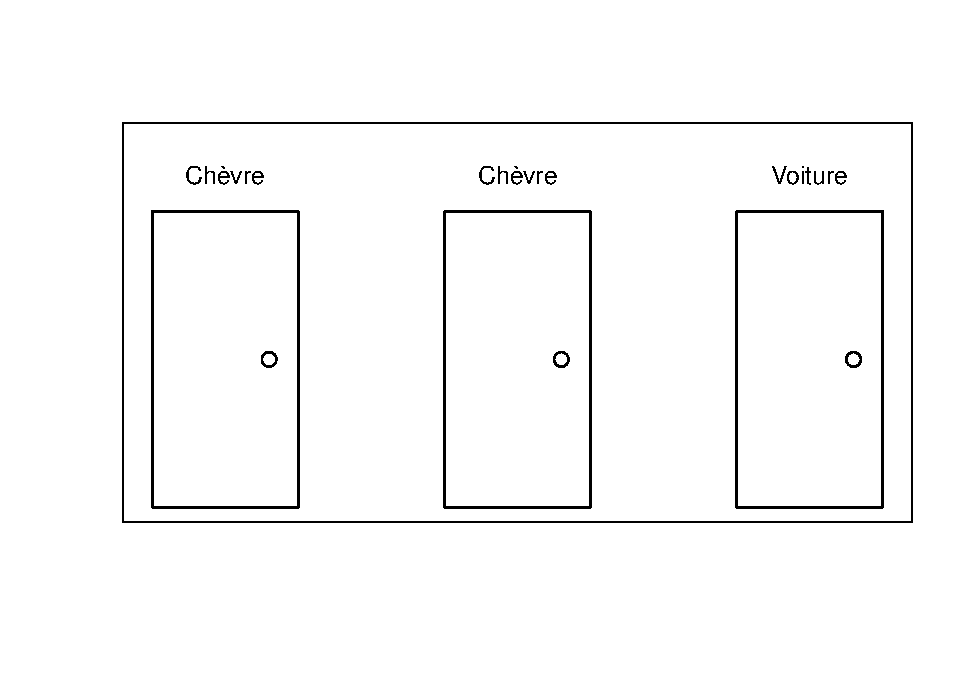
\includegraphics{06-Simuler_files/figure-latex/MH-1.pdf}
\caption{\label{fig:MH}Illustration du problème de Monty Hall}
\end{figure}

Par la suite, le présentateur, qui connaît le contenu derrière les portes, ouvre une porte qui (a) ne cache pas la voiture et (b) que le participant n'a pas choisie. Le joueur peut alors choisir (a) de conserver la porte choisie ou (b) de changer de porte. Quelle option, s'il y en a une, assurera le meilleur gain (choisir la voiture)? Rester ou changer? Par exemple, suivant l'illustration de la figure \ref{fig:MH}, le joueur choisit la porte 1, alors le présentateur doit ouvrir la porte 2 (non choisie et ne contient pas la voiture). Le joueur doit-il changer son choix? Ici, la réponse est évidente, car la réponse est connue. Qu'en est-il alors si le joueur avait choisi la porte 3 et le présentateur ouvert l'une des deux autres porte? \emph{Le joueur doit-il changer ou rester?} La question sous-jacente est qu'elles sont les probabilités de rester et changer respectivement. Sont-elles différentes?

Comme le résultat n'est pas des plus intuitif (et sans divulgâcher le résultat), une petite simulation s'impose (ou une analyse formelle pour les lecteurs enclins mathématiquement). La situation sera recréée un millier de fois pour vérifier l'option (rester ou changer) qui maximise de gagner la voiture.

En se référant aux trois points caractérisant une simulation Monte-Carlo susmentionné :

\begin{enumerate}
\def\labelenumi{\arabic{enumi}.}
\item
  Le problème de Monty Hall tel qu'imminemment décrit.
\item
  Les variables indépendantes sont (a) le tirage aléatoire du contenu derrière les portes (distribution uniforme, chaque porte à la même probabilité d'avoir un prix ou non), (b) le choix du joueur (distribution uniforme, pourrait être différent), et (c) la porte ouverte par le présentateur. Deux variables indépendantes sont fixes (les deux options sont étudiées), l'action de rester ou de changer. Il y a deux variables dépendantes, le succès (choisir le prix) ou l'échec (choisir une autre porte) de rester ou de changer.
\item
  La simulation est reprise 1000 fois.
\end{enumerate}

La simulation doit comporter une distribution aléatoire du contenu derrière les trois portes, identifier une porte gagnante et deux perdantes. Il est intéressant de note que, sur le plan de computationnelle, il est inutile d'attribuer aléatoirement la porte gagnante, toutefois le scénario sera plus acceptable pour un lecteur scrupuleux. Par la suite, le joueur fait son premier choix. Ici, plusieurs modèles peuvent être utilisés, comme constamment choisir la même porte (ce qui simplifie la situation et ne change pas les probabilités parce que le contenu des portes, lui, est aléatoire) ou, pour rester vrai à la situation, le joueur fera un choix aléatoire. Le comportement du présentateur s'enclenche, il doit ``ouvrir'' une porte non choisie et qui ne contient pas le prix. Les deux stratégies sont alors étudiées, rester versus changer. La simulation enregistre alors s'il y a eu gain ou non et l'additionne au total de chacun. La simulation est reprise un nombre important de fois, ici, 1000 suffira, mais des situations compliquées peuvent demander beaucoup plus d'itérations.

\begin{Shaded}
\begin{Highlighting}[]
\CommentTok{\# Simulation du problème de Monty Hall}
\NormalTok{portes }\OtherTok{=} \FunctionTok{c}\NormalTok{(}\StringTok{"Chèvre"}\NormalTok{,}\StringTok{"Chèvre"}\NormalTok{,}\StringTok{"Voiture"}\NormalTok{)}
\NormalTok{reps }\OtherTok{=} \DecValTok{1000}
\FunctionTok{set.seed}\NormalTok{(}\DecValTok{7896}\NormalTok{)}
\CommentTok{\# Valeur initial des gains}
\NormalTok{gain.rester }\OtherTok{=} \DecValTok{0}
\NormalTok{gain.changer }\OtherTok{=} \DecValTok{0}

\ControlFlowTok{for}\NormalTok{(i }\ControlFlowTok{in} \DecValTok{1}\SpecialCharTok{:}\NormalTok{reps)\{}
  \CommentTok{\# Arrangement initial des portes}
\NormalTok{  tirage }\OtherTok{=} \FunctionTok{sample}\NormalTok{(portes)}
  \CommentTok{\# Trouver le prix}
\NormalTok{  prix }\OtherTok{=} \FunctionTok{which}\NormalTok{(tirage }\SpecialCharTok{\%in\%} \StringTok{"Voiture"}\NormalTok{)}
  \CommentTok{\# Choix aléatoire}
\NormalTok{  choix1 }\OtherTok{=} \FunctionTok{sample}\NormalTok{(}\FunctionTok{length}\NormalTok{(portes), }\AttributeTok{size =} \DecValTok{1}\NormalTok{)}

  \CommentTok{\# Sélectionner la porte avec la chèvre (pas un prix) et}
  \CommentTok{\# qui n\textquotesingle{}est pas celle choisie (choix1)}
\NormalTok{  option }\OtherTok{=} \FunctionTok{c}\NormalTok{(choix1, prix)}
  \ControlFlowTok{if}\NormalTok{(choix1 }\SpecialCharTok{!=}\NormalTok{ prix)\{}
    \CommentTok{\# Si une porte valide}
\NormalTok{    monty }\OtherTok{=} \FunctionTok{c}\NormalTok{(}\DecValTok{1}\SpecialCharTok{:}\DecValTok{3}\NormalTok{)[}\SpecialCharTok{{-}}\NormalTok{option]}
\NormalTok{  \}}\ControlFlowTok{else}\NormalTok{\{}
    \CommentTok{\# Si deux portes valides, en choisir une aléatoirement.}
\NormalTok{    monty }\OtherTok{=} \FunctionTok{sample}\NormalTok{(}\FunctionTok{c}\NormalTok{(}\DecValTok{1}\SpecialCharTok{:}\DecValTok{3}\NormalTok{)[}\SpecialCharTok{{-}}\NormalTok{option], }\AttributeTok{size =} \DecValTok{1}\NormalTok{)}
\NormalTok{  \}}
  \CommentTok{\# Décision : Reste à choix1}
\NormalTok{  choix.rester }\OtherTok{=}\NormalTok{ choix1}

  \CommentTok{\# Décision : Changer de choix changer}
  \CommentTok{\# Changer = ne pas prendre la porte initial, ni la porte ouverte}
\NormalTok{  choix.changer }\OtherTok{=} \FunctionTok{c}\NormalTok{(}\DecValTok{1}\SpecialCharTok{:}\DecValTok{3}\NormalTok{)[}\SpecialCharTok{{-}}\FunctionTok{c}\NormalTok{(choix1, monty)]}

  \CommentTok{\# Enregistrement des gains}
\NormalTok{  gain.rester }\OtherTok{=}\NormalTok{ gain.rester }\SpecialCharTok{+}\NormalTok{ (tirage[choix.rester] }\SpecialCharTok{==} \StringTok{"Voiture"}\NormalTok{)}
\NormalTok{  gain.changer }\OtherTok{=}\NormalTok{ gain.changer }\SpecialCharTok{+}\NormalTok{ (tirage[choix.changer] }\SpecialCharTok{==} \StringTok{"Voiture"}\NormalTok{)}
\NormalTok{\}}

\FunctionTok{cbind}\NormalTok{(gain.rester,gain.changer)  }\SpecialCharTok{/}\NormalTok{ reps}
\CommentTok{\#\textgreater{}      gain.rester gain.changer}
\CommentTok{\#\textgreater{} [1,]       0.316        0.684}
\end{Highlighting}
\end{Shaded}

Une petite digression avant de poursuivre. À cause d'un inconvénient de la fonction \texttt{sample()}, une approche conditionnelle est utilisée. En fait, la fonction échantillonne les éléments de \texttt{x} (premier argument) jusqu'à obtenir \texttt{size} objets. Par contre, si une seule valeur est donnée à \texttt{x} et si elle est numérique, alors la fonction utilise les éléments de \texttt{1:x} pour rééchantillonner. Ici, si le choix et le prix sont différents, il n'y a qu'une seule valeur retournée (l'autre chèvre), ce qui occasionne le problème, et par conséquent, de l'utilisation du conditionnel. En programmation, il faut toujours s'assurer que les fonctions produisent ce qui est attendu d'elles.

Quelles sont les attentes par rapport à cette simulation? Le fait de rester sur le premier choix devrait obtenir 33\% de chance de réussir, comme le joueur a initialement une chance sur trois d'avoir la bonne réponse. Qu'en est-il pour changer? Est-ce qu'ouvrir une porte chèvre change les probabilités? Les résultats de la simulation montre que rester gagne 31.6\% et que de changer gagne 68.4\%. À long terme, il est fort avantageux de changer.

Une explication simple est de dénombrer les possibilités. Dans le cas où le joueur ne change pas d'idée, il a une chance sur trois, soit : choisir la chèvre 1, et garder la chèvre 1; choisir la chèvre 2, et garder la chèvre 2; et choisir la voiture, et garder la voiture. Si le joueur change d'idée après l'ouverture des portes, les chances sont maintenant de deux sur trois, soit choisir la chèvre 1, changer pour le prix; choisir la chèvre 2 et changer pour le prix; ou choisir le prix et changer pour une chèvre.

Une autre façon de rendre se problème plus évident est de considérer le problème avec 100 portes au lieu de 3. Le présentateur ouvre alors les 98 portes qui ne sont pas un prix. Si le joueur choisit une porte et garde, il a effectivement 1\% de chance de remporter le prix. Par contre, s'il choisit une porte et que le présentateur lui ouvre toutes les autres portes chèvres, il appert que le joueur gagne à tout coup s'il change, sauf s'il a choisi le prix au premier coup. Avec quelques modifications de la syntaxe précédente, le code suivant illustre le cas à 100 portes.

\begin{Shaded}
\begin{Highlighting}[]
\CommentTok{\# Simulation du problème de Monty Hall}
\NormalTok{portes }\OtherTok{=} \FunctionTok{c}\NormalTok{(}\StringTok{"Voiture"}\NormalTok{, }\FunctionTok{rep}\NormalTok{(}\StringTok{"Chèvre"}\NormalTok{, }\DecValTok{99}\NormalTok{))}
\NormalTok{n }\OtherTok{=} \FunctionTok{length}\NormalTok{(portes)}
\NormalTok{reps }\OtherTok{=} \DecValTok{1000}
\FunctionTok{set.seed}\NormalTok{(}\DecValTok{7896}\NormalTok{)}
\CommentTok{\# Valeur initial des gains}
\NormalTok{gain.rester }\OtherTok{=} \DecValTok{0}
\NormalTok{gain.changer }\OtherTok{=} \DecValTok{0}

\ControlFlowTok{for}\NormalTok{(i }\ControlFlowTok{in} \DecValTok{1}\SpecialCharTok{:}\NormalTok{reps)\{}
  \CommentTok{\# Arrangement initial des portes}
\NormalTok{  tirage }\OtherTok{=} \FunctionTok{sample}\NormalTok{(portes)}
  \CommentTok{\# Trouver le prix}
\NormalTok{  prix }\OtherTok{=} \FunctionTok{which}\NormalTok{(tirage }\SpecialCharTok{\%in\%} \StringTok{"Voiture"}\NormalTok{)}
  \CommentTok{\# Choix aléatoire}
\NormalTok{  choix1 }\OtherTok{=} \FunctionTok{sample}\NormalTok{(n, }\AttributeTok{size =} \DecValTok{1}\NormalTok{)}

  \CommentTok{\# Sélectionner la porte avec la chèvre (pas un prix) et}
  \CommentTok{\# qui n\textquotesingle{}est pas celle choisie (choix1)}
\NormalTok{  option }\OtherTok{=} \FunctionTok{c}\NormalTok{(choix1, prix)}

  \CommentTok{\# Les autres portes}
\NormalTok{  monty }\OtherTok{=} \FunctionTok{sample}\NormalTok{(}\FunctionTok{c}\NormalTok{(}\DecValTok{1}\SpecialCharTok{:}\NormalTok{n)[}\SpecialCharTok{{-}}\NormalTok{option], }\AttributeTok{size =}\NormalTok{ n }\SpecialCharTok{{-}} \DecValTok{2}\NormalTok{)}

  \CommentTok{\# Décision : Reste à choix1}
\NormalTok{  choix.rester }\OtherTok{=}\NormalTok{ choix1}

  \CommentTok{\# Décision : Changer de choix changer}
  \CommentTok{\# Changer = ne pas prendre la porte initial, ni la porte ouverte}
\NormalTok{  choix.changer }\OtherTok{=} \FunctionTok{c}\NormalTok{(}\DecValTok{1}\SpecialCharTok{:}\NormalTok{n)[}\SpecialCharTok{{-}}\FunctionTok{c}\NormalTok{(choix1, monty)]}

  \CommentTok{\# Enregistrement des gains}
\NormalTok{  gain.rester }\OtherTok{=}\NormalTok{ gain.rester }\SpecialCharTok{+}\NormalTok{ (tirage[choix.rester] }\SpecialCharTok{==} \StringTok{"Voiture"}\NormalTok{)}
\NormalTok{  gain.changer }\OtherTok{=}\NormalTok{ gain.changer }\SpecialCharTok{+}\NormalTok{ (tirage[choix.changer] }\SpecialCharTok{==} \StringTok{"Voiture"}\NormalTok{)}
\NormalTok{\}}

\FunctionTok{cbind}\NormalTok{(gain.rester,gain.changer)  }\SpecialCharTok{/}\NormalTok{ reps}
\CommentTok{\#\textgreater{}      gain.rester gain.changer}
\CommentTok{\#\textgreater{} [1,]       0.009        0.991}
\end{Highlighting}
\end{Shaded}

La simulation montre que rester gagne 0.9\% et que de changer gagne 99.1\%.

Ds situations fort plus compliquées pourrait être apportées à des simulations Monte-Carlo, le jeu de Black Jack par exemple, bien qu'il soit déjà résolu pour des résultats optimaux \autocite{Millman83}. Il suffit d'avoir la patience de programmer le tout.

Sur le plan pratique pour l'expérimentateur, les simulations Monte-Carlo peuvent être utiles pour calculer des tailles d'échantillons pour des modèles complexes, comme des modèles par équations structurelles compliquées, mutliniveaux ou de classes latentes. Une sous-famille est d'une importance signficative pour l'expérimentateur, celle qui sera abordée maintenant, le bootstrap.

\hypertarget{le-bootstrap}{%
\section{Le bootstrap}\label{le-bootstrap}}

Le \emph{bootstrap} (dont il n'y a pas d'excellente traduction en français) est une des techniques de rééchantillonnage astucieuses permettant des inférences statistiques \autocite{Efron79}. Il fait partie de la famille des simulations Monte-Carlo, car il se base sur la réitération multiple d'une statistique à partir d'un jeu de données. Sans vouloir entrer trop dans les détails, il existe plusieurs types de techniques de bootstrap, qui font elles-mêmes parties d'une plus grande famille, les simulations stochastiques. Y est inclu les simulations de Monte-Carlo (dont le bootstrap fait parti) ou les méthodes numériques bayésiennes.

Cet ouvrage insiste sur le bootstrap non paramétrique, impliquant que les distributions sous-jacentes aux échantillons ne soient pas spécifiées, bien qu'il existe du bootstrap paramétrique. Ce type de bootstrap est certainement la plus utile pour l'expérimentateur.

Dans le bootstrap, l'échantillon initial est considéré comme une pseudopopulation. Il ne nécessite pas d'autre information que celle fournie par l'échantillon. Il permet d'obtenir une distribution d'échantillonnages et tous ses bénéfices. Alors que dans le chapitre précédent, il fallait préciser et connaître quelle distribution d'échantillonnage correspond à quelle statistique (p.~ex., le score-\(z\) d'une unité à la distribution normale; la moyenne d'un échantillon à la distribution \(t\) si la variance est inconnue), aucune de ces connaissances n'est nécessaire. L'étendue d'application du bootstrap appert immense, surtout pour les concepts statistiques qui offriront plus de défis, ce qui sera vu dans des chapitres ultérieurs.

Obtenir la distribution d'échantillonnage permet ainsi :

\begin{itemize}
\item
  d'estimer l'indice désiré;
\item
  d'estimer son erreur standard;
\item
  d'estimer ses intervalles de confiance;
\item
  de réaliser un test d'hypothèse;
\end{itemize}

tout cela en ignorant les distributions et postulats sous-jacents qui pourraient empêcher ou limiter leurs usages. Elle n'a que deux hypothèses fondamentales :l'échantillon reflète la population et chaque unité est indépendante et identiquement distribuée. Autrement dit, chaque unité provienne bel et bien d'une même boîte (\emph{population}, voir chapitre sur l'inférence statistique) et en sont un portrait juste en plus que le tirage d'une unité n'en influence celle d'une autre.

Le fondement du bootstrap repose sur les étapes suivantes :

\begin{enumerate}
\def\labelenumi{\arabic{enumi}.}
\item
  Sélectionner avec remise les unités d'un échantillon;
\item
  Calculer et enregistrer l'indice statistique désiré auprès de ce nouvel échantillon;
\item
  Réitérer les deux premières étapes un nombre élevé de fois.
\end{enumerate}

Ce processus hautement facilité par l'excellente performance des ordinateurs d'aujourd'hui, se réalise très facilement et rapidement. L'exemple suivant est basé sur le rééchantillonnage (1000 fois) de la moyenne à partir d'une variable aléatoire tirée d'une distribution uniforme avec un minimum de 5 et d'une maximum de 15.

\begin{Shaded}
\begin{Highlighting}[]
\CommentTok{\# Nombre d\textquotesingle{}unités}
\NormalTok{n }\OtherTok{=} \DecValTok{30}
\CommentTok{\# Le nombre de rééchantillonnage}
\NormalTok{reps }\OtherTok{=} \DecValTok{10000}
\CommentTok{\# Création de la variable}
\FunctionTok{set.seed}\NormalTok{(}\DecValTok{158}\NormalTok{)}
\NormalTok{X }\OtherTok{=} \FunctionTok{runif}\NormalTok{(}\AttributeTok{n =}\NormalTok{ n, }\AttributeTok{min =} \DecValTok{5}\NormalTok{, }\AttributeTok{max =} \DecValTok{15}\NormalTok{)}
\NormalTok{N }\OtherTok{=} \FunctionTok{length}\NormalTok{(X)}
\CommentTok{\# L\textquotesingle{}utilisation d\textquotesingle{}une boucle permet de réitérer les étapes}
\CommentTok{\# Création d\textquotesingle{}une variable vide pour l\textquotesingle{}enregistrement}
\NormalTok{moyenne.X }\OtherTok{=} \FunctionTok{numeric}\NormalTok{()}
\ControlFlowTok{for}\NormalTok{ (i }\ControlFlowTok{in} \DecValTok{1}\SpecialCharTok{:}\NormalTok{reps)\{}
  \CommentTok{\# Rééchantillonnage avec remise}
\NormalTok{  id }\OtherTok{=} \FunctionTok{sample}\NormalTok{(N, }\AttributeTok{replace =} \ConstantTok{TRUE}\NormalTok{)}
  \CommentTok{\# Nouvel échantillon}
\NormalTok{  nouveau.X }\OtherTok{=}\NormalTok{ X[id]}
  \CommentTok{\# Calculer et enregistrer la moyenne}
\NormalTok{  moyenne.X[i] }\OtherTok{=} \FunctionTok{mean}\NormalTok{(nouveau.X)}
\NormalTok{\}}
\end{Highlighting}
\end{Shaded}

La fonction \texttt{sample(,\ replace\ =\ TRUE)} rééchantillonne avec remplacement les identifiants des unités. Par simplicité, il est possible d'éliminer la ligne \texttt{nouveau.X\ =\ X{[}id{]}} en utilisant tout simplement \texttt{mean(X{[}id{]})}. Cette utilisation se limite seulement au cas d'un vecteur de données. S'il s'agit d'un jeu de données avec plus d'une variable, alors \texttt{mean(X{[}id,\ {]})} sera utilisé. Noter l'usage de la \texttt{,} entre crochets. De cette façon, toutes les variables des unités identifiées par \texttt{id} sont extraites.

À partir des informations obtenues, il est possible de faire des inférences statistiques. Toutes les estimations peuvent être présentées comme un histogramme tel que l'illustre la figure \ref{fig:hist2}. Le code se retrouve ci-dessous. Ici, quelques formules pour améliorer la présentation se retrouvent dans la syntaxe. L'utilisation simple de \texttt{hist()} pourra convenir.

\begin{Shaded}
\begin{Highlighting}[]
\FunctionTok{hist}\NormalTok{(moyenne.X,              }\CommentTok{\# Données}
     \AttributeTok{ylab =} \StringTok{" Frequence"}\NormalTok{,    }\CommentTok{\# Changer l\textquotesingle{}axe y}
     \AttributeTok{main =} \StringTok{""}\NormalTok{,              }\CommentTok{\# Retirer le titre}
     \AttributeTok{breaks =} \DecValTok{50}\NormalTok{,            }\CommentTok{\# Nombre de colonnes}
     \AttributeTok{xlim =} \FunctionTok{c}\NormalTok{(}\DecValTok{7}\NormalTok{,}\DecValTok{13}\NormalTok{)          }\CommentTok{\# Définir l\textquotesingle{}étendu de l\textquotesingle{}axe x}
\NormalTok{)}
\end{Highlighting}
\end{Shaded}

\begin{figure}
\centering
\includegraphics{06-Simuler_files/figure-latex/hist2-1.pdf}
\caption{\label{fig:hist2}Historgamme des estimations des échantillons}
\end{figure}

La distribution de la figure \ref{fig:hist2} peut être désignée comme la distribution de la \emph{population}, comme c'était le cas dans le chapitre sur les inférences. Elle permet d'avoir une estimation plus robuste de l'erreur standard, qui se trouve à être l'écart type des indices rééchantillonnés. Elle est également utilisée pour construire des intervalles de confiance et permet ainsi de faire des tests d'hypothèse comme : l'intervalle de confiance à \((1-\alpha) \times 100\) \% contient-elle la valeur 0? Comme il est fait avec une hypothèse nulle traditionnelle.

Ici, le cas illustré est trivial au sens où, par le théorème central limite, la réponse est déjà connue. Si l'exemple était plutôt sur la médiane, il faudrait obligatoirement procéder par bootstrap pour calculer son erreur type et ses intervalles de confiance, car aucune formule exacte ne permet sa dérivation (il existe bien des approximations cela dit). Le bootstrap est alors des plus appropriés pour calculer l'erreur type et en tirer des intervalles de confiances, voire même en faire des tests d'hypothèses. Plusieurs statistiques auront recours au bootstrap pour dériver ces informations, la plus utilisée étant le coefficient de détermination (voir le chapitre sur la régression).

À partir des informations obtenues auprès du rééchantillonnage, il est possible d'obtenir les éléments désirés. Comme le cas est trivial, les indices statistiques seront très similaires. Cela confirmera au lecteur qu'aucun principe ésotérique ne s'est déroulé devant ses yeux en plus de confirmer que les statistiques attendues se produisent effectivement.

\begin{Shaded}
\begin{Highlighting}[]
\CommentTok{\# Voici la moyenne et l\textquotesingle{}erreur standard originale}
\FunctionTok{mean}\NormalTok{(X) ; }\FunctionTok{sd}\NormalTok{(X)}\SpecialCharTok{/}\FunctionTok{sqrt}\NormalTok{(n)}
\CommentTok{\#\textgreater{} [1] 10.2}
\CommentTok{\#\textgreater{} [1] 0.485}

\CommentTok{\# La moyenne et l\textquotesingle{}erreur standard à  partir des rééchantillons}
\FunctionTok{mean}\NormalTok{(moyenne.X)  ; }\FunctionTok{sd}\NormalTok{(moyenne.X)}
\CommentTok{\#\textgreater{} [1] 10.2}
\CommentTok{\#\textgreater{} [1] 0.481}
\end{Highlighting}
\end{Shaded}

La moyenne et l'erreur standard sont très près de la moyenne de l'échantillon et celle de la population (qui est de 10) et de l'erreur type attendue. Il est possible de créer des intervalles de confiances avec la fonction \texttt{quantile} qui prend en argument un vecteur de données et les probabilités désirées. Dans le cas de 95\% pour une erreur de type I de 5\%, soit \(\alpha=.05\), il s'agit de \(.05/2 = .025\) et \(1-.05/2= .975\), laissant au total 5\% aux extrémités.

\begin{Shaded}
\begin{Highlighting}[]
\CommentTok{\# Erreur de type I}
\NormalTok{alpha }\OtherTok{=}\NormalTok{ .}\DecValTok{05}
\CommentTok{\# Valeurs critiques}
\NormalTok{crit }\OtherTok{=} \FunctionTok{c}\NormalTok{(alpha}\SpecialCharTok{/}\DecValTok{2}\NormalTok{, (}\DecValTok{1}\SpecialCharTok{{-}}\NormalTok{alpha}\SpecialCharTok{/}\DecValTok{2}\NormalTok{))}
\NormalTok{tv }\OtherTok{=} \FunctionTok{qt}\NormalTok{(crit, }\AttributeTok{df =}\NormalTok{ n }\SpecialCharTok{{-}} \DecValTok{1}\NormalTok{)}
\CommentTok{\# Intervalles basés sur les indices de l\textquotesingle{}échantillon}
\FunctionTok{mean}\NormalTok{(X) }\SpecialCharTok{+}\NormalTok{ tv }\SpecialCharTok{*} \FunctionTok{sd}\NormalTok{(X)}\SpecialCharTok{/}\FunctionTok{sqrt}\NormalTok{(n)}
\CommentTok{\#\textgreater{} [1]  9.2 11.2}
\CommentTok{\# Intervalles basés sur les indices du rééchantillonnage}
\FunctionTok{mean}\NormalTok{(moyenne.X) }\SpecialCharTok{+}\NormalTok{ tv }\SpecialCharTok{*} \FunctionTok{sd}\NormalTok{(moyenne.X)}
\CommentTok{\#\textgreater{} [1]  9.22 11.18}
\CommentTok{\# Intervalles sur le rééchantillonnage}
\FunctionTok{quantile}\NormalTok{(moyenne.X, crit)}
\CommentTok{\#\textgreater{}  2.5\% 97.5\% }
\CommentTok{\#\textgreater{}  9.26 11.13}
\end{Highlighting}
\end{Shaded}

Pour réaliser le test d'hypothèse nulle, il suffit de constater si l'intervalle de confiance contient ou non zéro. Dans le cas où l'intervalle contient 0, le test n'est pas significatif, il est vraisemblable que l'absence d'effet soit vraie. S'il ne contient pas 0, l'hypothèse est rejetée, le test est significatif et il est vraisemblable qu'il y ait un effet. Dans cet exemple, la moyenne est clairement différente de 0, car elle ne contient pas cette valeur.

\hypertarget{packages}{%
\subsection{Packages}\label{packages}}

Il existe plusieurs packages pour réaliser du bootstrap dans \textbf{R}. Il y a \texttt{bootstrap} \autocite{bootstrap} et \texttt{boot} \autocite{Canty21}. Ajouter à cela que plusieurs fonctions \textbf{R} possèdent des options de bootstrap intégrées (qu'il faut commander dans les arguments). Plusieurs analyses statistiques qui recourent régulièrement aux bootstraps auront déjà des options implantées.

\hypertarget{ruxe9gression}{%
\chapter{Régression}\label{ruxe9gression}}

L'objectif de la régression est de décrire la relation entre un variable dépendante et un ensemble de variables indépendantes. Une première méthode de mesure d'association est la covariance (vue dans le chapitre sur les analyses de base) qui est représentée par l'équation ci-dessous.

\begin{equation}
s_{xy}=\frac{1}{n-1}\sum_{i=1}^n(x_i-\bar{x})(y_i-\bar{y})
\label{eq:cov1}
\end{equation}

L'équation \eqref{eq:cov1} représente la somme des produits des écarts à la moyenne de deux variables. Comment généraliser cette équation à un ensemble de plus de deux variables? Pour débuter, les variables sont mises sur un même pied d'égalité, plutôt que de recourir à des lettres différentes (\(x\) et \(y\)), elles sont toutes considérées comme des \(x_{i,j}\), où l'indice \(i\) identifie le \(i\)\textsuperscript{e} participant, comme pour l'équation \eqref{eq:cov1}, et l'indice \(j\) indique la \(j\)\textsuperscript{e} variable parmi \(p\). Le calcul pour chacune des paires de variables \(j\) et \(k\) est réalisé pour les \(p\) variables; l'équation de la covariance devient ainsi.

\begin{equation}
s_{x_j,x_k}=\frac{1}{n-1}\sum_{i=1}^n(x_{i,j}-\bar{x_j})(x_{i,k}-\bar{x_k})
\label{eq:cov2}
\end{equation}

Si les variables sont centrées, l'équation \eqref{eq:cov2} devient, pour faciliter l'intuition, l'équation \eqref{eq:cov3}, soit la somme des produits entre deux variables.

\begin{equation}
s_{x_j,x_k}=\frac{1}{n-1}\sum_{i=1}^n(x_{i,j})(x_{i,k})
\label{eq:cov3}
\end{equation}

Avantageusement, lorsque \(j=k\), les équations \eqref{eq:cov2} et \eqref{eq:cov3} calculent la variance de la variable correspondante. En syntaxe \textbf{R,} ces équations pourraient s'écrire dans une fonction comme la suivante. Pour rappel, la fonction \texttt{cov()} dans laquelle une matrice de données est passée comme argument fournira la matrice de covariance.

\begin{Shaded}
\begin{Highlighting}[]
\NormalTok{covariance1 }\OtherTok{\textless{}{-}} \ControlFlowTok{function}\NormalTok{(X)\{\} }
\CommentTok{\# X est un jeu de données}
\NormalTok{Xc }\OtherTok{=}\NormalTok{ X }\SpecialCharTok{{-}} \FunctionTok{colMeans}\NormalTok{(X) }\CommentTok{\# Centrées les variables}
\NormalTok{p }\OtherTok{=} \FunctionTok{dim}\NormalTok{(X)[}\DecValTok{2}\NormalTok{]    }\CommentTok{\# Nombre de variables }
\NormalTok{n }\OtherTok{=} \FunctionTok{dim}\NormalTok{(X)[}\DecValTok{1}\NormalTok{]    }\CommentTok{\# Nombre de sujets}
\NormalTok{S }\OtherTok{=} \FunctionTok{as.numeric}\NormalTok{() }\CommentTok{\# Matrice vide pour enregistrer résultats (Sigma)}
\ControlFlowTok{for}\NormalTok{(j }\ControlFlowTok{in} \DecValTok{1}\SpecialCharTok{:}\NormalTok{p) \{}
  \ControlFlowTok{for}\NormalTok{(k }\ControlFlowTok{in} \DecValTok{1}\SpecialCharTok{:}\NormalTok{p) \{}
\NormalTok{    S }\OtherTok{=} \FunctionTok{sum}\NormalTok{(Xc[,j] }\SpecialCharTok{*}\NormalTok{ Xc[,k])}
\NormalTok{  \}}
\NormalTok{\}}
\NormalTok{S }\OtherTok{=}\NormalTok{ S }\SpecialCharTok{/}\NormalTok{ (n}\DecValTok{{-}1}\NormalTok{)}
\CommentTok{\# S est la matrice de covariance}
\FunctionTok{return}\NormalTok{(}\AttributeTok{covariance =}\NormalTok{ S)}
\ErrorTok{\}}
\end{Highlighting}
\end{Shaded}

Dans le code \textbf{R} ci-joint, \texttt{dim()} extrait le nombre de dimensions de la base de données, soit le nombre d'unités et le nombre de variables. Les crochets dans l'expression \texttt{dim(X){[}1{]}} indiquent que seule la première valeur doit être enregistrée - le nombre d'unités et \texttt{dim(X){[}2{]}}, le nombre de variable. Il est possible d'utiliser cette astuce dans d'autres contextes. La fonction \texttt{colMeans()} (moyenne de chaque colonne) calcule toutes les moyennes des variables. La ligne soustrait de \texttt{X} ces moyennes.

\hypertarget{illustration-de-la-covariance}{%
\subsection{Illustration de la covariance}\label{illustration-de-la-covariance}}

Il est relativement aisé d'exprimer graphiquement la covariance bivariée. Pour chaque paire \((x_i,y_i)\), il est possible de dessiner un rectangle à partir du centre \((0, 0)\). Lorsque la moyenne d'une variable est soustraite, les données deviennent centrées sur ce point. L'expression \(xy\) ou \(x_ix_j\) peut rappeler à certain le calcul de l'aire d'un rectangle. C'est effectivement ce qui se produit pour la covariance. L'équation calcule l'aire du rectangle formé par les points \((0,0)\) et \((x_i,y_i)\). En fait, la covariance calcule le rectangle \emph{moyen}, car le produit est ensuite divisé par le nombre de rectangles \((-1)\).

\begin{figure}

{\centering 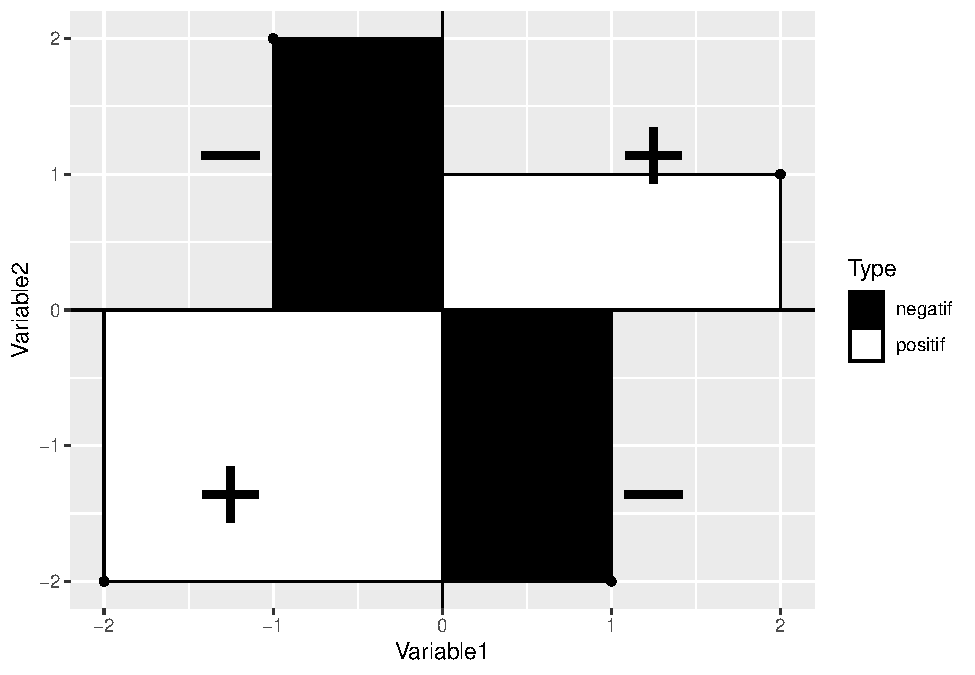
\includegraphics[width=0.75\linewidth,height=0.75\textheight]{07-Regression_files/figure-latex/unnamed-chunk-2-1} 

}

\caption{Illustration de la covariance}\label{fig:unnamed-chunk-2}
\end{figure}

\begin{figure}

{\centering 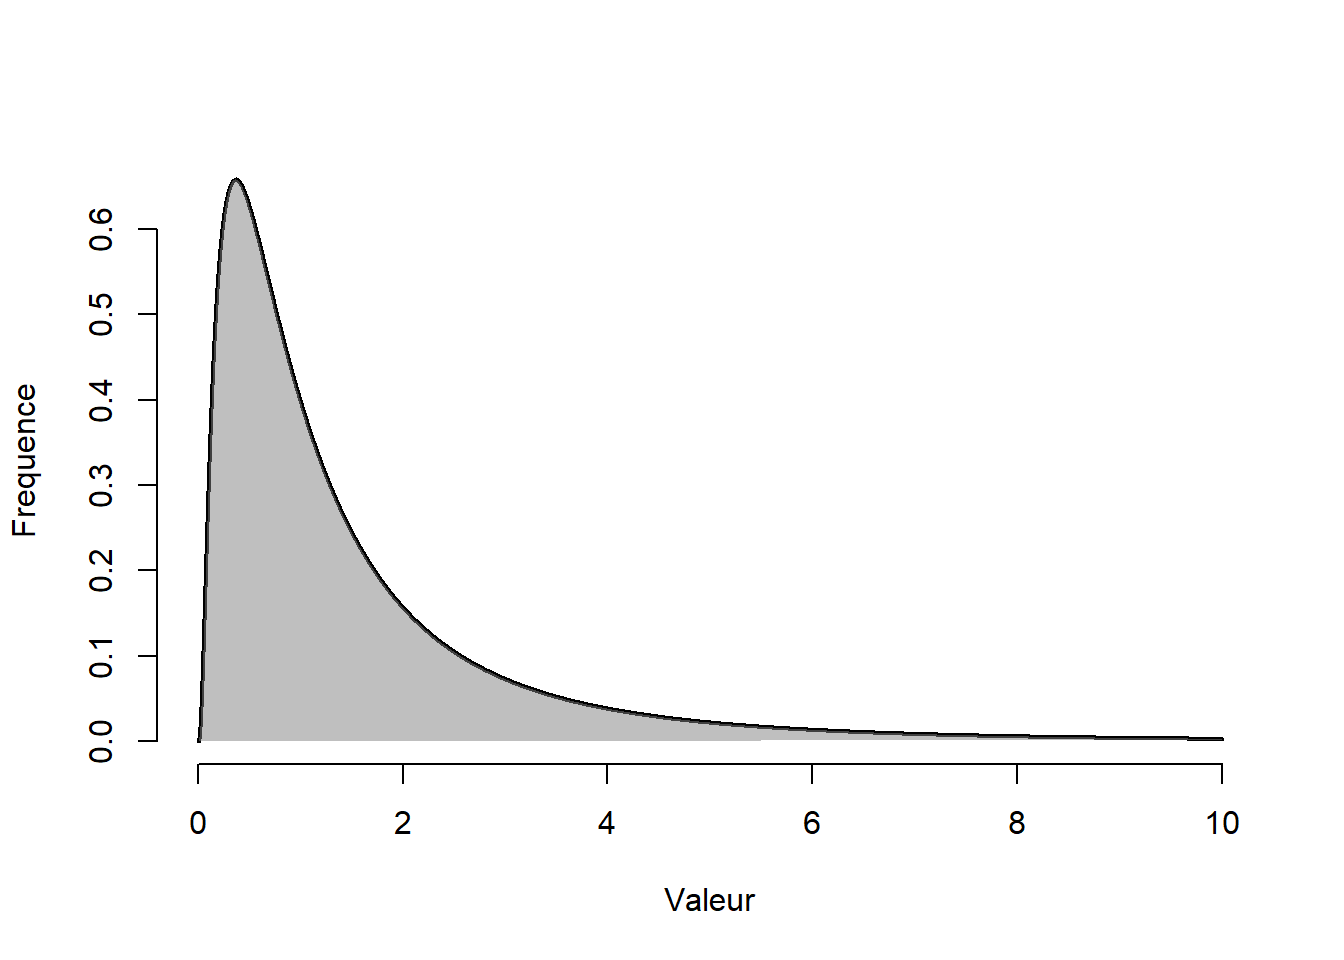
\includegraphics{07-Regression_files/figure-latex/unnamed-chunk-3-1} 

}

\caption{Illustration des produits (rectangles) pour différentes valeurs de covariance}\label{fig:unnamed-chunk-3}
\end{figure}

À partir des images suivantes, quelques propriétés de la covariance peuvent être déduites.

\begin{itemize}
\item
  Comme la quantité de surface blanche (ou de noire) dépend de la taille de la figure, la covariance est directement proportionnelle aux échelles à l'abscisse et l'ordonnée.
\item
  La covariance augmente lorsque les points s'approchent d'une ligne à pente ascendante et diminue lorsque les points s'approchent d'une ligne à pente descendante.
\item
  Comme les associations non linéaires peuvent créer des amalgames de rectangles positifs et négatifs, elles conduisent à des covariances imprévisibles et peu pertinentes.
\item
  La covariance (et la corrélation) est sensible aux valeurs aberrantes. Un point éloigné de la masse créera une aire rectangulaire bien plus grande que les autres points. À lui seul, il peut créer une quantité substantielle positive ou négative de surface blanche (ou noire) dans la figure.
\item
  Si une variable est multipliée par elle-même, il s'agit de l'aire d'un carré, ce qui équivaut au calcul d'une variance. Par extension, si le produit de deux variables se rapproche davantage d'un carré que d'un rectangle (en moyenne), alors les deux variables sont fortement liées.
\item
  Le paramètre de la corrélation de la population peut être conceptualisé comme un triangle déformé en rectangle à cause de l'erreur de mesure des axes.
\end{itemize}

\hypertarget{la-covariance-en-termes-dalguxe8bre-matricielle}{%
\subsection{La covariance en termes d'algèbre matricielle}\label{la-covariance-en-termes-dalguxe8bre-matricielle}}

Pour l'instant, seul l'aspect linéaire est présenté. L'équation de la covariance peut aussi se calculer en termes d'algèbre matricielle. En plus d'accélérer le calcul des résultats, il simplifie énormément les mathématiques sous-jante (pourvu que l'utilisateur connaisse l'algèbre matricielle).

Dans le présent contexte, une matrice est un ensemble de variables représentées sous une seule variables. Dans les équations mathématiques, une matrice est désignée par une lettre majuscule : \(x\) devient \(X\) et \(\sigma\) devient \(Sigma\). Dans une matrice, chaque colonne est une variable, chaque ligne correspond à un sujet différent mesuré sur toutes les variables. Une matrice est définie en partie par son nombre de lignes (\(n\), nombre d'unités) et son nombre de colonnes (\(p\), nombre de variables), dont voici une illustration.

\[
X = \left(\begin{array}{cccc} 
x_{1,1} & x_{1,2} & ...&x_{1,p}\\
x_{2,1} & x_{2,2} & ...&x_{2,p}\\
... & ...& ...& ... \\
x_{n,1} & x_{n,2} & ... &x_{n,p}\\
\end{array}\right)
\]

En syntaxe \textbf{R}, il ne s'agit rien de plus que de concaténer des variables (mesurant les mêmes individus) ensembles par des colonnes, comme il est fait avec des jeux de données \texttt{data.frame()} ou \texttt{cbind()}. Un jeu de données est, à peu de chose près, une matrice. Pour créer une matrice \texttt{X} à partir des variables \texttt{x}, \texttt{y}, et \texttt{z} avec \textbf{R}, par exemple, la ligne \texttt{X\ =\ cbind(x,\ y,\ z)} joindra les trois variables ensemble.

Pour réaliser le calcul de la covariance, il faut multiplier la matrice des données centrées (les variables concaténées) par elle-même puis de diviser par \(n-1\). Le symbole \(X\) représente la concaténation des variables. Par simplicité, l'équation utilise des \textbf{variables centrées}.

\begin{equation}
\Sigma = (n-1)^{-1}X^\prime X
\label{eq:covmat1}
\end{equation}

Le symbole \(\Sigma\) (sigma majuscule) représente la matrice de variance-covariance. La diagonale de cette matrice représente les variances des données et les éléments hors diagonales sont les covariances, soulignant le lien entre la variance et la covariance. Le symbole \(\prime\) (prime) correspond à l'opération de transposer une matrice, soit d'échanger les lignes par ces colonnes. Cette procédure est nécessaire pour produire la multiplication d'une matrice par elle-même. Noter que l'expression \((n-1)^{-1}=\frac{1}{n-1}\).

TODO

\begin{equation}
\begin{aligned}
S = (n-1)^{-1}
\left(\begin{array}{cccc} 
x_{1,1} & x_{2,1} & ...&x_{n,1}\\
x_{2,1} & x_{2,2} & ...&x_{n,2}\\
\end{array}\right) 
\left(\begin{array}{cc} 
x_{1,1} & x_{1,2} \\
x_{2,1} & x_{2,2}\\
... & ...  \\
x_{n,1} & x_{n,2} \\
\end{array}\right) \\
= (n-1)^{-1}
\left(\begin{array}{cc}
\sum_{i=1}^n(x_{i,1})(x_{i,1}) & \sum_{i=1}^n(x_{i,1})(x_{i,2})\\
\sum_{i=1}^n(x_{i,2})(x_{i,1}) & \sum_{i=1}^n(x_{i,2})(x_{i,2})
\end{array}\right)
\label{eq:covmat2}
\end{aligned}
\end{equation}

L'équation \eqref{eq:covmat2} illustre l'équation \eqref{eq:covmat1} qui sont toutes les deux équivalentes à \eqref{eq:cov3}. En termes de syntaxe \textbf{R}, elles peuvent être traduites comme suit.

\begin{Shaded}
\begin{Highlighting}[]
\NormalTok{covariance2 }\OtherTok{=} \ControlFlowTok{function}\NormalTok{(X)\{}
  \CommentTok{\# X est une data.frame ou matrice de n sujets par p variables}
\NormalTok{  n }\OtherTok{=} \FunctionTok{dim}\NormalTok{(X)[}\DecValTok{1}\NormalTok{]}
\NormalTok{  Xc }\OtherTok{=}\NormalTok{ X }\SpecialCharTok{{-}} \FunctionTok{colMeans}\NormalTok{(X)}
  \CommentTok{\# Algèbre matriciel pour le produit qui permet de calculer}
  \CommentTok{\# le produit d\textquotesingle{}une colonne avec les autres colonnes}
\NormalTok{  cov.X }\OtherTok{=} \FunctionTok{t}\NormalTok{(Xc) }\SpecialCharTok{\%*\%}\NormalTok{ Xc }\SpecialCharTok{/}\NormalTok{ (n }\SpecialCharTok{{-}} \DecValTok{1}\NormalTok{)}
  \FunctionTok{return}\NormalTok{(cov.X)}
\NormalTok{\}}
\end{Highlighting}
\end{Shaded}

La fonction \texttt{t()} opère la transpose (\(\prime\)) et le symbole \texttt{\%*\%} signifie le produit matriciel des variables. Si l'usuel symbole de multiplication \texttt{*} était utilisé, \textbf{R} opérerait une multiplication cellule par cellule (avec recyclage) plutôt que celle désirée ici.

L'utilisation de l'algèbre matricielle est plus simple et efficace : Elle nécessite cinq lignes de code, élimine deux boucles, prend moins de temps à calculer en plus de produire toutes les variances et les covariances.

Une matrice de covariance possède plusieurs propriétés qu'il faut connaître. Elle est toujours carrée soit \(p \times p\) pour \(p\) variables et contient \(p^2\) éléments. Parmi ces éléments, les \(p\) éléments de la diagonale sont des variances, ce pourquoi elle est parfois appelée matrice de variance-covariance. Les éléments triangulaires inférieurs hors diagonale sont un parfait reflet des éléments supérieurs, p.ex. \(\sigma_{1,2} = \sigma_{2,1}\). Il y a ainsi \(\frac{p(p-1)}{2}\) covariances uniques dans une matrice et \(p(p+1)/2\) éléments uniques (variances et covariances). En plus, de ces caractéristiques, la matrice doit être \emph{positive semi-définie}, ce qui est un terme mathématique impliquant, pour les fins de ce chapitre, que les variances ne peuvent être nulles. (C'est plus complexe que cela, mais il suffit d'accepter cette affirmation pour procéder.)

\[
\Sigma = \left( 
\begin{array}{cccc}
\sigma_{1,1} & \sigma_{1,2} & ... &  \sigma_{1,p}\\
\sigma_{2,1} & \sigma_{2,2} & ... &  \sigma_{2,p}\\
...& ...& ... &  \sigma_{3,p}\\
\sigma_{p,1} & \sigma_{p,2} & ... &  \sigma_{p,p}\\
\end{array}
\right)
\]

\hypertarget{cruxe9ation-de-donnuxe9es}{%
\subsection{Création de données}\label{cruxe9ation-de-donnuxe9es}}

Une façon simple et efficace de créer des données à ce stade est la package \texttt{MASS} dont un aperçu a été donné dans le chapitre sur les analyses de base.

\begin{Shaded}
\begin{Highlighting}[]
\CommentTok{\# Création de la matrice de covariance pour p=3}
\NormalTok{Sigma }\OtherTok{=} \FunctionTok{matrix}\NormalTok{(}\FunctionTok{c}\NormalTok{(s11, s12, s13,}
\NormalTok{                 s12, s22, s23,}
\NormalTok{                 s13, s23, s33), }\AttributeTok{nrow =} \DecValTok{3}\NormalTok{, }\AttributeTok{ncol =} \DecValTok{3}\NormalTok{)}
\CommentTok{\# Création des données }
\NormalTok{donnees }\OtherTok{=} \FunctionTok{data.frame}\NormalTok{(MASS}\SpecialCharTok{::}\FunctionTok{mvrnorm}\NormalTok{(}\AttributeTok{n =}\NormalTok{ n, }\AttributeTok{mu =} \FunctionTok{c}\NormalTok{(}\DecValTok{0}\NormalTok{,}\DecValTok{0}\NormalTok{), }\AttributeTok{Sigma =}\NormalTok{ Sigma))}
\end{Highlighting}
\end{Shaded}

La matrice de covariance pour \(p=3\) s'écrit comme suit.
\[
\Sigma = \left( 
\begin{array}{ccc}
\sigma_{1,1} & \sigma_{1,2} & \sigma_{1,3}\\
\sigma_{2,1} & \sigma_{2,2} & \sigma_{2,3}\\
\sigma_{3,1} & \sigma_{3,2} & \sigma_{2,3}
\end{array}
\right)
\]
Il convient d'écrire \(\Sigma\) (sigma majuscule) et \(\sigma\) (sigma minuscule) plutôt que \(S\), car il s'agit de la matrice de covariance de la population. Le résultat de \texttt{S\ =\ cov(donnees)} est empirique et la notation \(S\) est plus appropriée. Comme il y a \(p=3\) variables dans la syntaxe, il faudra préalablement spécifier \(3*4/2 = 6\) arguments :\(p = 3\) variances \(\sigma_{1,1},\sigma_{3,3},\sigma_{3,3}\) et \(3*2/2 =3\) covariances \(\sigma_{1,2},\sigma_{1,3},\sigma_{2,3}\).

\hypertarget{la-matrice-de-corruxe9lation}{%
\subsection{La matrice de corrélation}\label{la-matrice-de-corruxe9lation}}

Pour rappel, une matrice de corrélation est une matrice de covariance dont les variables ont été standardisées. Cela implique de transformer la matrice afin que toute la diagonale soit à l'unité, que toutes les variances soient égalent à 1. Cela permet d'avoir une interprétation \emph{standardisée} des corrélations, car celles-ci sont indépendantes des métriques originales. Les autres éléments conceptuels de la matrice de covariance s'appliquent pour la matrice de corrélation.

Pour transformer la matrice de covariance en matrice de corrélation, trois techniques sont possibles.

La première est de standardise \(X\) préalablement au calcul de la covariance. Comme il n'y a pas d'équivalent à \texttt{colMeans()} pour l'écart type, l'utilisation de \texttt{apply(X,\ MARGIN\ =\ 2,\ FUN\ =\ sd)} fera le travail. Cette ligne de syntaxe reproduit la même logique, mais pour l'écart type \texttt{sd()}. Textuellement, elle applique (\texttt{apply()}) l'écart type (\texttt{sd()}) pour chaque colonne \texttt{MARGIN\ =\ 2} à la matrice de données \texttt{X}.

\begin{Shaded}
\begin{Highlighting}[]
\NormalTok{X }\OtherTok{=}\NormalTok{ (X }\SpecialCharTok{{-}} \FunctionTok{colMeans}\NormalTok{(X)) }\SpecialCharTok{/} \FunctionTok{apply}\NormalTok{(X, }\AttributeTok{MARGIN =} \DecValTok{2}\NormalTok{, }\AttributeTok{FUN =}\NormalTok{ sd)}
\end{Highlighting}
\end{Shaded}

La deuxième méthode est de standardiser la matrice de covariance en termes d'algèbre matricielle, où \(S\) est la matrice de covariance. Il faut extraire de la matrice les variances de la diagonale (avec la fonction mathématique \(\text{diag()}\)), puis en faire la racine carrée pour obtenir des écarts types, puis en refaire une matrice carrée avec la fonction mathématique \(\text{diag()}\) qu'il faut finalement inversé pour en faire une division.

\begin{equation}
R = (\text{diag}(\sqrt{\text{diag}(S)})^{-1}) S (\text{diag}(\sqrt{\text{diag}(S)})^{-1})
\label{eq:cov2cor}
\end{equation}

En code \textbf{R}, l'équation \eqref{eq:cov2cor} se traduit ainsi.

\begin{Shaded}
\begin{Highlighting}[]
\NormalTok{R }\OtherTok{=} \FunctionTok{solve}\NormalTok{(}\FunctionTok{diag}\NormalTok{(}\FunctionTok{sqrt}\NormalTok{(}\FunctionTok{diag}\NormalTok{(S)))) }\SpecialCharTok{\%*\%}\NormalTok{ S }\SpecialCharTok{\%*\%} \FunctionTok{solve}\NormalTok{(}\FunctionTok{diag}\NormalTok{(}\FunctionTok{sqrt}\NormalTok{(}\FunctionTok{diag}\NormalTok{(S))))}
\end{Highlighting}
\end{Shaded}

Lorsqu'une matrice est passée comme argument à \texttt{diag()}, elle extrait les éléments de la diagonale pour en faire un vecteur. Si un vecteur est passé en argument, alors \texttt{diag()} retourne une matrice avec les éléments du vecteur en diagonale. La fonction \texttt{solve()} calcule l'inverse d'une matrice, comme l'utilisateur pourrait attendre de \(X^{-1}\). Il s'agit certainement de l'aspect le plus biscornu de \textbf{R}. Enfin, l'opérateur \texttt{\%*\%} est le produit matriciel.

La troisième est d'utiliser la fonction de base \texttt{cov2cor()} pour transformer la matrice de covariance en matrice de corrélation, ce qui est plus simple et plus rapide que la deuxième option, mais qui cache ce qui se réalise.

\hypertarget{la-ruxe9gression}{%
\section{La régression}\label{la-ruxe9gression}}

Pour l'instant, des rudiments de la covariance et de la corrélation ont été présentés dans le but d'introduire graduellement l'algèbre matricielle. L'objectif étant atteint, le regard portera sur la régression en tant que moyen de prédire une variable \(y\) à partir d'un ensemble de variables \(X\).

Quelle est la différence entre les analyses de covariance et corrélation comparativement à l'analyse de régression? Bien que la logique sous-jacente soit très similaire, il faut maintenant déterminer une variable \emph{différente} de l'autre, c'est-à-dire une variable dépendante. Les autres sont des variables indépendantes. Les variables indépendantes prédisent la variable dépendante un peu comme dans un modèle \emph{déterministe}, il faut décider de la cause (variables indépendantes) et l'effet (variable dépendante), ce dernier étant généré par les premiers.

Plutôt que de traiter chaque paire de variable comme c'était le cas avec l'analyse de corrélation, la régression correspond à étudier la relation entre la variable dépendante et toutes les autres, et ce, simultanément. Ainsi, les variables indépendantes sont contrôlées entre elles pour évaluer leur effet sur la variable dépendante et un modèle de prédiction plus juste est obtenu (autant que faire ce peut avec modèle statistique).

\hypertarget{le-moduxe8le-de-ruxe9gression-simple}{%
\subsection{Le modèle de régression simple}\label{le-moduxe8le-de-ruxe9gression-simple}}

L'équation pour un modèle de régression simple se résume en un cas bivarié, soit la prédiction de \(y\) par une seule variable \(x\).

\begin{equation}
y = \beta_0 + \beta_1 x + \epsilon_y
\label{eq:modlin}
\end{equation}

Dans ce modèle, \(y\) est la variable prédite, \(x\) est le seul prédicteur, \(\beta_0\) est l'ordonnée à l'origine, \(\beta_1\) est le coefficient de régression et \(\epsilon_y\), l'erreur dans la variable \(y\) indépendante (non corrélée, ni fonctionnelement liée) de \(x\).

\hypertarget{cruxe9ation-de-donnuxe9es-1}{%
\subsection{Création de données}\label{cruxe9ation-de-donnuxe9es-1}}

Une façon simple de créer des données en fonction d'un modèle linéaire plutôt qu'à partir de la matrice de corrélation (comme ce fut le case jusqu'à présent) est de reprendre l'équation \eqref{eq:modlin} et de spécifier les paramètres libre. D'abord, il faut remplacer les paramètres du modèle par des valeurs, \(beta_0\), \(beta_1\), et ensuite, créer deux variables aléatoires de taille \(n\) (la taille d'échantillon), une première pour \(x\) et une seconde pour \(\epsilon_y\). Les hypothèses sous-jacentes aux modèles linéaires assument généralement que la l'erreur (\(\epsilon\)) est distribuée normalement (avec implicitement une moyenne de 0), la fonction \texttt{rnorm()} pourra jouer le rôle. Pour \(x\), il n'y a pas de distribution à respecter, mais une distribution normale fait très bien l'affaire. Voici un exemple de code \textbf{R}.

\begin{Shaded}
\begin{Highlighting}[]
\CommentTok{\# En spécifiant une taille d\textquotesingle{}échantillon très grande,}
\CommentTok{\# l\textquotesingle{}erreur échantillonnalle est considérablement réduite.}
\CommentTok{\# Valeurs choisies par l\textquotesingle{}utilisateur}
\NormalTok{n }\OtherTok{=} \DecValTok{10000} \CommentTok{\# Taille d\textquotesingle{}échantillon}
\NormalTok{beta0 }\OtherTok{=} \DecValTok{5} \CommentTok{\# Les betas}
\NormalTok{beta1 }\OtherTok{=} \DecValTok{1}
\CommentTok{\# Deux variables aléatoires tirées de distributions normales.}
\CommentTok{\# Les moyennes sont nulles et }
\CommentTok{\# les écarts types sont spécifiés par l\textquotesingle{}utilisateur.}
\NormalTok{x }\OtherTok{=} \FunctionTok{rnorm}\NormalTok{(}\AttributeTok{n =}\NormalTok{ n, }\AttributeTok{sd =} \DecValTok{1}\NormalTok{)}
\NormalTok{e.y }\OtherTok{=} \FunctionTok{rnorm}\NormalTok{(}\AttributeTok{n =}\NormalTok{ n, }\AttributeTok{sd =} \DecValTok{3}\NormalTok{)}
\CommentTok{\# Création de la variable dépendante}
\NormalTok{y }\OtherTok{=}\NormalTok{ beta0 }\SpecialCharTok{+}\NormalTok{ beta1 }\SpecialCharTok{*}\NormalTok{ x }\SpecialCharTok{+}\NormalTok{ e.y}
\end{Highlighting}
\end{Shaded}

Si l'utilisateur souhaite ajouter une autre variable, il lui suffit d'ajouter un \(\beta\) supplémentaire et de créer une autre variable aléatoire

Cette méthode de création de données possède toutefois des limites. Principalement, elle ne spécifie pas les propriétés statistiques désirables, par exemple, la corrélation entre les variables est évacuée. Quelle est la corrélation entre \texttt{x}et \texttt{y} dans l'exemple précédent? Il est bien sûr possible de déterminer ces valeurs pour la population a posteriori. Il faut résoudre l'équation \eqref{eq:eqrho}.

\begin{equation}
\rho_{x,y} = \beta_1 \frac{\sigma_x}{\sigma_y} 
\label{eq:eqrho}
\end{equation}

Certaines valeurs sont déjà connues, car spécifiées par l'utilisateur, \(\beta_1 = 1\) et \(\sigma_x = 1\). Qu'en est-il de \(\sigma_y\)? L'utilisateur n'a pas spécifié la valeur de la variance de \(y\), il a plutôt choisi la valeur de la variance de l'erreur résiduelle, \(\sigma^2_{\epsilon_y}\). La loi de la somme des variances permettra de calculer cette valeur. Pour le lecteur intéressé, les réponses sont \(\sigma^2_y = \beta_1^2\sigma^2_x+\sigma^2_{\epsilon_y} = 10\) et donc \(\rho_{x,y} = \frac{\beta_1 \sigma_x}{\sigma_y} = 0.316\).

La limite liée à la méthode de création de données est maintenant flagrante. En plus de ne pas connaître la corrélation entre les variables, la variance de \(y\) n'est pas connue a priori. La stratégie de spécification est ainsi de choisir des valeurs et d'espérer qu'elles soient conformes aux attentes. Pire, s'il y avait plusieurs variables indépendantes, elles seraient toutes non corrélées entre elles, alors que l'utilisateur pourrait vouloir autrement, mais cette première technique ne le permet pas.

Pour l'utilisateur qui crée son jeu de données, ces caractéristiques sont souvent plus essentielles que de spécifier à l'avance la variance résiduelle. Pour résoudre cette situation, la solution est de spécifier un modèle standardisé, puis de le \emph{déstandardiser} (ajouté des moyennes et des variances a posteriori).

La philosophie de modélisation de cet ouvrage repose sur l'idée selon laquelle, un modèle doit être standardisé au départ puis \emph{déstandardisé}. Cette logique ne se prêtera pas à tous les contextes, pour certains la difficulté sera immense, pour d'autres, cela ne respectera pas les objectifs. En partant d'un modèle standardisé toutefois, la matrice de corrélation est connue à l'avance et la variance est spécifiée directement par l'utilisateur. Les tailles d'effets attendues sont également assurées. Il suffit de dériver la variance résiduelle du modèle plutôt que de la spécifier.

En assumant un modèle linéaire,

\begin{equation}
y = \beta_0 + \beta_1 x_1 + ... +\beta_k x_k + \epsilon_y
\label{eq:modling}
\end{equation}

où l'équation \eqref{eq:modling} correspond à la généralisation de l'équation \eqref{eq:modlin} pour \(k\) variables indépendantes, il est possible d'isoler \(\epsilon_y\). La variance se calcule alors comme l'équation \eqref{eq:emat}, pour le cas générale.

\begin{equation}
\sigma^2_{\epsilon_y} = \sigma^2_y - B^{\prime}RB
\label{eq:emat}
\end{equation}

où \(R\) est la matrice de corrélation et \(B\) est le vecteur contenant tous les \(\beta\) standardisés. Pour assurer un scénario standardisé \(\sigma^2_y = 1\). La seule condition sous-jacente à l'équation \eqref{eq:emat} est de s'assurer que \(\sigma^2_{\epsilon_y} > 0\), c'est-à-dire en vérifiant que \(B^{\prime}RB < \sigma^2_y\), autrement la variance est négative, ce qui est impossible. En termes de syntaxe \textbf{R}, l'équation \eqref{eq:emat} correspond à ceci.

\begin{Shaded}
\begin{Highlighting}[]
\CommentTok{\# Cacluler la variance de epsilon}
\NormalTok{var\_e }\OtherTok{=}\NormalTok{ var\_y }\SpecialCharTok{{-}} \FunctionTok{t}\NormalTok{(B) }\SpecialCharTok{\%*\%}\NormalTok{ R }\SpecialCharTok{\%*\%}\NormalTok{ B}
\end{Highlighting}
\end{Shaded}

L'avantage de cette technique est (a) de pouvoir spécifier les corrélations entre les variables indépendantes avec la matrice \(R\); (b) de déterminer à l'avance la variance de \(y\) et (c) que le vecteur \(B\) contient les \(\beta\) standardisés qui sont dans ce contexte les corrélations partielles qui relient chacune des variables indépendantes à la variable dépendante (des tailles d'effet) en contrôlant pour chacune d'elles.

L'utilisateur crée par la suite les données en spécifiant le vecteur \(B\) et en créant une variable basée sur la matrice de corrélation. Voici un exemple pour \(k=3\) variables centrées suivant une distribution normale multivariée avec la matrice de corrélation \(R\).

\[
R= \left( 
\begin{array}{ccc}
1 & .2 & .3\\
.2 & 1 & .1\\
.3 & .1 & 1
\end{array}
\right)
\]
Une fois les données de \(X\) créées, avec la fonction \texttt{MASS::mvrnorm()}, comme il a été fait précédemment, il suffit de multiplier \(X\) avec \(B\) et d'ajouter la variable aléatoire \(\epsilon_y\) avec la variance appropriée pour obtenir la variable dépendante \(y\).

\begin{Shaded}
\begin{Highlighting}[]
\FunctionTok{set.seed}\NormalTok{(}\DecValTok{42}\NormalTok{)  }\CommentTok{\# Pour reproductibilité}
\NormalTok{n }\OtherTok{=} \DecValTok{1000}      \CommentTok{\# Taille d\textquotesingle{}échantillon}
\NormalTok{k }\OtherTok{=} \DecValTok{3}         \CommentTok{\# Nombre de variables indépendantes}

\CommentTok{\# Matrice de corrélation}
\NormalTok{R }\OtherTok{=} \FunctionTok{matrix}\NormalTok{(}\FunctionTok{c}\NormalTok{(}\DecValTok{1}\NormalTok{, .}\DecValTok{2}\NormalTok{, .}\DecValTok{3}\NormalTok{,}
\NormalTok{             .}\DecValTok{2}\NormalTok{, }\DecValTok{1}\NormalTok{, .}\DecValTok{1}\NormalTok{,}
\NormalTok{             .}\DecValTok{3}\NormalTok{, .}\DecValTok{1}\NormalTok{, }\DecValTok{1}\NormalTok{), k, k)}
\CommentTok{\# Moyennes}
\NormalTok{mu }\OtherTok{=} \FunctionTok{rep}\NormalTok{(}\DecValTok{0}\NormalTok{, k)}

\CommentTok{\# Choix des betas standardisés}
\NormalTok{B }\OtherTok{=} \FunctionTok{c}\NormalTok{(}\AttributeTok{beta1 =}\NormalTok{ .}\DecValTok{2}\NormalTok{, }\AttributeTok{beta2 =} \SpecialCharTok{{-}}\NormalTok{.}\DecValTok{5}\NormalTok{, }\AttributeTok{beta3 =}\NormalTok{ .}\DecValTok{3}\NormalTok{)}

\CommentTok{\#variance de epsilon}
\NormalTok{var\_e }\OtherTok{=} \DecValTok{1} \SpecialCharTok{{-}} \FunctionTok{t}\NormalTok{(B) }\SpecialCharTok{\%*\%}\NormalTok{ R }\SpecialCharTok{\%*\%}\NormalTok{ B}

\CommentTok{\# Créations des variables aléatoires}
\NormalTok{X }\OtherTok{=}\NormalTok{ MASS}\SpecialCharTok{::}\FunctionTok{mvrnorm}\NormalTok{(}\AttributeTok{n =}\NormalTok{ n, }\AttributeTok{mu =}\NormalTok{ mu, }\AttributeTok{Sigma =}\NormalTok{ R)}
\NormalTok{e }\OtherTok{=} \FunctionTok{rnorm}\NormalTok{(}\AttributeTok{n =}\NormalTok{ n, }\AttributeTok{sd =} \FunctionTok{sqrt}\NormalTok{(var\_e))}
\CommentTok{\# Création de la variable dépendante}
\NormalTok{y }\OtherTok{=}\NormalTok{ X }\SpecialCharTok{\%*\%}\NormalTok{ B }\SpecialCharTok{+}\NormalTok{ e}

\CommentTok{\# Création du jeu de données}
\NormalTok{jd }\OtherTok{=} \FunctionTok{data.frame}\NormalTok{(}\AttributeTok{y =}\NormalTok{ y, }\AttributeTok{X =}\NormalTok{ X)}

\CommentTok{\# Quelques vérifications}
\CommentTok{\# Les données}
\FunctionTok{head}\NormalTok{(jd)}
\CommentTok{\#\textgreater{}        y    X.1    X.2     X.3}
\CommentTok{\#\textgreater{} 1  0.635 {-}0.956 {-}2.567  0.3239}
\CommentTok{\#\textgreater{} 2 {-}0.264  0.672 {-}0.172  0.5200}
\CommentTok{\#\textgreater{} 3  0.341  0.885 {-}1.369 {-}0.6387}
\CommentTok{\#\textgreater{} 4 {-}0.602  0.778 {-}1.104 {-}1.2678}
\CommentTok{\#\textgreater{} 5  0.401  0.360  0.286 {-}1.4336}
\CommentTok{\#\textgreater{} 6 {-}1.076 {-}0.210  0.621 {-}0.0399}
\CommentTok{\# La matrice de corrélation entre les variables indépendantes}
\CommentTok{\# Très près des valeurs choisies à la troisième décimale}
\FunctionTok{cor}\NormalTok{(X)}
\CommentTok{\#\textgreater{}       [,1]  [,2]  [,3]}
\CommentTok{\#\textgreater{} [1,] 1.000 0.188 0.279}
\CommentTok{\#\textgreater{} [2,] 0.188 1.000 0.136}
\CommentTok{\#\textgreater{} [3,] 0.279 0.136 1.000}
\CommentTok{\# La variance de y (encore une fois très près)}
\FunctionTok{var}\NormalTok{(y)}
\CommentTok{\#\textgreater{}      [,1]}
\CommentTok{\#\textgreater{} [1,] 1.03}
\end{Highlighting}
\end{Shaded}

Maintenant, il est possible de \emph{déstandardisé} \texttt{X} et \texttt{y} en additionnant des moyennes ou multipliant par des écarts types à chaque variable.

\hypertarget{lanalyse-de-ruxe9gression}{%
\section{L'analyse de régression}\label{lanalyse-de-ruxe9gression}}

Lorsque le jeu de données est obtenu, il est temps de procéder à l'analyse de régression. Essentiellement, l'analyse de régression produit à peu près ceci (mais en algèbre matricielle).

Pour aider la compréhension, voici une explication avec le modèle linéaire simple assumant des variables centrées. Le modèle correspond à

\[
y = \beta x
\]

où l'erreur, \(\epsilon_y\) n'est pas explicitée. Il faut isoler \(\beta\) afin de l'estimer, soit l'opération suivante,

\[
\beta = \EX(\frac{y}{x})
\]

où le symbole \(\EX\) signifie l'espérance (la moyenne). En multipliant par \(\frac{x}{x}\) de chaque côté de l'équation, cela produit l'équation suivante.

\begin{equation}
\beta = \EX(\frac{xy}{xx}) = \frac{\sigma_{xy}}{\sigma^2_x}
\label{eq:beta2}
\end{equation}

Dans l'équation \eqref{eq:beta2}, le numérateur sera rapidement reconnu comme la covariance et au dénominateur la variance de \(X\). Comment généralisé pour \(k\) variables? En algèbre matricielle et dans la mesure où les variables contenues dans \(X\) sont centrées, cela revient au même que de calculer l'équation \eqref{eq:beta}.

\begin{equation}
\hat{B} = (X^{\prime} X)^{-1} X^{\prime} y
\label{eq:beta}
\end{equation}

Comme pour l'équation \eqref{eq:beta2}, la composante \((X^{\prime} X)^{-1}\) agit en dénominateur (par l'exposant \(-1\)) et correspond à la matrice de variance-covariance des variables de \(X\) ensemble, alors que \(X^{\prime} y\) agit comme le numérateur, soit la covariance entre les variables de \(X\) avec \(y\).

Pour l'erreur type, il s'agit de calculer ceci.

\begin{equation}
\text{var}(\hat{B}) = \sigma^2 \left(X^{\prime}X\right)^{-1}
\end{equation}

La racine carrée donne l'erreur type (\emph{standard error}).

Le ratio \(\frac{B}{\text{se}_B} \sim t_{n-p-1}\), soit le quotient d'un estimateur par son erreur type, suit une distribution-\(t\) avec \(n-p-1\) degrés de liberté.

En syntaxe \textbf{R}, la régression s'écrit comme ceci.

\begin{Shaded}
\begin{Highlighting}[]
\NormalTok{regression }\OtherTok{=} \ControlFlowTok{function}\NormalTok{(y, X)\{}
  \CommentTok{\# Ajouter un intercepte}
\NormalTok{  X }\OtherTok{=} \FunctionTok{cbind}\NormalTok{(}\AttributeTok{intercept =} \DecValTok{1}\NormalTok{, X)}
\NormalTok{  B }\OtherTok{=} \FunctionTok{solve}\NormalTok{(}\FunctionTok{t}\NormalTok{(X) }\SpecialCharTok{\%*\%}\NormalTok{ X) }\SpecialCharTok{\%*\%} \FunctionTok{t}\NormalTok{(X) }\SpecialCharTok{\%*\%}\NormalTok{ y}
\NormalTok{  var.e }\OtherTok{=} \FunctionTok{var}\NormalTok{(y }\SpecialCharTok{{-}}\NormalTok{ X }\SpecialCharTok{\%*\%}\NormalTok{ B) }
\NormalTok{  se.B }\OtherTok{=} \FunctionTok{sqrt}\NormalTok{(}\FunctionTok{c}\NormalTok{(var.e) }\SpecialCharTok{*} \FunctionTok{diag}\NormalTok{(}\FunctionTok{solve}\NormalTok{(}\FunctionTok{t}\NormalTok{(X) }\SpecialCharTok{\%*\%}\NormalTok{ X)))}
\NormalTok{  n }\OtherTok{=} \FunctionTok{dim}\NormalTok{(X)[}\DecValTok{1}\NormalTok{]}
\NormalTok{  p }\OtherTok{=} \FunctionTok{dim}\NormalTok{(X)[}\DecValTok{2}\NormalTok{]}
\NormalTok{  vt }\OtherTok{=}\NormalTok{ B }\SpecialCharTok{/}\NormalTok{ se.B}
\NormalTok{  vp }\OtherTok{=}\NormalTok{ (}\DecValTok{1}\SpecialCharTok{{-}}\FunctionTok{pt}\NormalTok{(tv, }\AttributeTok{df =}\NormalTok{ n }\SpecialCharTok{{-}}\NormalTok{ p }\SpecialCharTok{{-}} \DecValTok{1}\NormalTok{)) }\SpecialCharTok{*} \DecValTok{2}
\NormalTok{  resultats }\OtherTok{=} \FunctionTok{data.frame}\NormalTok{(}\AttributeTok{Estimate =}\NormalTok{ B, }
                         \AttributeTok{Std.Error =}\NormalTok{ se.B, }
                         \AttributeTok{t.value =}\NormalTok{ vt, }
                         \AttributeTok{p.value =}\NormalTok{ vp) }
  \FunctionTok{return}\NormalTok{(resultats)}
\NormalTok{\}  }
\end{Highlighting}
\end{Shaded}

Le modèle linéaire peut aussi contenir des variables nominales dans la mesure où celle-ci sont transformées en données factices (\emph{dummy coding}). En fait, une analyse de variance n'est au fond qu'une régression dans laquelle les variables nominales sont transformées en données factices, puis utilisées en variable indépendante. Les \(\beta\) de la régression correspondent aux moyennes \(\mu\), si le participant appartient (1) à tel ou tel autre groupe ou (0) autrement. Bien que les logiciels produisent souvent des sorties statistiques différentes en fonction de l'analyse demandée, les mathématiques sous-jacentes sont les mêmes.

\hypertarget{conditions-dapplication-de-la-ruxe9gression}{%
\subsection{Conditions d'application de la régression}\label{conditions-dapplication-de-la-ruxe9gression}}

La régression possède quatre hypothèses sous-jacentes :

\begin{itemize}
\item
  La vraie relation est linéaire;
\item
  Les observations sont indépendantes.
\item
  Les résidus sont normalement distribués;
\item
  La variance résiduelle est homoscédastique.
\end{itemize}

Les deux premiers points sont davantage méthodologiques que statistiques bien que leurs conséquences soient réelles. La relation entre les variables doit être linéaire. La régression tient compte des relations en ligne droite, si la relation entre deux variables suit une courbe, elle ne pourra être adéquatement analysée. La figure \ref{fig:courbe} montre trois relations possibles entre deux variables. Bien que la relation soit très forte, peu importe la forme de la relation (les données suivent un parton très évident), seule celle au centre (relation linéaire) donnera un résultat indiquant un lien fort existant. Il existe des techniques de transformation de données lorsque ce sera \emph{théoriquement} justifié. La relation quantitative entre l'âge et la quantité de rapport sexuel est un exemple de relation non linéaire : elle débute à l'adolescence, atteint son apogée à l'âge de jeune adulte, puis décroît progressivement. La seconde hypothèse est que les unités d'observation doivent être indépendantes. Techniquement, chaque unité devrait avoir une chance égale et indépendante d'être choisie. La régression est robuste à ce genre de violation, mais il faut toujours conserver cette idée en tête lorsque le devis d'étude est conceptualisé et lors des analyses. Les élèves dans une même salle de classe ne sont techniquement pas indépendants puisqu'ils sont tous corrélés. Ils ont le même enseignant, les mêmes pairs, les locaux, etc., des variables qui peuvent toutes à leur façon avoir des effets sur les comportements des enfants. Dans ce cas, recourir à des analyses multiniveaux sera la seule possibilité pour tenir compte de cette violation et bien représenter les modèles. Un autre exemple est la corrélation entre différents temps de mesure sur une même unité (qui est corrélée avec elle-même). Dans ce cas, ce sera des analyses pour des devis temporels (les analyses multiveaux peuvent également tenir compte du temps).

Les deux autres considérations, qui sont elles d'ordre statistique, concernent les résidus (l'écart entre la prédiction et les valeurs réelles de \(y\)). Comme il a été mentionné dans la création de données pour la régression, les distributions des variables n'a pas être normales; elles peuvent suivre différentes distributions de probabilités. Par contre, l'erreur, elle, doit être normales distribuées, car il s'agit d'une hypothèse assumée de l'estimation des moindres carrés. La dernière hypothèse concerne la variance résiduelle homoscédastique, c'est-à-dire que l'écart entre les résidus et les valeurs prédites restent \emph{constantes,} peu importe le niveau sur la droite de régression. Si ce n'est pas le cas pour l'une ou l'autre, c'est qu'une variable a vraisemblablement été négligée ou qu'une des relations n'est pas linéaire avec une des variables indépendantes.

\begin{verbatim}
#> `geom_smooth()` using formula 'y ~ x'
\end{verbatim}

\begin{figure}

{\centering 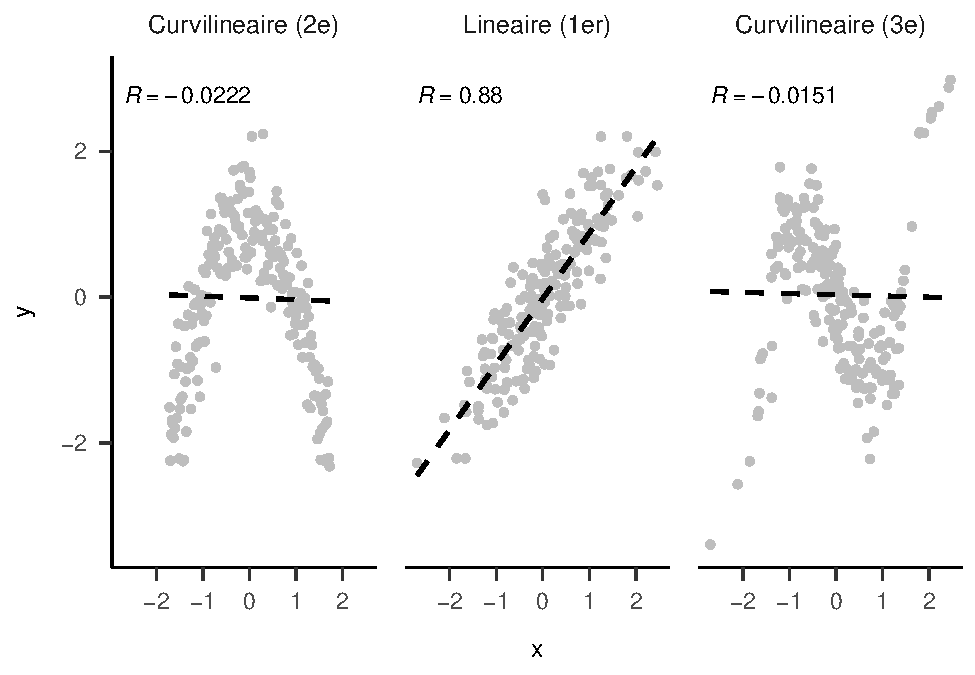
\includegraphics[width=0.8\linewidth,height=0.8\textheight]{07-Regression_files/figure-latex/courbe-1} 

}

\caption{Différentes formes de relation}\label{fig:courbe}
\end{figure}

\hypertarget{lanalyse-de-ruxe9gression-1}{%
\subsection{L'analyse de régression}\label{lanalyse-de-ruxe9gression-1}}

\textbf{R} de base offre la fonction \texttt{lm()} pour \emph{linear model} (modèle linéaire) afin de réaliser une régression. Pour réaliser l'analyse, deux éléments sont primordiaux : le jeu de données et le modèle. Le jeu de données est assez explicite. Le modèle linéaire est quant à lui déjà représenté par l'équation \eqref{eq:modling}.

Pour écrire le modèle en syntaxe \textbf{R}, il faut remplacer les \(x\) par le nom des variables dans le jeu de données, utiliser le \texttt{\textasciitilde{}} (tilde) pour délimiter les variables dépendantes à gauche des variables indépendantes à droite. Les variables indépendantes sont délimitées, comme dans l'équation \eqref{eq:modling}, par des signes d'addition \texttt{+}. Il est aussi de définir des effets d'interaction (modération) avec le signe de multiplication \texttt{*}. Les symboles \texttt{-} (soustraction) et \texttt{/} (division) ne fonctionnent pas. L'intercepte (\(\beta_0\)) est ajouté par défaut. Enfin, cette équation doit ensuite être mis entre guillemets, \texttt{formula\ =\ "y\ \textasciitilde{}\ x1\ +\ x2\ +\ x3"} pour indiquer qu'il s'agit de texte.

\begin{Shaded}
\begin{Highlighting}[]
\CommentTok{\# Créer un jeu de données à partir des variables de la syntaxe précédente}
\NormalTok{res.lm }\OtherTok{=} \FunctionTok{lm}\NormalTok{(}\AttributeTok{formula =}\NormalTok{ y }\SpecialCharTok{\textasciitilde{}}\NormalTok{ X}\FloatTok{.1} \SpecialCharTok{+}\NormalTok{ X}\FloatTok{.2} \SpecialCharTok{+}\NormalTok{ X}\FloatTok{.3}\NormalTok{, }\AttributeTok{data =}\NormalTok{ jd)}
\CommentTok{\# Les résultats}
\NormalTok{res.lm}
\CommentTok{\#\textgreater{} }
\CommentTok{\#\textgreater{} Call:}
\CommentTok{\#\textgreater{} lm(formula = y \textasciitilde{} X.1 + X.2 + X.3, data = jd)}
\CommentTok{\#\textgreater{} }
\CommentTok{\#\textgreater{} Coefficients:}
\CommentTok{\#\textgreater{} (Intercept)          X.1          X.2          X.3  }
\CommentTok{\#\textgreater{}     {-}0.0171       0.2139      {-}0.5520       0.3095}
\CommentTok{\# Sommaire des résultats}
\FunctionTok{summary}\NormalTok{(res.lm)}
\CommentTok{\#\textgreater{} }
\CommentTok{\#\textgreater{} Call:}
\CommentTok{\#\textgreater{} lm(formula = y \textasciitilde{} X.1 + X.2 + X.3, data = jd)}
\CommentTok{\#\textgreater{} }
\CommentTok{\#\textgreater{} Residuals:}
\CommentTok{\#\textgreater{}     Min      1Q  Median      3Q     Max }
\CommentTok{\#\textgreater{} {-}2.5227 {-}0.5546 {-}0.0119  0.5513  2.5762 }
\CommentTok{\#\textgreater{} }
\CommentTok{\#\textgreater{} Coefficients:}
\CommentTok{\#\textgreater{}             Estimate Std. Error t value Pr(\textgreater{}|t|)    }
\CommentTok{\#\textgreater{} (Intercept)  {-}0.0171     0.0253   {-}0.68      0.5    }
\CommentTok{\#\textgreater{} X.1           0.2139     0.0266    8.03  2.7e{-}15 ***}
\CommentTok{\#\textgreater{} X.2          {-}0.5520     0.0258  {-}21.42  \textless{} 2e{-}16 ***}
\CommentTok{\#\textgreater{} X.3           0.3095     0.0263   11.76  \textless{} 2e{-}16 ***}
\CommentTok{\#\textgreater{} {-}{-}{-}}
\CommentTok{\#\textgreater{} Signif. codes:  }
\CommentTok{\#\textgreater{} 0 \textquotesingle{}***\textquotesingle{} 0.001 \textquotesingle{}**\textquotesingle{} 0.01 \textquotesingle{}*\textquotesingle{} 0.05 \textquotesingle{}.\textquotesingle{} 0.1 \textquotesingle{} \textquotesingle{} 1}
\CommentTok{\#\textgreater{} }
\CommentTok{\#\textgreater{} Residual standard error: 0.8 on 996 degrees of freedom}
\CommentTok{\#\textgreater{} Multiple R{-}squared:  0.383,  Adjusted R{-}squared:  0.381 }
\CommentTok{\#\textgreater{} F{-}statistic:  206 on 3 and 996 DF,  p{-}value: \textless{}2e{-}16}
\end{Highlighting}
\end{Shaded}

Pour ajouter une variable il suffit de \texttt{VD\ \textasciitilde{}\ VI1\ +\ VI2}; pour ajouter un effet d'interaction, il est possible de faire \texttt{VD\ \textasciitilde{}\ VI1\ *\ VI2}. Pour ajouter une variable nominale (catégorielle), il suffit d'ajouter la variable comme n'importe quelles autres \texttt{x}, mais en s'assurant bien qu'elle soit désignée comme un facteur dans le jeu de données. Si ce n'était pas le cas, la fonction \texttt{as.factor()} devrait corriger la situation.

La fonction \texttt{lm()} en elle-même n'imprime que peut de résultats. Pour obtenir l'information complète, il faut requérir le sommaire avec la fonction \texttt{summary()}. Le sommaire des résultats contient toute l'information qu'un expérimentateur peut désirer. Il y a les coefficients de régression \texttt{Estimate}, leur erreur standard \texttt{Std.\ Error}, leur valeur-\(t\) \texttt{t\ value} et leur valeur-\(p\) \texttt{Pr(\textgreater{}\textbar{}t\textbar{})}. Tout cela peut être extrait avec \texttt{summary(res.lm)\$...} en remplaçant \texttt{...} par les éléments désirés. Au-dessous de la sortie imprimée, il y a également le coefficient de détermination (\(R^2\), \texttt{R-squared}), les degrés de liberté et la valeur-\(p\) associé au modèle.

Un manuscrit pourrait rapport les résultats ainsi. Le modèle tester obtient un coefficient de détermination de \(R^2(996) = 0.383, p < .001\). Les trois prédicteurs sont liés significativement à la variable dépendante, respectivement \(X_1: \beta_1 = 0.214, p = < .001\), \(X_2: \beta_2 = 0.214, p = < .001\), \(X_3: \beta_3 = 0.31, p = < .001\). Évidemment, comme l'exemple est artificiel, il y a peu de chose à dire sans devoir fabriquer de toutes pièces des interprétations alambiquées bien que cela fût fort bénéfique pour la carrière de certains psychanalystes.

Pour vérifier la qualité des résultats, il faut vérifier la distribution des résidus. Pour ce faire, il faut extraire les résidus et les valeurs prédites. Pour la création de graphiques, il est plus simple d'ajouter ces scores au jeu de données. Les fonctions \texttt{resid()} et \texttt{predict()} permettront d'extraire les résidus et les prédictions en y insérant comme argument le sommaire de la fonction \texttt{lm()} obtenu avec les données.

\begin{Shaded}
\begin{Highlighting}[]
\CommentTok{\# Ajouter les résidus et scores prédits à la base de données}
\CommentTok{\# avec la fonction \textasciigrave{}resid()\textasciigrave{}}
\NormalTok{jd}\SpecialCharTok{$}\NormalTok{residu }\OtherTok{=} \FunctionTok{resid}\NormalTok{(res.lm)}
\NormalTok{jd}\SpecialCharTok{$}\NormalTok{predit }\OtherTok{=} \FunctionTok{predict}\NormalTok{(res.lm)}
\end{Highlighting}
\end{Shaded}

Une fois, c'est valeur extraite, le package \texttt{ggplot2} permet de réaliser rapidement des graphiques, comme le diagramme de dispersion à la figure \ref{fig:respred} ou l'histogramme des résidus à la figure \ref{fig:reshist}. Dans les meilleures situations, les résidus seront distribués normalement dans l'histogramme et aucune tendance ne devrait être discernable dans le diagramme de dispersion. Si ce n'était pas le cas, il pourrait y avoir un problème à élucider, par exemple, une relation non linéaire imprévue. Les figures \ref{fig:respred} et \ref{fig:reshist} ne signale aucun problème, ce qui est attendu considérant la création des données employées.

\begin{Shaded}
\begin{Highlighting}[]
\CommentTok{\# Diagramme de dispersion prédits par résidus}
\NormalTok{jd }\SpecialCharTok{\%\textgreater{}\%} 
  \FunctionTok{ggplot}\NormalTok{(}\AttributeTok{mapping =} \FunctionTok{aes}\NormalTok{(}\AttributeTok{x =}\NormalTok{ predit, }\AttributeTok{y =}\NormalTok{ residu)) }\SpecialCharTok{+} 
  \FunctionTok{geom\_point}\NormalTok{() }
\end{Highlighting}
\end{Shaded}

\begin{figure}

{\centering 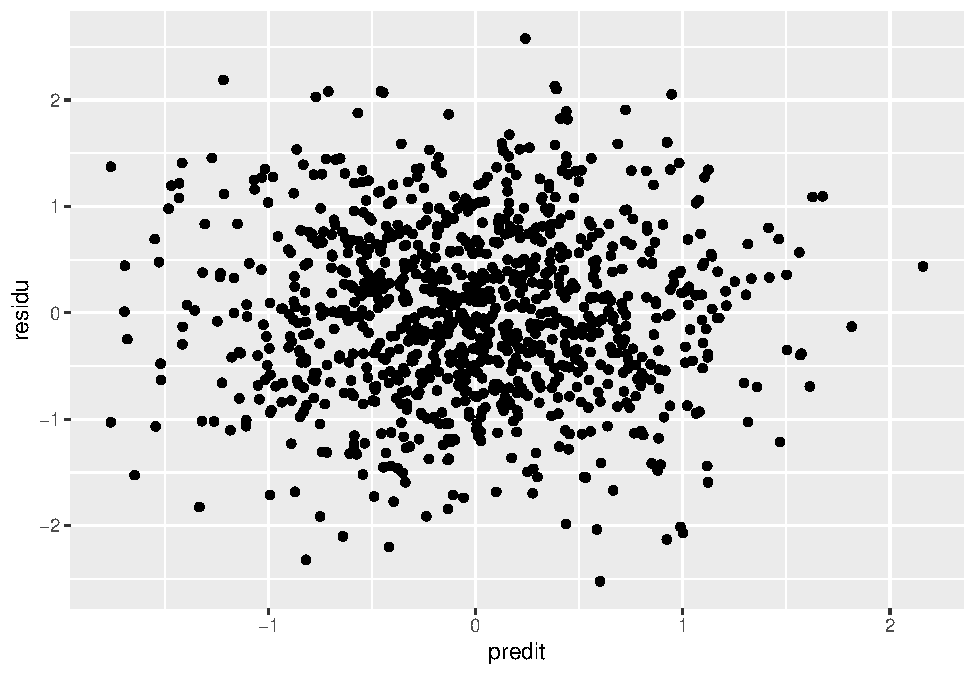
\includegraphics[width=0.75\linewidth,height=0.75\textheight]{07-Regression_files/figure-latex/respred-1} 

}

\caption{Relation entre prédicitons et résidus}\label{fig:respred}
\end{figure}

\begin{Shaded}
\begin{Highlighting}[]
\CommentTok{\# Histogramme des résidus}
\NormalTok{jd }\SpecialCharTok{\%\textgreater{}\%} 
  \FunctionTok{ggplot}\NormalTok{(}\AttributeTok{mapping =} \FunctionTok{aes}\NormalTok{(}\AttributeTok{x =}\NormalTok{ residu)) }\SpecialCharTok{+} 
  \FunctionTok{geom\_histogram}\NormalTok{()}
\end{Highlighting}
\end{Shaded}

\begin{figure}

{\centering 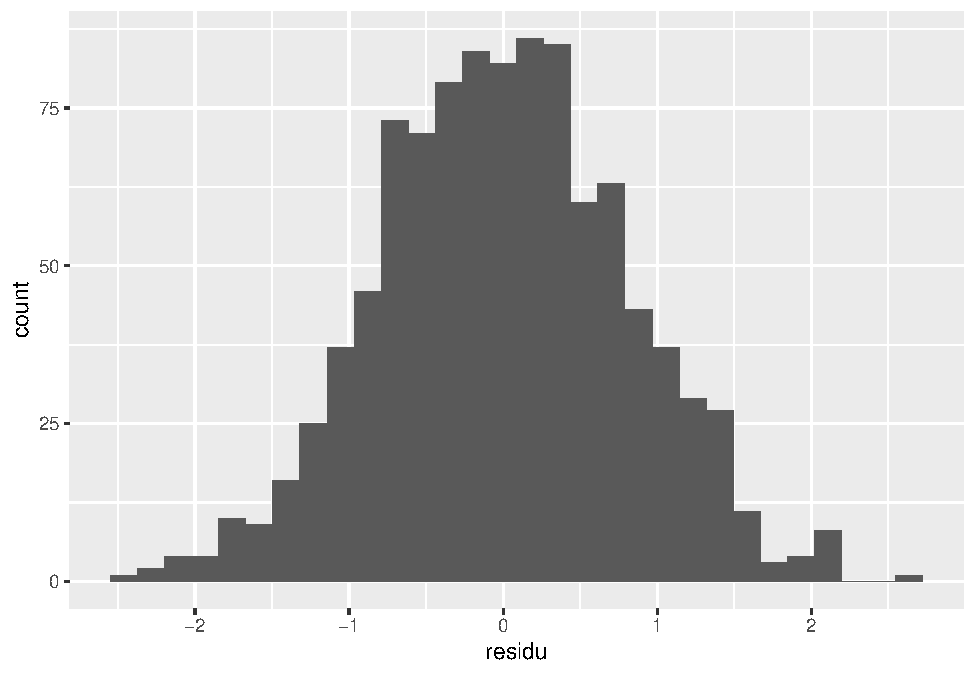
\includegraphics[width=0.75\linewidth,height=0.75\textheight]{07-Regression_files/figure-latex/reshist-1} 

}

\caption{Histogramme des résidus}\label{fig:reshist}
\end{figure}

\hypertarget{solutions}{%
\chapter*{Solutions}\label{solutions}}
\addcontentsline{toc}{chapter}{Solutions}

\hypertarget{partie-1}{%
\section*{Partie 1}\label{partie-1}}
\addcontentsline{toc}{section}{Partie 1}

\begin{quote}
\begin{enumerate}
\def\labelenumi{\arabic{enumi}.}
\tightlist
\item
  Quel est le résultat de \texttt{mean\ \textless{}-\ c(1,\ 2,\ 3)}? Pourquoi?
\end{enumerate}
\end{quote}

Le résultat est \(1, 2, 3\). Le fait d'assigner une valeur à une fonction (ou variable) écrase cette dernière.

\begin{Shaded}
\begin{Highlighting}[]
\NormalTok{mean }\OtherTok{\textless{}{-}} \FunctionTok{c}\NormalTok{(}\DecValTok{1}\NormalTok{, }\DecValTok{2}\NormalTok{, }\DecValTok{3}\NormalTok{)}
\NormalTok{mean}
\CommentTok{\#\textgreater{} [1] 1 2 3}
\end{Highlighting}
\end{Shaded}

\begin{quote}
\begin{enumerate}
\def\labelenumi{\arabic{enumi}.}
\setcounter{enumi}{1}
\tightlist
\item
  Rédiger une fonction calculant l'hypoténuse d'un triangle rectangle. Rappel, le théorème de Pythagore est \(c^2=a^2+b^2\).
\end{enumerate}
\end{quote}

En prenant \texttt{a} et \texttt{b} comme arguments.

\begin{Shaded}
\begin{Highlighting}[]
\NormalTok{hypothenus }\OtherTok{\textless{}{-}} \ControlFlowTok{function}\NormalTok{(a, b)\{}
  \FunctionTok{sqrt}\NormalTok{(a}\SpecialCharTok{\^{}}\DecValTok{2} \SpecialCharTok{+}\NormalTok{ b}\SpecialCharTok{\^{}}\DecValTok{2}\NormalTok{)}
\NormalTok{\}}
\FunctionTok{hypothenus}\NormalTok{(}\DecValTok{3}\NormalTok{, }\DecValTok{4}\NormalTok{)}
\CommentTok{\#\textgreater{} [1] 5}
\end{Highlighting}
\end{Shaded}

\begin{quote}
\begin{enumerate}
\def\labelenumi{\arabic{enumi}.}
\setcounter{enumi}{2}
\tightlist
\item
  Rédiger une fonction calculant un score-\(z\) pour une variable. Rappel, un score-\(z\), correspond à \(z=\frac{x-\mu}{\sigma}\).
\end{enumerate}
\end{quote}

Deux possibilités ici. Soit \texttt{x} est un vecteur contenant plusieurs nombres ou il est un nombre et il faut ajouter la moyenne (\(\mu\)) et l'écart type (\(\sigma\)).

\begin{Shaded}
\begin{Highlighting}[]
\CommentTok{\# Premier cas}
\NormalTok{score.z }\OtherTok{\textless{}{-}} \ControlFlowTok{function}\NormalTok{(x) \{}
\NormalTok{  (x}\SpecialCharTok{{-}}\FunctionTok{mean}\NormalTok{(x))}\SpecialCharTok{/}\FunctionTok{sd}\NormalTok{(x)}
\NormalTok{\} }

\CommentTok{\# Deuxième cas}
\NormalTok{score.z }\OtherTok{\textless{}{-}} \ControlFlowTok{function}\NormalTok{(x, mu, sigma) \{}
\NormalTok{  (x}\SpecialCharTok{{-}}\NormalTok{mu)}\SpecialCharTok{/}\NormalTok{sigma}
\NormalTok{\} }

\FunctionTok{score.z}\NormalTok{(}\DecValTok{130}\NormalTok{, }\AttributeTok{mu =} \DecValTok{100}\NormalTok{, }\AttributeTok{sigma =} \DecValTok{15}\NormalTok{)}
\CommentTok{\#\textgreater{} [1] 2}
\end{Highlighting}
\end{Shaded}

Le premier cas est l'équivalent de la fonction \texttt{scale()} qui rempliera la même tâche.

\begin{quote}
\begin{enumerate}
\def\labelenumi{\arabic{enumi}.}
\setcounter{enumi}{3}
\tightlist
\item
  Rédiger une fonction calculant la médiane d'une variable (ne recopier pas celle de ce livre).
\end{enumerate}
\end{quote}

Voici une autre fonction calculant une médiane d'un vecteur.

\begin{Shaded}
\begin{Highlighting}[]
\NormalTok{mediane }\OtherTok{\textless{}{-}} \ControlFlowTok{function}\NormalTok{(x)\{}
\NormalTok{  x }\OtherTok{\textless{}{-}} \FunctionTok{sort}\NormalTok{(x)}
\NormalTok{  longueur }\OtherTok{\textless{}{-}} \FunctionTok{length}\NormalTok{(x)}
  \ControlFlowTok{if}\NormalTok{ (longueur}\SpecialCharTok{\%\%}\DecValTok{2}\NormalTok{) \{}
    \CommentTok{\# Si impair}
    \CommentTok{\# Prendre la valeur centrale}
\NormalTok{    x[(longueur }\SpecialCharTok{+} \DecValTok{1}\NormalTok{)}\SpecialCharTok{/}\DecValTok{2}\NormalTok{]}
\NormalTok{  \} }\ControlFlowTok{else}\NormalTok{ \{}
    \CommentTok{\# Si pair}
    \CommentTok{\# Faire la moyenne des deux éléments du centre}
    \FunctionTok{mean}\NormalTok{(x[}\FunctionTok{rep}\NormalTok{(longueur}\SpecialCharTok{/}\DecValTok{2}\NormalTok{, }\DecValTok{2}\NormalTok{) }\SpecialCharTok{+} \DecValTok{0}\SpecialCharTok{:}\DecValTok{1}\NormalTok{])}
\NormalTok{  \}}
\NormalTok{\}}
\end{Highlighting}
\end{Shaded}

Encore une fois (il n'y a pas vraiment de façon de l'éviter), \texttt{\%\%2} permet de tester si pair (\texttt{FALSE}, car \texttt{0} si pair) ou impair (\texttt{TRUE}, car \texttt{1} si impair), puis de prendre la valeur à la position correspondante. Il y a plusieurs façons de tirer les éléments du vecteur.

\begin{quote}
\begin{enumerate}
\def\labelenumi{\arabic{enumi}.}
\setcounter{enumi}{4}
\tightlist
\item
  Rédiger une fonction pour générer une séquence de Fibonacci (chaque nombre est la somme des deux précédents) jusqu'à une certaine valeur, soit \(1,1,2,3,5,8,...\).
\end{enumerate}
\end{quote}

Plusieurs solutions possibles dont en voici deux.

\begin{Shaded}
\begin{Highlighting}[]
\NormalTok{fibonnaci1 }\OtherTok{\textless{}{-}}  \ControlFlowTok{function}\NormalTok{(n)\{}
  \CommentTok{\# n est le nombre d\textquotesingle{}éléments de la série demandée.}
  \CommentTok{\# Création d\textquotesingle{}un vecteur de taille n ne contenant que des 1.}
\NormalTok{  serie }\OtherTok{\textless{}{-}} \FunctionTok{rep}\NormalTok{(}\DecValTok{1}\NormalTok{, n)}
  \CommentTok{\# Le premier test logique rapporte la (n = 1) ou }
  \CommentTok{\# les deux (n = 2) premières valeurs.}
  \ControlFlowTok{if}\NormalTok{(n }\SpecialCharTok{\textless{}=} \DecValTok{2}\NormalTok{)\{}
\NormalTok{    serie }\OtherTok{\textless{}{-}}\NormalTok{  serie[}\DecValTok{1}\SpecialCharTok{:}\NormalTok{n]}
    \CommentTok{\# Le deuxième réalise les calculs pour les autres options.  }
\NormalTok{  \}}\ControlFlowTok{else}\NormalTok{\{}
    \ControlFlowTok{for}\NormalTok{(i }\ControlFlowTok{in} \DecValTok{3}\SpecialCharTok{:}\NormalTok{n)\{}
\NormalTok{      serie[i] }\OtherTok{\textless{}{-}}\NormalTok{  serie[i}\DecValTok{{-}1}\NormalTok{] }\SpecialCharTok{+}\NormalTok{ serie[i}\DecValTok{{-}2}\NormalTok{]  }
\NormalTok{    \}}
\NormalTok{  \}}
\NormalTok{  serie}
\NormalTok{\}}
\end{Highlighting}
\end{Shaded}

En voici une autre en utilisant la récursion (une fonction qui s'appelle elle-même).

\begin{Shaded}
\begin{Highlighting}[]
\NormalTok{fibonnaci2 }\OtherTok{\textless{}{-}} \ControlFlowTok{function}\NormalTok{(n)\{}
  \ControlFlowTok{if}\NormalTok{(n }\SpecialCharTok{\textless{}=} \DecValTok{2}\NormalTok{)\{}
    \CommentTok{\# Si la n est plus petit que 2, alors retourne 1}
    \DecValTok{1}
\NormalTok{  \} }\ControlFlowTok{else}\NormalTok{ \{}
    \CommentTok{\# Autrement, retourne, les deux valeurs de Fibonncaci précédentes.}
    \FunctionTok{fibonnaci2}\NormalTok{(n}\DecValTok{{-}1}\NormalTok{) }\SpecialCharTok{+} \FunctionTok{fibonnaci2}\NormalTok{ (n}\DecValTok{{-}2}\NormalTok{)}
\NormalTok{  \}}
\NormalTok{\}}
\end{Highlighting}
\end{Shaded}

Les voici comparées.

\begin{Shaded}
\begin{Highlighting}[]
\NormalTok{n }\OtherTok{\textless{}{-}} \DecValTok{8}
\FunctionTok{fibonnaci1}\NormalTok{(n)}
\CommentTok{\#\textgreater{} [1]  1  1  2  3  5  8 13 21}
\FunctionTok{fibonnaci2}\NormalTok{(n)}
\CommentTok{\#\textgreater{} [1] 21}
\end{Highlighting}
\end{Shaded}

\begin{quote}
\begin{enumerate}
\def\labelenumi{\arabic{enumi}.}
\setcounter{enumi}{5}
\tightlist
\item
  Rédiger une fonction qui pivote une liste de \(k\) éléments par \(n\). Par exemple, une liste de six (\(k=6\) comme \([1,2,3,4,5,6]\)) pivoté de deux (\(n=2\)) devient (\([3,4,5,6,1,2]\)).
\end{enumerate}
\end{quote}

Plusieurs solutions possibles dont en voici une.

\begin{Shaded}
\begin{Highlighting}[]
\NormalTok{pivot }\OtherTok{\textless{}{-}} \ControlFlowTok{function}\NormalTok{(k, n)\{}
\NormalTok{  pivoter }\OtherTok{\textless{}{-}} \FunctionTok{c}\NormalTok{((n}\SpecialCharTok{+}\DecValTok{1}\NormalTok{)}\SpecialCharTok{:}\NormalTok{k, }\DecValTok{1}\SpecialCharTok{:}\NormalTok{n)}
\NormalTok{  pivoter}
\NormalTok{\}}
\CommentTok{\# Original}
\NormalTok{k }\OtherTok{\textless{}{-}} \DecValTok{6}
\DecValTok{1}\SpecialCharTok{:}\NormalTok{k}
\CommentTok{\#\textgreater{} [1] 1 2 3 4 5 6}

\CommentTok{\# Pivoté}
\FunctionTok{pivot}\NormalTok{(}\AttributeTok{k =}\NormalTok{ k, }\AttributeTok{n =} \DecValTok{2}\NormalTok{)}
\CommentTok{\#\textgreater{} [1] 3 4 5 6 1 2}
\end{Highlighting}
\end{Shaded}

\hypertarget{partie-2}{%
\section*{Partie 2}\label{partie-2}}
\addcontentsline{toc}{section}{Partie 2}

\printbibliography

\end{document}
